\documentclass[twoside,openright,12pt]{book}
\usepackage[a4paper,top=25mm,bottom=25mm,left=40mm,right=25mm,bindingoffset=0mm,headheight=14.5pt,headsep=12pt]{geometry}
\usepackage[utf8]{inputenc}
\usepackage{graphicx}
\graphicspath{{images/}}
\usepackage{subfig}
% \captionsetup[subfigure]{subrefformat=simple,labelformat=simple,listofformat=subsimple}
% \renewcommand\thesubfigure{(\alph{subfigure})}
\usepackage{amsthm,amssymb,mathptmx}
\usepackage{fancyhdr}
\pagestyle{fancy}
\fancyhf{}
\renewcommand{\headrulewidth}{1pt} % optional
\renewcommand{\footrulewidth}{1pt} % optional
\fancyhead[LE,RO]{\nouppercase{\footnotesize \leftmark}}
\fancyfoot[C]{\nouppercase{\thepage}}
\fancyfoot[LE,RO]{\scriptsize{Harikrishnan Magarabooshanam}}
\newcounter{savepage}
\usepackage[auto]{chappg}
\usepackage{setspace}
\usepackage{epstopdf} %%package to overcome problem with eps in pdf files
% \usepackage{babel}
\usepackage[nottoc,numbib]{tocbibind}
\usepackage[
	backend=biber,
	firstinits=false,
	maxcitenames=2,
	maxbibnames=99,
	citestyle=authoryear-comp,
	giveninits=true,
	uniquename=false,
	uniquelist=false,
	url=false,
	natbib=true,
	style=authoryear,
	dashed=false,
	sorting=nyt]{biblatex}
\DeclareNameAlias{default}{family-given}
% \DeclareFieldFormat{labelnumberwidth}{}
% \setlength{\biblabelsep}{0pt}
\bibliography{library}
\usepackage{hyperref}
\hypersetup{
	colorlinks   = true, %Colours links instead of ugly boxes
	urlcolor     = [RGB]{0,51,153}, %Colour for external hyperlinks
	linkcolor    = [RGB]{0,51,153}, %Colour of internal links
	citecolor   = red %Colour of citations
}
\usepackage{emptypage}
\usepackage{gensymb}
\usepackage{booktabs}
\usepackage{amsmath}
\usepackage{multirow}
\newcommand{\minitab}[2][l]{\begin{tabular}{#1}#2\end{tabular}}
\usepackage{array}
\usepackage[noabbrev]{cleveref}
\usepackage{listings}
\usepackage{enumitem}
\usepackage{lscape}
\usepackage[flushleft]{threeparttable}
\usepackage{tabularx}
\usepackage{caption}
\usepackage{fontenc}
\usepackage{tikz}
\usetikzlibrary{calc}
% \usepackage{subcaption}
\usepackage[counterclockwise, figuresright]{rotating}
\setcounter{tocdepth}{3}
\setcounter{secnumdepth}{3}
%\addbibresource{library.bib}

\makeatletter
\def\cleardoublepage{\clearpage%
	\if@twoside
	\ifodd\c@page\else
	\vspace*{\fill}
	\hfill
	\begin{center}
		[This page is intentionally left blank]
	\end{center}
	\vspace{\fill}
	\thispagestyle{empty}
	\newpage
	\if@twocolumn\hbox{}\newpage\fi
	\fi
	\fi
}
\makeatother
\begin{document}

\pagenumbering{roman}

\begin{titlepage}
    \begin{tikzpicture}[remember picture, overlay]
      \draw[line width = 1 pt] ($(current page.north west) + (40mm,-25mm)$) rectangle ($(current page.south east) + (-25mm,25mm)$);
      \draw[line width = 1 pt] ($(current page.north west) + (38mm,-23mm)$) rectangle ($(current page.south east) + (-23mm,23mm)$);
      \end{tikzpicture}
    \begin{center}
        \vspace*{0.5cm}
        \Huge
        \textbf{Fire Performance of Complex Light Gauge Steel Framed Wall Systems}
        
        \vspace{1cm}
        \Large
        By
        
        \vspace{1cm}
        \LARGE
        \textbf{Harikrishnan Magarabooshanam}
        \vspace{1.5cm}
        
        
\includegraphics[width=0.3\textwidth]{QUTlogo.pdf}
        
        \vspace{1cm}
        \large
        \centering \textit{A thesis submitted to the\\ School of Civil and Environmental Engineering,\\ Queensland University of Technology \\in fulfilment of the requirements for the degree of}\\
        \vspace{1cm}
        \LARGE
       \textbf{ Doctor of Philosophy}
        \vspace{1cm}
        
      \linespread{1.2}
      \small    
        School of Civil and Environmental Engineering\\   
        Science and Engineering Faculty\\     
        Queensland University of Technology\\        
        Australia\\
        2020 
    \end{center}
\end{titlepage}

\chapter*{Keywords}
\addcontentsline{toc}{chapter}{Keywords}
{\setstretch{1.5}

Complex Light gauge steel-framed (LSF) walls, Cold-formed steel, Double stud, Staggered stud, Shaftliner, Time-temperature curve, Buckling, Load bearing, Non-load bearing Fire Dynamics Simulator (FDS), Effective cavity depth, Stud depth, Convection, Load ratio, Fire Resistance Level (FRL).  

}

\chapter*{Abstract}{\setstretch{1.5}}
\addcontentsline{toc}{chapter}{Abstract}
{\setstretch{1.5}

Cold-formed steel in the Australian construction industry is experiencing a phenomenal growth. In the residential sector light gauge steel framed (LSF) walls with single stud arrangement are commonly used as load bearing and non-load bearing walls. But in situations where higher acoustic insulation levels and load bearing capacities are required such as theatres, hospitals and town houses, complex LSF walls including double stud, shaftliner and staggered stud LSF walls are used. However, fire performance of these complex LSF walls has not been investigated adequately unlike in the case of single stud LSF walls. Fire resistance of LSF wall systems is important in the emerging mid-rise cold-formed steel construction. Many studies have been conducted in recent times to improve the acoustic, thermal (energy) and fire performance of non-load bearing LSF walls. Increasing the wall cavity depth provides superior acoustic and thermal performance characteristics of LSF walls. There is insufficient research data on the fire performance of these wall systems. The problems in determining the fire performance of these LSF walls have been identified and the investigations conducted in addressing the same are summarised below.   

Firstly, this research investigated the fire performance of complex LSF walls under standard fire conditions using full scale test panels (3 m \(\times\) 3 m) made of lipped channel studs. Ten full-scale fire tests were conducted to investigate the fire performance of load bearing and non load bearing double stud, shaftliner and staggered stud walls. Ambient capacity tests on the double and staggerd stud walls were also conducted to determine the ambient temperature axial load carrying capacities of these walls. Direct Strength Method based design capacity equations were also used to determine the ambient temperature axial compression capacities of these complex LSF wall systems and their suitability was also investigated. The fire test results of double stud, shaftliner and staggered stud LSF walls were then compared with those of single stud LSF walls with varying stud depth. The fire test results revealed the presence of a unique heat transfer mechanism, resulting in an enhanced fire performance for these complex LSF walls. The discontinuous stud arrangement within the cavity of double stud LSF walls was identified as the main contributor for the delayed heat transfer mechanism. Fire test results show that the temperatures across the wall depth decrease with increasing cavity depth. LSF walls with two layers of plasterboard lining and wider cavity resulted in increased fire resistance. This research also highlights the detrimental effects of staggered stud LSF wall arrangement causing structural failure of thin-walled steel studs. 

Cavity insulation is an integral part of the LSF wall system. However, the fire performance of the cavity insulated LSF walls are often misunderstood. Past research studies have investigated the fire performance of cavity insulated LSF walls. But, the research studies were again limited to LSF walls with single row of studs. Often, cavity insulated double and staggered stud LSF walls are used as partition walls in apartments under load bearing conditions and understanding their structural behaviour when exposed to fire becomes utmost necessity. This research study has also focused on investigating the fire performance of cavity insulated double stud LSF walls exposed to fire under load bearing conditions through full-scale fire tests. Attempts were also made to alter the position of the insulation within the cavity and investigate the effects through full-scale fire tests. This included positioning the insulation on the ambient side of the test wall and also by arranging it in a staggered pattern.

Since conducting full-scale fire tests are expensive and time consuming there arises a need to develop a robust numerical model to determine the thermal and structural performance of these complex LSF walls. Therefore attempts were made to develop numerical models in SAFIR, ABAQUS and FDS to determine the thermal performance of these complex LSF walls. The conventional thermal models developed through finite element (FE) method in ABAQUS was suitable for predicting the thermal behaviour of conventional single stud LSF walls. However, these models had many limitations such as neglecting the effects of convection within the cavity and longer computational time. Likewise the SAFIR thermal model over predicted the time-temperature curves. Also, the effects of radiation were assumed to be predominant mode of heat transfer within the cavity. Despite these limitations these models were used to validate single stud LSF wall fire tests as the effect of convection was less in these walls. However, the presence of discontinuous stud arrangements within the cavity complicates the situation making the current FE thermal models to become ineffective in predicting the thermal performance of the complex LSF walls. It was found that the complex heat transfer mechanism in these LSF walls could be better simulated with FDS. Validations of the thermal models were made against the conducted full-scale fire tests and were found to exhibit good agreement. These models were then used to conduct a detailed parametric study on the LSF wall configurations which could not be test through full-scale fire tests.

The FE structural models were created in ABAQUS to predict the ambient temperature axial compression capacities and the failure times of the complex LSF walls under fire. The developed FE structural model in ABAQUS was also able to predict the axial compression capacities and failure times of the conducted full-scale ambient temperature and fire tests. The developed numerical models resulted in reasonable agreement with the experimental results and was used to predict the thermal and structural response of the complex LSF walls with and without cavity insulation under different load ratios, thereby reducing the necessity of full-scale fire tests. The details, results and limitations of the thermal and structural models are also presented and discussed in detail.

Overall, this research has investigated in detail the fire performance of complex LSF walls which includes double stud, shaftliner and staggered stud LSF walls. The conducted experimental investigations alongside the developed numerical models have facilitated the enhancement of knowledge on the thermal and structural performance of the complex LSF walls systems, thereby providing helpful insights to the cold-formed steel industry.

}


\tableofcontents
\listoftables
\listoffigures

\chapter*{Acknowledgement}
\addcontentsline{toc}{chapter}{Acknowledgement}
{\setstretch{1.5}

I would like to express my sincere thanks and gratitude to my principal supervisor Professor Mahen Mahendran, for his guidance, support and encouragement throughout my research. I am also grateful to my associate supervisor Dr Anthony Ariyanayagam for not only guiding me throughout this research, but also for the help and support both in professional and personal levels. The support from both my supervisors were invaluable without which completing this thesis would have been a nightmare.

I am grateful to the Queensland University of Technology (QUT) for supporting me with the QUTPRA award for my research. I also wish to express my sincere thanks to the Australian Research Council (ARC), National Association of Steel Framed Housing (NASH) and Stoddart group for providing the required materialistic support to conduct this research. 

Many thanks to Barry Hume and Glenn Atlee and all the other supporting staffs at QUT Banyo Pilot Plant Precinct for providing their assistance in conducting the experimental study for this research. My heartiest thanks to my fellow researchers Edward, Jashnav, Nilakshi, Janarthanan, Myuran, Thananjayan, Sayilacksha, Yomal, Imran, Rusthi for their help and support during this research at professional and personal levels.My Sincere thanks to all the undergraduate students who assisted me with the experimental study.

Finally, I would like to express my gratitude to my parents for their support, encouragement and blessings and my family members for their extended support. I am grateful to my wife Niveditha, the woman behind my success for her unconditional love, care and support.

}

\chapter*{Statement of Original Authorship}
\addcontentsline{toc}{chapter}{Statement of Original Authorship}
{\setstretch{1.5}

The work contained in this thesis has not been previously submitted to meet requirements for an award at this or any other higher education institution. To the best of my knowledge and belief, the thesis contains no material previously published or written by another person except where due reference is made.

\vspace*{2cm}
\noindent
Signature....................

\vspace*{2cm}
\noindent
Date.........................

}

\cleardoublepage

\setcounter{savepage}{\arabic{page}}

\pagenumbering{bychapter}

\setstretch{1.5}

\chapter{Introduction}
\label{ch:Introduction} 
\section{General}
Walls in the building construction industry are defined as structural elements that generally form an enclosed area. The walls form an integral entity of a construction unit in any sector in the construction industry (residential, commercial, industrial). Different types of walls are used and the type of wall varies with respect to the utility in the building. For instance, in the residential sector, the walls used are made of wood, solid masonry and cavity masonry etc. Apart from these conventional methods of wall construction the usage of light gauge steel frames (LSF) in walls has been found to be a better alternative in drywall systems due to the many advantages including speedy construction . 

The use of LSF walls is rapidly increasing in the residential and commercial sectors of the construction industry. In the LSF walls, cold-formed steel channel sections are generally used as a skeleton for the wall panels which are usually sandwiched between plasterboards. The plasterboards are generally a combination of gypsum inner core lined with heavy duty paper. The LSF walls can also include cavity or external insulation and can be load bearing or non-load bearing. Many factors influence the structural and thermal performance of these LSF walls exposed to fire conditions. Apart from the structural loads such as dead/live loads, seismic and wind loads acting on the building, thermal loads due to the outbreak of fire in a building can also be a vital cause for the failure of the walls.  The structural performance of LSF walls is generally governed by the behaviour of cold-formed steel studs under the applied loads at elevated temperatures. Thermal performance of LSF walls is mainly governed by the plasterboards and steel studs as both these entities transfer heat. The geometric configuration of the studs within LSF walls significantly governs the thermal performance of LSF walls and thus also the structural performance of load bearing LSF walls. But to date majority of research has been carried out only for walls with single row of stud. Few researchers have attempted to investigate the fire behaviour double stud walls but had many shortcomings in their research. For instance, \citet{Kodur2006} experimentally investigated the thermal performance of LSF walls with double rows of typical stud section. Numerical validation for the same was not carried out. Likewise, it is inferred that the use of typical LSF wall system with lipped channel sections for heights exceeding 3 m is not preferred. However, this situation can occur in places such as cinema theatres, hospitals, schools, partitions between houses in an apartment and between town houses.

In the above-mentioned places the acoustic insulation is also a major concern, and the performance of the single stud walls even with cavity insulation is not sufficient. The weighted sound residual index $R_w$ of LSF wall varies with respect to its configuration. $R_w$ value of 60 is rated to be an excellent insulation against sound from external sources. Therefore, to achieve the required $R_w$ index, complex LSF wall systems are widely used. The use of LSF walls with multi-stud wall systems will be beneficial in mid-rise buildings built with cold-formed steel sections as shown in Figures \ref{fig:midrise}~(a)~and~(b). Mid-rise buildings are generally residential apartments, small commercial complexes where the effective height is not more than 25 m as per National Construction Code (NCC). To satisfy the sound insulation requirement between the partitions, walls with two rows of stud are used. Various components and properties of LSF wall systems are briefly described next. However, this research is focused on the double and staggered stud wall systems.
	 
\begin{figure}[htbp]
	\centering	
		\begin{tabular}{cc}
			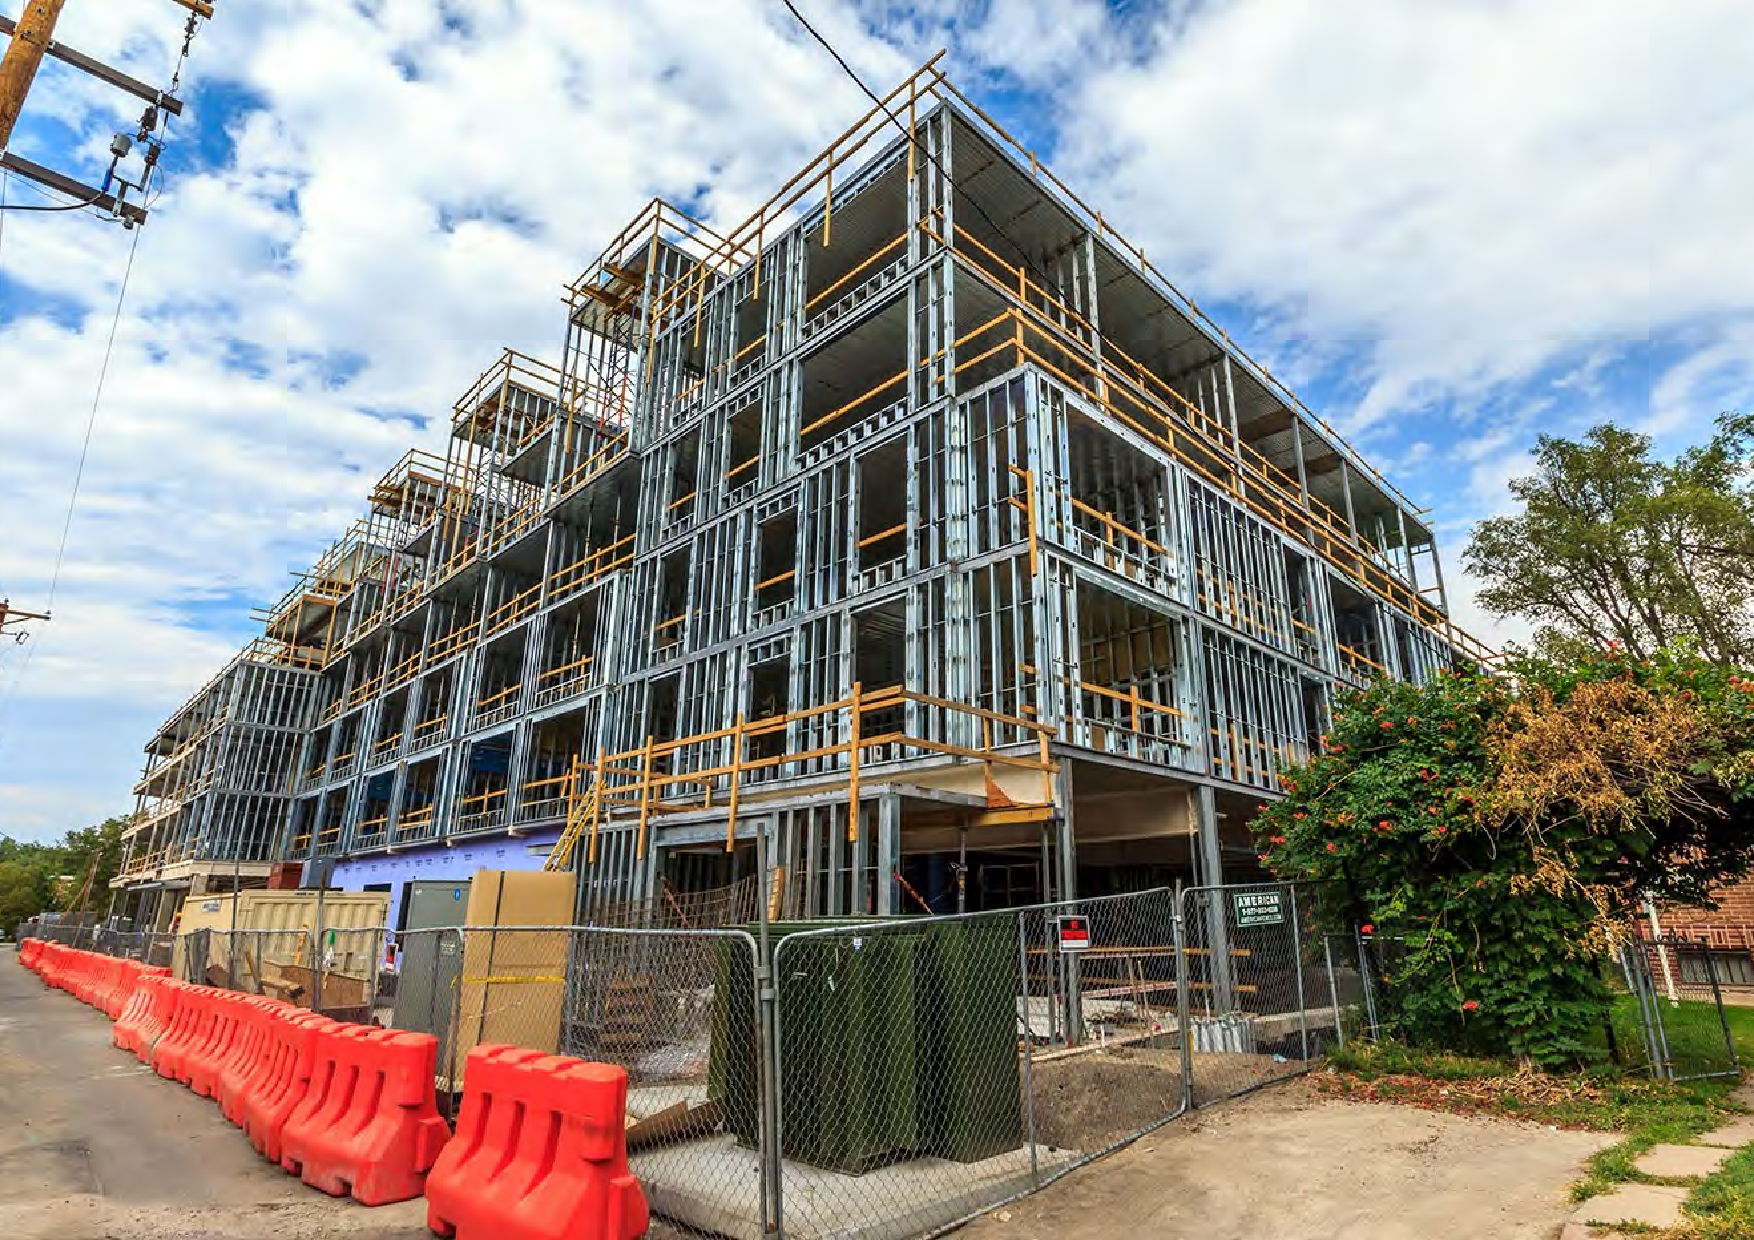
\includegraphics[width=7cm,height=5cm]{midrise1.pdf} &
			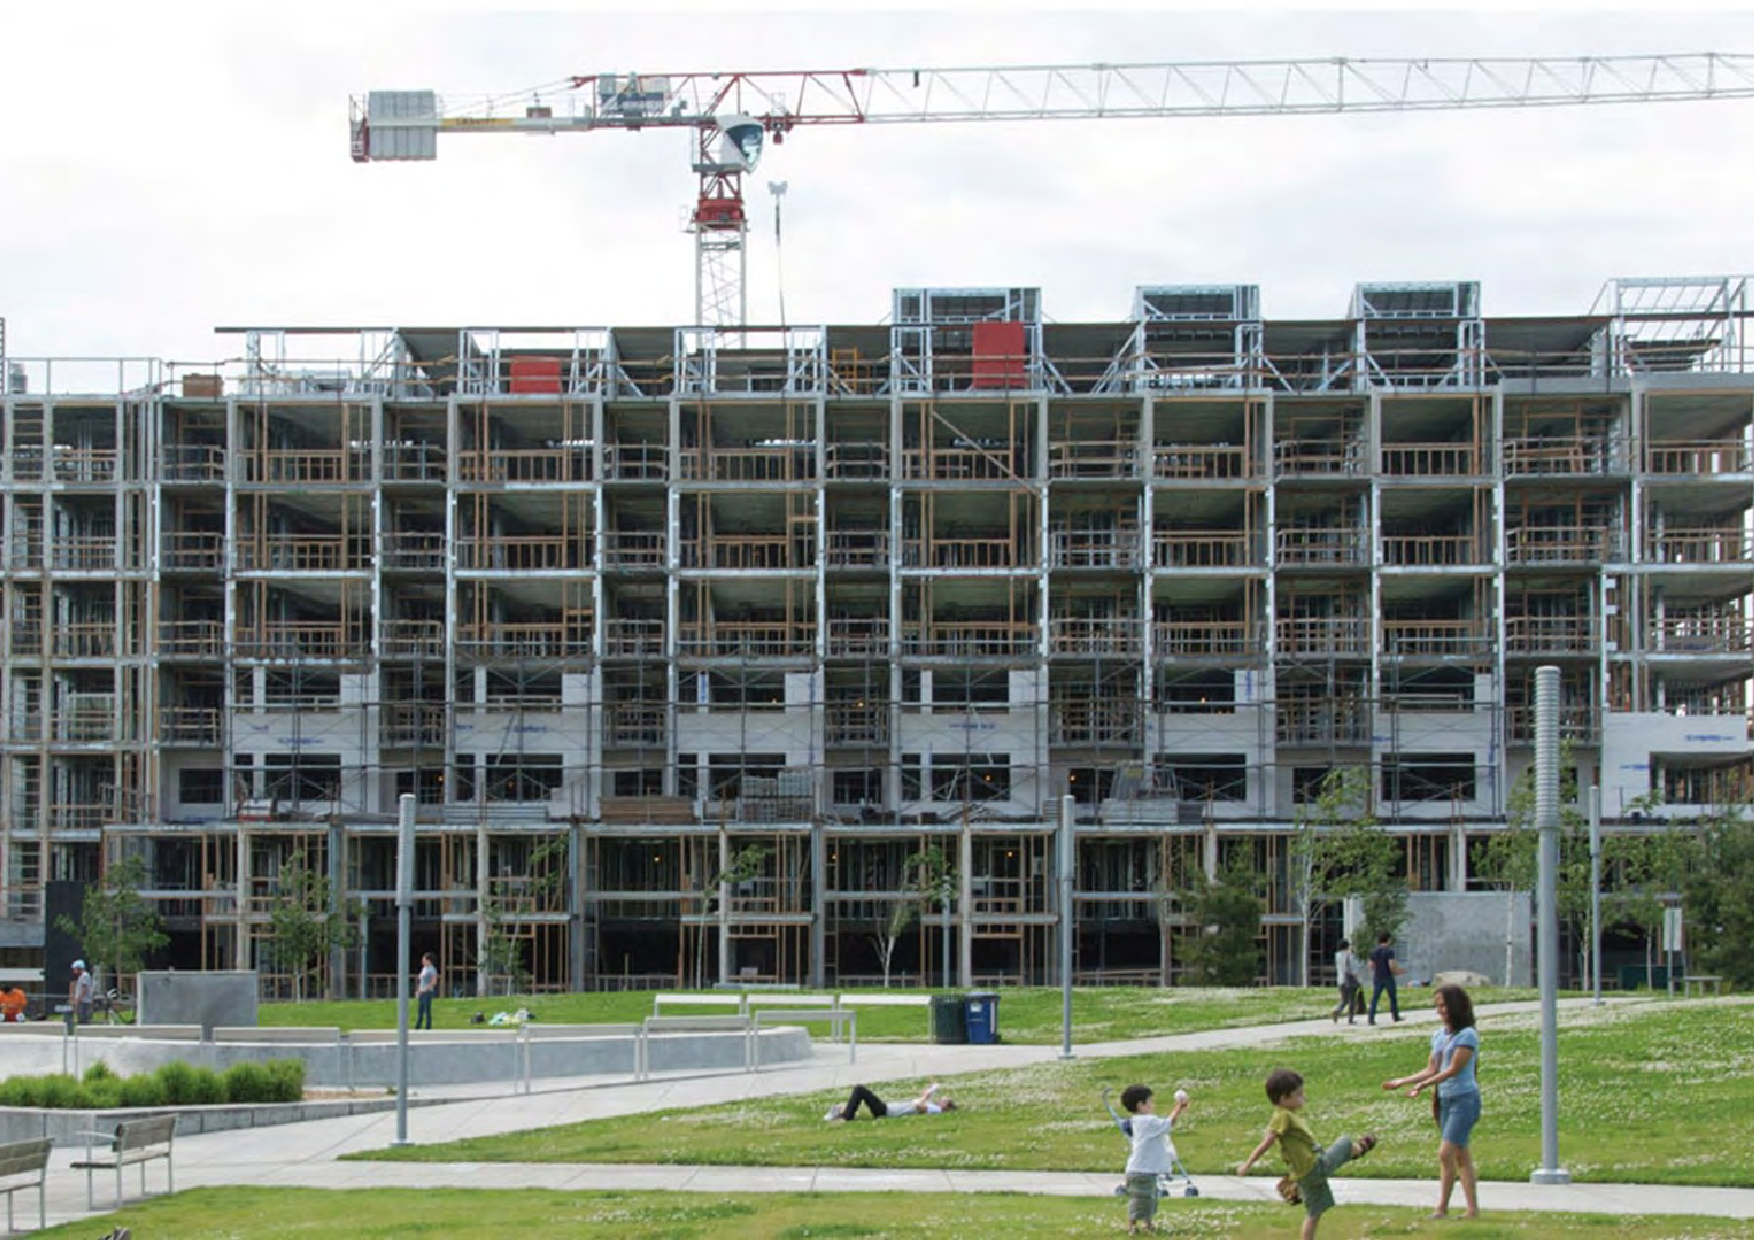
\includegraphics[width=7cm,height=5cm]{midrise2.pdf} \\
			(a) &
			(b) \\
		\end{tabular}
		\begin{scriptsize}
			Images extracted from (a) \url{https://starcash.co/steel-frame-building/astonishing-modular-products-prefabmarket/} (b) \url{https://ssfengineers.com/wp-content/uploads/2015/07/ballard-onthepark-b-copyright-bumgardner-architects-1920x1080.jpg}
			\end{scriptsize}	
		\caption{Mid-rise buildings with LSF wall system}
		\label{fig:midrise}
\end{figure}

\section{LSF Wall System}
\subsection{LSF Wall Components}

Light gauge steel frame / Lightweight steel frame wall systems are the latest advancements in modern wall construction. The main components of LSF wall systems include gypsum plasterboards, cold-formed steel sections (skeleton for the wall system), screws and other types of fasteners. The auxiliary components such as studs, tracks and noggings together form the skeleton of LSF wall system. The outer layer of the LSF wall system comprises of gypsum plasterboards. \Cref{fig:lsf_components} shows the components of a conventional LSF wall system based on a single row of studs in detail. The commonly used C-Section studs with double layers of plasterboard are shown in \Cref{fig:lsf_section}
\begin{figure}[htbp]
	\centering	
			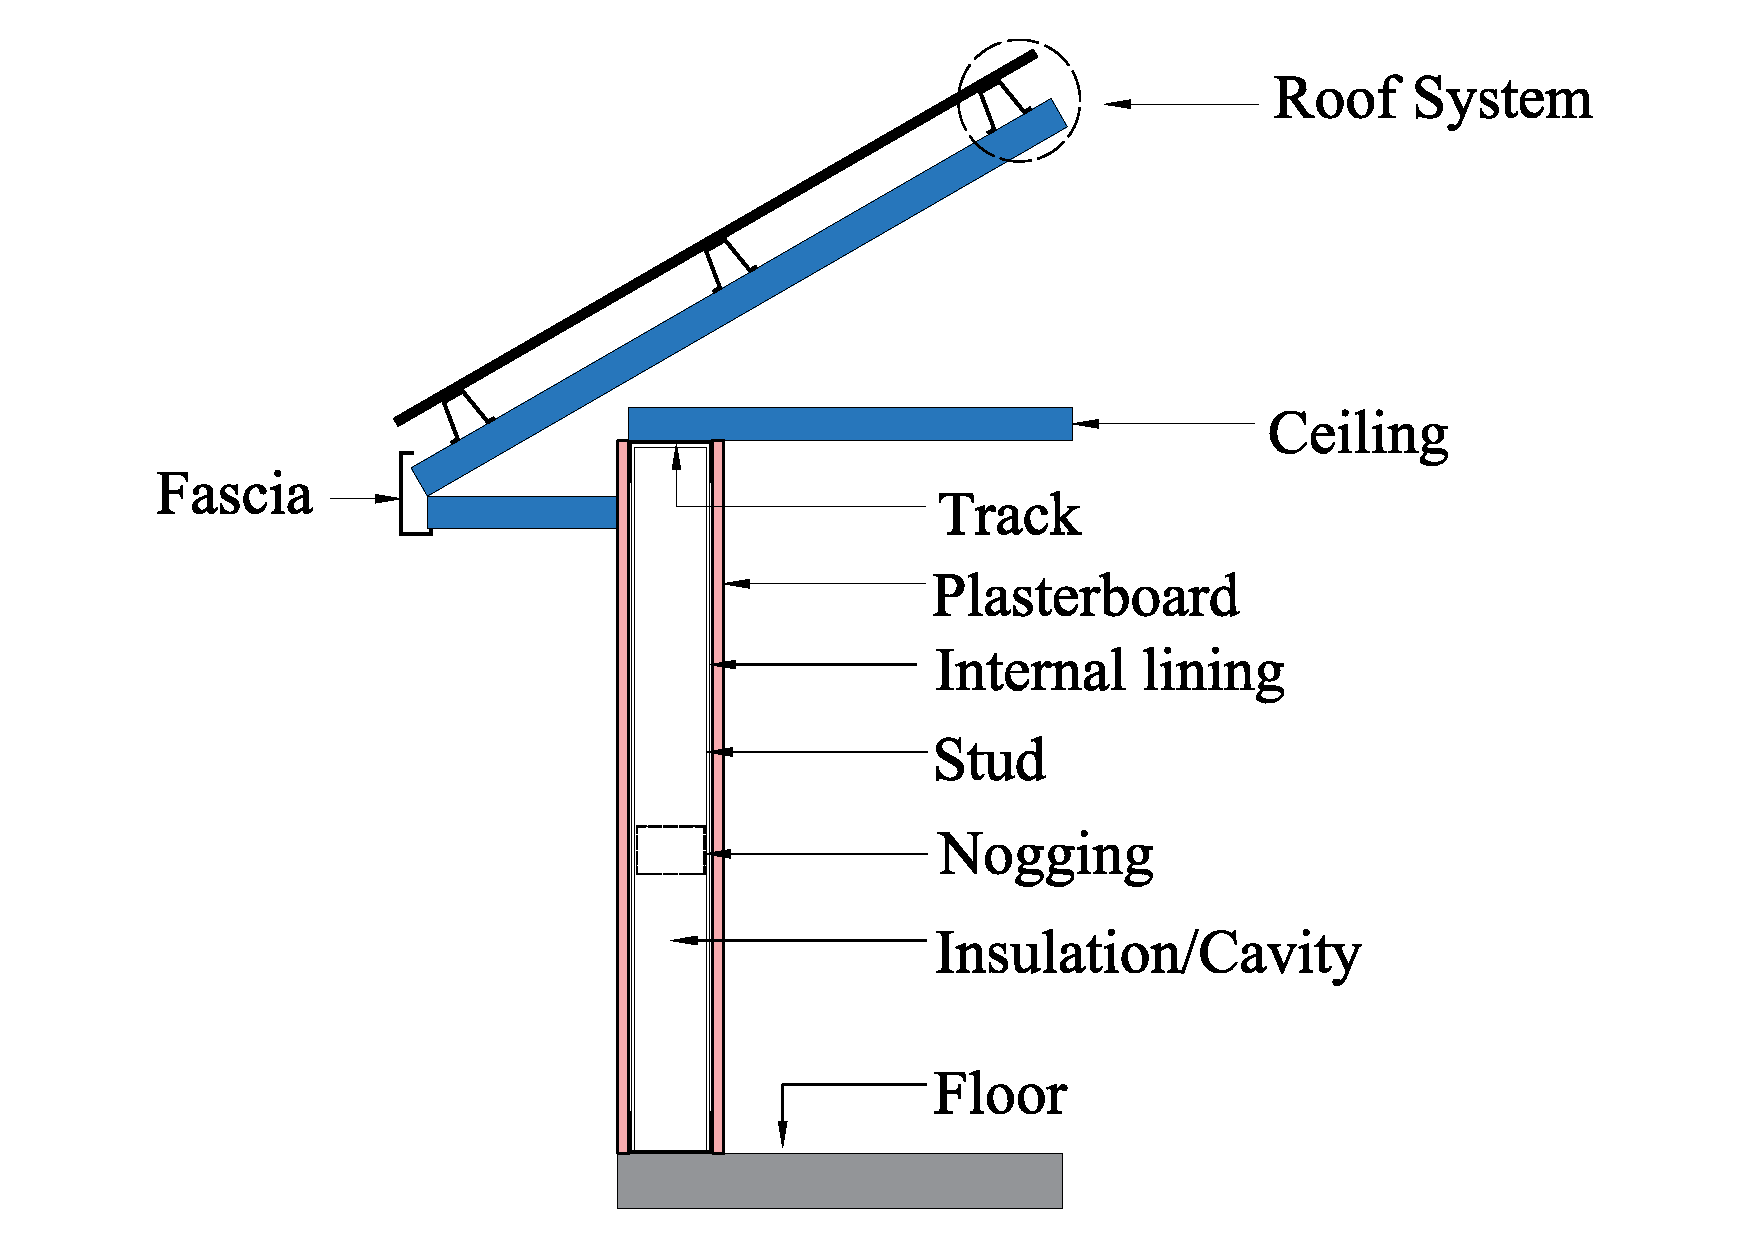
\includegraphics[width=9cm,height=7cm]{lsf_components.pdf}
				\caption{Components of LSF wall system}
		\label{fig:lsf_components}
\end{figure}
\begin{figure}[htbp]
	\centering	
		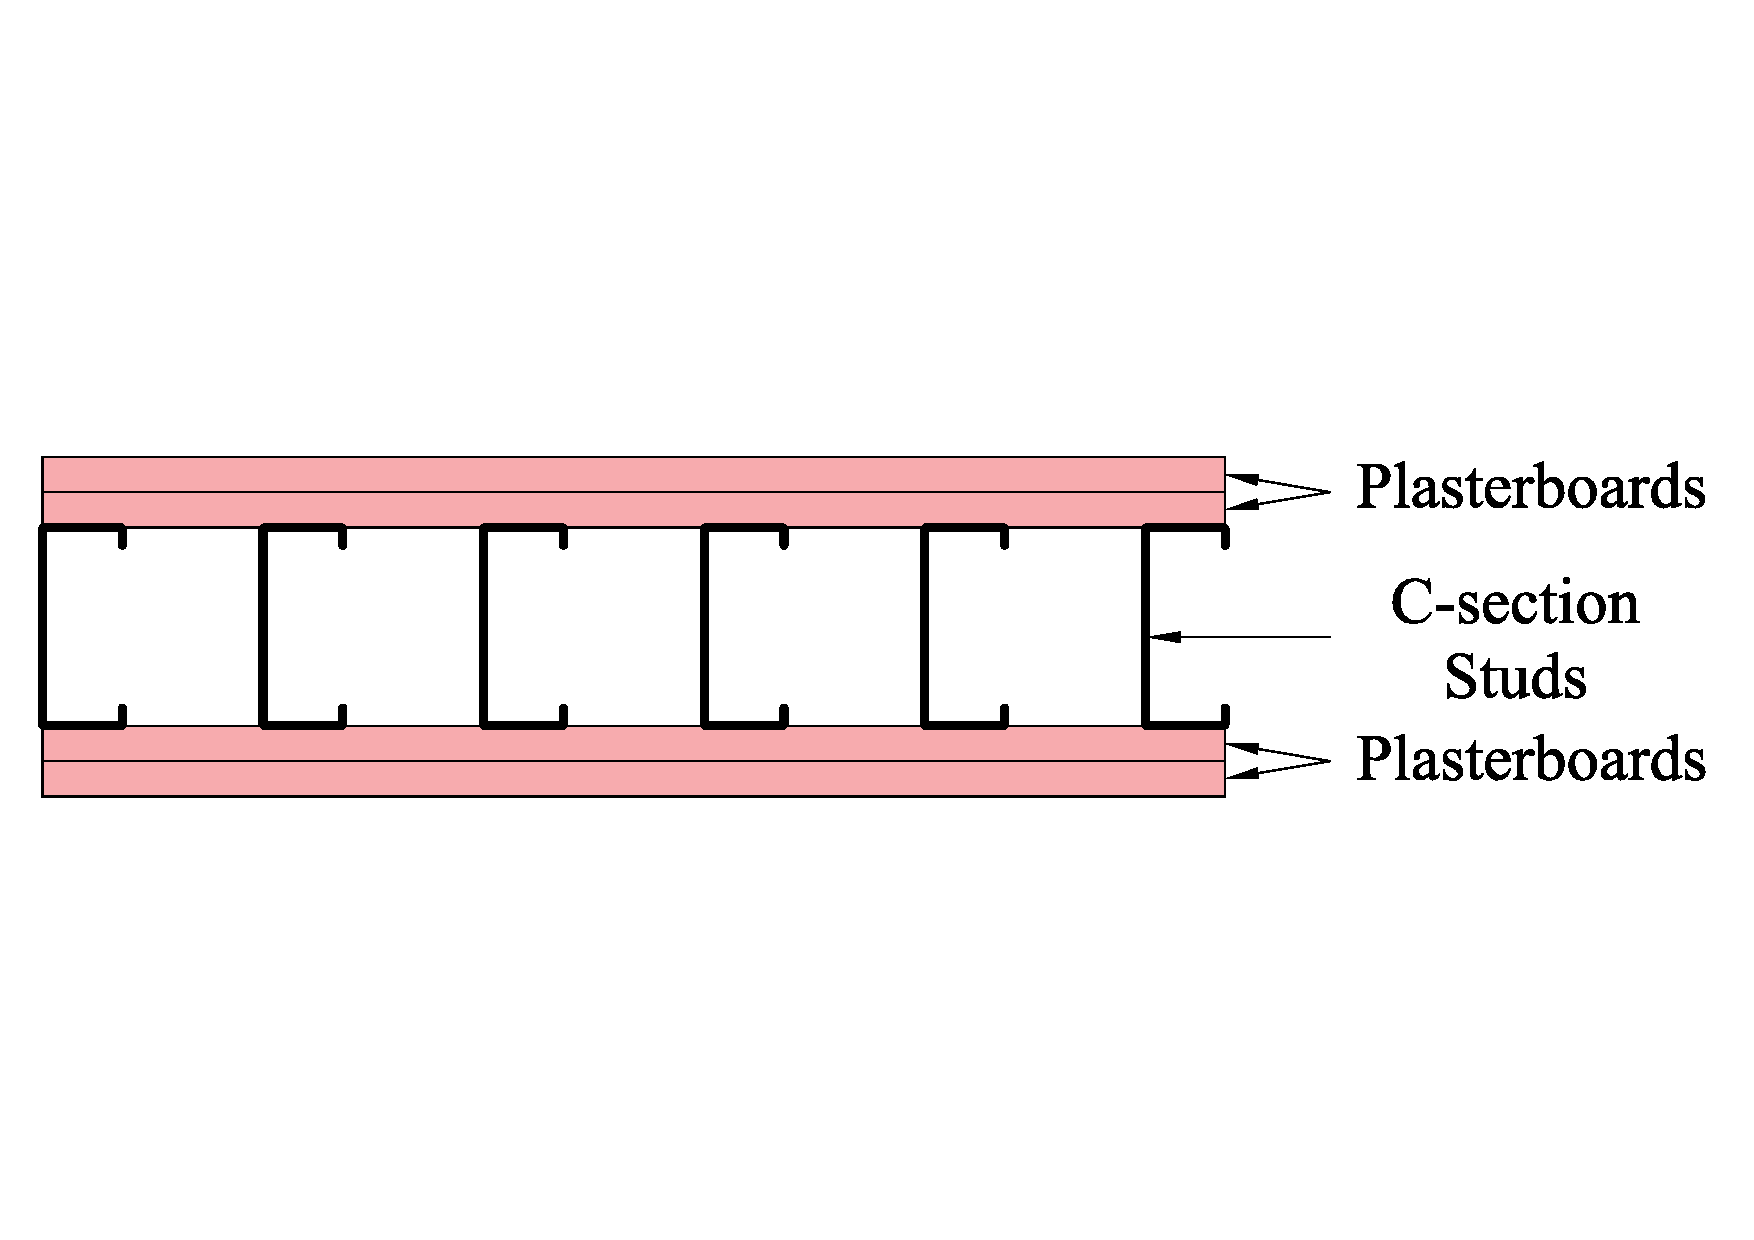
\includegraphics[width=10cm,height=2cm]{lsf_section.pdf}
		\caption{Plan view of LSF wall with Lipped C-Studs and double layers of plasterboard}
		\label{fig:lsf_section}
\end{figure}

In recent times, LSF wall, known as drywall, is an important constituent of modular building construction. Drywall also known as plasterboard are panel boards resembling plywoods and cardboards which are made of gypsum possessing the chemical name of Calcium sulphate dihydrate (CaSO4.2H2O). Plasterboards are manufactured by a process where the raw gypsum is dehydrated and then rehydrated to form calcium sulphate hemi hydrate. This is followed by mixing plaster with plasticizers and a foaming agent to achieve the necessary consistency. Ethelynediaminetetraacetic acid (EDTA) is used as a retardant in the manufacturing process to reduce the dew point, finally resulting in a pulp. This pulp is then sandwiched between two hard papers or fibre glass mats to form plasterboards. Some of the advantages of the plasterboard include ease of installation, thermal insulation, acoustic insulation and cost effectiveness.

Listed below are some of the advantages of LSF wall systems over conventional wall systems.

\begin{itemize}
\item Relatively low cost involved in the mass production of cold-formed steel sections.
\item Self-weight of the structure is less resulting in easier handling on site, minimizing the equipment handling cost.
\item Less time involved in constructing these walls in comparison with other wall systems.
\item Non-combustible in nature providing better fire resistance when compared to other wall systems as steel is the major component.
\item Better acoustic insulation as insulation layers can be customized within the wall panels as per end user requirement.
\item Eco-friendly construction as steel is the major component.
\item Resistance to termite attacks and weathering.
\end{itemize}

Even though the LSF wall systems possess many advantages, there are few areas in which the structural stability and strength of these wall systems can be compromised. One such area is the exposure of the LSF walls to elevated temperatures during fire exposure within or outside the building. Since steel is a good conductor of heat and the fact its mechanical properties deteriorate rapidly with increasing temperature, the cold-formed steel sections used within the LSF walls are vulnerable to both thermal and structural effects. Structural behaviour of LSF walls varies significantly at elevated temperatures when compared to ambient temperature conditions.

\subsection{Cold-formed Steel Sections}

Cold-formed steel sections are generally formed by cold pressing of thin steel sheets to the desired shape and size at ambient temperatures. Stamping and rolling methods are also employed for manufacturing some of the cold-formed steel sections. Cold-formed steel sections are generally designated as Channel/C-sections, Lipped channels, Nested Channels, I-sections, RHS (Rectangular Hollow Sections), CHS (Circular Hollow Sections), SHS (Square Hollow Sections), RHFCB (Riveted Hollow Flange Channel Beam) sections and Built-Up sections. Typical cold-formed steel sections are shown in \Cref{fig:typical_section}. Unlike the manufacturing process of hot-rolled steel sections, where the rolling of steel takes place at a very high temperature of 1700 \degree F (greater than the recrystallization temperature of steel), cold-formed steel sections are manufactured at room temperature.
\begin{figure}[htbp]
	\centering	
		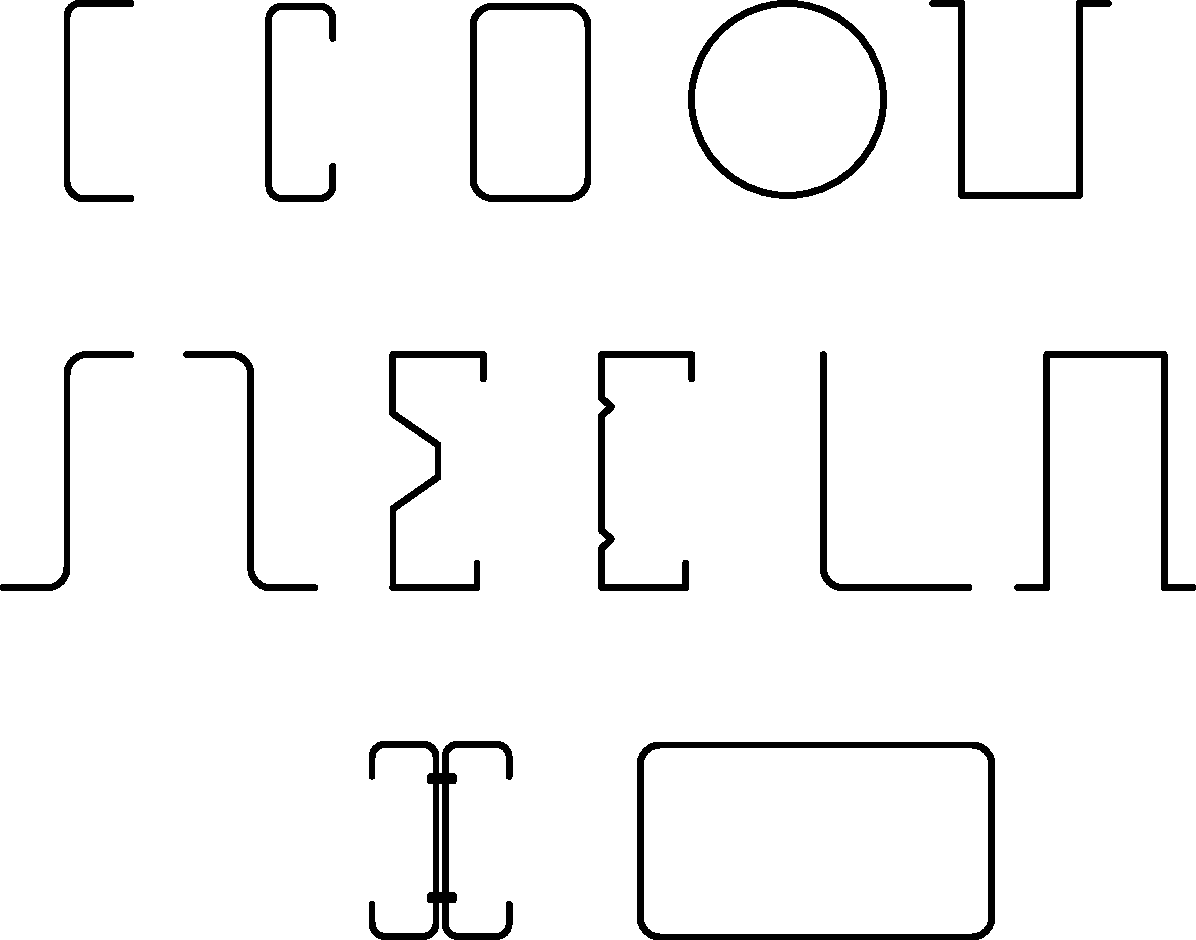
\includegraphics[width=7cm,height=5cm]{typical_sections.pdf}
		\caption{Typical Cold-Formed Steel Sections (CFS)}
		\label{fig:typical_section}
\end{figure}

Cold-formed steel can be termed as a derivative of hot-rolled steel as it is hot-rolled steel with further processing with a better surface finish than hot-rolled steel. The manufacturing process generally involves cold drawing, turning, grinding, polishing to get a smoother finish when compared to hot-rolled steel.

\subsection{Buckling Behaviour of Cold-Formed Steel Members}

As the name suggests, cold-formed steel sections are thin and their thickness varies from 0.55 mm to 8 mm. The thickness of cold-formed steel section is small in comparison with its width and thus local buckling of flanges/web will occur before section yielding. However, local buckling of the section does not imply that the section has reached its ultimate capacity. This phenomenon is referred to as post-buckling strength. Local buckling takes place at low compressive stresses as the width to thickness ratio is high in cold-formed steel sections.

The structural behaviour of cold-formed steel sections varies when compared to hot-rolled steel sections. This behaviour change is noticeable not only at ambient temperatures, but also at elevated temperatures. For instance, the plate and column slenderness ratios of cold-formed steel columns are higher than those of hot-rolled steel columns. This results in increased local and global buckling effects when compared to hot-rolled steel section columns. These effects can worsen at elevated temperatures. \Cref{fig:buckling_modes} shows the different types of buckling modes of a cold-formed steel column while \Cref{fig:buckling_plot} shows the corresponding buckling curve/plot. 
\begin{figure}[htbp]
	\centering	
		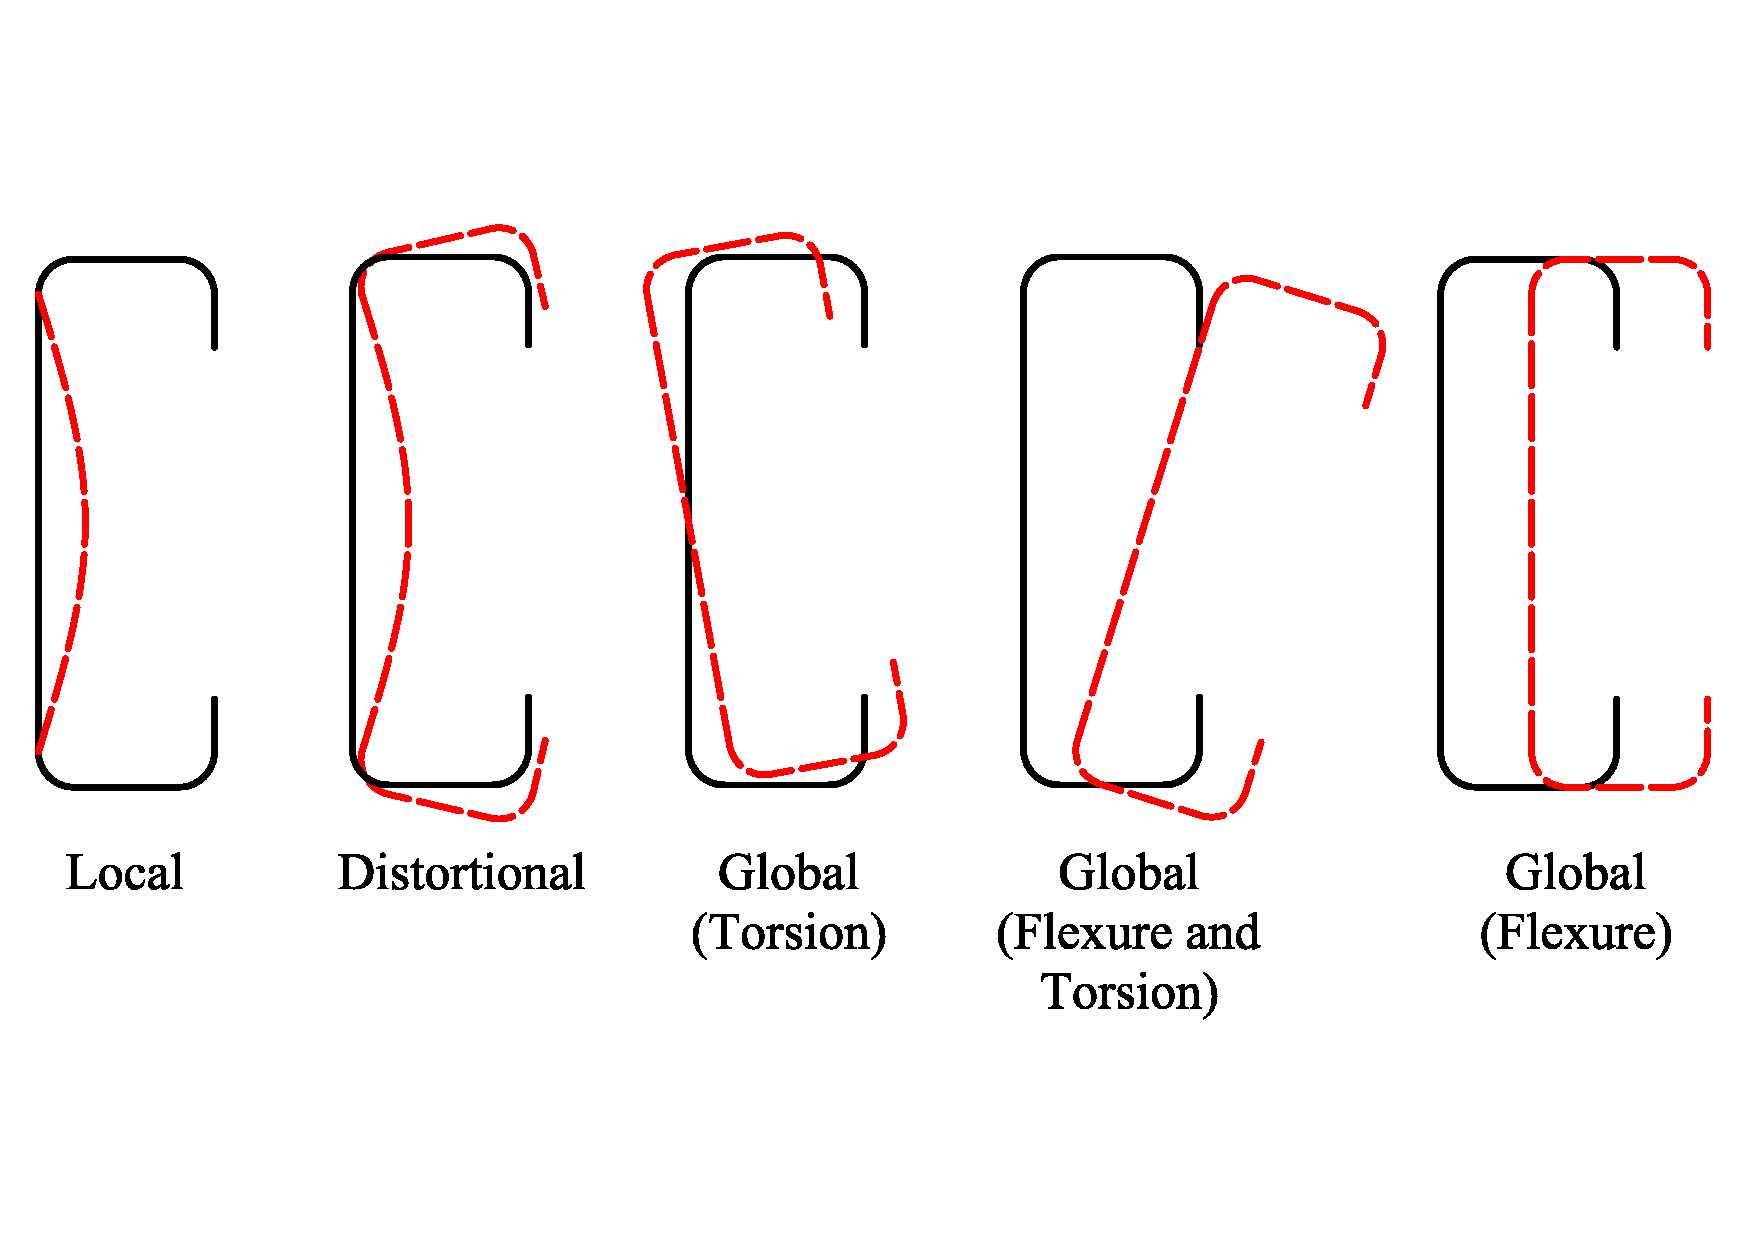
\includegraphics[width=8cm,height=3.5cm]{buckling_modes.pdf}
		\caption{Different buckling modes of a channel section column}
		\label{fig:buckling_modes}
\end{figure}
\begin{figure}[htbp]
	\centering	
		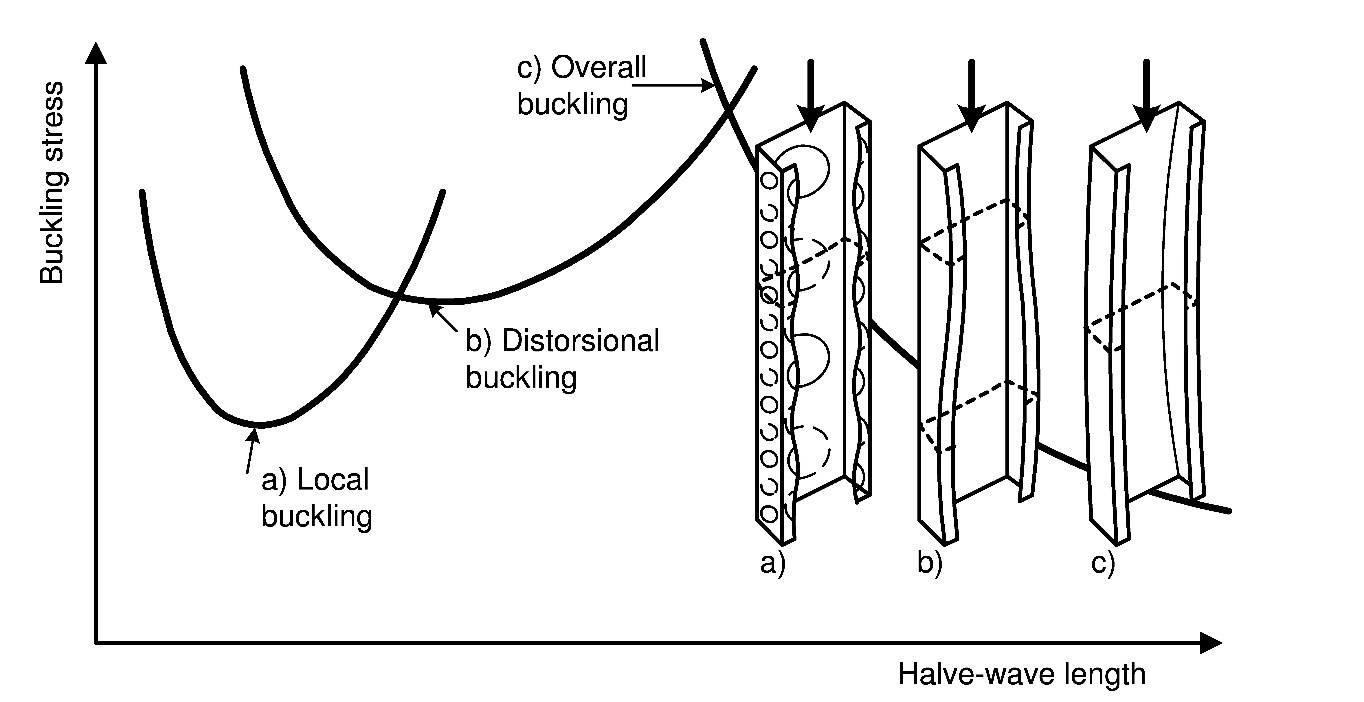
\includegraphics[width=8cm,height=4cm]{buckling_plot.jpg}
		\caption{Buckling plot from BS EN 1993-1-3 (2005a)}
		\label{fig:buckling_plot}
\end{figure}

\subsection{Design Guidelines}

The design standard pertaining to the structural design of cold-formed steel sections in Australia is AS/NZS 4600 (2014). Other design standards generally used in the cold-formed steel member design are AISI S100-12 ( 2007), AISI S202-15 and EN 1993-1-3:2006, which  provide the ambient temperature capacity equations for cold-formed steel members subjected to various actions such as compression, bending and their combinations. In the capacity calculations, the yield stress is taken as 0.2\% proof stress. When cold-formed steel members are exposed to fire conditions, specific design capacity equations are needed to predict the capacity deterioration due to fire. EN 1993-1-2 provides appropriate fire design rules, but they were mostly developed to suit hot-rolled steel members. Recent research by \citet{Ranawaka2009a}, \citet{Kankanamge2011} and \citet{Rokilan2019} have therefore focused on the behaviour and capacity determination of cold-formed steel members at elevated temperatures.

\subsection{Fire and Structural Performance of LSF walls}

Fire resistance level is used in the construction industry to determine the resistance to failure offered by structural components of a building in fire. This grading is designated in minutes under the following three criteria by NCC (2016).

\begin{itemize}
\item Structural adequacy - the ability to maintain adequate stability in fire.
\item Integrity - the ability to resist the passage of wall flames and fumes from the fire-exposed face of the wall to the unexposed face. 
\item Insulation - the ability to maintain a temperature on the surface of the unexposed face of the system to the limits specified as in AS/NZS 1530.4:2014 (SA, 2014).
\end{itemize}

The limiting values for the structural adequacy, integrity and insulation are specified in  NCC for various structural systems. The fire resistance level of an LSF wall is generally given in minutes (or hours) for each of the three criteria above.

Fire resistance of LSF walls is dependant on the thermal properties of the materials used in the wall system such as thermal conductivity, specific heat and relative density. \citet{Keerthan2012} investigated the thermal properties of gypsum plasterboards under standard fire conditions and provided a set of the thermal properties for use in the numerical models for validation purposes. The proposed thermal properties were also compared with the experimental fire test results of plasterboards and were observed to have good correlation. Cold-formed steel sections are often point symmetric, mono symmetric or non-symmetric, i.e. not doubly symmetric as shown in \Cref{fig:symmetry}. 
\begin{figure}[!htbp]
	\centering
		\begin{tabular}{cc}
			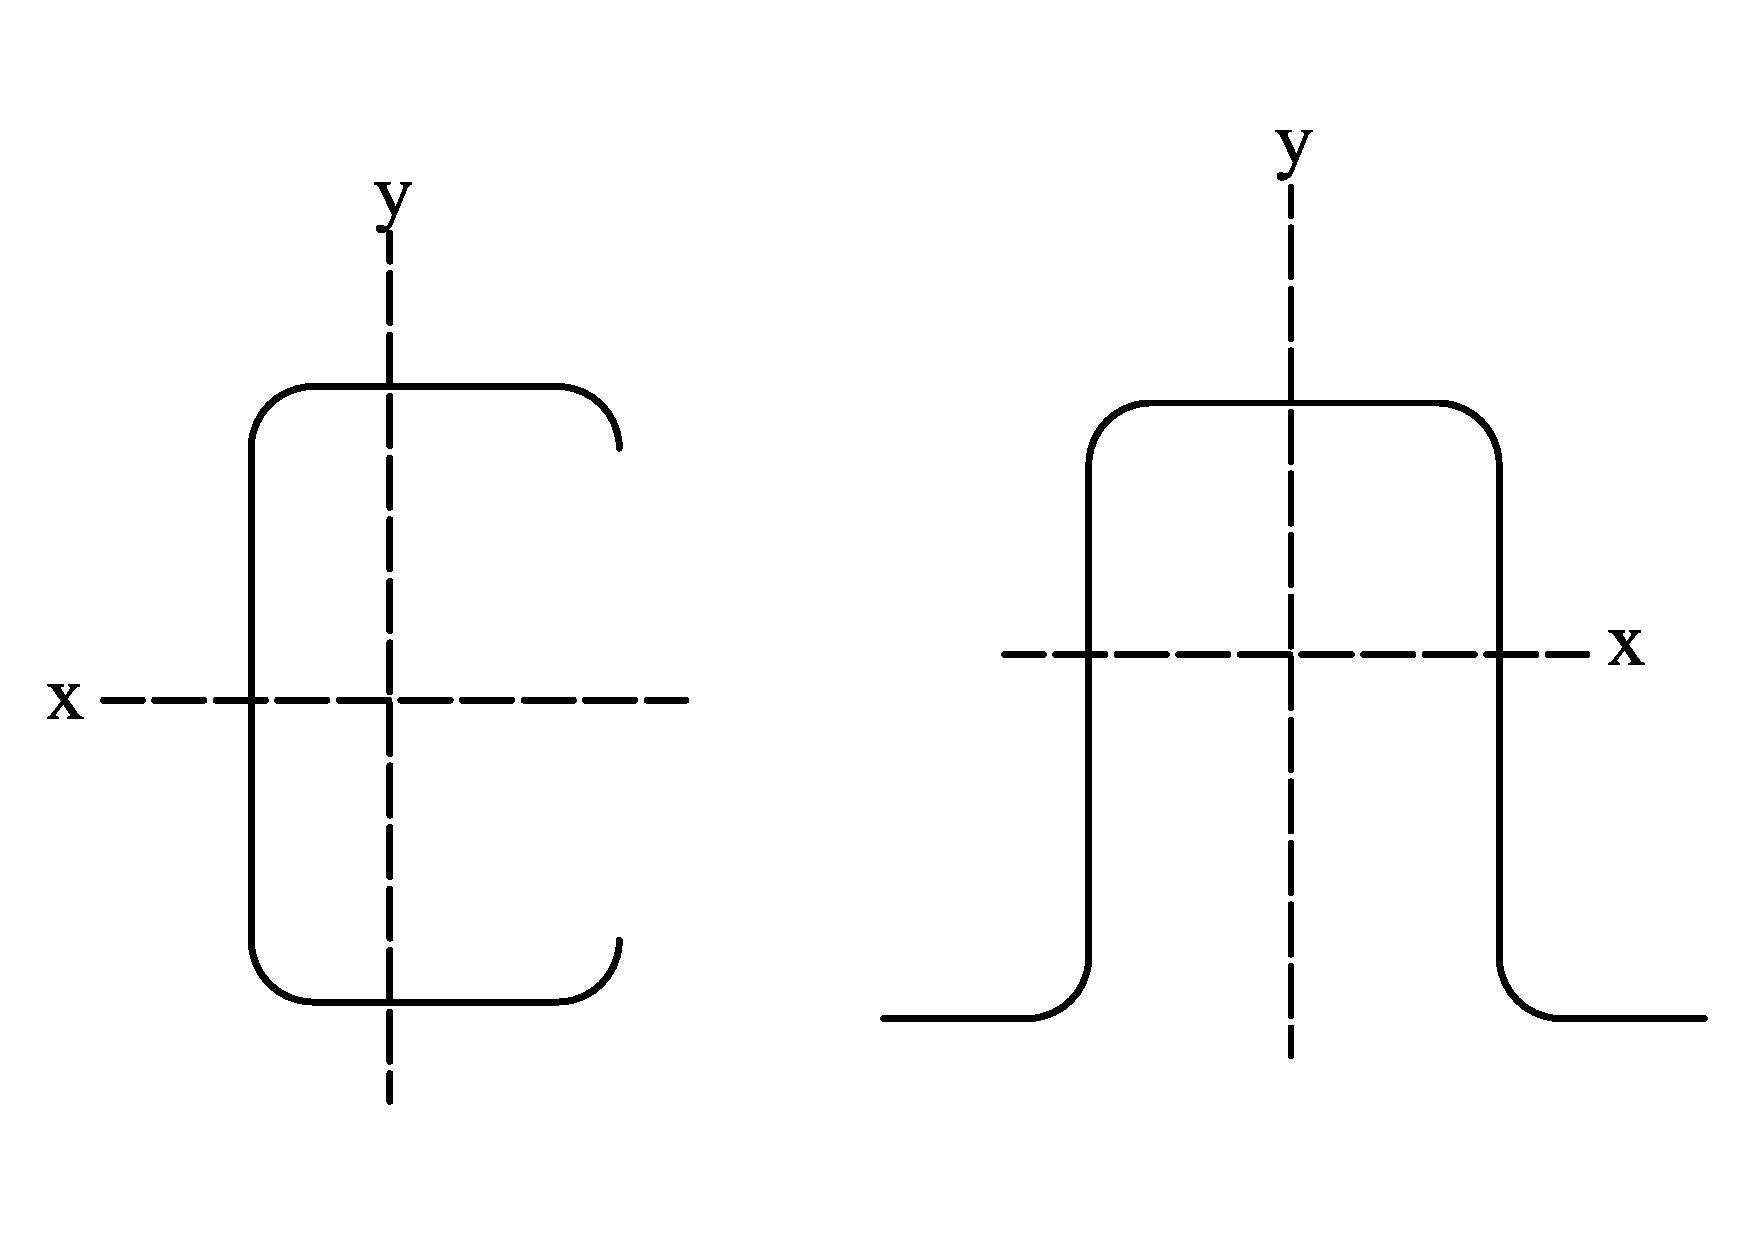
\includegraphics[scale=0.15]{singly_symmetric} & 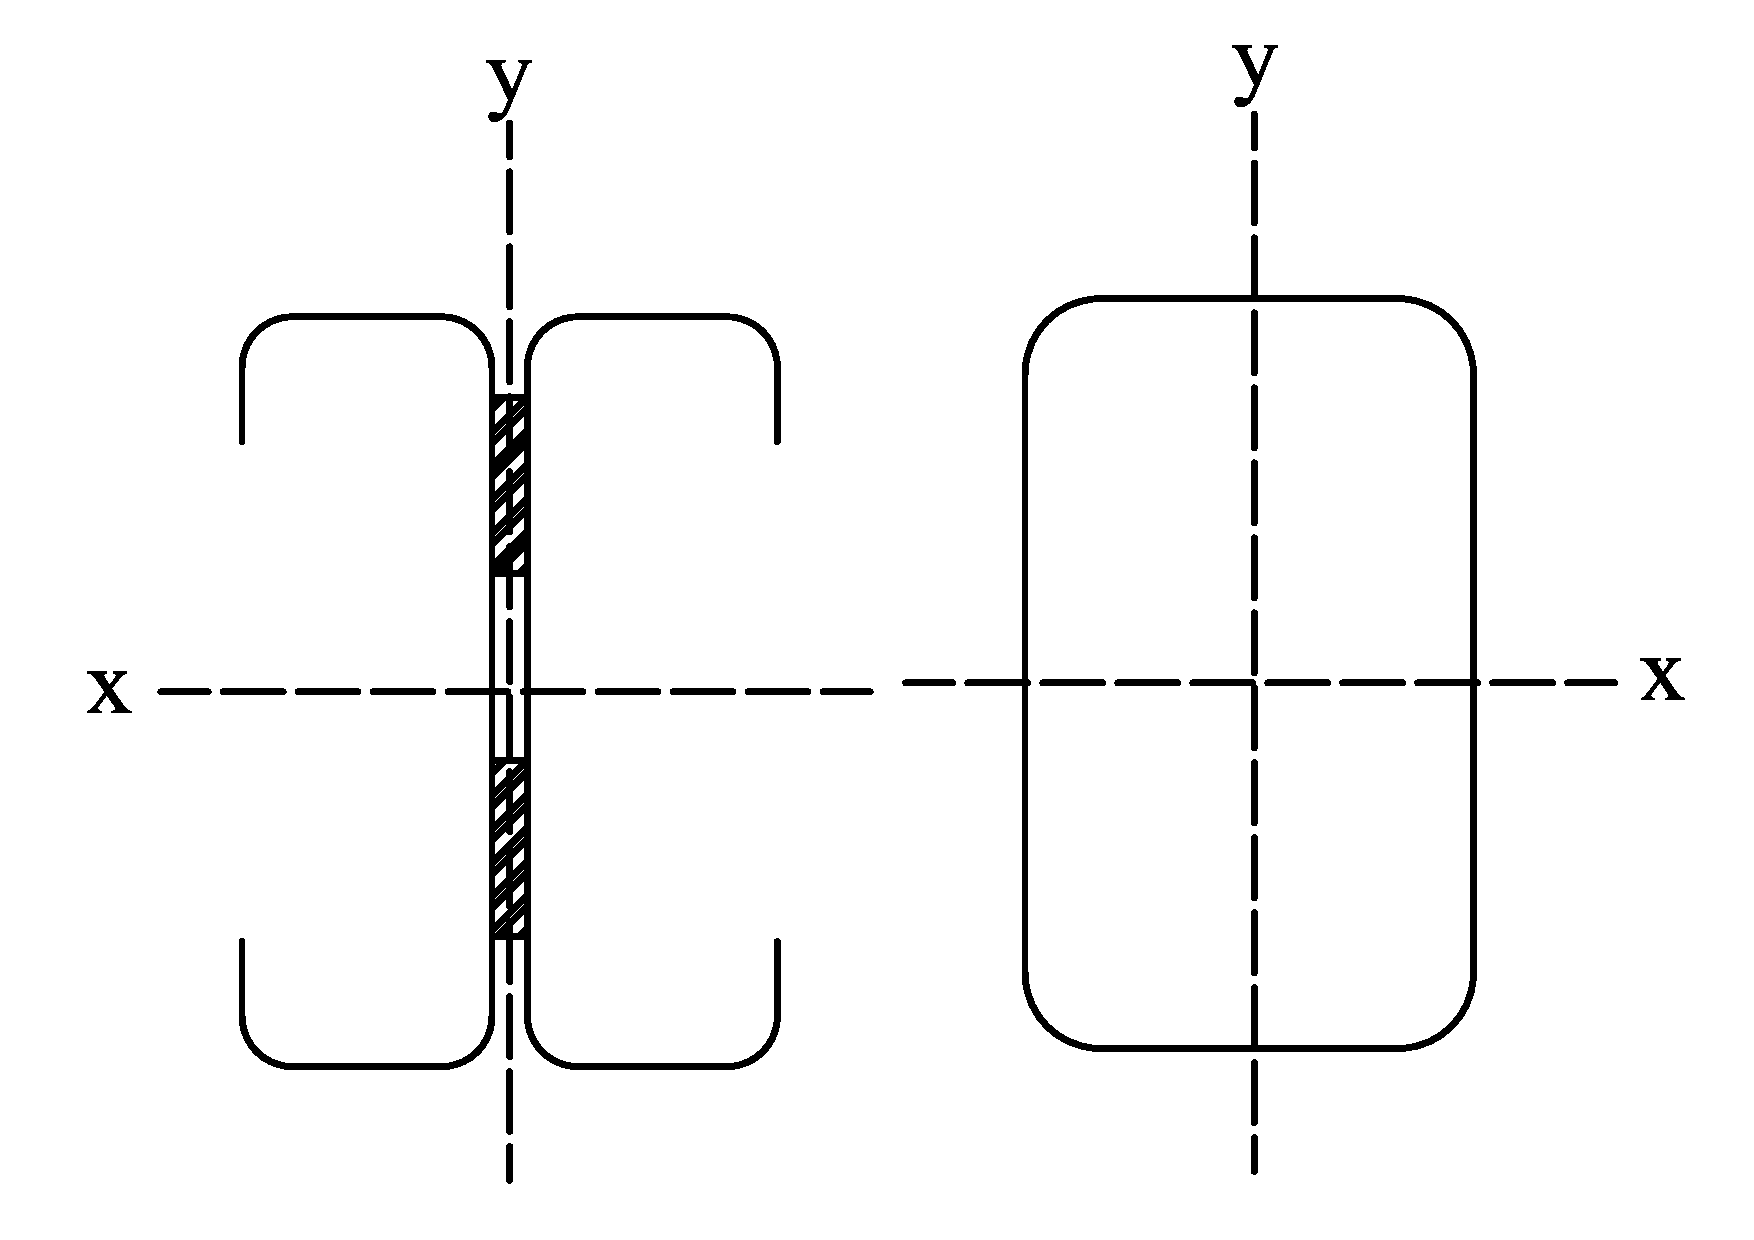
\includegraphics[scale=0.15]{doubly_symmetric} \\ 
			(a) & (b)  \\ 
			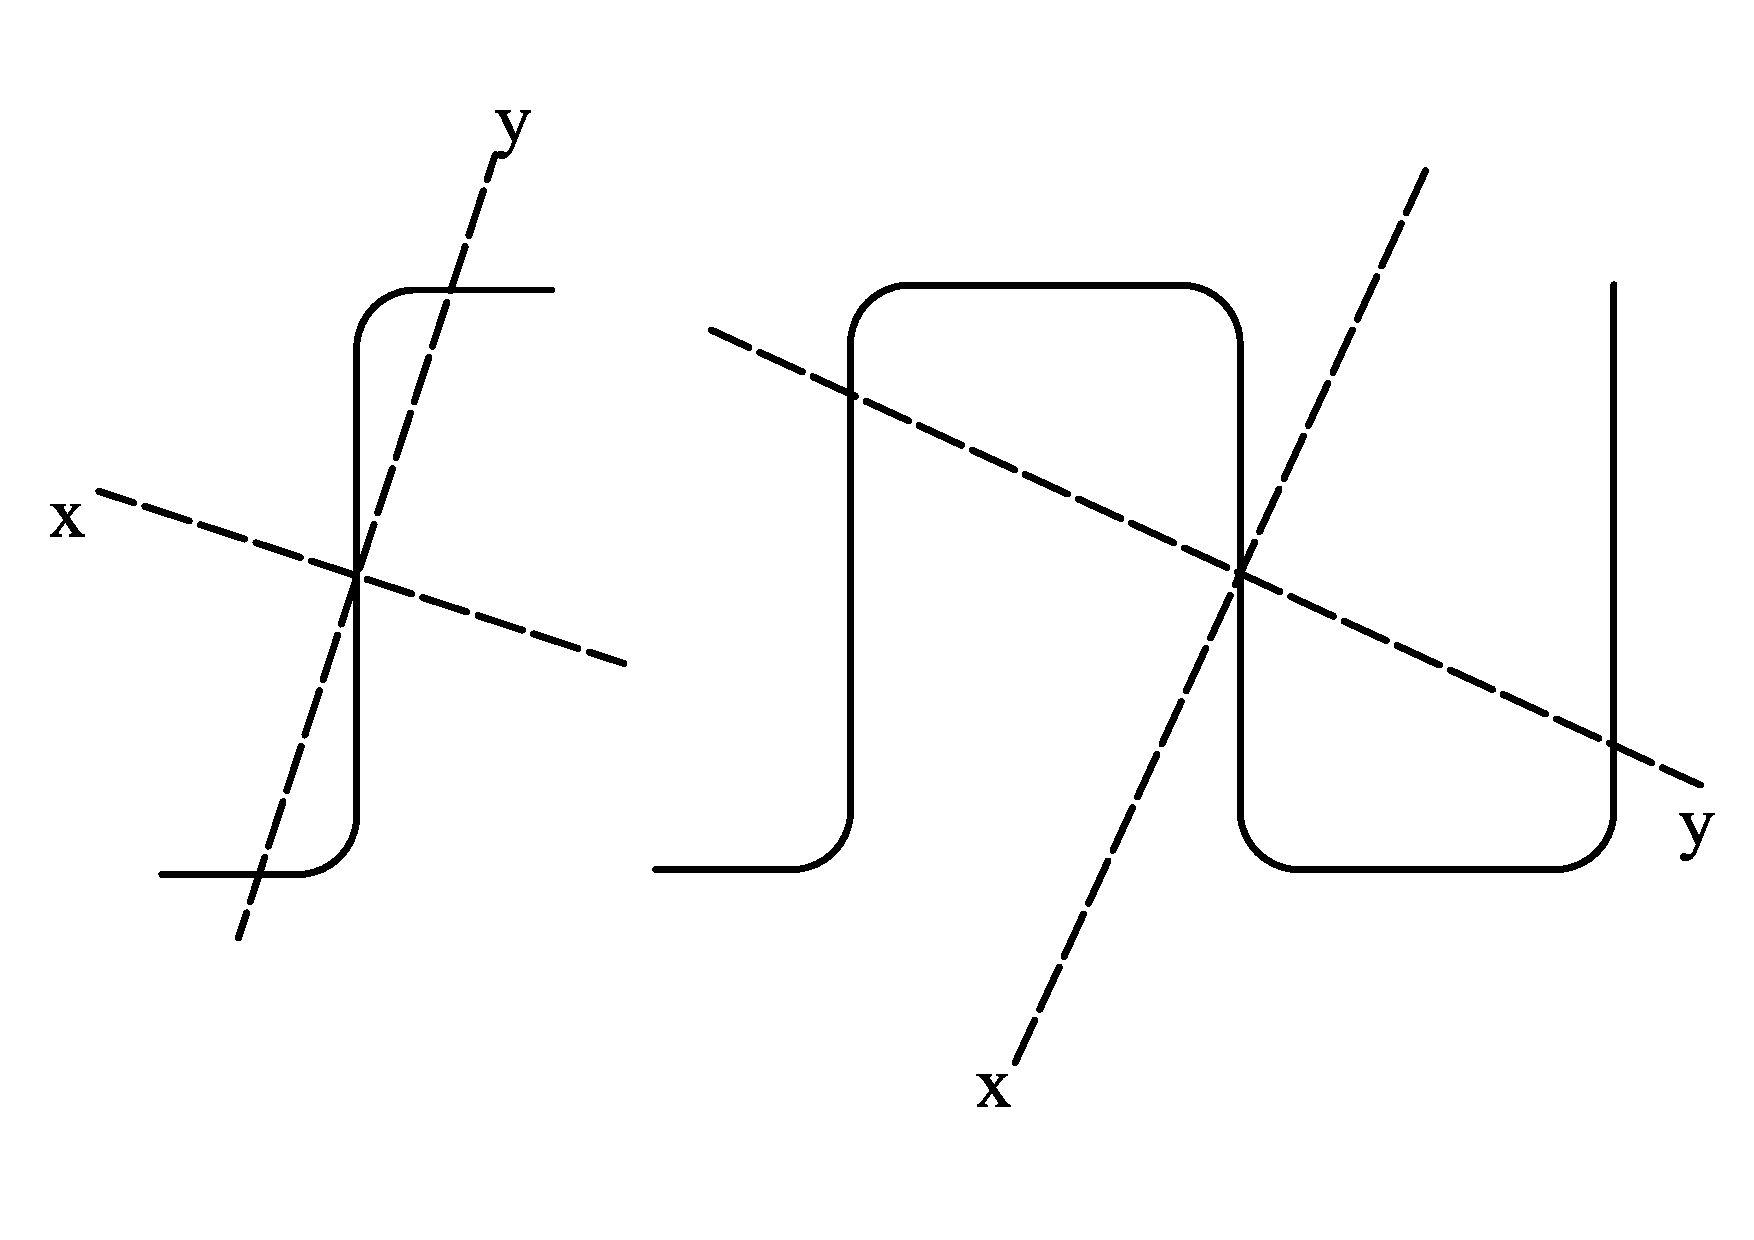
\includegraphics[scale=0.15]{point_symmetric} & 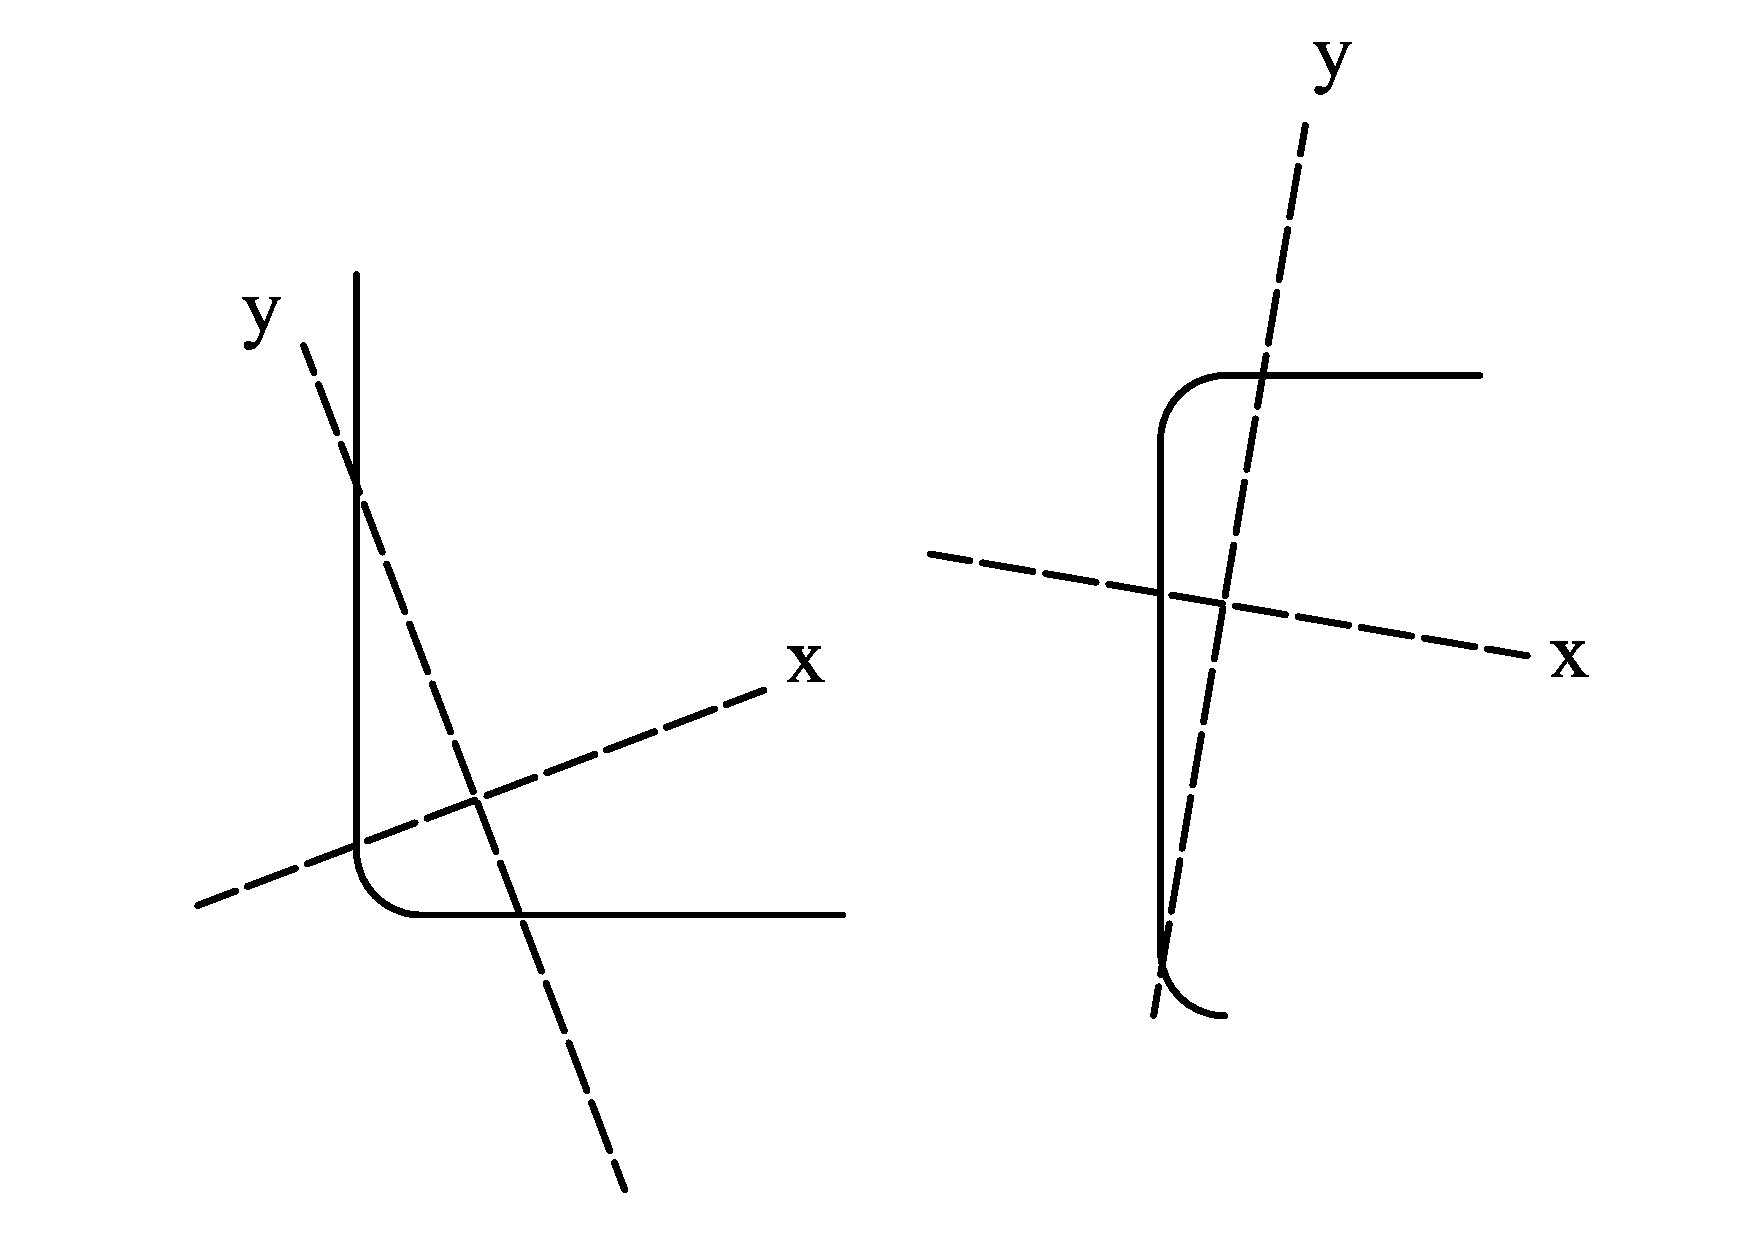
\includegraphics[scale=0.15]{non_symmetric} \\ 
			(c) & (d)  \\
		\end{tabular} 
		\caption{Different types of symmetric sections(a) Singly (b) Doubly (c) Point (d) Mono}
		\label{fig:symmetry}
\end{figure}
Hence, they are subjected to more complex buckling modes. When the mono-symmetric lipped channel studs are exposed to fire on one side, they are subjected to the following
\begin{itemize}
	\item Temperature gradient across the depth resulting in thermal bowing.
	\item Non-uniform mechanical properties across the cross-section as the hot flange mechanical properties are much less than those of cold flange.
\end{itemize}
\begin{figure}[htbp]
	\centering	
		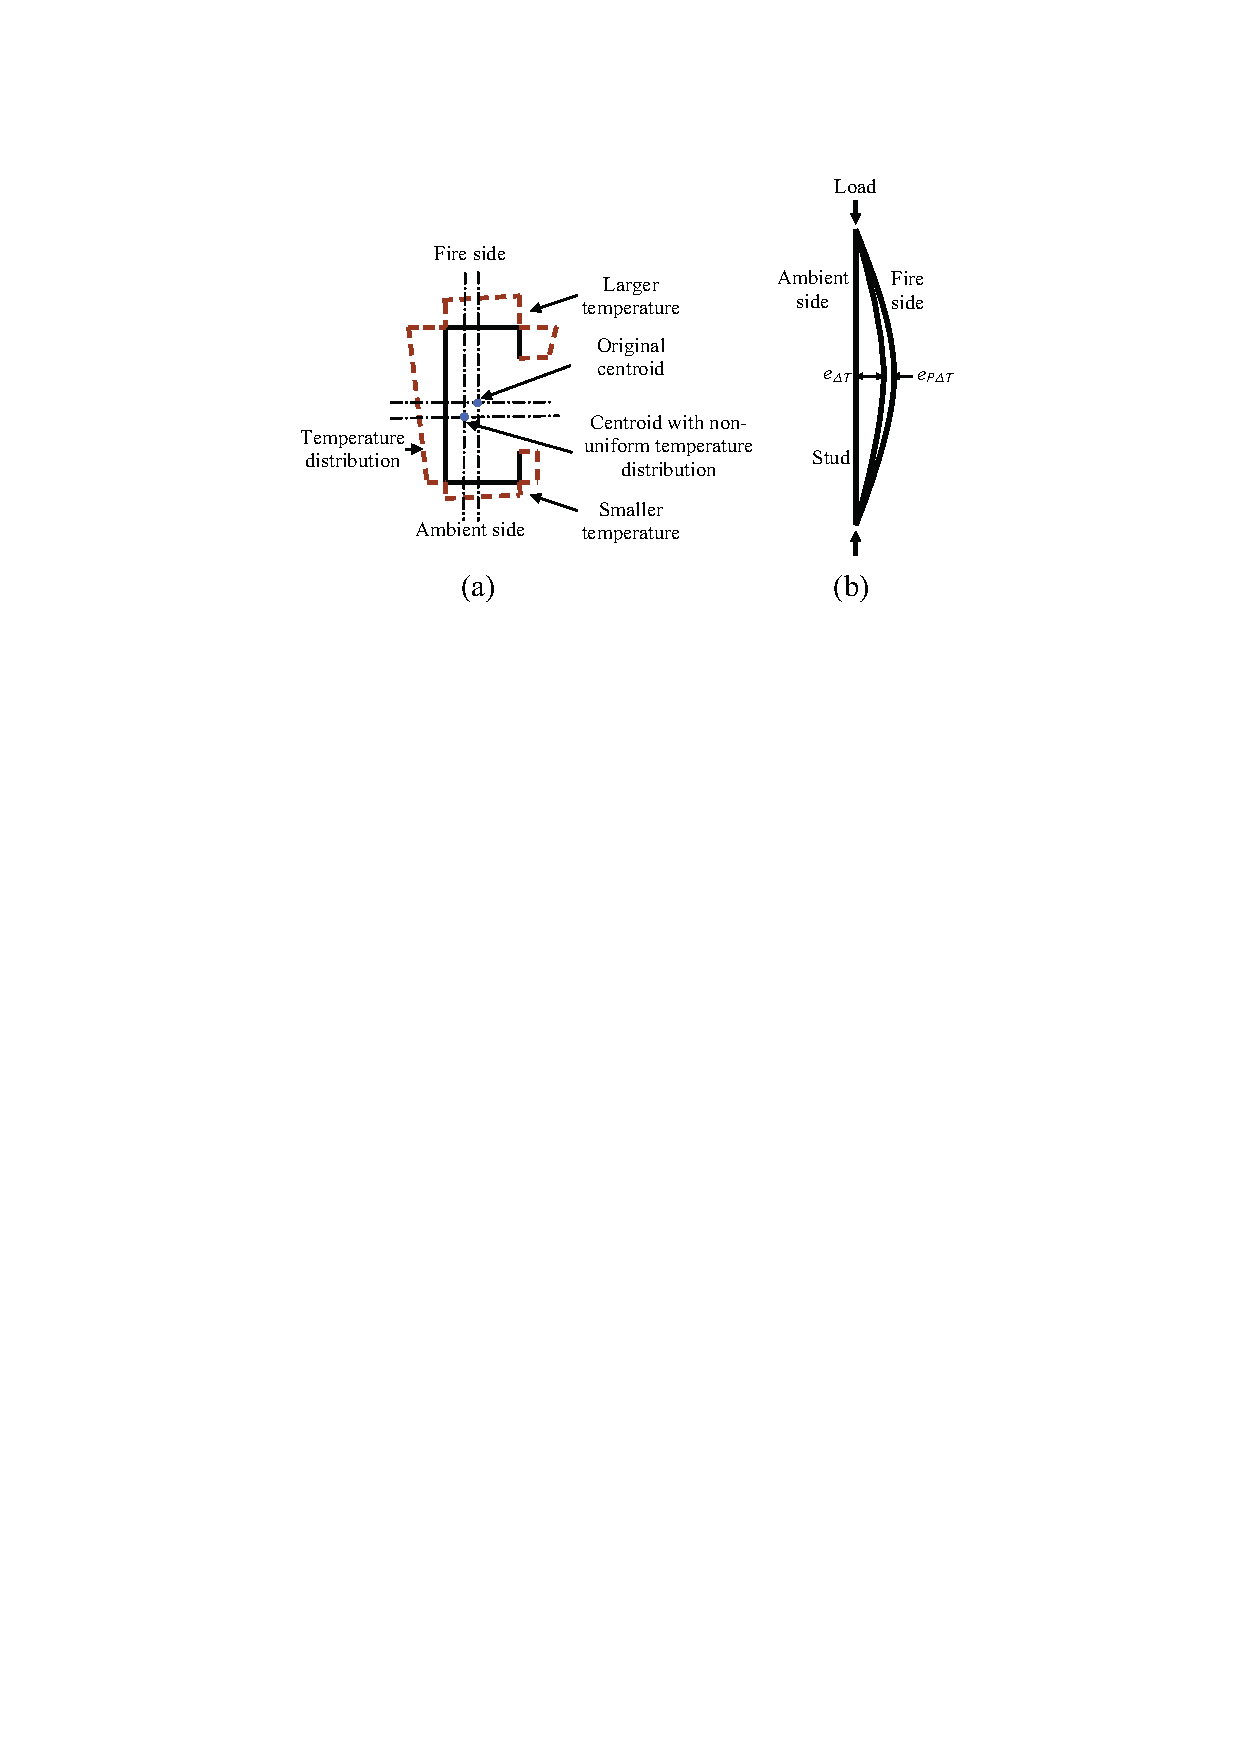
\includegraphics[width=8cm,height=5cm]{gunalan_nutemp}
		\caption{Neutral axis shift due to thermal bowing (\cite{Gunalan2014j})}
		\label{fig:gunalan_nutemp}
\end{figure}
\begin{figure}[htbp]
	\centering	
		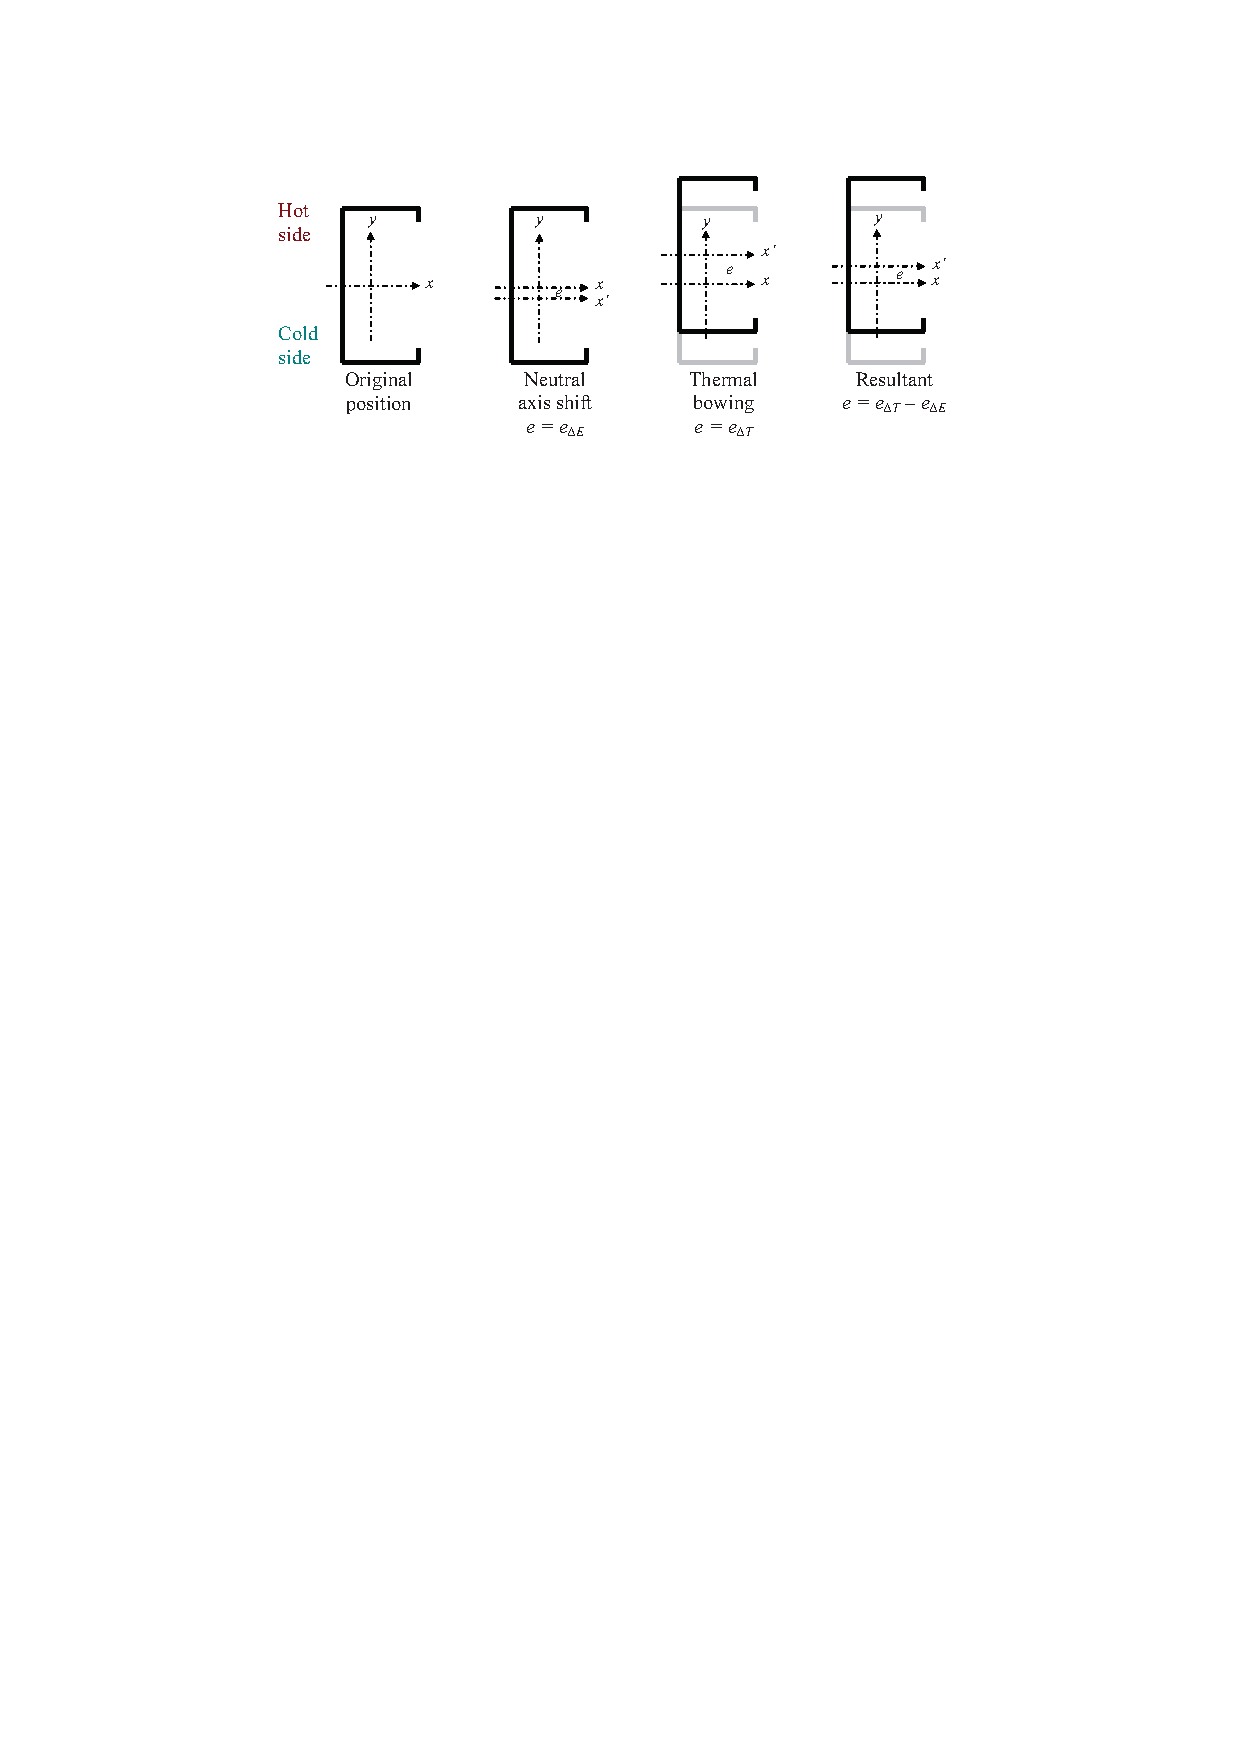
\includegraphics[width=8cm,height=4cm]{gunalan_nashift}
		\caption{Lateral deflection due to thermal bowing (\cite{Gunalan2014j})}
		\label{fig:gunalan_nashift}
\end{figure}
The presence of non-uniform mechanical properties leads to neutral axis shift of the stud section (\Cref{fig:gunalan_nutemp,fig:gunalan_nashift}). These actions caused by fire exposure on one side induce the thin-walled stud to be subjected to a bending moment in addition to the applied axial compression load.

\section{Complex LSF Wall Systems}
Complex LSF wall systems are needed and are being used in various applications in the building sector. Some of these wall systems are based on double and staggered stud configurations Figures \ref{fig:typical-complex}~(a) to (c). To withstand heavy structural loads in the case of mid-rise construction, such systems are preferred. Also, to achieve higher acoustic insulation in places where sound insulation is important, these wall systems are used. Double stud walls are those with two parallel rows of studs with studs located directly opposite to each other whereas studs in parallel rows are staggered in case of staggered stud walls. Lipped channel steel sections are widely used as the studs in LSF walls. The major components of the double and staggered stud walls include two rows of cold-formed steel studs, tracks, noggings, bracings, and plasterboards. These components are fixed together using self-piercing screws of different types. The physical and thermal properties of the double and staggered stud wall components are similar to single stud LSF walls. But due to the increased cavity depth, the behaviour of the components such as studs under fire exposure is different. The acoustic, thermal and structural performance of double and staggered stud walls is likely to be superior compared to single stud walls. Plasterboard manufacturers such as USG Boral, CSR and Knauf Plasterboard include double and staggered stud wall systems in their product manuals although their main focus is on double stud wall systems. To date no detailed research has been undertaken on the thermal and structural behaviour of these complex wall systems with different configurations. 
\begin{figure}[!htbp]
	\centering
		\begin{tabular}{c}
			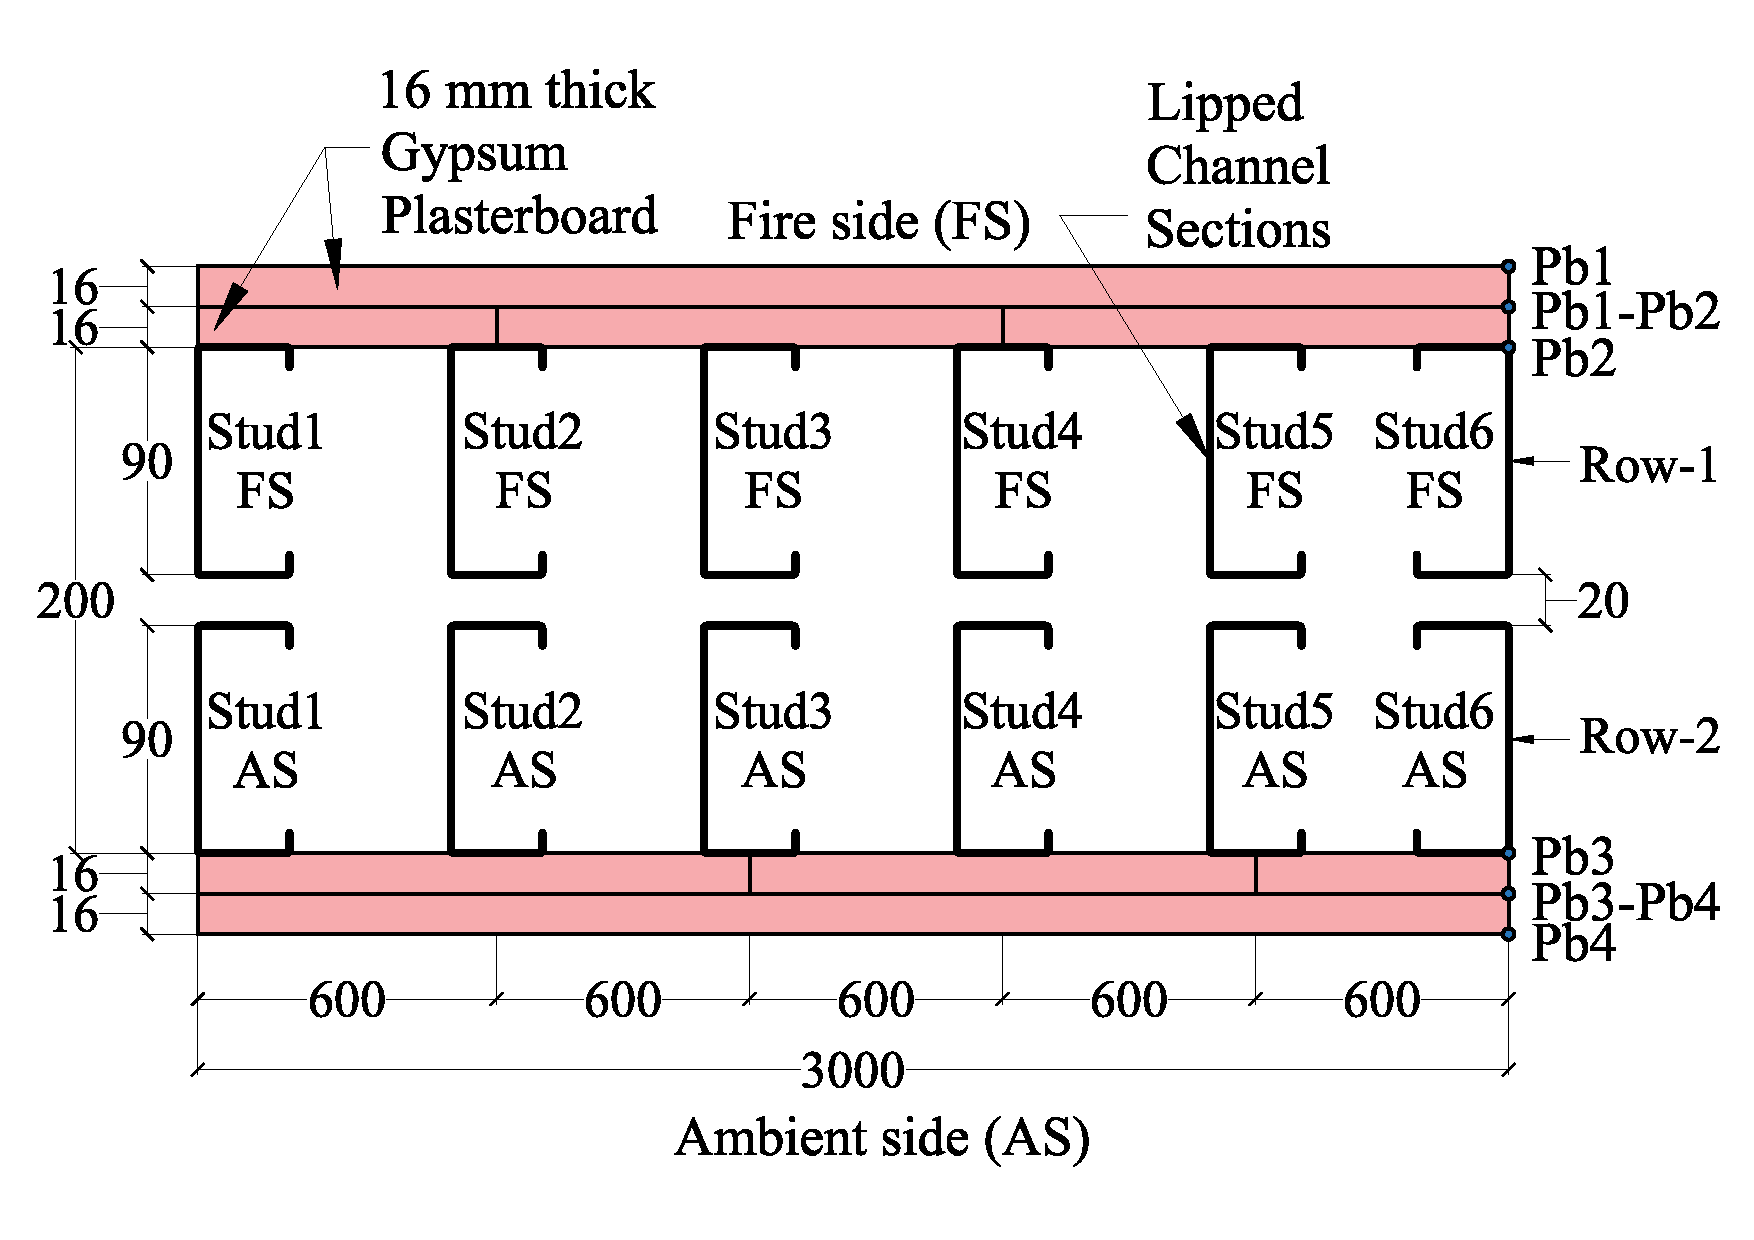
\includegraphics[width=8cm, height=5cm]{T1-plan} \\
			(a) \\
			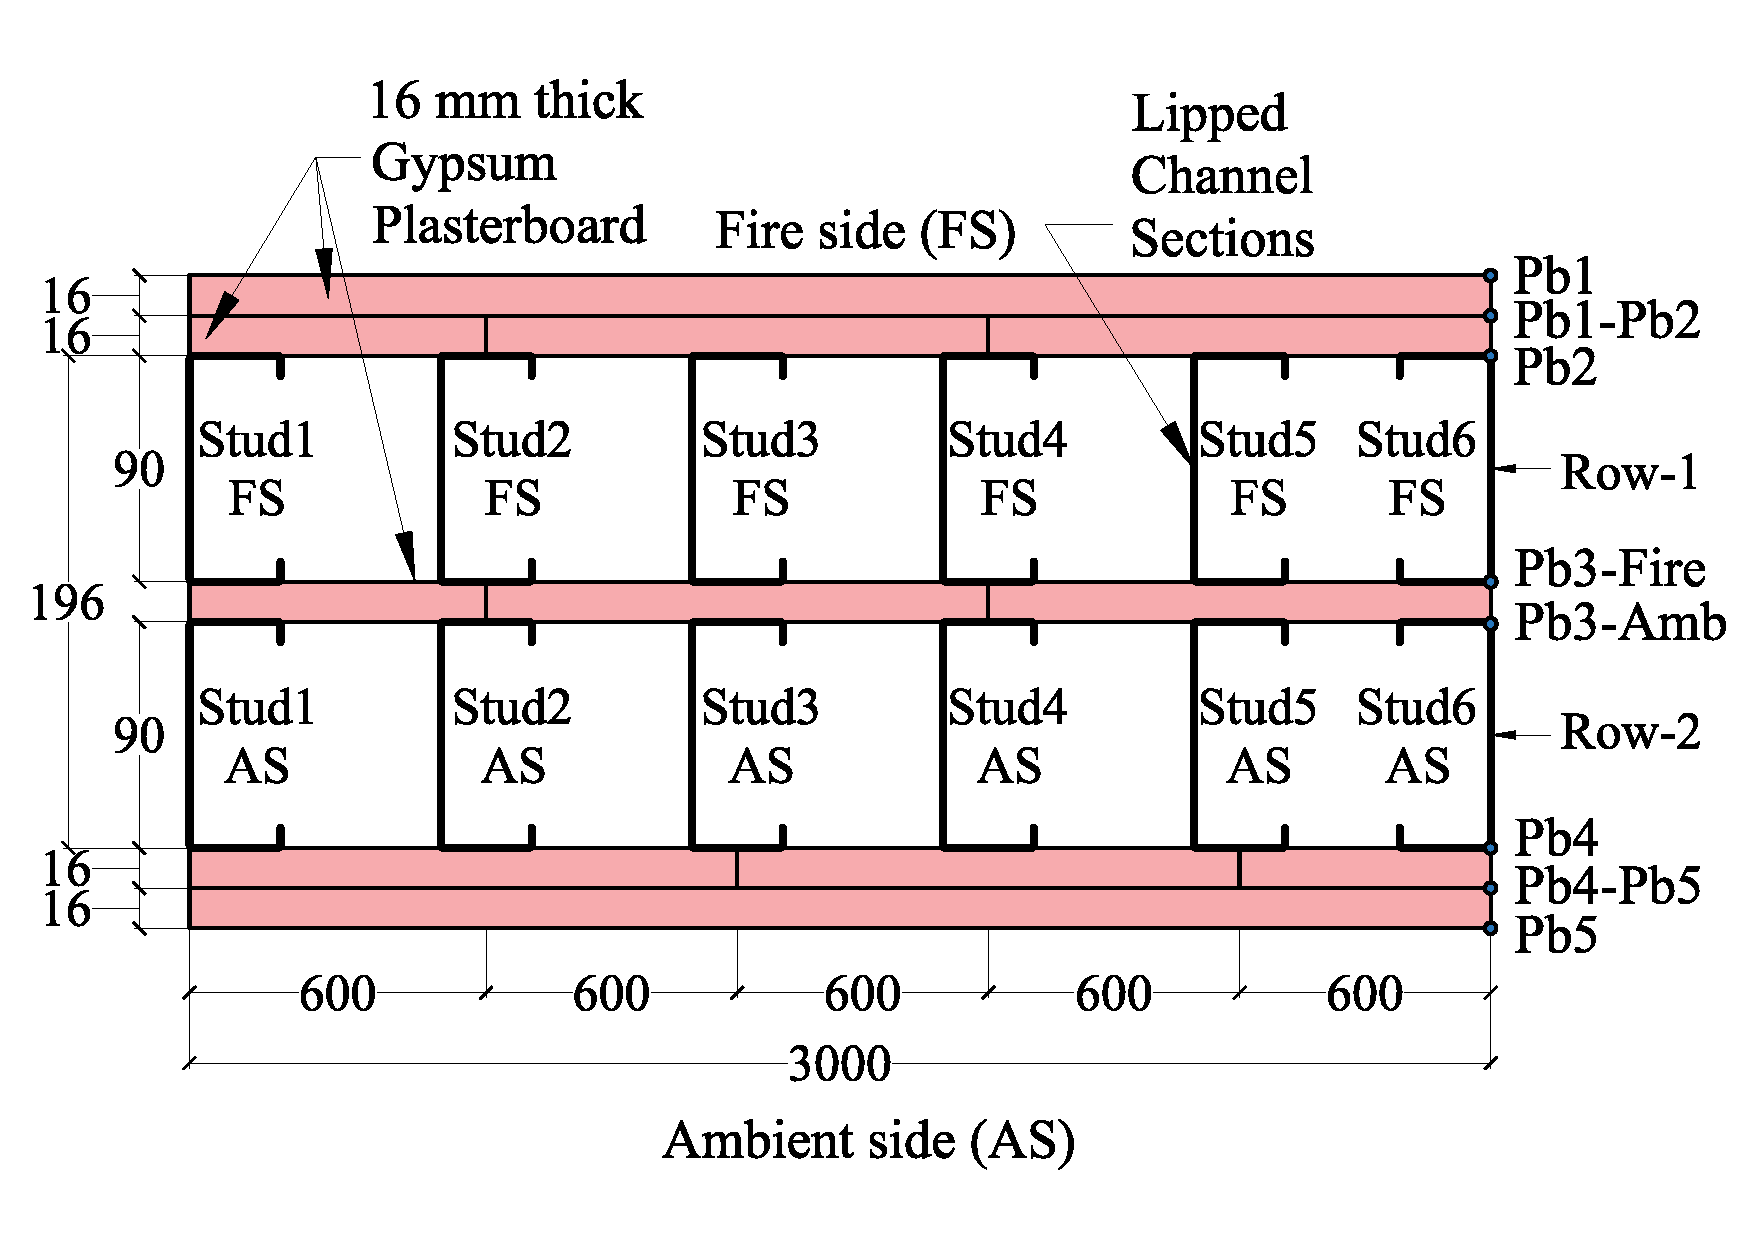
\includegraphics[width=8cm, height=5cm]{T8-plan} \\ 
			(b)  \\ 
			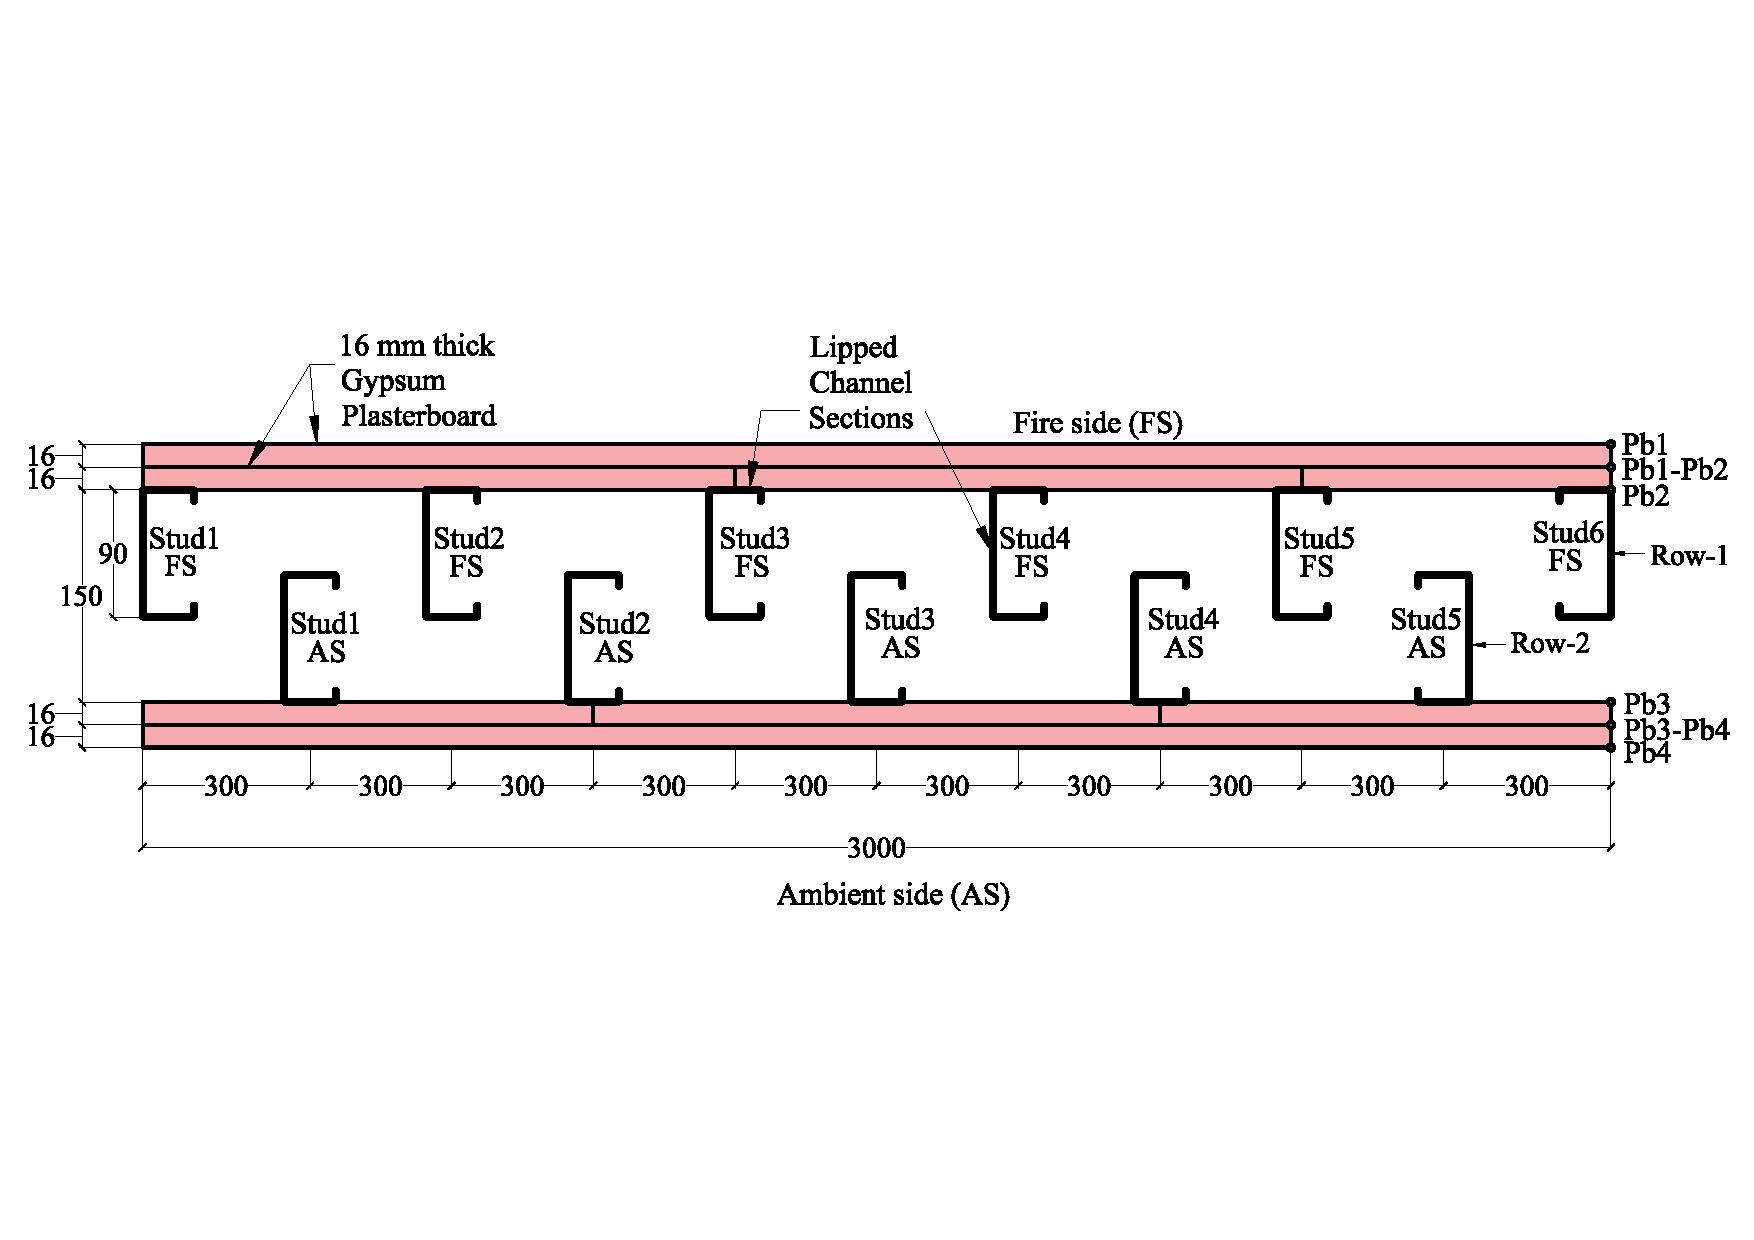
\includegraphics[scale=0.45]{T9-plan} \\ 
			(c)  \\ 
		\end{tabular} 
		\caption{Typical complex LSF wall configuration (a) Double stud (b) Shaftliner (c) Staggered stud }
		\label{fig:typical-complex}
\end{figure}

The construction of double stud LSF walls is also different from that of single stud walls. The double stud walls generally consist of a small air gap as shown in \Cref{fig:typical-complex}~(a) or may contain a shaft liner or a plasterboard layer between the stud arrangement as shown in \Cref{fig:typical-complex}~(b). These arrangements are present to split the cavity into two or more to yield a better fire and acoustic performance. The presence of two rows of studs in different arrangements within the LSF wall will increase the load carrying capacity of the wall system and its fire performance. This will be beneficial in mid-rise buildings as the loads on the walls will be higher when compared to low rise buildings.

\section{Research Problem}

Increasing the Fire Resistance Level (FRL) of LSF wall is the need of the day. Researchers implement their ideas to ultimately increase the FRL of wall systems and make it structurally stable so that in the event of fire outbreak loss of life due to structural failure can be nullified. Past research studies focused only on varying the plasterboards by changing the type of boards, increasing the number of plasterboard layers in the wall, changing the type of stud section, improving the thermal performance of plasterboard using an external insulation layer etc. to achieve higher FRL. Effects of the arrangement of studs inside the wall via more complex wall systems was not the primary focus in many research studies. Earlier investigations focused on walls with less than 3 m height, which are primarily used in residential buildings. In residential buildings, the acoustic insulation is not a major concern as the intensity of sound for transmission through the wall is minimum. But in movie theatres, studios and in wall partitions between houses in an apartment, acoustic insulation is very important and the wall height can exceed 3 m. Especially in situations where the wall height exceeds 3 m, single stud arrangement cannot be used as the cold-formed steel sections are slender in nature. In these situations, complex wall systems with double rows of studs with or without a middle layer of plasterboard or shaftliner can be used. They can also be used as staggered stud wall systems (\Cref{fig:typical-complex}). Similarly, with the focus on developing mid-rise building systems using cold-formed steel members, LSF wall systems with complex wall systems are needed in the lower storeys for higher load bearing purposes. In mid-rise buildings, the axial compression load acting on the bottom stories will be higher when compared with the top levels. Fire resistance and structural adequacy of building components in mid-rise buildings are utmost importance to prevent a structural collapse during fire outbreak. However, past research has addressed only the thermal and structural behaviour of LSF wall systems with single row of studs. This research will therefore focus on the complex LSF wall systems with double and staggered stud LSF wall systems. 

Another important research problem is the lack of a robust numerical model and analysis technique for LSF walls exposed to fire conditions. Many parameters such as free water evaporation from the plasterboard, effects of cavity radiation due to heat transfer from one face of the wall to another, pressure build-up within the cavity due to heat transfer and air movement within the cavity through natural convection were not considered in the past numerical modelling studies to reduce the complexity of numerical analysis. 

Fire tests of load bearing and non-load bearing walls are an effective means to investigate the thermal and structural performance of complex LSF wall systems. But when the cost and time consumed in these tests are taken into consideration, it becomes uneconomical and practically impossible to study many iterations of wall systems within a short span of time. With the advancement of high-performance computing in recent times, it becomes beneficial for the researchers to study the thermal and structural behaviour of LSF walls with ease. Finite element analysis (FEA) is considered as the key to many multi-physics problems. Research on the thermal and structural performance of LSF wall systems is carried out using FEA software such as ABAQUS, ANSYS etc. Most common heat transfer problems such as combustion inside an engine is modelled and analysed by Computational Fluid Dynamics (CFD) technique as heat transfer happens in 3-dimensionsional space. Past research has focused on modelling the design or real fire as 1-dimensional entity only. Therefore, attempts should be made to use CFD models to investigate the thermal behaviour of complex LSF wall systems by considering the fire loads in 3-dimensional space.

\section{Research Aim}

The aim of this research is to investigate the thermal and structural performance of selected complex double and staggered stud LSF wall systems using full scale standard fire tests and advanced numerical modelling. The key tasks of this research to achieve this aim are as follows. 
\begin{itemize}
	\item Undertake a detailed review of complex LSF wall systems and their fire performance, and thermal and mechanical properties of wall components and, establish their appropriateness.
	\item Conduct a series of full scale standard fire tests of double and staggered stud wall systems to investigate their thermal and structural performance in fire. 
	\item Compare the full-scale fire test results with the available fire test results of conventional single stud wall systems to evaluate the effects of complex stud arrangements on structural and thermal performance.  
	\item Develop advanced finite element models to simulate the thermal and structural performance of double and staggered stud wall systems exposed to fire conditions and validate them using full scale fire test results.
	\item Improve the fundamental understanding of the thermal and structural performance of double and staggered stud wall systems through the use of validated finite element models in investigating the LSF wall behaviour and failure modes of studs in detail.
	\item Undertake a detailed parametric study of double and staggered stud wall systems with different structural and thermal parameters of LSF wall components. 
	\item Investigate the suitability of existing fire design rules in the Australian and European fire design standards for complex LSF wall systems and if needed, develop improved fire design rules and simple design methods to predict the fire resistance levels and axial compression capacities of cold-formed steel studs in complex LSF wall systems exposed to fire.
\end{itemize}

\section{Outline of Thesis}

Based on the research aim and the specific tasks as listed above, this research was conducted in a sequential manner and a brief outline of the contents included within the chapters are presented next.

\textbf{\Cref{ch:Literature}} details the extensive literature review conducted on LSF walls. Topics include the ambient and fire performance of simple and complex LSF wall assemblies. This covers the experimental and numerical investigations on LSF walls. Initial investigations were carried out by sampling the real-time problems faced by the LSF wall industry with respect to complex wall systems (double and staggered stud walls). Literatures were collected and reviewed to identify the problems to be taken up for the current research. Ground surveys by contacting industry experts to know about the current practice in the complex LSF wall arrangements such as double and staggered stud walls were carried out to determine the best possible complex LSF wall configurations to be investigated in the current study. Finally, a summary of the reviewed literature was made and the possible techniques to address the research aim are proposed.

\textbf{\Cref{ch:Ambient}} presents the ambient temperature capacity test results conducted on selected complex LSF walls based on the detailed literature review. Test results include the axial compression capacity, axial displacement and lateral deflection curves. The buckling behaviour of studs in double and staggered LSF wall configurations under axial compression is also discussed in detail. Numerical investigations through finite element analyses conducted on double and staggered LSF wall configurations to predict the ambient axial compression capacity are also discussed. 

\textbf{\Cref{ch:Fire}} reports the findings of one small scale fire test and 10 full-scale fire tests conducted on double and staggered LSF wall systems. Illustrations are made for the tested complex LSF wall configurations and fire test results in the form of time-temperature curves are presented in detail. Increase in the FRL of the complex LSF walls was noticeable in comparison with similar single stud LSF wall assemblies. The detrimental effect of cavity insulation in complex LSF walls was also investigated. Detailed comparison of the fire test results are made against full-scale fire test results of single stud LSF walls and the unique heat transfer mechanism in complex LSF walls are summarised. 

\textbf{\Cref{ch:FE-Thermal}} presents the developed FE thermal models to predict the thermal performance of complex LSF wall systems. Firstly, three different software packages were used to develop thermal models and a detail comparison was made amongst them to find the most appropriate software package to use for developing the thermal models. A detailed comparison was made considering the advantages and shortcoming in the thermal model results and the numerical model results were validated against the conducted small-scale and full-scale experimental results to establish the suitability of the model. Based on the developed model, a detailed parametric study was conducted on complex LSF wall configurations to predict the fire performance and the corresponding results were also discussed in detail.

\textbf{\Cref{ch:FE-Structural}} details the FRL predictions from structural model which was developed alongside the thermal models to predict the structural behaviour of the studs in fire. The structural model inputs were extracted from the fire test results from \Cref{ch:Fire,ch:FE-Thermal} and the FRL predictions were made. Non-cavity insulated LSF walls were found to result in better FRL in comparison with cavity insulated LSF walls. The FRL predictions were made based on different load ratios based on the axial compression capacity determined in \Cref{ch:Ambient}.

\textbf{\Cref{ch:FE-Parametric}} presents the parametric analysis results conducted from FE thermal and structural models. The parameters for the stud includes different wall configurations and stud thicknesses. FRLs of the selected wall configurations are presented in table and the closest FRL in min corresponding to the BCC is also provided. 

% \textbf{\Cref{ch:Design}} covers the DSM based failure time predictions for complex LSF wall configurations under different load ratios. The suitability of the existing equations used for single stud LSF walls in predicting the failure times for complex LSF walls was investigated and summarised. The suitability of the existing design equations in comparison with the numerical models is also discussed.

\textbf{\Cref{ch:Conclusions}} provides a summary of the findings from this research study. Conclusions are drawn from the experimental and numerical investigations and suitable recommendations are also proposed for future work in relation to the fire performance of complex LSF walls.

  

\chapter{Literature Review}
\label{ch:Literature}       
\section{Background}
The importance of fire protection in buildings has become an important concern in recent times. Fire outbreak in buildings has led to significant loss of life and property in many instances. Some major fire accidents in recent times leading to considerable loss of life and severe damage to the property are shown in \Cref{fig:Major fire accidents}. 
\begin{figure}[htbp]
	\centering
		\begin{tabular}{ccc}
			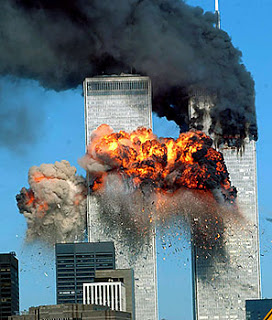
\includegraphics[width=4cm,height=5.5cm]{wtcfire} & 
			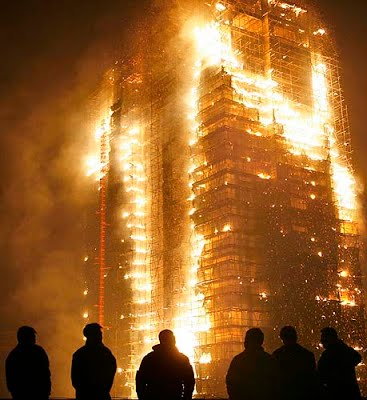
\includegraphics[width=4cm,height=5.5cm]{londonfire} &
			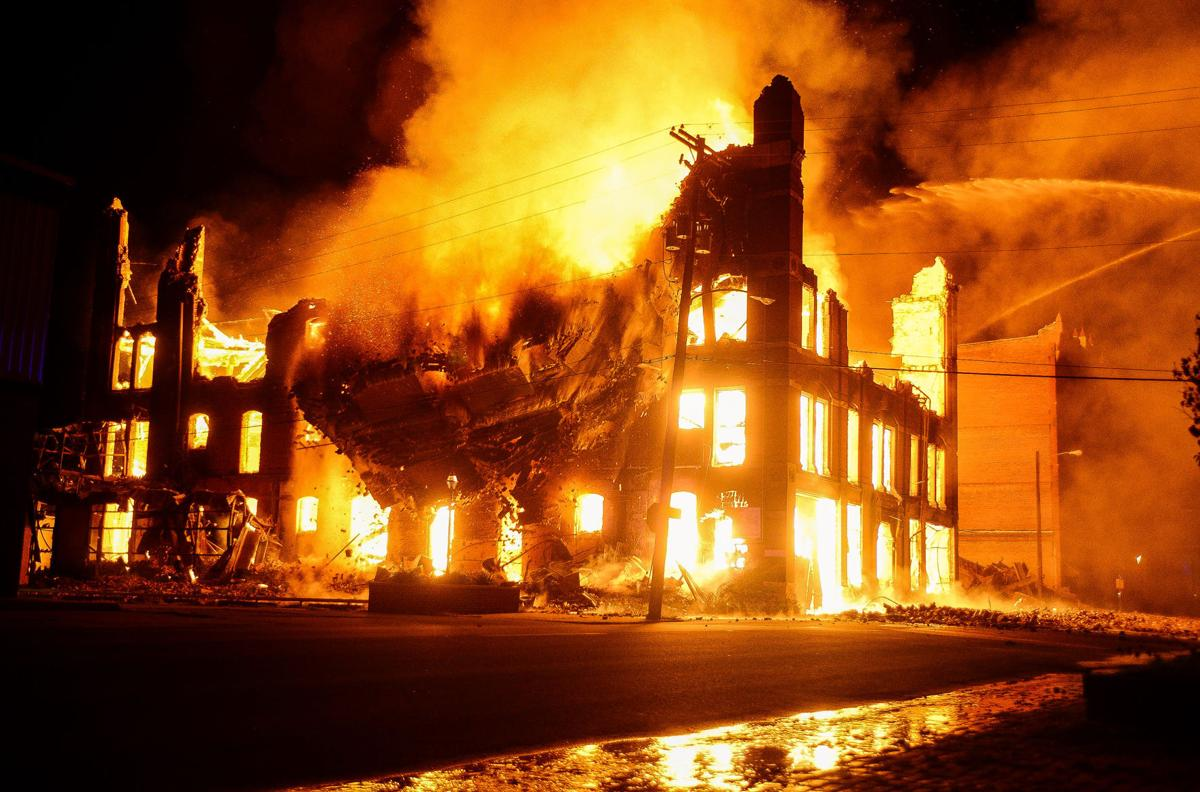
\includegraphics[width=4cm,height=3.5cm]{empirefire} \\ 
			(a) & (b) & (c) \\ 
		\end{tabular} 

	\begin{scriptsize}
	Images extracted from \url{https://images.google.com.au/}
	\end{scriptsize}
	
		\caption{Major fire accidents in recent times}
		\label{fig:Major fire accidents}
\end{figure}

This has led the researchers to concentrate on the fire safety of buildings. Most common form of building constructions include materials which are more susceptible to fire exposure. For instance, the major components of a residential building include concrete, hot-rolled steel and wood. The fire performance of a building is greatly dependent upon the fire performance of these individual materials. Therefore, researchers focus on these materials and are keen to improve the performance of these materials under fire exposure. During a fire incident, the structural elements of a building are subjected to additional fire loads apart from the existing dead and imposed loads. This results in premature failure of the structural members if they are not properly designed to take the fire loads apart from the structural loads. As this research is focused on the complex LSF walls used in buildings, past literatures with respect to this are summarised in detail.

\section{Experimental and Numerical Investigations of LSF Walls}

The LSF walls used in buildings are load bearing and non-load bearing. The non-load bearing walls are generally used in partition separations in a RCC framed buildings whereas the load bearing walls are generally found in day to day low rise to mid-rise residential buildings. This section gives a detailed insight of the experimental and numerical investigations carried out in both load bearing and non-load bearing LSF walls in the past.

\citet{Son} experimentally investigated the fire performance of partition walls under load bearing conditions as per ASTM E119-71 standards using two fire tests. The test wall dimensions were 8 foot high and 16 foot long. Lipped channel section was used as studs in the former while the later used tubular sections as studs in the wall assembly. 18 ga (1.02 mm) thick steel studs where used. Both the test specimen consisted of two plasterboard sheathed frames separated by 1/2 inch cavity. The plasterboards were 5/8 inches thick for both the fire tests, but the thermomechanical properties of the same was unavailable. Single layer of Type X gypsum plasterboard was used on both the test specimen. 3 1/2 inch thick glass wool compressed to 3 inch was used as the insulation. However the sound insulation values and the material properties were not provided in detail. During fire test, the phenomenon of thermal bowing was noticed and reported. Inward thermal bowing was significant where, the test specimen bowed towards the furnace. The first test wall with lipped channel section survived for 75 min after which flames where visible on the unexposed side. The second test wall with tubular studs survived for 97 min after which visible smoke were seen through cracks on the unexposed side of the test wall. Time-temperature curves were plotted for the plasterboards, but the individual stud time-temperature curves were not available. It was suggested that the usage of two layers of Type X gypsum plasterboard will increase the fire rating level (FRL).   

The history of fire tests dates back over a century. \citet{Babrauskas1978} summarised the fire tests conducted from 1880 to 1918 and listed the key features in conducting fire tests on walls. The report was summarised into two parts. The first part reported about the history in forming the fire testing standards, while the second part described about various fire tests carried on different building elements across the globe. It was mentioned that ASTM E119 earlier C19 was the first standard issued on the fire testing of building elements. This report included the major fire tests from the year 1880 and tried to summarise all the fire test reports available in English during that time. However, test reports in other languages were ignored due to the difficulties in interpretation. The need for fire proofing on steel,concrete and timber elements back then was debatable and the necessity for the same was explained. The first report explained in detail about the very first fire test on walls and the difficulties in measuring the temperatures during the fire test. Fire testing on columns were also reported in detail. Details about the fire tests on walls were summarised in second part of the report.  

It was reported that the first controlled fire test was carried out in Germany in 1891 on a small hut. This emphasised the importance for fire tests over a century ago. The test room was constructed using timber studs and had the dimensions of 2.01 m $\times$ 2.63 m $\times$ 2.63 m respectively. The author also described about the Vienna column test in 1893 and exclaimed that the test was not carried out as per required standards and should be ignored. From this report it is evident that until early 1900's the fire tests were carried out on whole compartment rather than individual building elements. All the fire tests were carried out in a gas-fired chamber, but the dimensions of the test specimens were not consistent. The usage of different organic building elements at different time period were also reported. From the year 1915 it was reported that the furnace dimensions were increased to 3.6 m $\times$ 4.5 m $\times$ 0.4 m. This was the new standard for testing the wall specimens in Underwriters Laboratory (UL) and thermocouples were used for temperature measurements instead of thermometers. Apart from the tests on walls, the report also elaborated the fire tests on other building components such as doors and openings. However, temperature distribution across the wall was not reported in detail. The establishment of the standard fire curve in the year 1917 and the inclusion of the same into the ASTM E119 standards was also described in detail. This also included various failure criteria for different building elements and their level of fire protection. Also, the validation checks conducted to verify the suitability of the standard fire curve was also discussed in detail.

\citet{Klippstein1978} used the fire test results conducted on LSF walls based on ASTM E119 to propose analytical methods to predict the structural failure time in gypsum plasterboard sheathed LSF walls. Initially, the author conducted tests to determine the mechanical properties of the steel sections used in the LSF wall. The test walls used for this study were 3.05 m $\times$ 3.05 m. Only the axial loads were considered in the fire design while the wind loads were neglected for the calculations. The phenomenon of plasterboards losing the effective lateral restraints on to the studs at elevated temperatures were discussed in detail. The concept of load sharing in LSF walls was also discussed whereby the load being shared to the stronger studs (less temperatures) during full-scale fire test. Failure of the stud was assumed to happen by weaker axis only in formulating the design equations. The concept of load ratio (LR) $P_T/P$ was used, where $P_T$ is the calculated failure load at elevated temperature $T$ while P is the failure load at ambient temperature. The failure load was determined theoretically using the following equation.
\begin{equation}
	P = \dfrac{23}{12} F_{al}A
\end{equation}
Elastic buckling was the governing failure mode in studs more than 4.5 m height assuming the end conditions to be pinned. As the studs in LSF walls are generally 3 m tall inelastic buckling was the critical failure mode. The equation to predict the inelastic buckling load was proposed as below. 
\begin{equation}\label{eq:inelastic}
	F_{al} = \dfrac{12}{23} QF_y-\dfrac{3}{23}\dfrac{(QF_y)^2}{\pi^2E}\left(\dfrac{KL}{r}\right)^2 	
\end{equation}
Where
\begin{description}[itemsep=0pt,parsep=0pt]
	\item $Q$ = strength reduction factor at room temperature
	\item $F_y$ = actual yield strength at room temperature
	\item $E$ = modulus of elasticity at room temperature
	\item $K$ = effective length factor of the stud
	\item $L$ = length of the stud
	\item $r$ = radius of gyration about major axis.
\end{description}	
Based on the above equation \cref{eq:inelastic} the failure load at room temperature was determined using the equation below.
\begin{equation}
	P = \left[QF_y - \dfrac{1}{E}(\dfrac{QF_yL}{2\pi r})^2\right]A
\end{equation}
During fire test, the studs laterally deflect causing bending stresses and these effects have to be included in calculating the $P_T$. Therefore, the interaction equation for combined axial and bending action available in the AISI manual was used and is given below.
\begin{equation}
	\dfrac{f_a}{F_{alT}} + \dfrac{C_{mx}}{\left(1-\dfrac{f_a}{F'_e}\dfrac{f_b}{F_{blT}}\right)} < 1.0
\end{equation} 
Where
\begin{description}[itemsep=0pt,parsep=0pt]
	\item $f_a$ = compressive stress due to axial load
	\item $F_{alT}$ = allowable stress for axial load at failure temperature
	\item $\dfrac{C_{mx}}{\left(1-\dfrac{f_a}{F'_e}\dfrac{f_b}{F_{blT}}\right)}$ = modification factor for bending stresses
	\item $f_b$ = bending stress at mid-height
	\item $F_{blT}$ = allowable bending stress at failure temperature
	\item $F_{yT}$ = allowable strength at failure temperature
	\item $Q_T$ = column-strength reduction factor at failure temperature
	\item $E_T$ = modulus of elasticity at failure temperature
\end{description}
Based on the above mentioned equations the load ratio (LR) was computed by the following equation.
\begin{equation}
	LR = \dfrac{1}{\left(\dfrac{1}{F_{alT}}+\dfrac{23 A \delta _T}{128_xF_{yT}}\right)F_{al}}
\end{equation}
To determine the capacity reduction in the members, material properties at elevated temperatures were determined by the authors and were used in the above mentioned equations. It was found that at elevated temperatures, the elastic modulus of sheet steel decreased rapidly in comparison with that of plate steel. Stub column tests were also conducted to determine the column strength reduction factor at elevated temperatures. The proposed equations resulted in conservative results in comparison with the experiments.

\citet{Gerlich1996} investigated the design of LSF walls under standard ISO 834 fire curve and some real fire curves. This research proposed methods for calculating the reduction in strength of steel studs in the LSF wall at elevated temperature and methods for predicting the deflections in the cold-formed steel studs which occurs as a resultant of elevated temperature gradients and P-$\Delta$ effects. Three design codes AS 1538, BS 5950 and AISI design manuals were compared for the limit state design of cold-formed steel sections at room temperature. It was found that the AISI design manual gave accurate capacity predictions. The experimental structural test was initially carried out for 3m length columns under axial loads and bending to verify the AISI design methodology at ambient conditions. An equation for specific heat (k) until 900\degree C of fire exposure was also developed.

\begin{equation}
k = -0.022T + 48, for 0 < T < 900\degree C
\end{equation}

It was concluded that with the help of experimental and analytical studies, the P-$\Delta$ effect at elevated temperatures can be predicted with good accuracy. Buckling of the compression flange of cold-formed steel stud on the ambient side was the main cause of structural failure at elevated temperatures.

\citet{Alfawakhiri1999} reviewed the fire resistance of the load bearing steel stud walls protected with gypsum board. It was suggested that there were robust experimental methods to test the thermal performance of LSF walls, but there was a gap in the numerical analyses and the design procedures or the LSF walls. This review also mentioned about the low data sets available because of fire test which may cause inaccuracy in the design procedure. The importance of using insulation such as mineral wool, glass fibre, cavity insulation etc, within the wall was highlighted. The thermal conductivity of various gypsum boards were discussed and a relationship was established between thermal conductivity and temperature. Likewise, the relationship between specific heat and temperature was also developed. The variation in the modulation of elasticity of the cold formed steel sections with respect to temperature was also reviewed. It was concluded that factors such as specific heat, thermal conductivity, modulus of elasticity of studs with variation in temperature will have a significant effect on the fire performance of the steel studs.   

\citet{Sultan2000a} summarised the performance based parameters to be considered while designing LSF walls. A total 17 previously conducted full-scale fire tests were considered as reference for this study to arrive at different parameters that were important in designing LSF walls under fire. All the considered wall specimens were 3 m high and 3.7 m wide. Both steel and wood stud assemblies were considered for this study. However, the wall specimens were constructed using gypsum plasterboard only. Also, this study comprised of load bearing tests for wood studs only. All the steel stud assemblies considered were non-load bearing. The reference fire tests were carried out in accordance with CAN/ULC-S101-M89 (\citeyear{ULC1989}). It was found that the presence of cavity insulation will result in rapid increase of the plasterboard temperatures in comparison with uninsulated wall assemblies. The average temperature on the unexposed side of the test wall was lower in specimens with rock fibre insulation in comparison with non-insulated assemblies. Presence of cavity insulation in non-load bearing LSF wall assemblies resulted in increased FRL. However, the effect of insulation in loadbearing LSF walls were not discussed in detail. It was also reported that, the type of insulation did not significantly affect the FRL, provided the insulation had a perfect fit between the studs resulting in no loose gaps.

Another important finding was that the presence of resilient channels and proper positioning of the same, significantly increased the FRL in non-load bearing LSF wall assemblies. However, the effective restraints provided by the resilient channels along with the plasterboards were not reported in detail, as all the tests in LSF walls were carried out under non-load bearing conditions. The presence of second layer of plasterboard with staggered joint arrangement significantly increased the FRL in comparison with single plasterboard layer. It was reported that under non-load bearing conditions, the type of stud such as wood or steel did not affect the FRL.  

\citet{Collier2002} reviewed the BRANZ method of height extrapolation to study the resistance of non-load bearing steel framed walls under fire. Floating stud system was chosen for the study. The wall specimen chosen was set at 4 m $\times$ 4 m panel in comparison to the conventional 3 m $\times$ 3 m panel. The flexural rigidity of the horizontal joints tend to fail prematurely in comparison with vertical joints when exposed to fire. This premature failure can expose the flanges of stud directly to the path of fire propagation. This research also compared the test results between wall panels with and without the vertical lining joints.

\citet{Feng2003c} studied the thermal performance of cold-formed thin-walled steel panel systems under fire using small-scale fire tests 1.5 $\times$ 1.5 $\times$ 1.5 m. The performance of gypsum board under severe fire conditions was the principal focus of this research. Focus was given in developing a finite element model to predict the thermal performance of gypsum boards and steel studs. Lipped channels were considered in this study. Time-temperature curves were plotted for panels tested with different layers of gypsum board and insulation under fire. Combination of studs with service holes in the panel were also considered in the fire test. ABAQUS finite element analyses were conducted for the numerical validation of the fire tests. Material properties of the gypsum board, steel studs and insulation in BS EN 1993-1-3 (2006) Part 1.2 were used.

The test results were compared with the FEA results and several conclusions were made as follows. The free water content present in the gypsum boards was not considered in the numerical analysis. Hence the results from the ABAQUS  were reasonable, but were not accurate in accordance with the experimental results. Different layers of gypsum boards along with insulation on the fire side were used both in experiments and analyses and it was found that the steel stud temperature had a high influence on the usage of insulation and not the number of layers of gypsum board on the exposed side. It was concluded that increasing the number of gypsum boards increased the FRL. The failure of gypsum boards on the exposed face, did not promote fire spread to the unexposed face due to the presence of insulation. Isowool and Rockwool insulations were used and the results were compared with a non-insulated wall panel. It was found that, the presence of insulation on the fire exposed side of the wall resulted in higher stud temperature. The thermal performance of the wall might get affected if the insulation is provided on the unexposed face of the wall to reduce cold bridging in warm construction. The shape of the thin-walled cold-formed steel cross section had the least effect on the thermal performance, whereas in the case of a cassette section the thermal performance was affected by its layout.  

Based on the fire test results \citet{Feng2003d} investigated the structural behaviour of LSF wall panels. Numerical analysis and design calculation were carried out based on 52 channel sections with FE package ABAQUS. Modified design equations for channel sections were proposed to include the effects of distortional buckling failure and change in strength and stiffness of steel at elevated temperatures based on BS5950 Part 5 and Eurocode 3 Part 1.3. It is to be noted that the design of the channel sections included the service holes present in the steel studs. The ultimate strength of the studs with service holes were determined by AISI(1996) code of practice. The geometric non-linearities, imperfections and stress-strain relationships at elevated temperatures were also considered for the design and were based on Eurocode 3 Part 1.2 or \citet{Outinen1997}. The equation for calculating the effective width of a flange for distortional buckling was modified as follows.

\begin{equation}
\dfrac{b_{eff,de}}{b}= 1 for \lambda \leq 0.673
\end{equation}

\begin{equation}
\dfrac{b_{eff,de}}{b}= \sqrt{\dfrac{\sigma_{de}}{f_y}}\bigg(1-0.22\sqrt{\dfrac{\sigma_{de}}{f_y}}\bigg) for \lambda \geq 0.673
\end{equation}

To calculate the effective width of the web, the considerations were taken from AISI standards. The web is considered as a solid web if $a/h$ is $< 0.38$ and the web is considered to consist of two unstiffened elements if the $a/h$ is $> 0.38$ as pr AISI S100-12 (2012) specification as shown in Figure.\ref{fig:feng_buckling}. Based on the design modifications and numerical analysis, it was concluded that the design modifications and numerical analysis, it was concluded that the design formulations used for ambient capacity calculation can be extended and used for elevated temperatures as well. This is achieved, when the reduced yield strength derived from 0.2\% proof stress and the reduced elastic modulus are used. 

\begin{figure}[htbp]
	\centering
		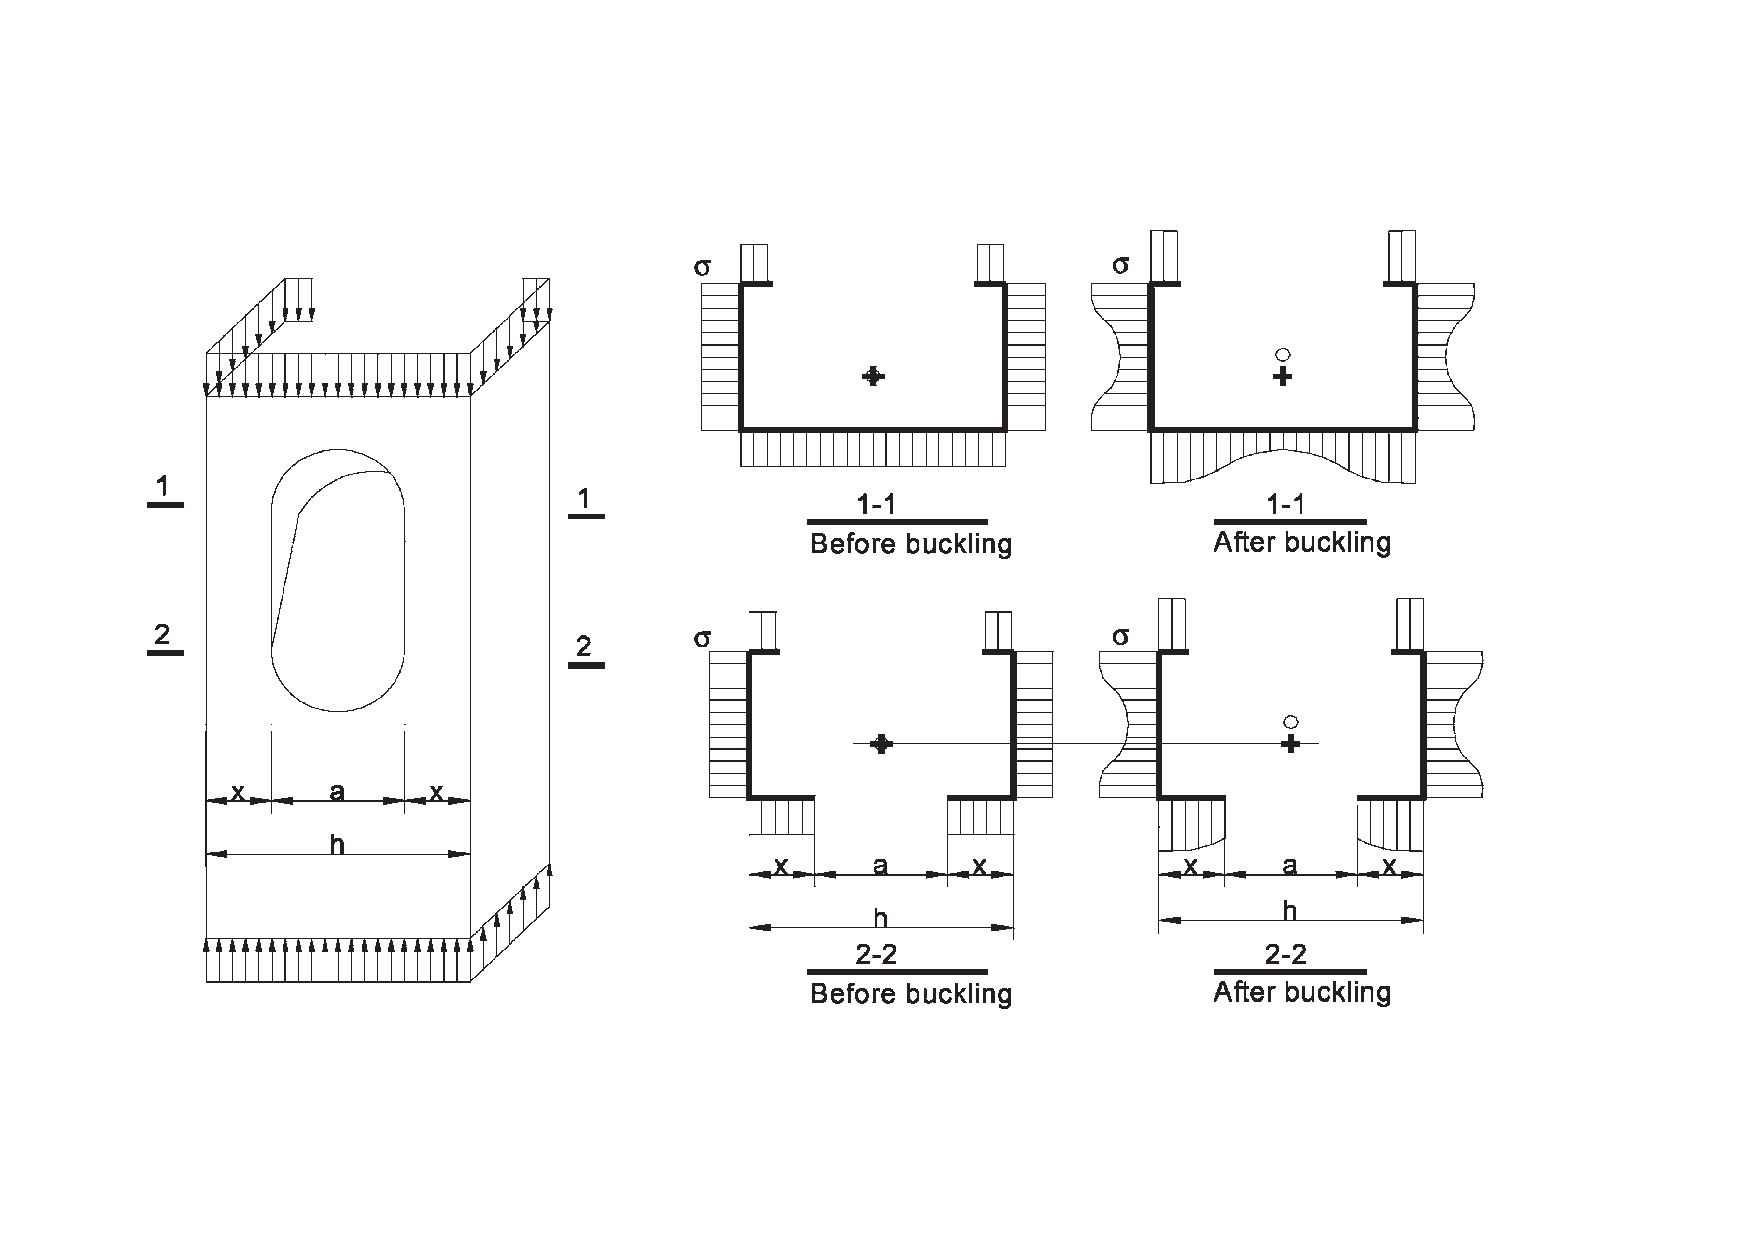
\includegraphics[width=10cm,height=6cm]{feng_buckling}		
		\caption{Lipped Channel with Service Holes used by \citet{Feng2003}}
		\label{fig:feng_buckling}
\end{figure}

The effect of distortional buckling can be included for design calculations based on \citet{Young1992}. Service holes can be considered in the design, based on AISI specifications. ABAQUS can be used to stimulate the behaviour of cold-formed steel sections at elevated temperatures, provided proper material properties and boundary conditions are used.

\citet{Feng2003} extended the study to investigate the axial strength of CFS channels under non-uniform elevated temperatures due to fire. Two methods were adopted for the design process. First the EN1993-1-3 ambient temperature design equation was modified and the second using the limiting temperature method. The design equations for the cold-formed steel columns under combined axial load and bending moments were based on the following equations from Eurocode 3 Part 1.2.

\begin{equation}
\dfrac{N_{sd}}{\chi_{min}f_{yb}A_{eff}}+\dfrac{k_y(M_{y,sd}+\Delta M_{y,sd})}{f_{yb}W_{eff,y,com}}+\dfrac{k_y(M_{z,sd}+\Delta M_{z,sd})}{f_{yb}W_{eff,z,com}} \leq 1
\end{equation}

\begin{equation}
\dfrac{N_{sd}}{\chi_{lat}f_{yb}A_{eff}}+\dfrac{k_y(M_{y,sd}+\Delta M_{y,sd})}{f_{yb}W_{eff,y,com}}+\dfrac{k_y(M_{z,sd}+\Delta M_{z,sd})}{f_{yb}W_{eff,z,com}} \leq 1
\end{equation}

Later the results from the modified design equations from the EN1993-1-3 were compared with ABAQUS simulation results. 100 x 54 x 15 x 1.2 mm lipped channel sections were used in the study. The FE modelling in ABAQUS was carried out with S4R shell elements. Appropriate restraints were applied to the studs to replicate the full-scale fire test. Steady state method of heat transfer analysis was carried out. Sequential uncoupled FE analysis was carried out in ABAQUS. It was found that the failure temperature of the stud sections was similar in the experimental and numerical study irrespective of the number of plasterboard layers. The presence of more than single layer of plasterboard ultimately delayed the temperature of the studs only. 

\citet{Sakumoto2003} conducted experimental studies on the fire resistance of walls and floors using various light gauge steel shapes. Partition walls and exterior walls were the main aim of the study. The wall specimens consisted of studs ranging from 0.5 to 1.6 mm and 12.5 mm thick plasterboards. The test specimens were 1820 mm wide and 2700 mm tall. Unlike other fire tests, the partition walls consisted of two rows of studs separated by 9 mm plywood between. The studs were lipped channel sections with different depths ranging from 89 mm to 235 mm and were spaced at 500 mm centres. Two layers of non-fire rated plasterboards were present on either side of the wall and an axial load of 34 kN was applied to some specimens. Glass wool insulation was present on both cavities in the partition wall for the specimen which resulted in highest FRL. The fire tests were carried out based on ISO 834 standard fire curve. The fire tests for the partition walls were carried out by varying the studs and the configuration with plywood between the rows of stud resulted in the highest with 67 minutes of FRL. Likewise different floor-ceiling configurations were also tested for FRL. The specimens used for the floor-ceiling tests were bigger than that of the wall tests. The specimens were 2950 mm wide and 4260 mm long. FRLs of more than 60 minutes were achieved for some configurations. It was concluded that the gypsum board fall-off was an important criterion in determining the FRL. The plasterboard fall-off can be reduced by increasing the number of plasterboard layers. The collapse temperature, time and sequence of failure of the structural members in the LSF wall were also detailed. Most of the tests conducted on wall panels had single layer plasterboards and the FRL was about 45 minutes. In the case of wall panels with plywood the FRL was just above 60 minutes. 

\citet{Feng2005} investigated the cold-formed, thin-walled steel panels with service holes in fire. The holes were provided in the channel sections, one near the top and one near the bottom. Full-scale tests were carried out at different load ratios of 0.2, 0.4 and 0.7 times the axial load carrying capacity of the channels at ambient temperatures. The main observation in the failure of the steel studs was that the studs failed by local buckling near the service holes at ambient temperature. Flexural-torsional buckling along the major axis with lateral deflection caused by thermal bowing due to the temperature gradients was also observed in this study. Increase in the stud temperature was noticed during some tests due to the complete burning of the insulation layer provided in the panel. Detachments of the fasteners along the unexposed side of the panels were noticed during the test. 

\citet{Manzello2005} studied the performance of partition assemblies under real fire. This research was different from the existing approach as their fire test was performed in real-scale compartment instead of a conventional furnace setup. This test was carried out for non-load bearing conditions. A compartment as shown in \Cref{fig:manzello_compartment} was constructed and the fire curve based on ASTM E119 was simulated within the compartment and the thermal performance of the partition walls was investigated.

\begin{figure}[htbp]
	\centering
		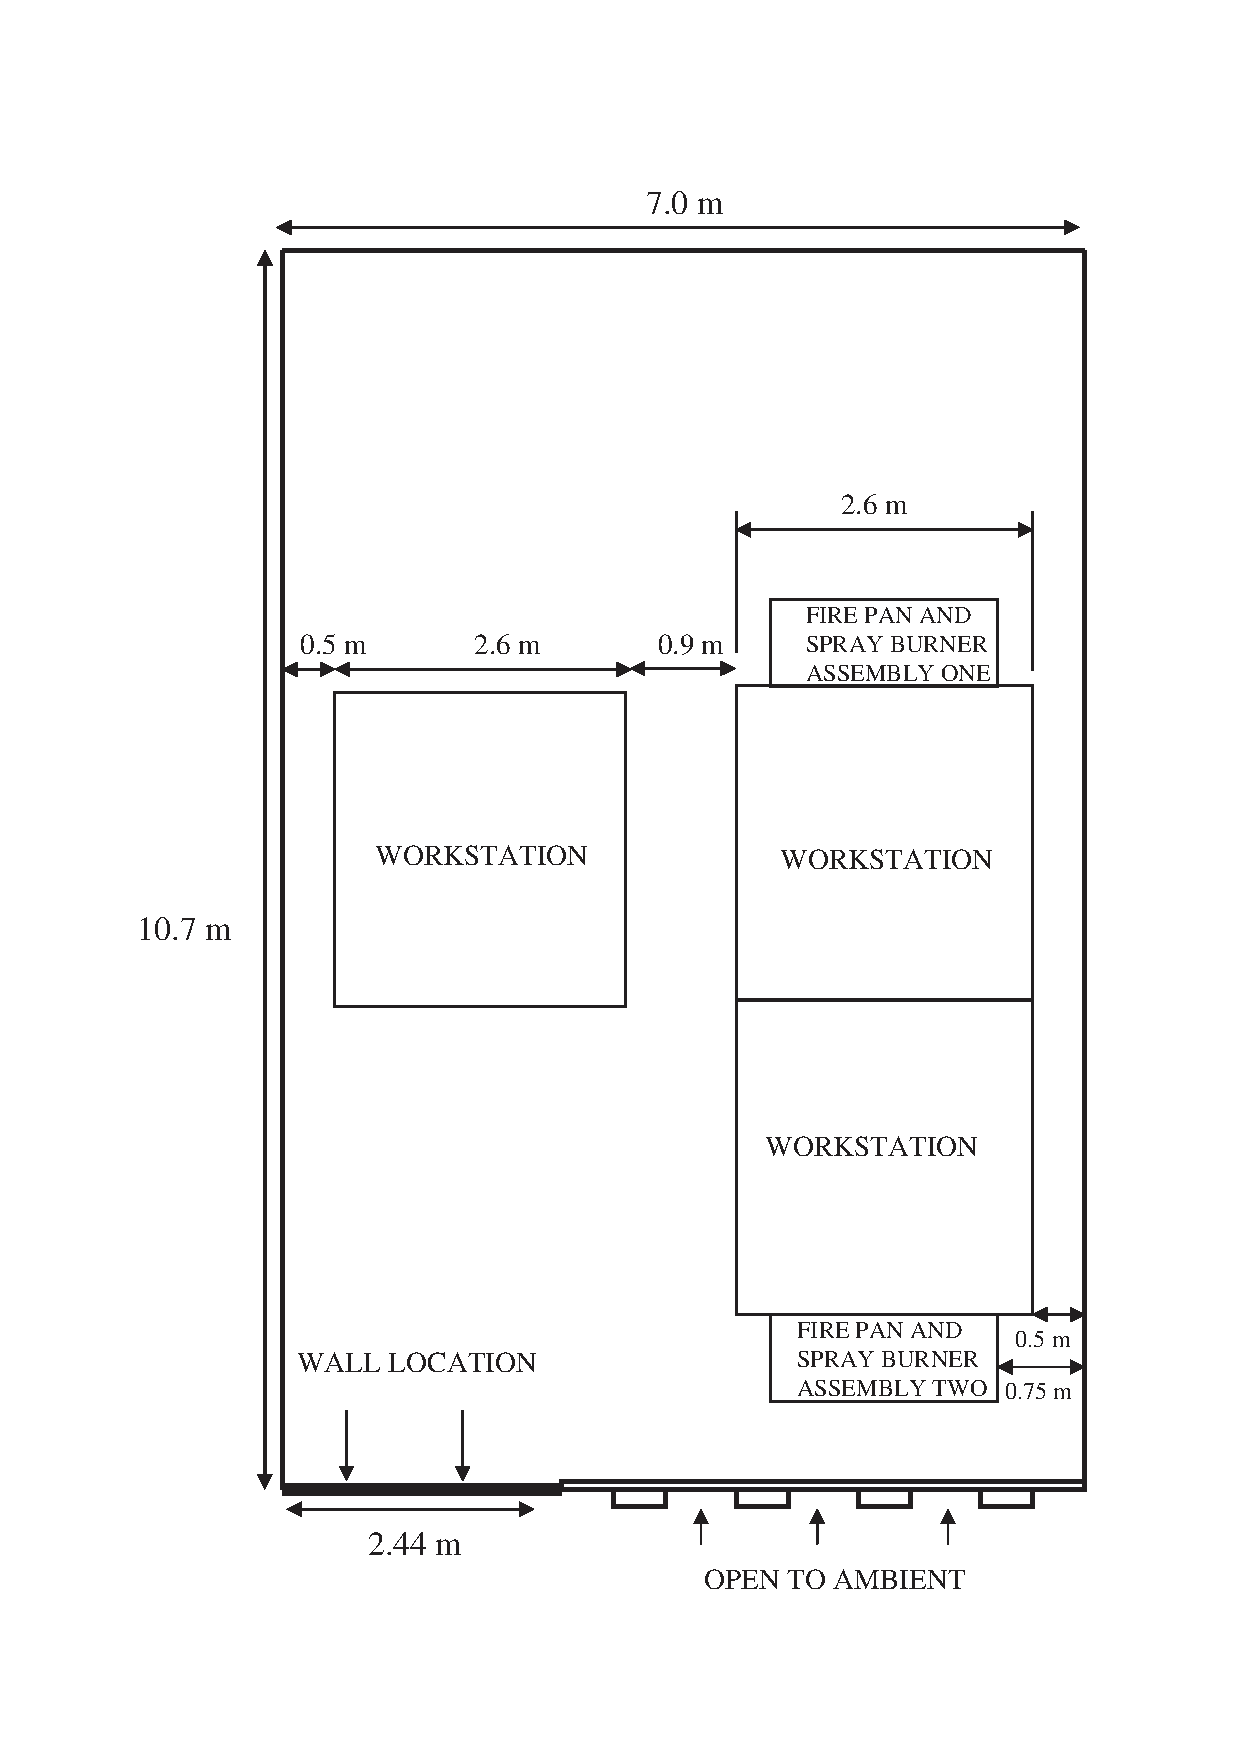
\includegraphics[width=6cm,height=10cm]{manzello_compartment}		
		\caption{Compartment dimensions used by \citet{Manzello2005}}
			\label{fig:manzello_compartment}

	\end{figure}

Thermocouples were attached throughout the compartment and the time-temperature plot was recorded. Infra-red cameras along with normal cameras were used to investigate the crack pattern in the unexposed face of the wall. Heat flux sensors were also used to measure the flux on the surface of the plasterboards at four locations on the unexposed face of the wall partitions. It was observed that the rate of temperature rise on the plasterboard surfaces was higher when compared to the same specimens when tested in the furnace. It was also reported that the total heat flux measured was dependent on the height of the wall. But the rate of increase of the heat flux was smaller when compared to the furnace fire test. Numerical modelling for the experiments conducted were also performed by \citet{Manzello2007}. The model was entirely mathematical instead of widely used FE modelling. It was then concluded that the proposed mathematical model could predict the fire behaviour only upto certain level of precision as there were several effects such as smoke movement during fire, plasterboard fall-off etc. 

\citet{Sultan2006} investigated the effect of furnace depth in fire tests on wall and floor assemblies using incident heat flux measurements. This included the furnaces used for intermittent and full -scale fire tests. The heat flux incident on the surface from furnace is investigated with the help of 12 fire tests. It was observed that the heat flux measurements from floor tests were slightly larger than that of the wall tests. The heat flux in the intermitent-scale wall furnace was significanlty higher than the full-scale wall furnace when the CAN/ULC-S101 or ASTM E119 time–temperature curve was used. The heat received by a test specimen in furnace is through convection and radiation, where radiation plays a major role followed by natural convection in full-scale furnace. Whereas, in small-scale furnace, the heat transfer is preceded through forced convection as the burners being close to the test specimen. Increase in furnace size decreases the heat transfer through forced convection, thereby radiation dominating the heat transfer process resulting in decreased heat flux in small-scale furnaces. The difference in heat flux due to the orientation of the furnace was considered to be less significant. 

\citet{Kodur2006} investigated the important factors that influenced the resistance of load bearing steel stud walls. Spacing of the studs in the panel, thickness of the steel used, the magnitude of load acting on the panel, shear membrane and type of installation were the parameters analysed in this research. It was found that the insulation type and the number of layers of gypsum board in the panel were highly influential for fire resistance of steel stud wall assemblies. Also, the fire rating of the wall assemblies without cavity insulation was higher in comparison with the wall panels possessing cavity insulations. Increasing the layers of plasterboard resulted in higher fire resistance for the entire wall system rather than using a single plasterboard. Provision of the OSB shear membrane in place of gypsum boards in load bearing wall panels resulted in deterioration of the fire resistance. Studs arranged in a staggered manner in two rows resulted in higher fire resistance when compared to a single layered stud arrangement. It was discussed that this higher fire resistance of the double layered staggered stud arrangement was due to the larger heat sink because of larger cavity within the wall. Another finding was that MSG 20 light steel section performed better than ordinary MSG 20 section in providing fire resistance.

\citet{Knobloch2006} proposed a strain based approach to local buckling of steel sections exposed to fire. Generally, the stress based design approach based on ambient temperatures is used to design the cold-formed steel sections. Unaltered effective width and the yield strength reduced to 0.2\% proof strain were only used for design. This has resulted in unsatisfactory design results. Hence strain based method to design cold-formed steel sections was developed for unstiffened and stiffened elements in a member. Strength curve based on yield line theory considering the initial imperfection was also formulated. Calculations are done based on the proposed design methods and compared with the results from the numerical analysis. It is to be noted that the non-linear material behaviour was also considered in the proposed method. The procedure involved in this proposed design is as follows. 
\begin{itemize}
	\item For different support conditions the non-dimensional slenderness   at elevated temperature is determined.
	\item Then the reduction factor $\rho\theta$  is calculated based on \citet{Desmond.1981},  also known as Winter’s equation as shown next.
	\begin{equation}
	\rho \theta = \dfrac{1}{\bar{\lambda}_{\rho \theta}}\Bigg(\dfrac{1-0.22}{\bar{\lambda}_{\rho \theta}}\Bigg) 
	\end{equation}
	\item Later the effective width is calculated using the proposed stress-strain relationships at elevated temperatures and the stress distribution of the element is obtained.
	\item Finally, the axial and bending moment resistances are calculated by integration.
\end{itemize}

The proposed effective width formula for unstiffened and stiffened elements are as shown in \Cref{fig:knobloch_effwidth}.

\begin{figure}[htbp]
	\centering
		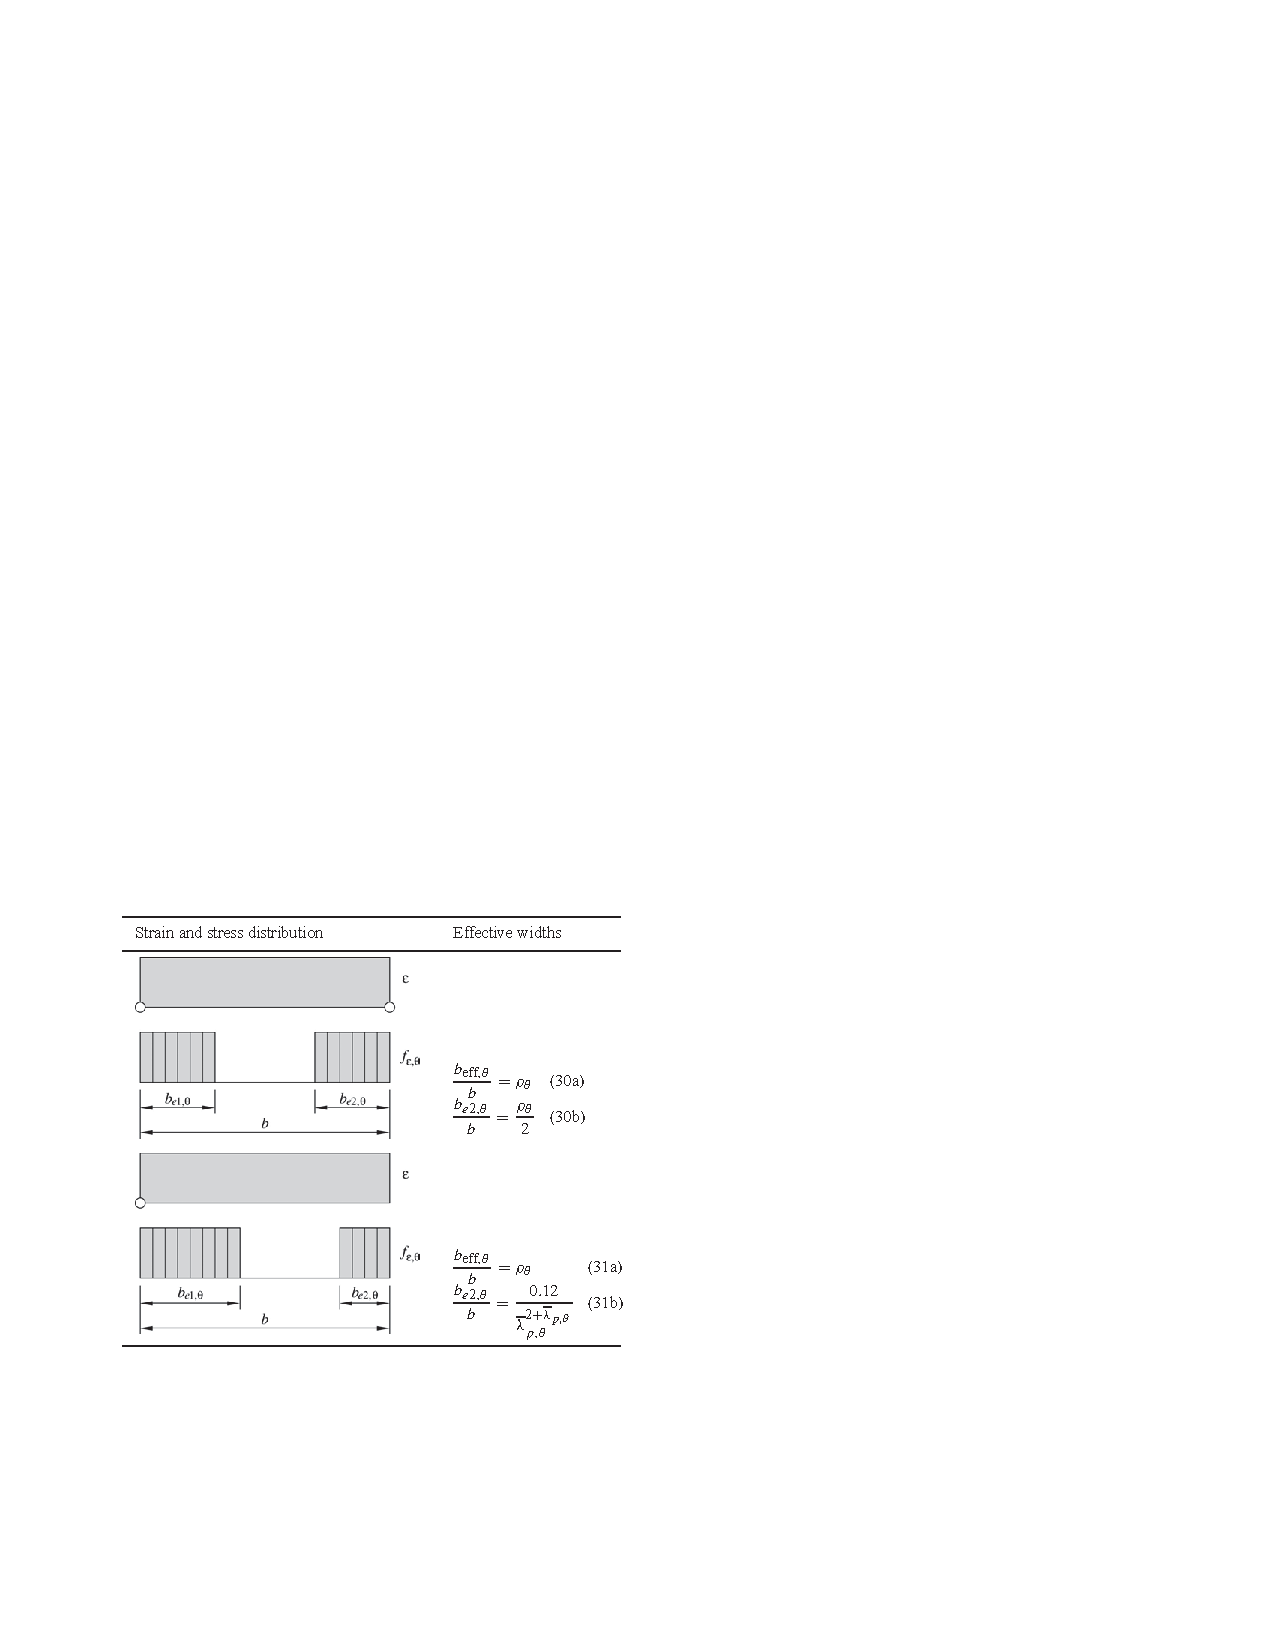
\includegraphics[width=10cm,height=10cm]{knobloch_effwidth}		
		\caption{Proposed effective width table from \citet{Knobloch2006}}
			\label{fig:knobloch_effwidth}

	\end{figure}

It was concluded that, the local buckling of the studs and the additional capacity due to the plastic behaviour of cross section had a strong influence on the resistance of the steel under fire. Also, the local buckling was dependent largely on the strain. 

Experimental investigation of different cold-formed steel materials at elevated temperatures were conducted by \citet{Chen2007}. Primary focus of this research was to report the material properties of cold-formed steels at elevated temperatures. Tensile coupon tests at elevated temperatures for G550 and G450 grade steel with varying thickness were conducted to determine the elastic modulus and yield strength at different strain levels, ultimate strength, ultimate strain and thermal elongation for comparison with Australian, British and Eurocode Standards. A unified equation to predict the above mentioned physical properties was also proposed. Comparison between the test results and proposed equations were also carried out. Tensile tests were carried out in MTS Model 653 with temperature capacity up to 1400\degree C. Thermocouples were used on the internal and external faces of the specimen to record the time-temperature pattern. Both transient and steady state methods were used in the tensile coupon tests. But the transient method is more practical in real time fire exposure. Differential thermal analysis was used to investigate the chemical reactions which happens within the steel during fire exposure. Yield strengths at 0.5\%, 1.5\% and 2\% strain levels were obtained and comparison among them was undertaken. Serration was observed on the stress-strain curve at high temperatures. Static drop was obtained in the stress-strain curve at room temperature of 22\degree C. This was achieved by pausing the strain applied for 1 minute thereby allowing the stress relaxation associated with plastic strain. This reduces the effect of loading rate. A series of tests were also conducted to study the effects of static drop at different temperatures. Based on the experimental investigations, an equation for determining yield strength, ultimate strength and ultimate strain of cold-formed steels was proposed as follows.

\begin{equation}
\text{Yield Strength} \to \dfrac{f_{0.2,T}}{f_{0.2,normal}} = a-\dfrac{(T-b)^{n}}{c}
\end{equation}

\begin{equation}
\text{Ultimate Strength} \to \dfrac{f_{u,T}}{f_{u,normal}} = a-\dfrac{(T-b)^{n}}{c}
\end{equation}

\begin{equation}
\text{Ultimate Strain} \to \dfrac{\epsilon_{u,T}}{\epsilon_{u,normal}} = a-\dfrac{(T-b)^{n}}{c}
\end{equation}

A modified stress-strain curve model based on the Ramberg-Osgood model was proposed as follows.

\begin{equation}
\epsilon_T = \dfrac{f_T}{E_T}+0.002\big(\dfrac{f_T}{f_{y,T}}\big)^{nT} for f_T \leq f_{y,T}
\end{equation}

\begin{equation}
\epsilon_T = \dfrac{f_T-f_{y,T}}{E_{y,T}}+\epsilon_{u,T}\big(\dfrac{f_T-f{y,T}}{f_{u,T}-f_{y,T}}\big)^{mT} + \epsilon_{y,T} for f_T > f_{y,T}
\end{equation}

Where

\begin{equation}
E_{y,T} = \dfrac{E_T}{1+0.002n_TE_{y,T}/f_{y,T}}
\end{equation}

\begin{equation}
n_T = 20-0.6\sqrt{T}
\end{equation}

\begin{equation}
m_T = 1+\dfrac{T}{350}
\end{equation}


From this study, it was concluded that the Australian, British and European standards were conservative in predicting the yield strength, elastic modulus and thermal expansion except for G550 1 mm steel between 450\degree C to 970\degree C and for G450 1.9 mm steel at 600\degree C. The proposed equations predicted the yield strength and elastic modulus of the cold-formed steel more accurately at higher temperatures than the standards mentioned above when compared with the experimental results. Also, the ultimate strengths and strains for the cold-formed steel calculated by the proposed equations at high temperatures showed a good agreement with the test results.

\citet{Cooke2008} investigated the collapse of steel faced sandwich panel walls and ceilings exposed to fire. In this investigation, the overall structural stability of the sandwich panels, ceilings and firewalls exposed to fire on one side was investigated. The computation of catenary force required in resisting the collapse of the panel during delamination when exposed to fire, due to softening of adhesive and mid-span deflection were the key focus of this investigation. The catenary force equation was given as 

\begin{equation}
H = \dfrac{wL^{2}}{8D}
\end{equation}

Where
\begin{description}[itemsep=0pt,parsep=0pt]
	\item H = Horizontal restraint force,
	\item w = Distributed load per unit length,
	\item L = Span,
	\item D = Deflection.
\end{description}

\citet{Kolarkar2008} studied the thermal performance of LSF walls with double layer plasterboards, where the insulation was sandwiched between the plasterboards externally. The investigation was carried out by conducting small-scale fire tests of non-load bearing LSF walls exposed to the standard fire curve from AS 1530.4. It was found that the sandwiching of insulation externally between the plasterboards resulted in better thermal performance when compared to traditional stud walls with cavity insulation. 

\citet{Ranawaka2009} investigated the distortional buckling behaviour of cold-formed steel compression members at elevated temperatures. Lipped and Unlipped channel specimens were tested under compression loading at temperatures ranging from 20 to 800\degree C. The ultimate compression capacities of these sections from the tests were compared with design code predictions. The distortional buckling capacities from the tests were compared with that of direct strength and buckling strength equations in AS 1530.4 and were found to agree well at ambient temperature. At elevated temperatures, the reduced mechanical properties were used to predict the compression capacities which were compared with the test results. This comparison showed that the design equations in AS/NZS 4600 were over-conservative.

The usage of proper instrumentation is essential in recording temperature data during fire test. Therefore \citet{Sultan2010} investigated the different temperature censors and their performance during fire tests. This research included the sensors such as ASTM E119 Shielded Thermometer, ISO 834 Standard Plate Thermometer, Directional Flame Thermometer, Bare-Bead Thermocouples, Ground Sheathed Thermocouples and Ungrounded Sheathed Thermocouples. Other measurement devices considered for investigation includes Heat Flux Sensor and Furnace Cover. It was found that the Bare-bead thermocouples had the least lag in response time for temperature measurement. However, the difference in temperature lag with other sensors became insignificant after 10 min of fire test. This was due to the accuracy in measuring the convective heat transfer in the initial stages of fire tests. At higher temperatures at later part of the fire test the convective heat transfer becomes negligible. It was also reported that rapid temperature rise in a furnace is easier to control in a deeper furnace rather than a shallow furnace.

\citet{Rahmanian2011} conducted 12 medium-scale (1m $\times$ 1m) fire tests on LSF walls under load bearing conditions. Standard cellulose fire curve based on BS476 (BSI, 1987) was used for the fire tests. The number of plasterboard layers were varied to study the thermal behaviour of gypsum plasterboard assemblies using different types of plasterboards. The concept of cyclic condensation-evaporation of the moisture content in the plasterboard during fire tests were also investigated. Material property tests were also conducted on various gypsum plasterboards to study the effect of moisture transfer in gypsum plasterboard assemblies and the data was used to develop thermal finite element models in ABAQUS. 

\citet{Chen2012a} conducted five full scale fire tests of conventional single stud LSF wall systems with different plasterboards commonly available. The main aim of this research was to investigate the fire performance of loadbearing LSF walls with different plasterboard along with gypsum plasterboards. Bolivian magnesium board and calcium silicate boards were used for this study. Load ratios of 20\%, 40\% and 70\% were considered for the load bearing fire tests. It is to be noted that the load bearing LSF walls without cavity insulation provided better FRL when compared to LSF walls with cavity insulation. Also, the thickness of the stud section influenced the FRL. Thicker the stud higher was the FRL. This effect was reported by previous researchers also. It was concluded that the calcium silicate boards when used in the base layer provided better fire performance when compared to gypsum plasterboards. However due to the spalling behaviour of calcium silicate boards at higher temperatures, it does not possess a noticeable advantage when compared to gypsum plasterboards. Bolivian magnesium oxide plasterboards perform better in fire when compared to gypsum plasterboards. Staggered arrangement of boards were followed in the fire tests, but there were no significant changes in the steel temperatures when compared with conventional plasterboard arrangement. 

\citet{Kolarkar2012} investigated the fire performance of LSF walls experimentally using small-scale fire tests. Total of nine small-scale tests were conducted which was exposed to ISO 834 standard time-temperature curve. A novel LSF wall configuration of external insulation was introduced and the fire performance of the same was also investigated using small-scale fire tests. The test wall dimensions were 1280 mm $\times$ 1015 mm. Insulation materials such as glass fibre, rock wool and cellulose were considered for this research study. The following findings were drawn from this research.
\begin{itemize}
	\item Presence of plasterboard joints did not significantly affect the thermal performance, in comparison with test wall specimen without plasterboard joints in small-scale fire test. However, the plasterboard joints can have significant effect in full-scale fire tests and under load bearing conditions.
	\item LSF test walls with single plasterboard configurations tend to exhibit steep rise in temperatures as the plasterboard calcinates after 20 min of fire test. This leads to premature structural failures in LSF walls under load-bearing conditions when exposed to fire.
	\item Heat transfer on the studs in non-cavity insulated LSF walls was more uniform in comparison with cavity insulated LSF walls resulting in reduced thermal bowing of the LSF wall.
	\item The studs of LSF walls with rock fibre insulation resulted in higher temperatures on the hot flanges while the stud temperatures of LSF walls with cellulose insulation were the lowest. This indicates that the non-uniformity in temperature distribution is highest in LSF walls with rock fibre insulation and can result in premature structural failures under load-bearing conditions.
\end{itemize}

\citet{Gunalan2013e} investigated experimentally the behaviour of load bearing LSF wall systems exposed to ISO fire curve. Eleven full scale fire tests with test specimens of 2.4 $\times$ 2.4 m were used as shown in \Cref{fig:gunalan_experiments}. This research focused on the LSF walls used in Australia. Conventional LSF wall assemblies with single row of studs were used in this research. The LSF wall panel arrangement was made of four studs connected by tracks on top and bottom. Noggings were not used in any of the wall panels. The wall panels had different kinds of insulation such as glass fibre, rock fibre and cellulose fibre. Next generation LSF panels by sandwiching insulation between the plasterboards were developed as a part of this research. The studs used were 92x40x15x1.15 (G500) lipped channel sections. Load ratios of 0.2 and 0.4 were used (9 and 2 tests). 
\begin{figure}[!htbp]
	\centering
		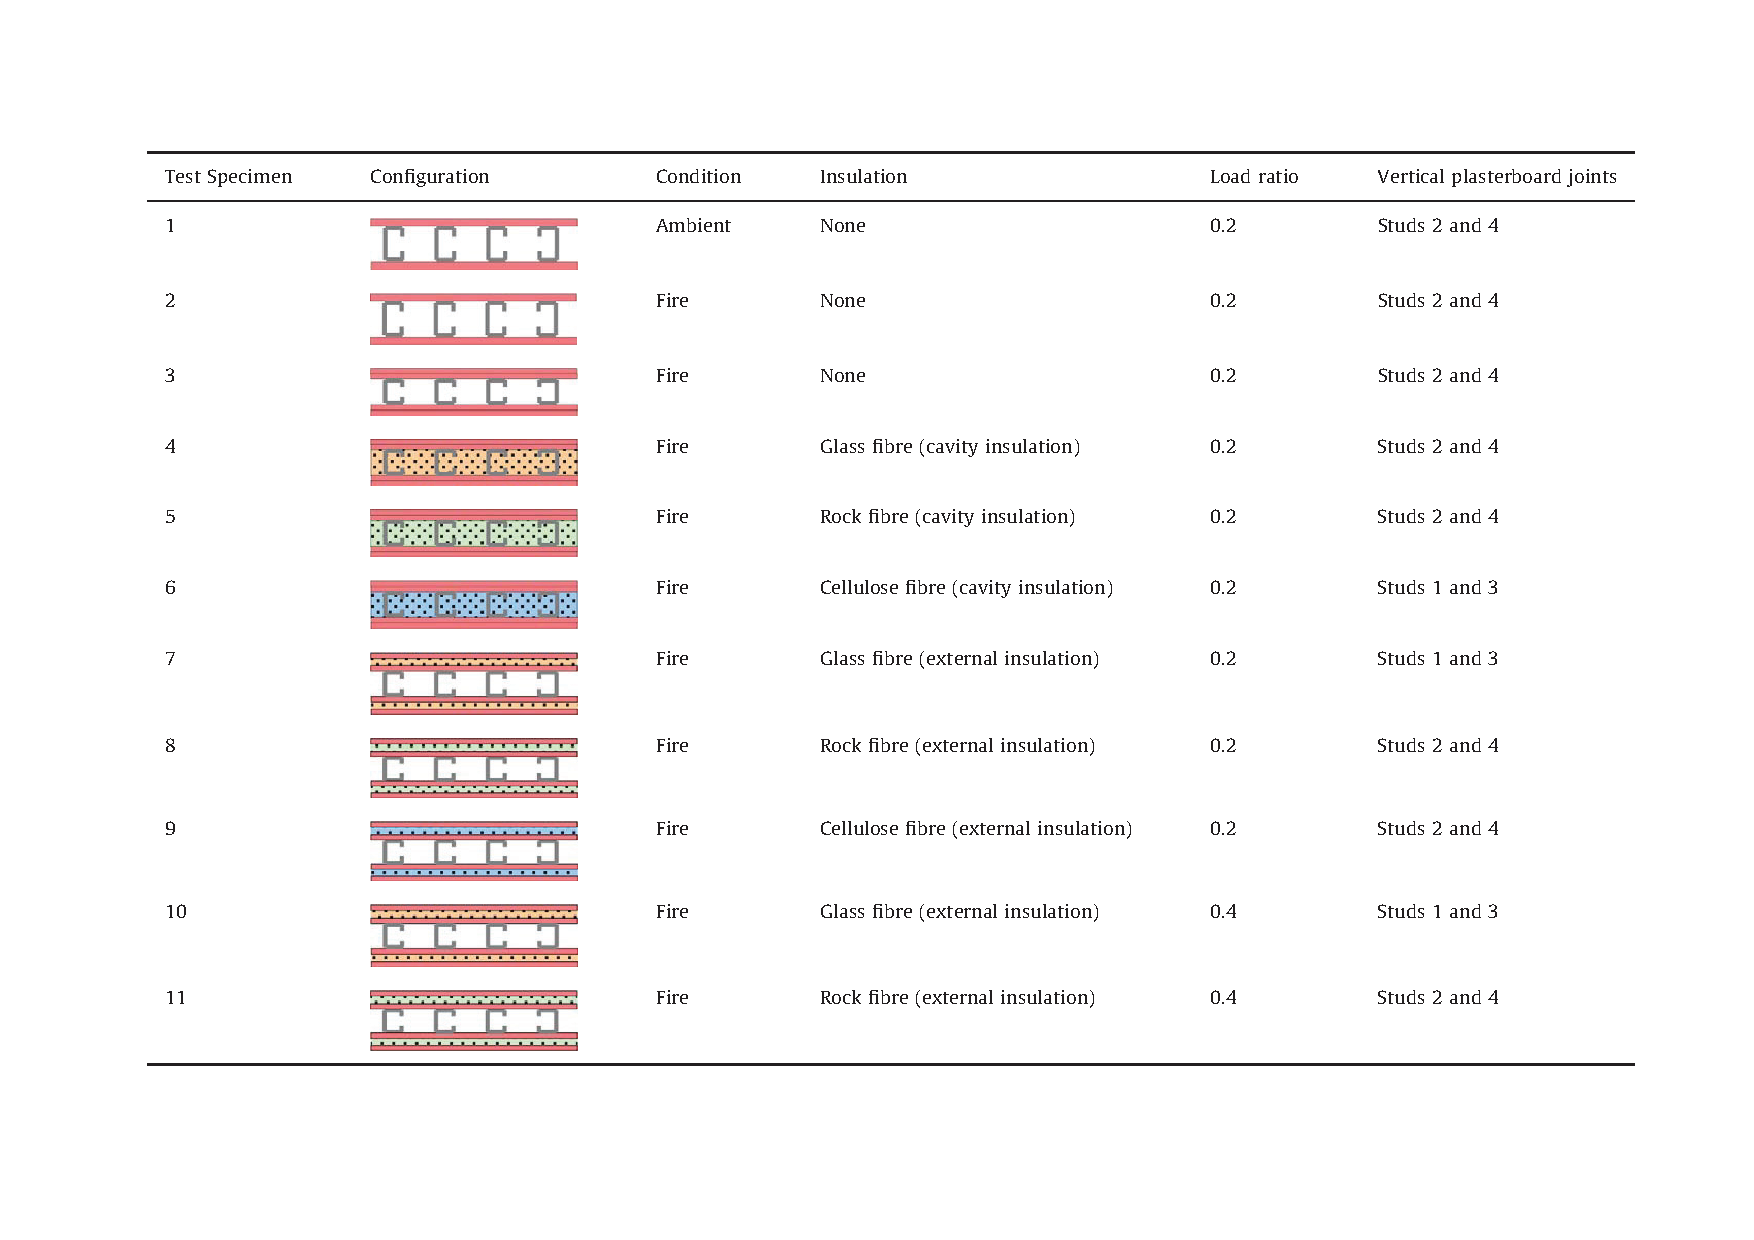
\includegraphics[width=14cm,height=10cm]{gunalan_experiments}		
		\caption{Test wall configurations used by \citet{Gunalan2013e}}
			\label{fig:gunalan_experiments}
	\end{figure}

Number of plasterboard layers was varied and external insulation was also used. It was found that providing external insulation in the load bearing LSF walls, significantly improved the FRL of the wall system even at higher loads.  

\citet{Chen2013} investigated different types of plasterboard and insulation materials to improve the fire performance of load-bearing LSF wall systems. Plasterboard types such as gypsum plasterboard, oriented standard boards (OSB), bolivian magnesium board, rockwool boards and autoclaved lightweight concrete (ALC) boards were used for this research. Aluminium silicate insulation was also used for the full-scale fire tests. Total of six full-scale fire tests were conducted for this research. The experimental setup included lipped channel sections with stud depth varying from 89 to 140 mm. Back to back lipped channel stud sections were used in fire tests with higher load ratios. Typical failure of studs in the test wall after fire test is shown in \Cref{fig:chen2013_test} below. 
\begin{figure}[htbp]
	\centering
		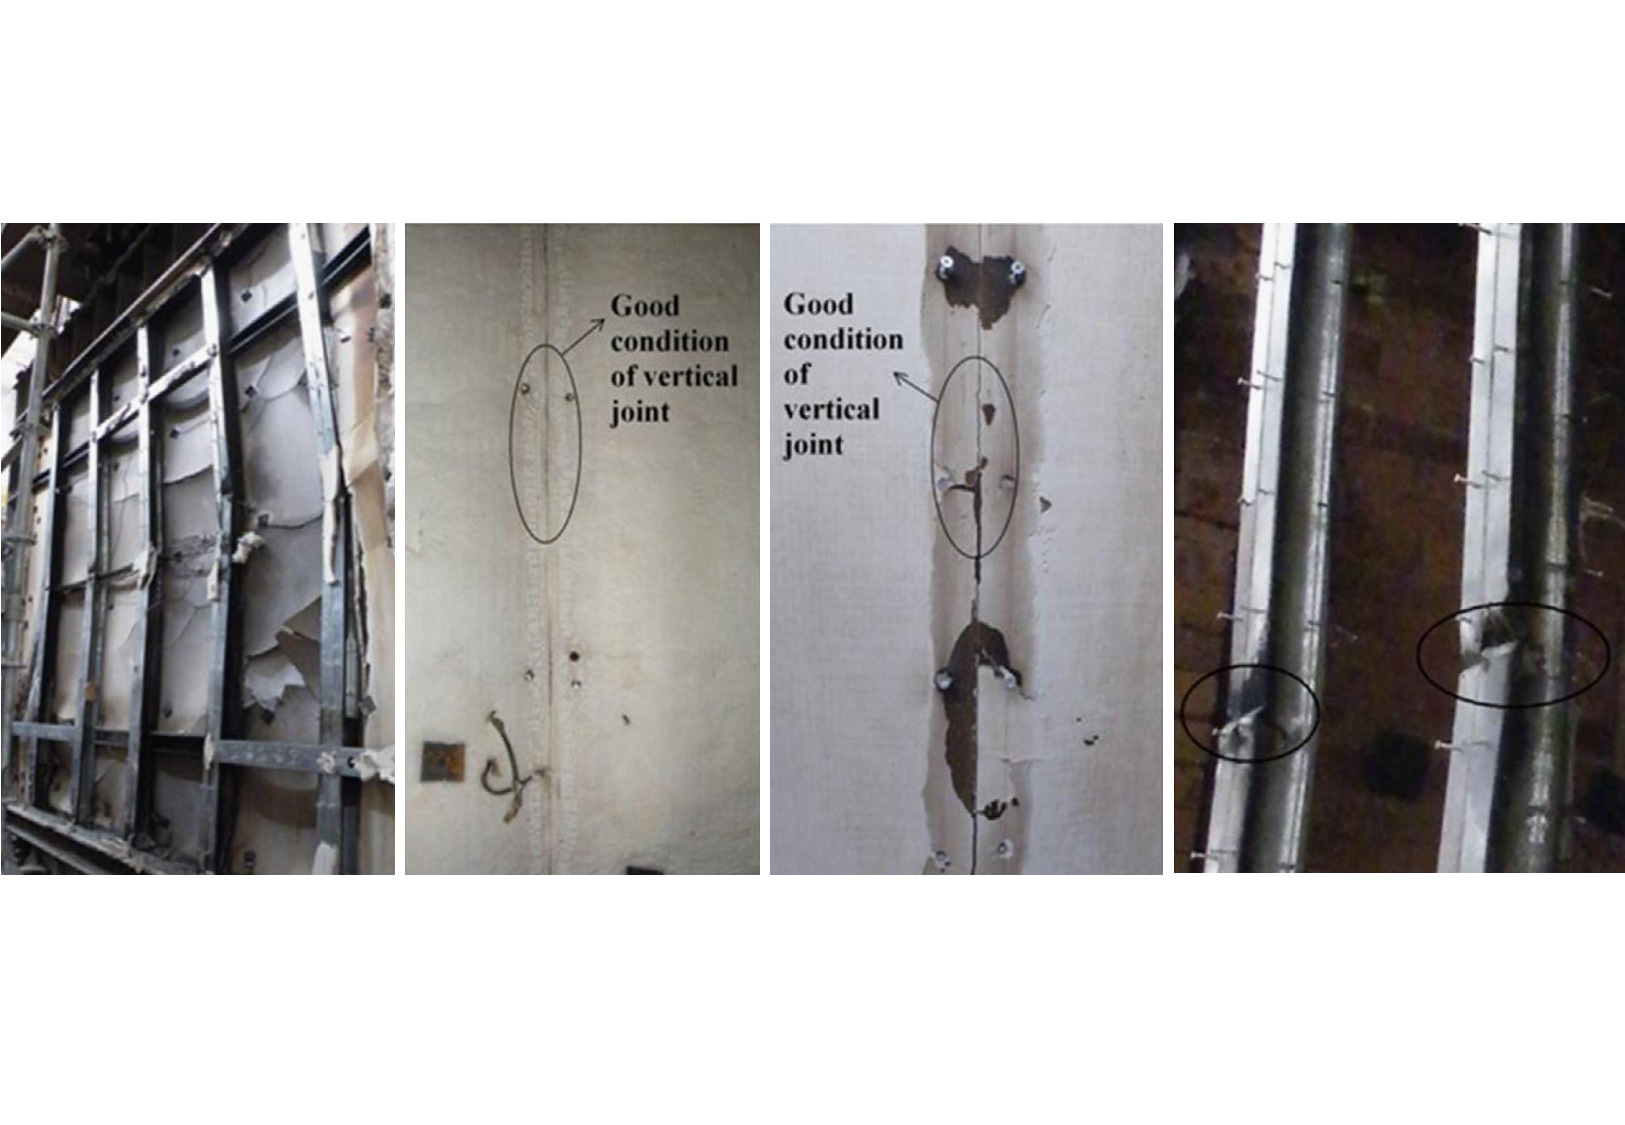
\includegraphics[width=14cm,height=5cm]{chen2013_test}		
		\caption{Lipped Channel Studs (LCS) failure in fire test conducted by \citet{Chen2013}}
		\label{fig:chen2013_test}
\end{figure}
The novel findings from this research showed that the FRL will decrease with increase in load ratio. The failure modes of the studs in test wall with bolivian magnesium board will be different in comparison with other type of lining boards. Gypsum boards and bolivian boards were found to be less suitable for use in external walls due to their durability, whereas ALC boards are preferred to be used in external walls. Increased screw-to-panel edge distance can reduce the collapse of boards thereby preventing board open up on the fire side and cracks on the ambient side. 

\citet{Kolarkar2014} investigated the fire performance of gypsum plasterboards and composite panels. Fifteen small scale tests with 13 and 16 mm plasterboards were considered in their experimental investigation. External insulations such as glass fibre, rock fibre and cellulose fibre insulations with different thickness and density were used in the small scale LSF wall panels and their fire performance was investigated. It was found that, the composite wall panels in which the insulations were provided externally, performed better under fire exposure when compared to wall panels with cavity insulations. Another important observation is that the glass fibre insulation disintegrates at about 700\degree C which is achieved at about 50 minutes of fire exposure resulting in premature failure of the walls with cavity insulation when compared with walls without cavity insulation. The cellulose fibre insulation resulted in better fire performance, provided low density cellulose is used in spraying of the insulation within the cavity. Also, the process of spraying cellulose insulation within the cavity is always not uniform and was suggested to arrive at varying results. Out of all the combinations used in this research, the rockwool external insulation was found to withstand disintegration better when compared with its counterparts. This is because the rockwool insulation did not disintegrate till the end of fire test, whereas the insulation materials disintegrated easily which ultimately reduced the FRL. 

\citet{Ariyanayagam2014e} studied the thermal performance of LSF walls under realistic design fires. Their test results were compared with those from LSF walls tested with standard ISO fire curve. Finite element models were developed for transient and steady state analyses and the results were compared with the test results. The FEA results for the design fire curve were in good correlation with the experimental results. This research illustrated the difference between the effects caused by a standard fire and a realistic design fire in buildings. It also emphasized the use of realistic fire curves for the design of LSF walls.  The effects of plasterboard joints and their arrangements were also investigated experimentally. It was observed that back blocking plasterboard joint arrangement used over the studs increased the FRL of LSF walls significantly by 25\% when compared with the traditional plasterboard joints. Numerical studies were also carried out to validate these results and were found to be in good correlation with experimental results. 

\citet{Kesawan2015} proposed the usage of welded hollow flange channel (HFC) sections in LSF walls. HFC sections have two flanges connected to the web through welding as shown in below. 
\begin{figure}[htbp]
	\centering
		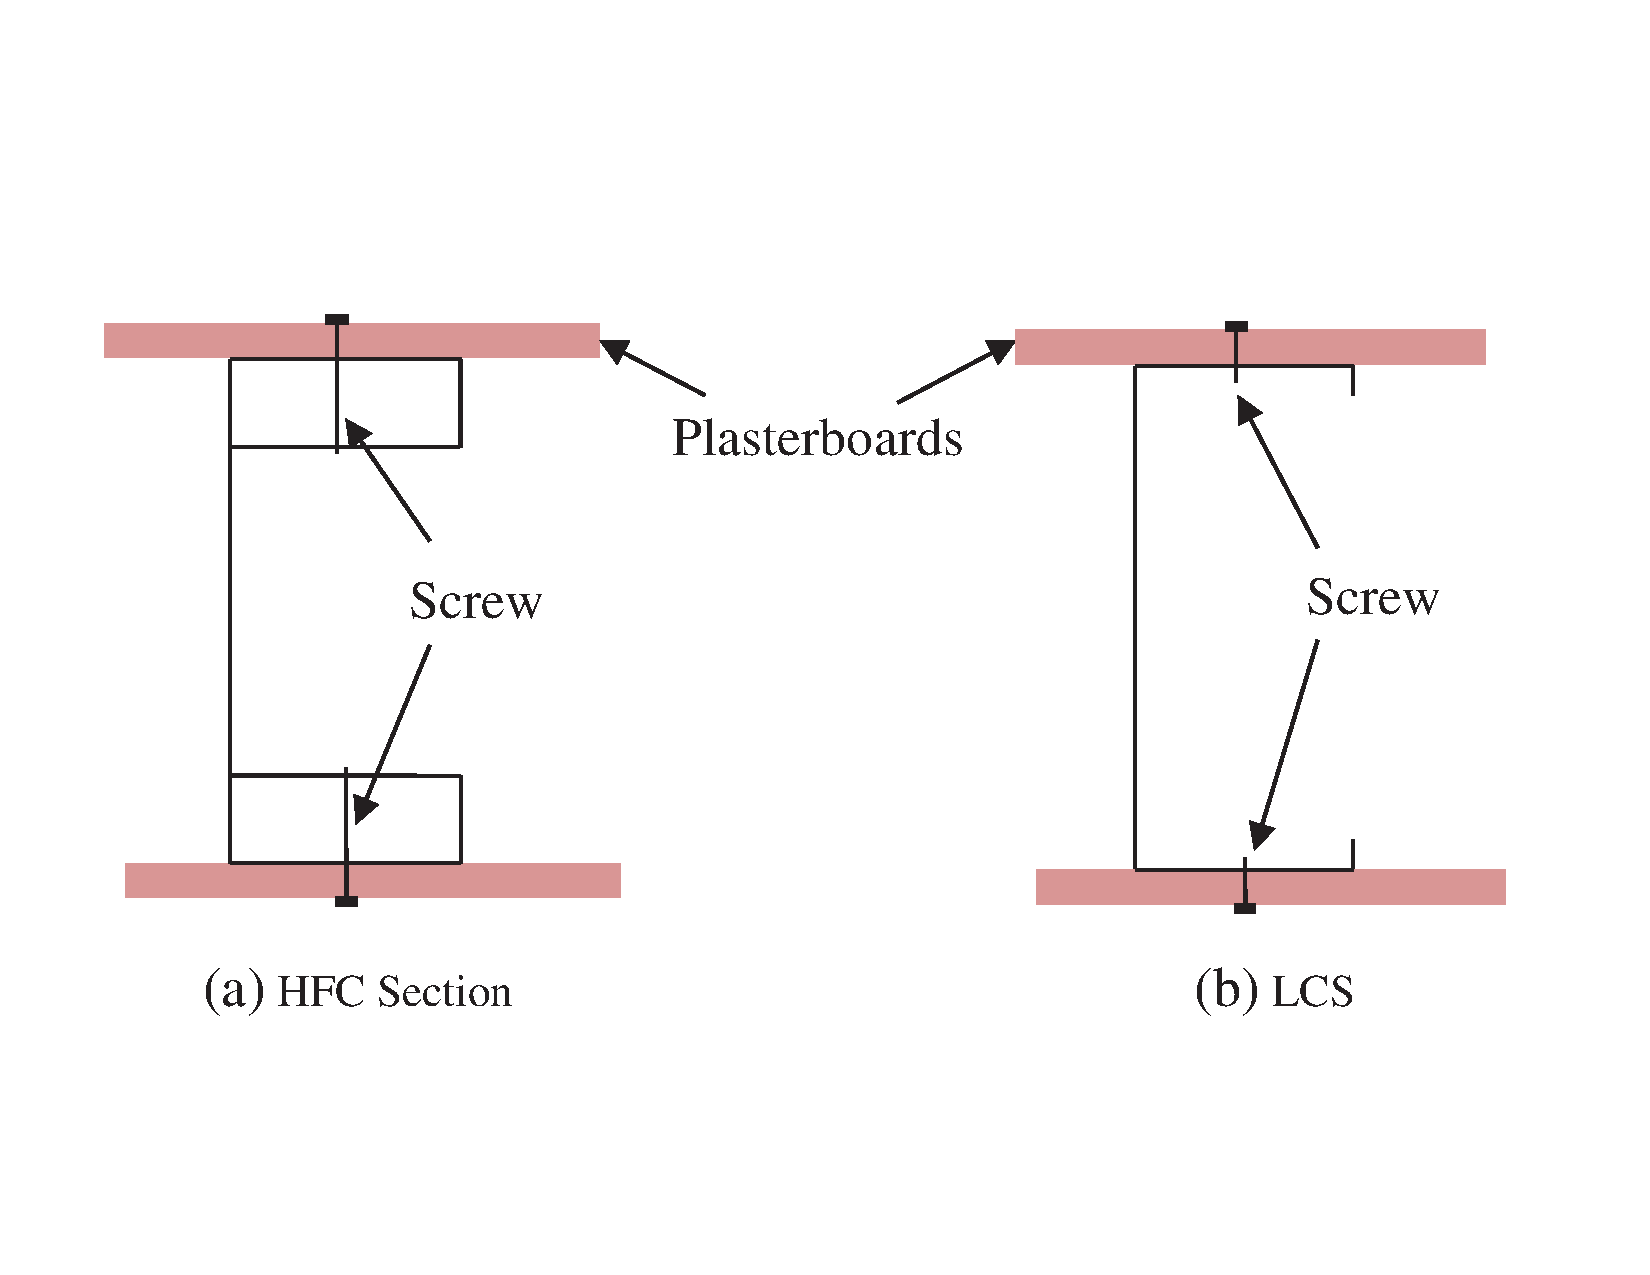
\includegraphics[width=10cm,height=5cm]{kesawan2015_section}		
		\caption{Hollow Flange Channel (HFC) studs used by \citet{Kesawan2015}}
		\label{fig:kesawan2015_test}
\end{figure}
Investigations were carried out on LSF walls with hollow flange channel sections to determine the thermal performance of LSF walls in fire. Initially the mechanical properties of the flange and web elements of the hollow flange channel sections were determined by tensile coupon test at elevated temperatures. Secondly, full-scale fire tests of load bearing LSF walls with hollow flange channel studs were conducted. New parameters such as specific heat, density, emissivity and enthalpy were proposed for the thermal FE modelling of this new LSF wall configuration. The experimental investigation was carried out for various profiles of the hollow flange channel sections with and without insulations. Numerical models were created with measured mechanical properties and validated by comparing the results with experimental results. Parametric study was conducted by varying the section geometry and stud thickness. Their results showed that the FRL was not improved by the stud section geometry, provided the section depth and thickness remains the same. 

\citet{Rusthi2017b} conducted full-scale fire tests in LSF walls using Australian Magnesium Oxide (MgO) boards instead of the conventional gypsum plasterboards with lipped channel steel sections. This research investigated the thermal properties of the MgO boards in detail followed by full-scale fire tests. All the fire tests were conducted under non-load bearing conditions. Total of three full-scale fire tests were conducted as part of this study, which included, LSF walls with and without cavity insulation. Significant cracking sound was noticeable with cracks on the ambient side after 25 min of fire test. Heavy delamination and cracking of MgO boards was noticeable on the fire exposed side after the fire test. Integrity based failure was the mode of failure in all fire tests. Despite the usage of mortar in board joints that can withstand high temperature, the cracking of the joints during fire test could not be nullified in this research. It was also found that the usage of noggings in LSF walls with MgO boards, resulted in more cracking in comparison with wall assemblies without noggings. Therefore, it was recommended to exclude noggings in LSF walls subjected to large deformations.

\citet{Rusthi2017} developed heat transfer models in ABAQUS to predict the thermal behaviour of LSF walls under fire. 3D solid heat transfer brick elements were used for steel studs and plasterboards to create the heat transfer model. Tie constraints were used in the model to fix the steel studs and plasterboards for the heat transfer analysis. Five different LSF configurations were considered for the purpose of validation. Limiting hot flange temperatures proposed by \citet{Gunalan2013e,Ariyanayagam2014e} were considered for the parametric study to arrive at failure time of the considered LSF wall configurations. The limiting hot flange temperatures in LSF walls were found to be decreasing with the increase in load ratio. The boundary conditions for the heat transfer model includes the following.
\begin{itemize}
	\item ISO 834 standard time-temperature curve on the fire exposed side of the model.
	\item The model was enclosed on all the sides and cavity radiation was specified within the cavity with an emissivity co-efficient of 0.9.
	\item Convective film transfer coefficient of 10 $W/m^2/$\degree C was specified on the ambient surface while 25 $W/m^2/$\degree C was specified on the fire exposed surface.
	\item Radiation was assumed to be the dominant mode of heat transfer within the cavity neglecting the effects of convection within the cavity.
\end{itemize}
Time-temperature curves were extracted from the thermal analysis and compared against the corresponding experimental results. The model predictions were found to exhibit reasonable match with the time–temperature curve from the experiments.

\citet{Ariyanayagam2018a} conducted an experimental study on the fire performance of non-load bearing LSF walls. Total of five full-scale fire tests were conducted for this research study. Gypsum plasterboard thicknesses of 13 and 16 mm were used along with 92 mm deep studs. Test wall configurations included different plasterboard layers, cavity insulation and noggings to investigate the influence of these components in the fire performance of non-load bearing LSF walls. The test results showed that the typical failure mode in the non-load bearing LSF wall fire test was through insulation criteria, where the ambient surface plasterboard temperatures exceeded the limiting temperature. Finding from the research showed that the increase in plasterboard thickness resulted in increased FRL. The presence of noggings in non-load bearing LSF walls did not significantly influence the thermal behaviour. However, this can have considerable contribution to the structural behaviour under load bearing conditions. It was also found that the melting point of the insulation material used should be higher to achieve increased FRL. 

Later \citet{Ariyanayagam2018c} investigated effects of low strength steel studs subjected to fire under load bearing conditions. Full-scale fire tests were conducted under 0.4-0.6. Material properties at elevated temperatures were obtained through experimental investigation for the low strength steel studs and parametric study was conducted using ABAQUS. Structural analysis results showed that, the usage of low strength steel resulted in reduction of FRL by 25\% in comparison with a similar LSF wall made of high strength steel. The critical hot flange temperatures were also lower due to the reduction in the mechanical properties of steel at elevated temperatures. It was found that the usage of appropriate reduction factors in FE analysis is critical in predicting the FRL through numerical methods. 

\citet{Dias2018a} conducted experimental investigation on the fire performance of LSF walls with steel sheathing under non-load bearing conditions. Small-scale fire tests were conducted on LSF wall assemblies with steel sheathing placed at various position. The test wall assemblies were 1 m $\times$ 1 m in which thin steel sheets were sandwiched between plasterboards. Sheathing was used in the internal cavity wall facing surface and also on the fire exposed and ambient surfaces. The entrapment of water molecules from gypsum plasterboard on to the steel sheets resulted in increased thermal performance under non-load bearing conditions.    
\begin{figure}[!htbp]
	\centering
		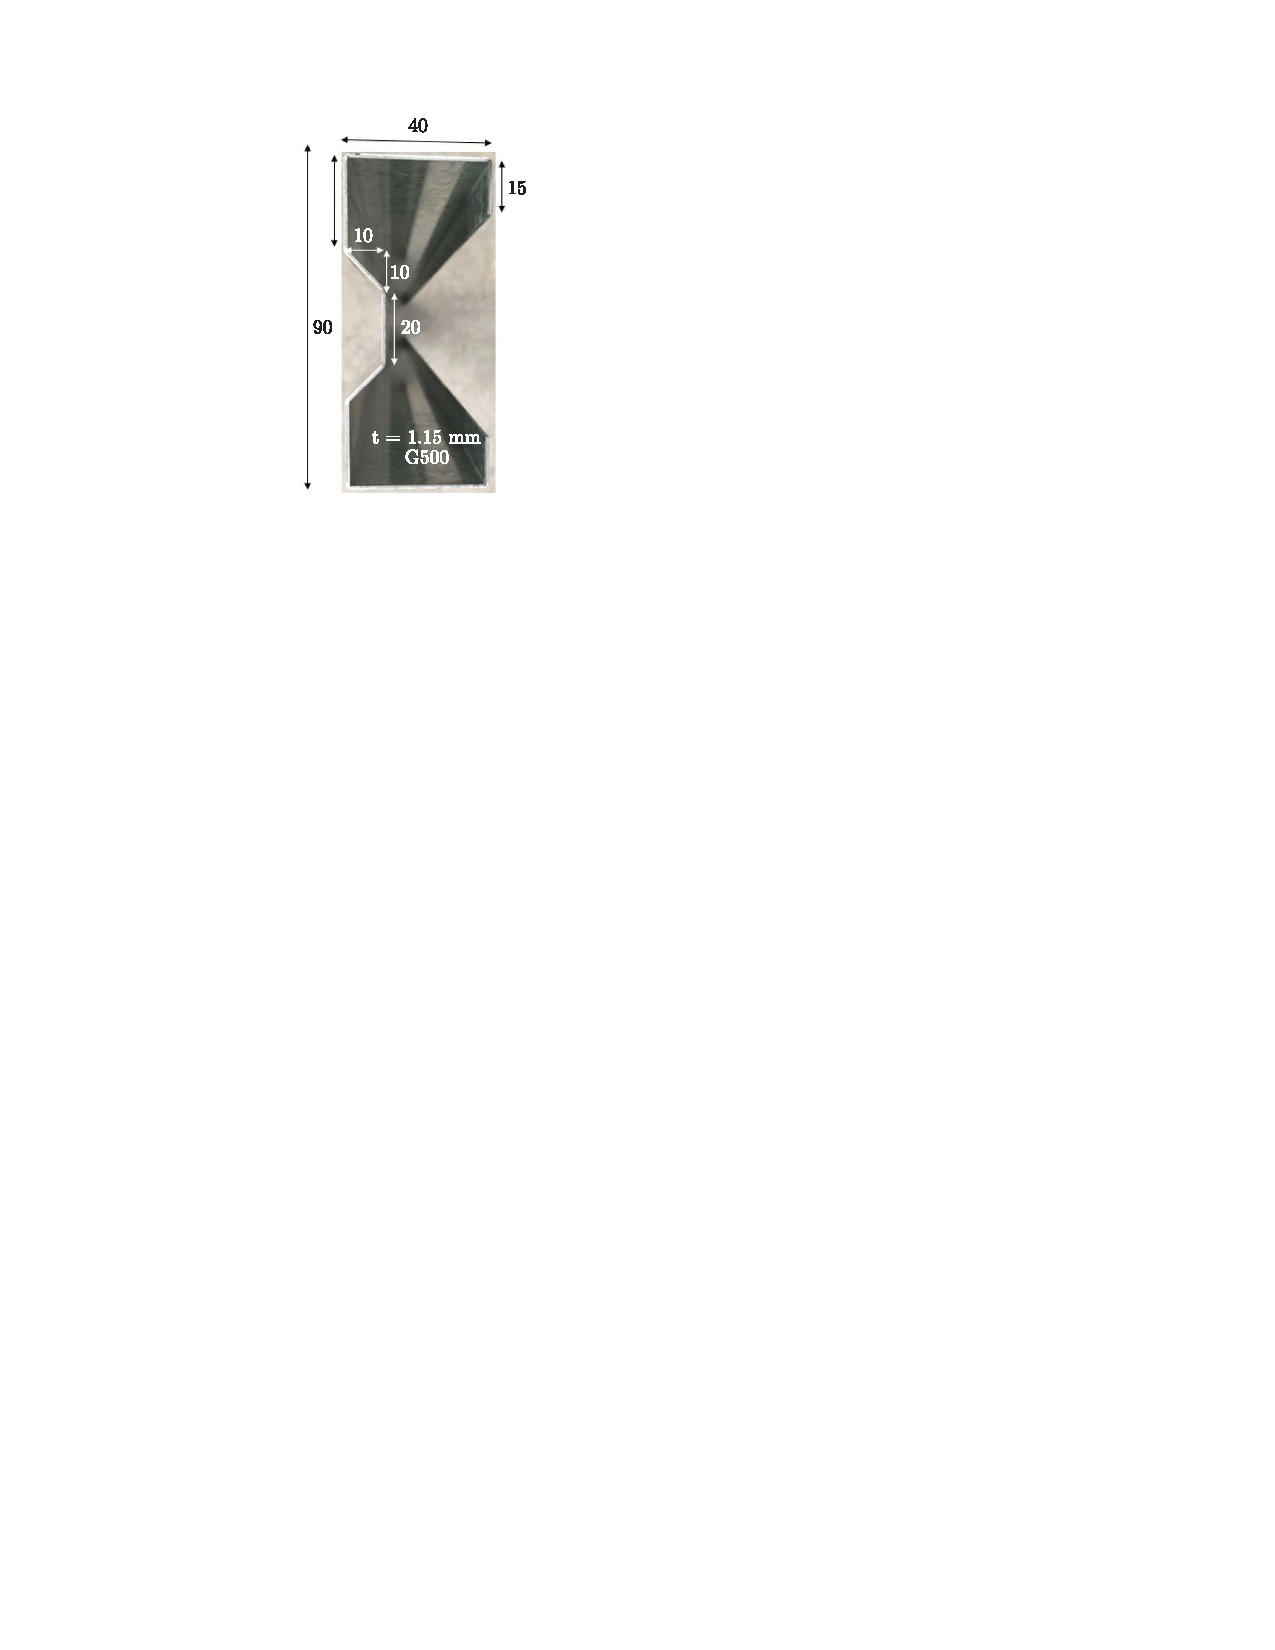
\includegraphics[width=6cm,height=7cm]{dias_stud}		
		\caption{Web-stiffened studs used by \citet{Dias2019c}}
		\label{fig:dias_stud}
\end{figure}
Later, \citet{Dias2019c} extended the investigation by conducting three full scale fire tests on LSF walls with steel sheathing. Web-stiffened studs were used instead of the conventional lipped channel sections as shown in \Cref{fig:dias_stud} below. The proposed new web-stiffened studs were able to withstand higher axial load in comparison with conventional LCS studs under ambient and fire conditions. However, when the FRL is considered based on the non-dimensional load ration, these new wall configurations were found to provide only a marginal increase in the FRL in comparison with the conventional LSF wall configuration with LCS studs.

\section{Thermal and Mechanical Properties of Cold-Formed Steels}

To study the behaviour of cold-formed steel structures under fire conditions, it becomes a necessity to account for the yield strength and elastic modulus values at elevated temperatures, as these parameters contribute to the structural strength of cold-formed steel members. The mechanical properties that are used in the research and design of cold-formed steel sections were based on BS EN 1993-1-3: (2006) and is detailed in \Cref{tab:eurocode_reduction}. These mechanical properties with the corresponding reduction factors which belong to hot-rolled steel are generally used for cold-formed steel sections as well. But \citet{Kankanamge2011} investigated this issue and proposed modified reduction factor equations especially for cold-formed steel sections. Tensile coupon tests were conducted under steady state conditions to study the behaviour of various cold-formed steels at elevated temperatures. The effect of creep was neglected in this study, as the experiments were concluded within one hour of commencement.

Specimen thicknesses of 1.50 and 1.95 mm with grades of steel as G250 and G450 steel grades and 0.95 mm thickness with G550 steel grade were used for the investigations. Previous research for thickness of cold-formed steel thicknesses upto 1 mm by \citet{Ranawaka2009a} was summarised and design equations were formulated for the yield strength and elastic buckling modulus reduction factors of cold-formed steels at elevated temperatures $\Big(\dfrac{f_{y,T}}{f_{y,20}} \text{and} \dfrac{E_T}{E_{20}} \Big)$ as follows.

\begin{sidewaystable}[!htbp]
	\centering
	\caption{Reduction Factors for Cold-Formed Steels at Elevated Temperatures}
	\begin{tabular}{ccccc}
		\toprule
		\multirow{3}[6]*{\minitab[c]{Stud \\ Temperature}} & \multicolumn{4}{p{26.14em}}{Reduction factors at temperature $\theta$a relative to the value of fy or Ea at 20\degree C} \\
		\cmidrule{2-5}    \multicolumn{1}{c}{} & \multicolumn{1}{p{6.07em}}{Reduction factor (relative to fy) for effective yield strength} & \multicolumn{1}{p{6.5em}}{Modified factor (relative to fy) for satisfying deformation criteria} & \multicolumn{1}{p{6.355em}}{Reduction factor (relative to fy) for proportional limit} & \multicolumn{1}{p{7.215em}}{Reduction factor (relative to Ea) for the slope of linear elastic range} \\
		\cmidrule{2-5} \multicolumn{1}{c}{} & \multicolumn{1}{p{6.07em}}{\textit{ky$\theta$ = fy,$\theta$/fy}} & \multicolumn{1}{p{6.5em}}{\textit{kx$\theta$ = fx,$\theta$/fy}} & \multicolumn{1}{p{6.355em}}{\textit{kp$\theta$ = fp,$\theta$/fy}} & \multicolumn{1}{p{7.215em}}{\textit{kE$\theta$ = Ea,$\theta$/Ea}} \\
		\midrule
		20 \degree C & 1    & 1    & 1    & 1 \\
		\midrule
		100 \degree C & 1    & 1    & 1    & 1 \\
		\midrule
		200 \degree C & 1    & 0.922 & 0.807 & 0.9 \\
		\midrule
		300 \degree C & 1    & 0.845 & 0.613 & 0.8 \\
		\midrule
		400 \degree C & 1    & 0.77 & 0.42 & 0.7 \\
		\midrule
		500 \degree C & 0.78 & 0.615 & 0.36 & 0.6 \\
		\midrule
		600 \degree C & 0.47 & 0.354 & 0.18 & 0.31 \\
		\midrule
		700 \degree C & 0.23 & 0.167 & 0.072 & 0.13 \\
		\midrule
		800 \degree C & 0.11 & 0.087 & 0.05 & 0.09 \\
		\midrule
		900 \degree C & 0.06 & 0.051 & 0.0375 & 0.0675 \\
		\midrule
		1000 \degree C & 0.04 & 0.034 & 0.025 & 0.045 \\
		\midrule
		1100 \degree C & 0.02 & 0.017 & 0.0125 & 0.0225 \\
		\midrule
		1200 \degree C & 0    & 0    & 0    & 0 \\
		\bottomrule
	\end{tabular}%
	\label{tab:eurocode_reduction}%
\end{sidewaystable}%

 \subsection*{Yield Strength for Low Strength Steels }
\begin{equation}
20 \leq T \leq 200\degree C , \dfrac{f_{y,T}}{f_{y,20}} = -0.0005T+1.01
\end{equation}
\begin{equation}
200 \leq T \leq 800\degree C , \dfrac{f_{y,T}}{f_{y,20}} = 25(1.16-T^{0.022})
\end{equation}
\subsection*{Yield Strength for High Strength Steels }
\begin{equation}
20 \leq T \leq 300\degree C , \dfrac{f_{y,T}}{f_{y,20}} = \Big\{ 1-\dfrac{(T-20)^{4.56}}{1*10^{10}T} \Big\}
\end{equation}
\begin{equation}
300 \leq T \leq 600\degree C , \dfrac{f_{y,T}}{f_{y,20}} = \Big\{ 0.95-\dfrac{(T-300)^{1.45}}{7.76T} \Big\}
\end{equation}
\begin{equation}
600 \leq T \leq 800\degree C , \dfrac{f_{y,T}}{f_{y,20}} = -0.0004T + 0.35
\end{equation}
\subsection*{Elastic Modulus for Low and High Strength Steels}
\begin{equation}
20 \leq T \leq 200\degree C , \dfrac{E_T}{E_{20}} = -0.0008355T+1.0167
\end{equation}
\begin{equation}
200 \leq T \leq 800\degree C , \dfrac{E_T}{E_{20}} = -0.00135T+1.1201
\end{equation}
The stress-strain curves are based on Ramberg-Osgood model at elevated temperatures for cold-formed steel.  Based on this research some modifications were proposed as follows. 
\begin{equation}
\epsilon_T = \dfrac{f_T}{E_T} + \beta \Big(\dfrac{f_{y,T}}{E_T}\Big)\Big(\dfrac{f_T}{E_T}\Big)^{\eta_{T}}
\end{equation}
For high strength steels (G550), 20$ \leq$ T $\leq$ 800\degree C,
\begin{equation}
\eta_T = 0.000138T^2 - 0.085468T + 19.212
\end{equation}
And
$\beta$ = 0.86
This research concluded that steel grade influences the yield strength at elevated temperatures. However, there was no effect on the yield strength with respect to thickness of steel. The proposed equations predicted the mechanical properties with good accuracy for low and high-grade cold-formed steels.
\section{Thermal Properties of Plasterboard}
Gypsum plasterboards are widely used in the construction of walls in Australia and throughout the globe. Like other materials, gypsum plasterboards provide resistance to fire, but through time several industries have come up with improved plasterboards capable of resisting fire. But to predict the thermal performance of LSF wall systems the thermal properties of plasterboards should be available. Thermal properties include conductivity, specific heat, mass loss etc. Many studies were conducted to determine the thermal properties of gypsum plasterboard and are discussed as follows.

The effect of moisture transfer at high temperatures on the specific heat of gypsum plasterboard was investigated by \citet{Ang2009}. Numerical techniques and experimental methods were used to investigate the effects of moisture transfer on specific heat when gypsum plasterboards were subjected to fire. The equivalent energy required at higher temperatures for the water to be evaporated from the plasterboard was not known. Therefore, an approximate temperature of 100\degree C was assumed for the initial trials. Apart from ablation, shrinkage and collapse of the plasterboards under fire as reported by \citet{Jones2001} the size and the loading conditions were found to affect the specific heat. In this study the effects of ablation, shrinkage and collapse were neglected. Combined heat and mass transfer was the modelling technique adopted in this study. To solve this heat transfer problem, thermal and pressure boundary conditions were considered in the model. Computer program called HEATMASS was developed in this study based on the laws of heat and mass transfer. Additional inputs such as porosity and permeability along with normal heat transfer analysis inputs such as specific heat, density and thermal conductivity of plasterboard were used in this study. It is to be noted that gypsum contains 3\% free water content and 21\% chemically bound water as per \citet{Mehaffey1994}. This water content is responsible in preventing fire from spreading to other side of the board. At higher temperatures, the plasterboard calcinates and the water content is lost from the plasterboard resulting in plasterboard fall-off during fire exposure. Experimental investigations were conducted to determine the saturated permeability of gypsum plasterboard. It was assumed that, the permeability of gypsum remains unchanged at high temperatures due to the micro nature of the particles, thereby resulting in micro cracks. It was concluded that the appropriate value of permeability of gypsum plasterboard was 5 x 10$^{-9}$ m/s. This was derived by validating the experimental results with the numerical model in HEATMASS program. It was also found that, the specific heat value for numerical analysis is a function of the permeability of the gypsum plasterboard. It was also proposed that a modification factor of 1.45 along with the permeability in standard fire condition is to be included to achieve good agreement in the numerical analysis. 

\citet{Kontogeorgos2011} investigated the thermal performance of gypsum plasterboard at various dehydration temperatures. Past research investigations showed that the first dehydration of gypsum plasterboard occurs at around 150\degree C. In this study the thermal conductivity, specific heat and density were measured as a function of the dehydration temperature i.e. until 300\degree C. Relationship between the dehydration energy as a function of mass loss during the process for dehydration was also investigated. It is to be noted that, different heating rates were used while determining the thermal propertied of gypsum plasterboard. Specimens sizes of 200 x 150 x 20 mm and 160 x 40 x 40 mm were used in the investigation. Thermocouples were fixed on 8 different location in the specimen and the temperature was recorded at 2 second interval. Hot wire method was used to measure the thermal conductivity of the specimen. This method is based on transient method of heat transfer as per ISO 8894-1 (2010) (latest amendment). OHAUS scale was used to measure the weight of the samples exposed to elevated temperatures and to calculate the mass loss. The energy required for dehydration was calculated using Differential Scanning Calorimetry (DSC) at a heating rate of 20\degree C/min using airflow from 0 \degree C to 600\degree C. The thermal conductivity as a function of temperature obtained from the experiments is show in \Cref{fig:kontogeorgos_conductivity}.
\begin{figure}[htbp]
	\centering
		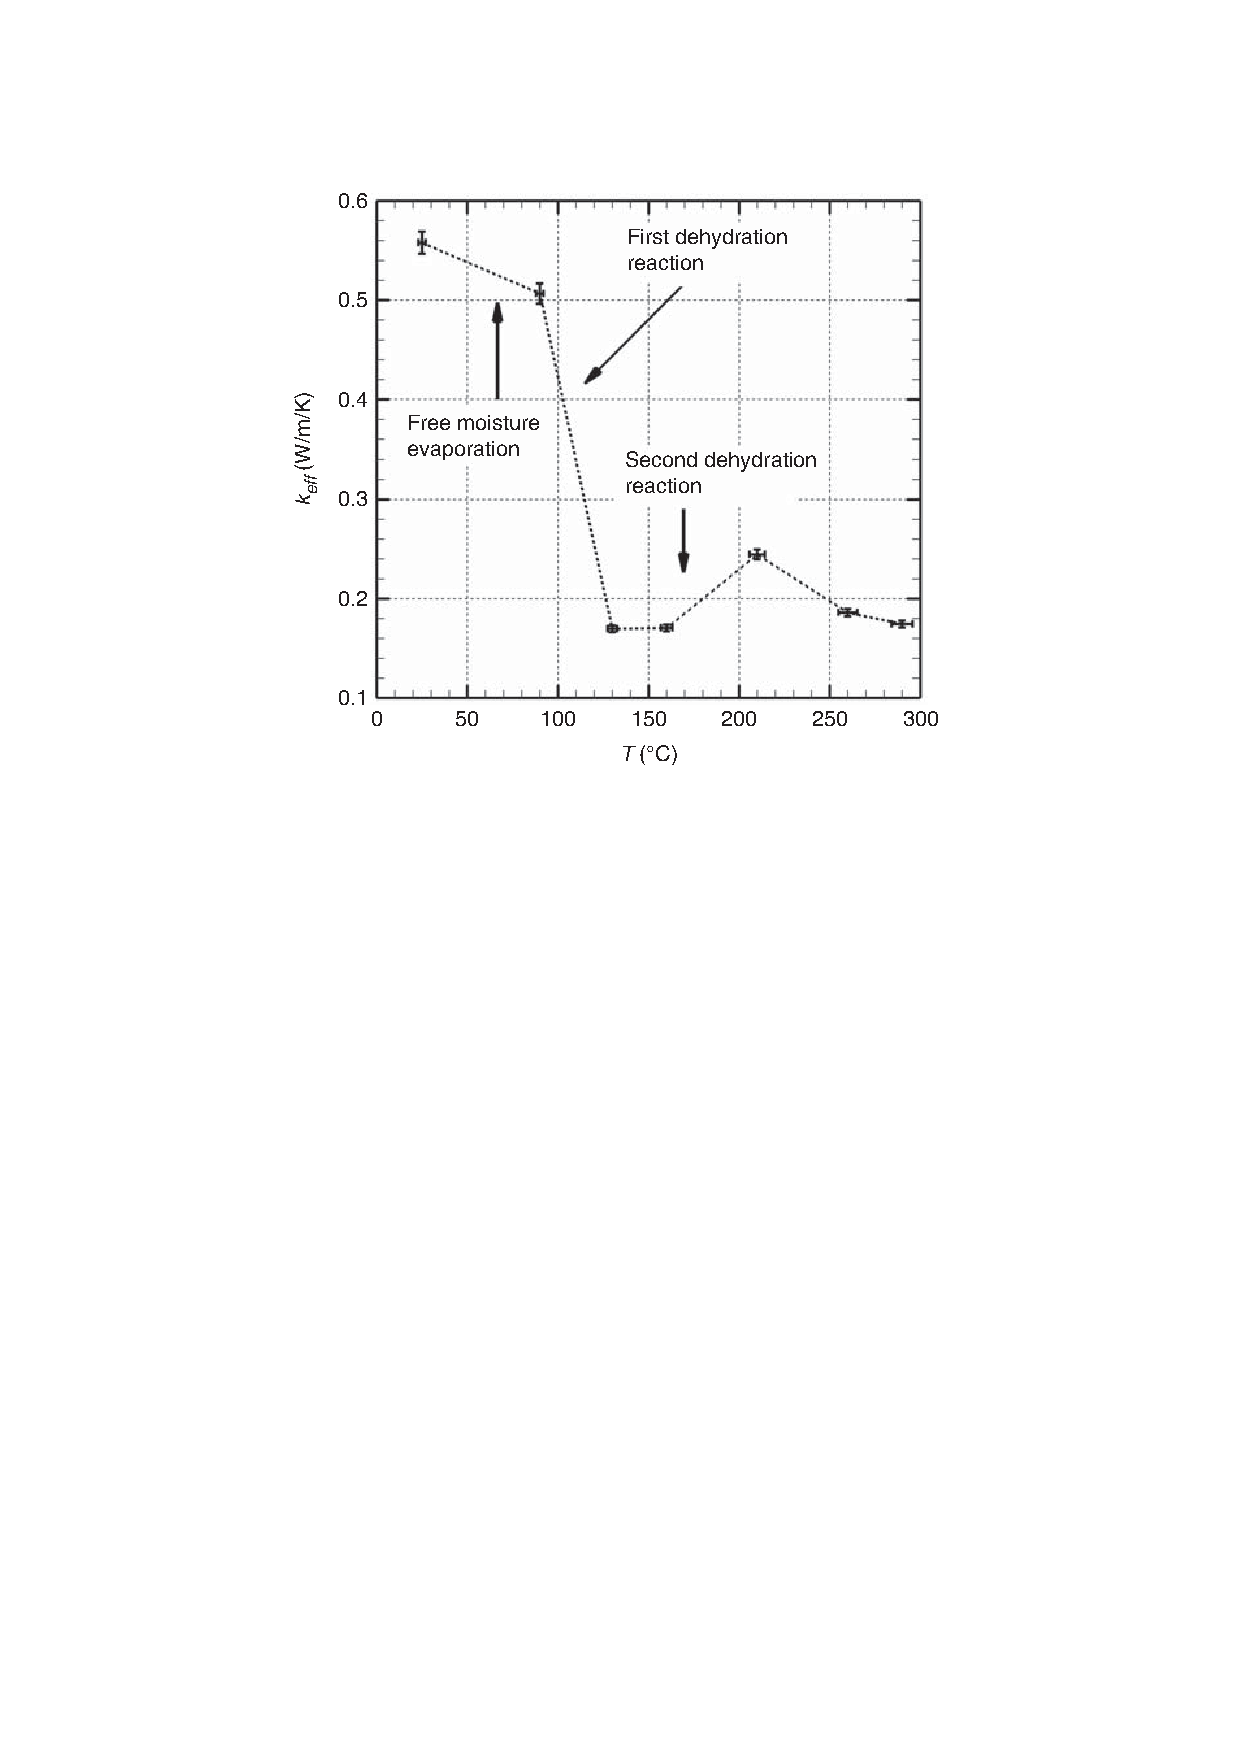
\includegraphics[width=6cm,height=5cm]{kontogeorgos_conductivity}		
		\caption{Thermal conductivity used by \citet{Kontogeorgos2011}}
		\label{fig:kontogeorgos_conductivity}
\end{figure}

This investigation concluded that due to the evaporation of free moisture content at about 100\degree C, the thermal conductivity decreases after the first dehydration point. Also, this research provided an experimental method to predict the energy absorbed by the gypsum plasterboard at dehydration point when exposed to elevated temperatures.

\section{Numerical Simulation}

\citet{Sultan1996} proposed a one-dimensional model to predict the heat transfer in non-load bearing and non-insulated LSF walls. Single row of steel studs spaced at 600 mm centres and 0.45 m thick were considered or the mathematical model. To reduce the complexity of the analysis the radiative heat transfer from the studs to the plaster-boards was ignored. Also the moisture movement and cracking of the plaster-boards were not considered. Time-Temperature profile from CAN/ULC-S 101-M89 was adopted for the model based on ASTM 119-16 (2016).

\begin{equation} \label{eq:sultan1996}
T_f = T_\infty + 750 [1-exp(-3.79553)\sqrt{\tau}] + 170.41\sqrt{\tau}
\end{equation}

Where
\begin{description}[itemsep=0pt,parsep=0pt]
	\item $T_f$ = Temperature of fire curve (source) (\degree K);
	\item $T_\infty$ = Temperature of Ambient side;
	\item $\tau$ = time, h.
\end{description}
The heat transfer through the wall from the fire side to the ambient side were governed by basic heat transfer equations of conduction, convection and radiation. The emissivity of the plasterboard was kept constant at 0.8 throughout the model. The convective heat transfer co-efficient was varied for different faces such as the fire exposed face, wall cavity and the unexposed face of the LSF wall as in \Cref{eq:hexp,eq:hcav,eq:huexp}.

\begin{equation}\label{eq:hexp}
h_{exp} = 0.95{(T_f - T_g)}^{0.33}
\end{equation}

\begin{equation}\label{eq:hcav}
h_{exp} = 0.95{(T_f - T_g)}^{0.33}
\end{equation}

\begin{equation}\label{eq:huexp}
h_{uexp} = 1.42{(T_g - T)}/L^{0.33}
\end{equation}

Where
\begin{description}[itemsep=0pt,parsep=0pt]
	\item $ h_{exp} $ = Convective heat transfer co-efficient (fire exposed side)
	\item $ h_{cav} $= Convective heat transfer co-efficient (cavity) 
	\item $ h_{u exp} $ = Convective heat transfer co-efficient (unexposed side) 
	\item $ T_f $ = Temperature of fire curve (source) (\degree K)
	\item $ T_g $ = Temperature of gypsum board (\degree K)
	\item $T$ = Temperature (\degree K)
	\item $L$ = Wall height (m)
	\item $d$ = Wall cavity depth (m)
\end{description}
Finite difference method was adopted to predict the temperature history across the wall and corresponding equations were proposed for different locations of the wall because of the varying boundary conditions. To validate the mathematical model, small-scale fire tests with specimen sizes of 1 $\times$ 1 m and 1 $\times$ 2 m were carried out with the same configuration adopted in the mathematical model. Thermocouples were used to measure the temperatures at different locations across the wall. The failure criteria for the fire test were in accordance with CAN/ULC-S 101-M89. The heat transfer mechanism in the fire test within the cavity was through natural and forced convection at different time of fire exposure and through radiation. This was not considered in the mathematical model. This research work resulted in clear insight of the heat transfer mechanisms across the LSF wall assembly. 

\citet{Keerthan2012a} conducted numerical studies of gypsum plasterboard panels. The thermal inputs such as thermal conductivity, specific heat, relative density and mass loss for the numerical analysis were derived through thermal properties test conducted on gypsum plasterboards. From the past research conducted on gypsum plasterboards by \citet{Mehaffey1994,Sultan1996} and other researchers, it is evident that, the plasterboard when exposed to fire above 800\degree C as per the ISO 834 standard fire curve will not stay intact. So apparent thermal conductivity values were used in the numerical models after 800\degree C. This is because, the plasterboard cracks after this temperature letting the hot gases to pass through, which cannot be predicted by the numerical model. The thermal conductivity, specific heat and relative density of plasterboards obtained from past research are shown in \Cref{fig:keerthan_pbprop} (a) to (c). Since there were discrepancies in the specific heat peak values, second dehydration point and relative density of plasterboards measured by past research works, experiments were carried out by \citet{Keerthan2012} using differential scanning calorimetry (DSC) and thermo gravimetric analysis (TGA). From the DSC heat flow data, specific heat was calculated as per ASTM E1269 (2011). The experimental results for specific heat, relative density and the proposed idealised thermal conductivity are shown in \Cref{fig:keerthan_measured} (a) to (c).

\begin{figure}[htbp]
	\centering
		\begin{tabular}{c}
			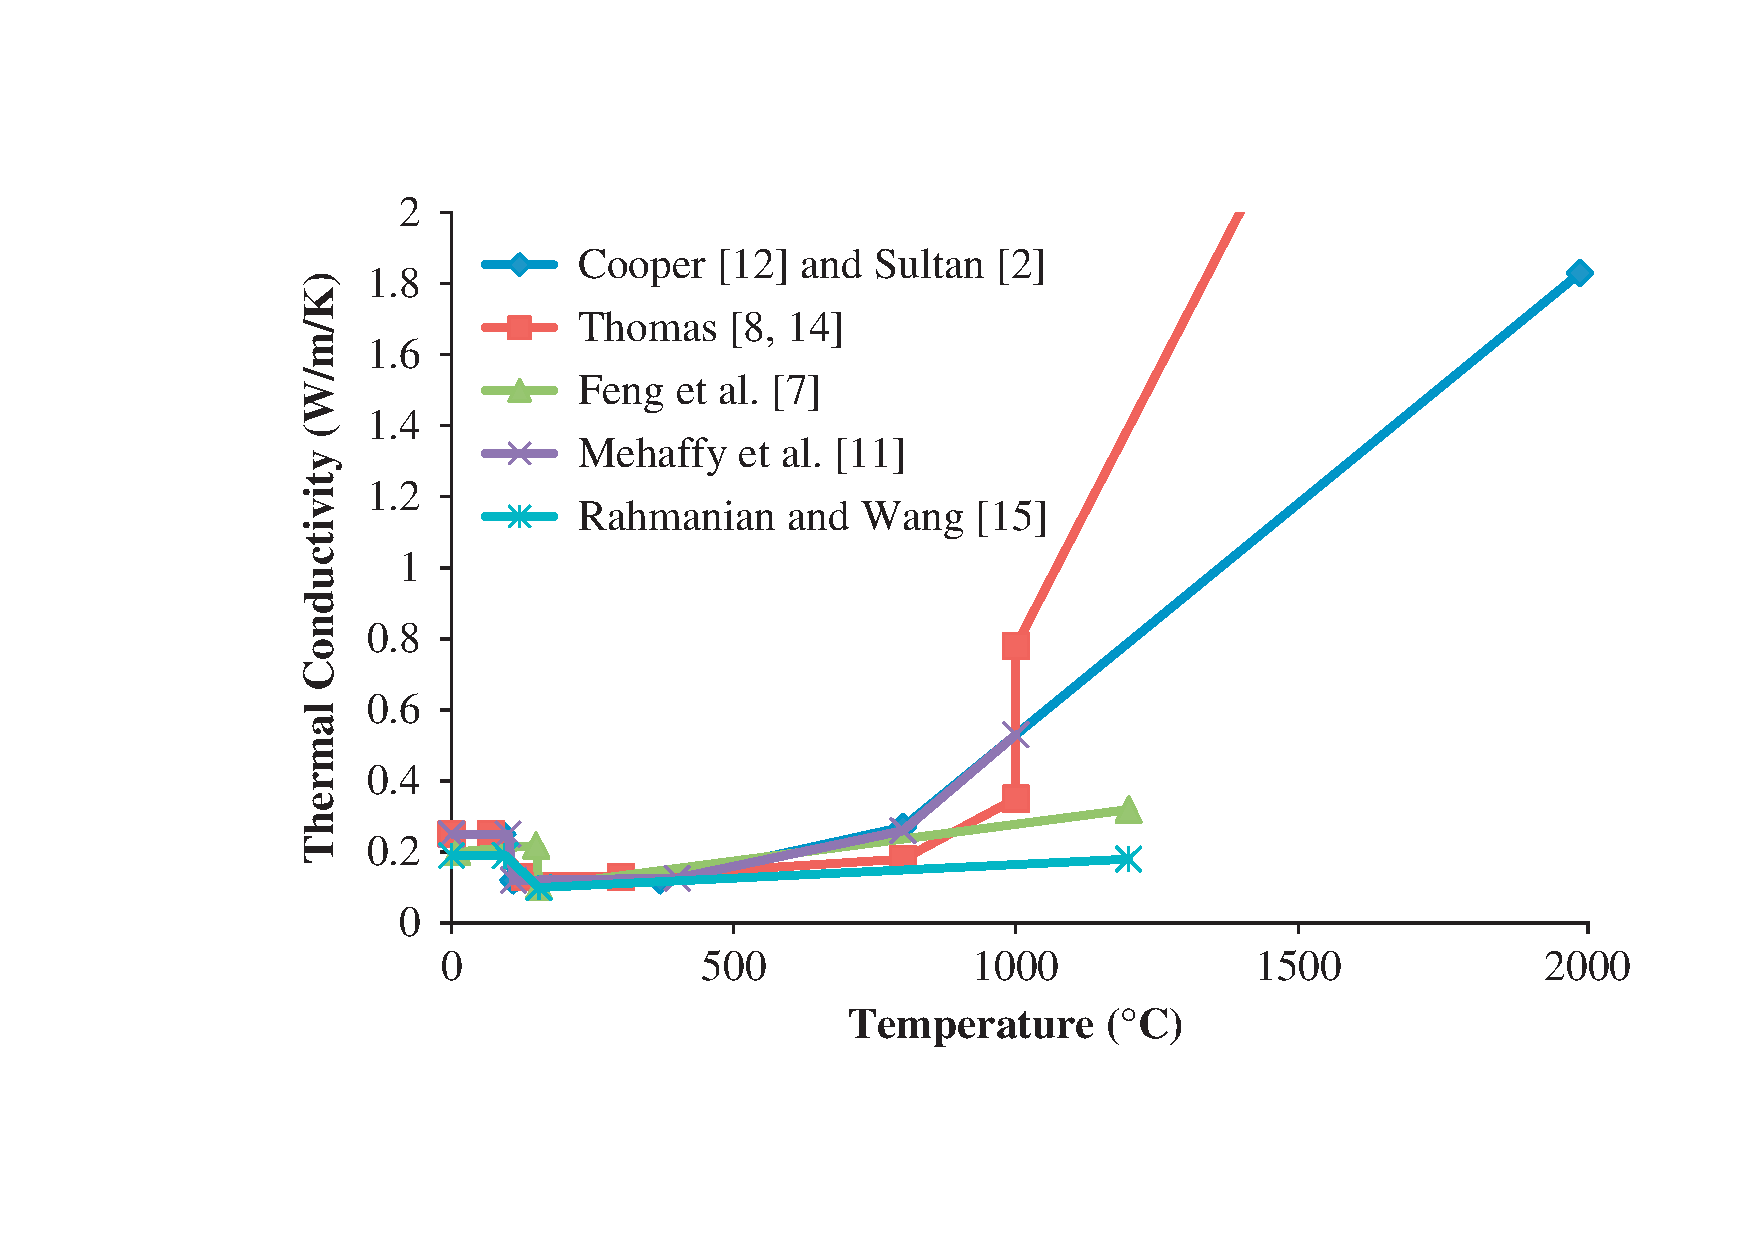
\includegraphics[width=8.5cm,height=6cm]{keerthan_conductivity.pdf} \\
			(a) \\
			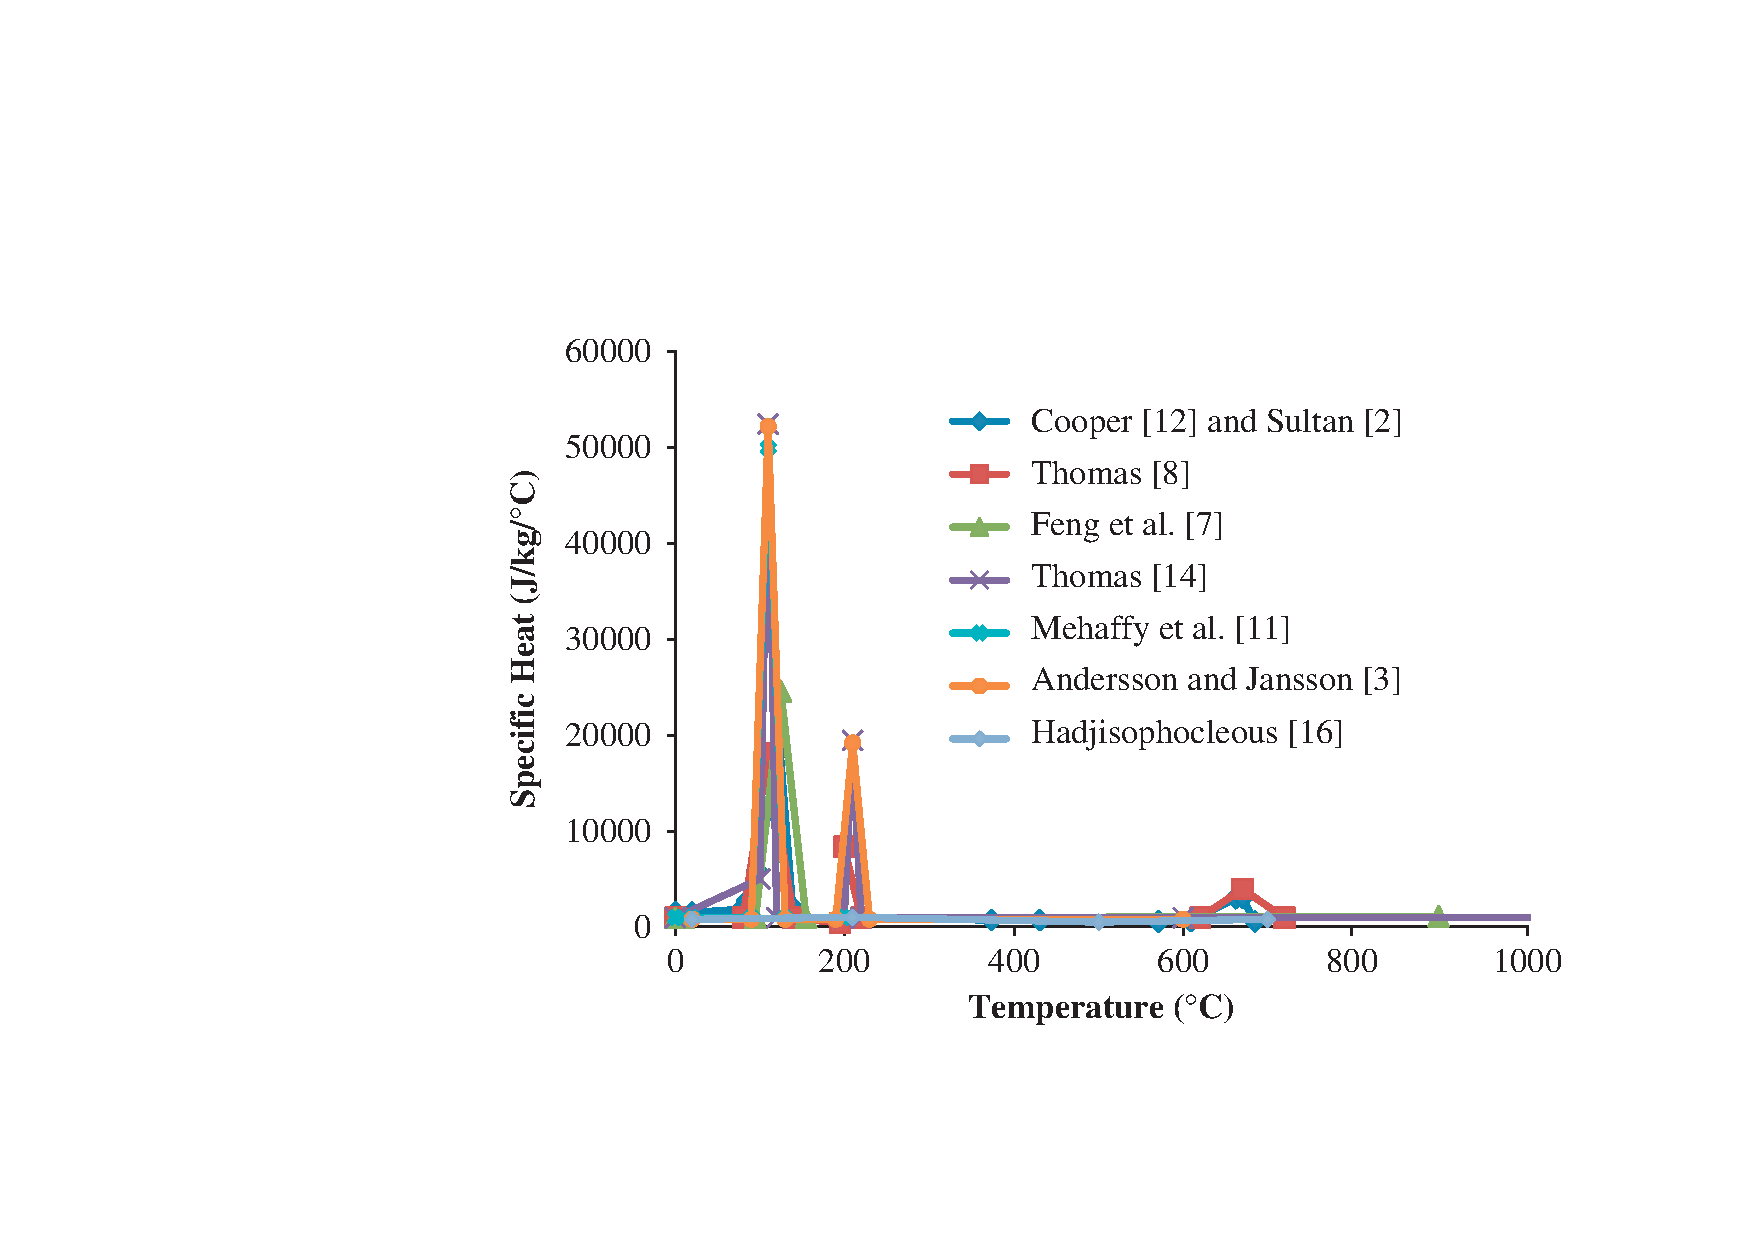
\includegraphics[width=8.5cm,height=5.5cm]{keerthan_cp.pdf} \\
			(b) \\ 
			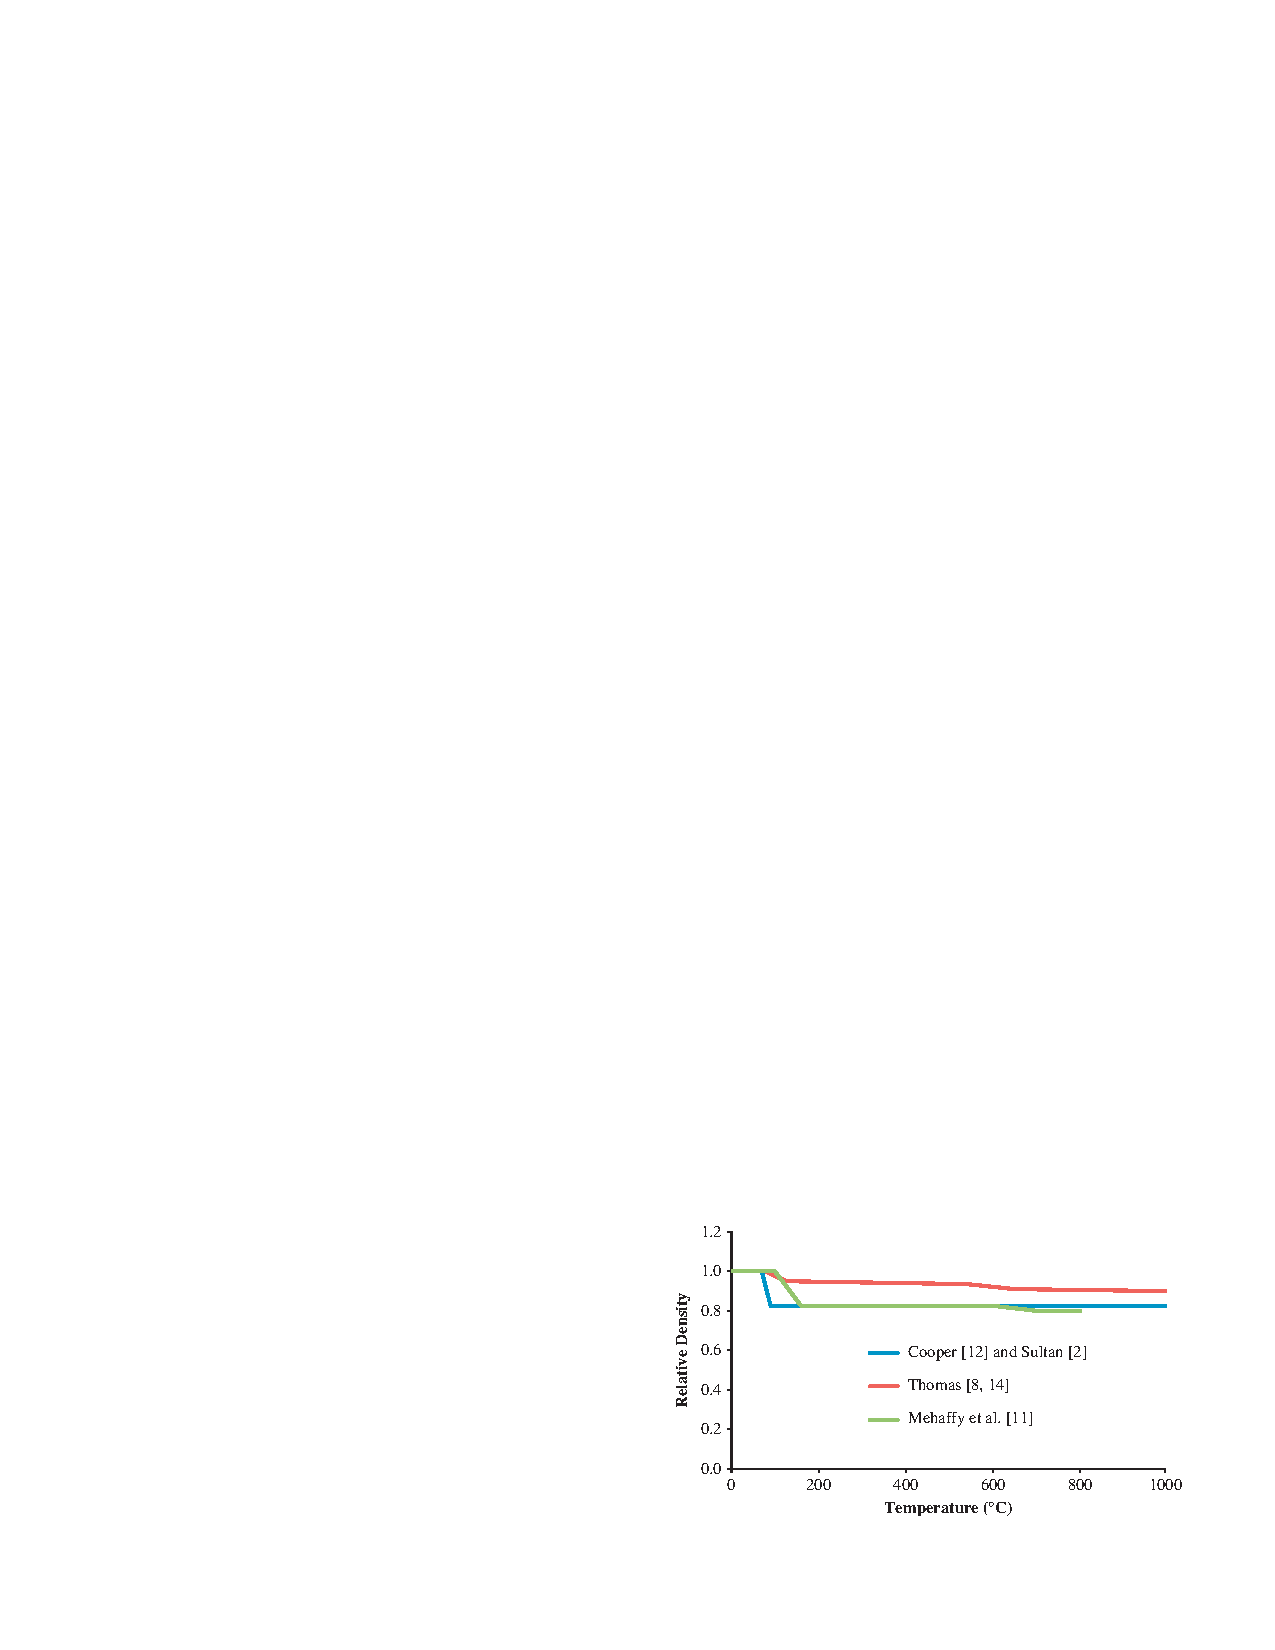
\includegraphics[width=8.5cm,height=5.5cm]{keerthan_density.pdf} \\
			(c) \\
		\end{tabular} 
		\caption{Thermal properties of plasterboard extracted from \Citet{Keerthan2012a}}
		\label{fig:keerthan_pbprop}
\end{figure}

\begin{figure}[htbp]
	\centering
		\begin{tabular}{c}
			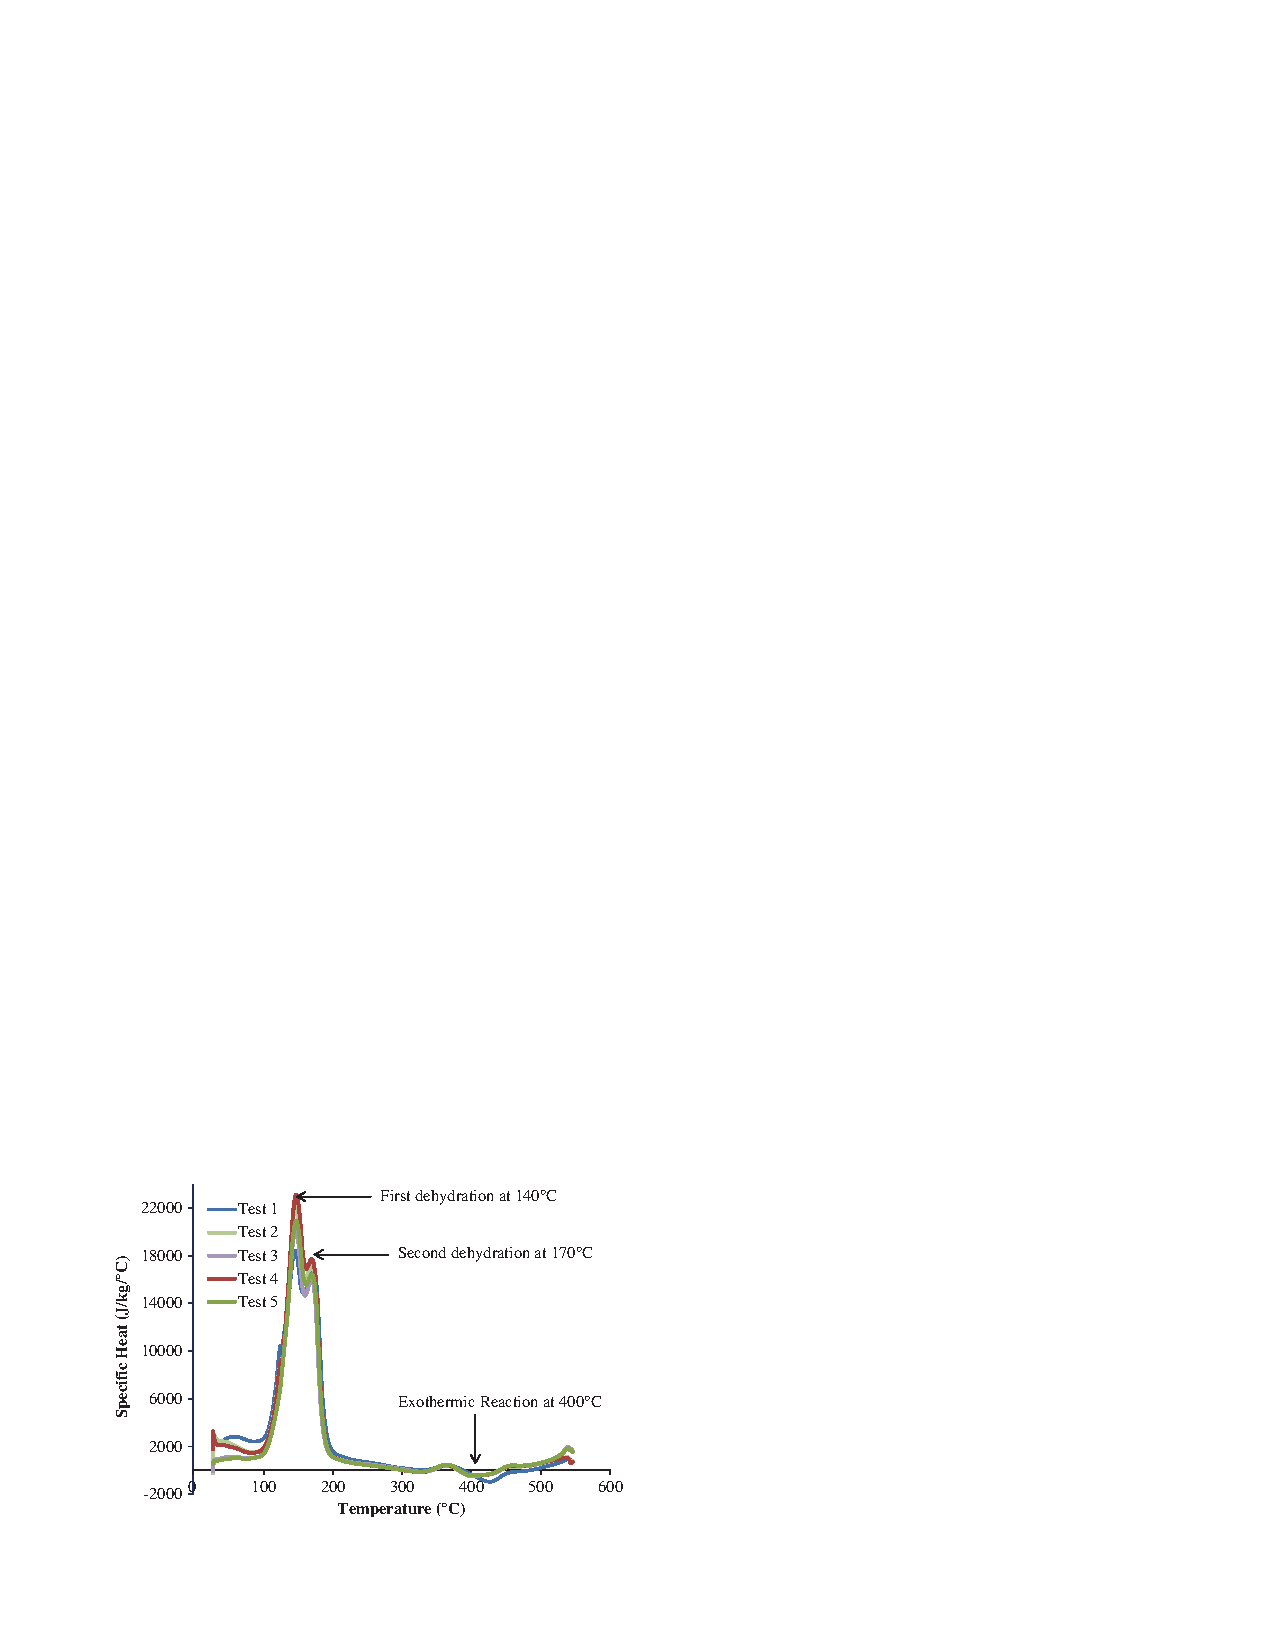
\includegraphics[width=8.5cm,height=6cm]{keerthan_cp_measured.pdf} \\
			(a) \\
			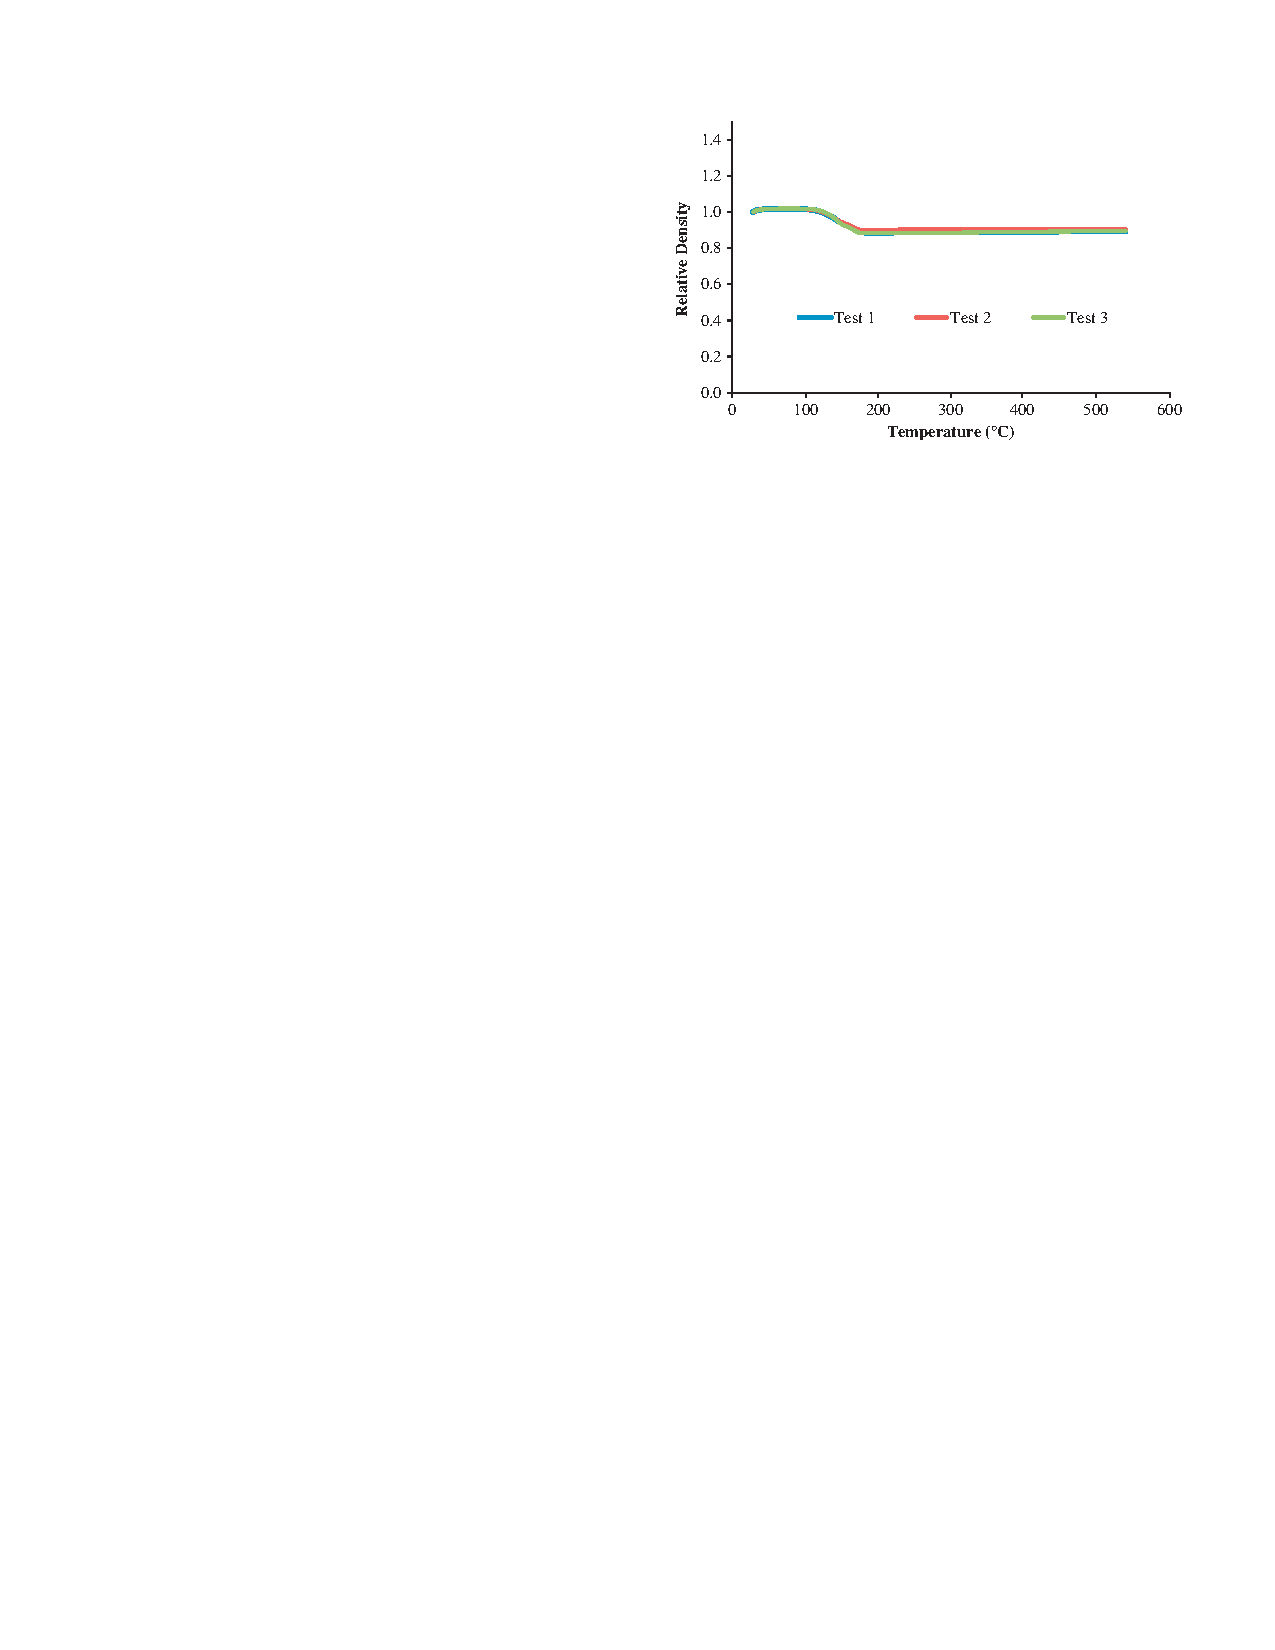
\includegraphics[width=8.5cm,height=6cm]{keerthan_density_measured.pdf} \\
			(b) \\ 
			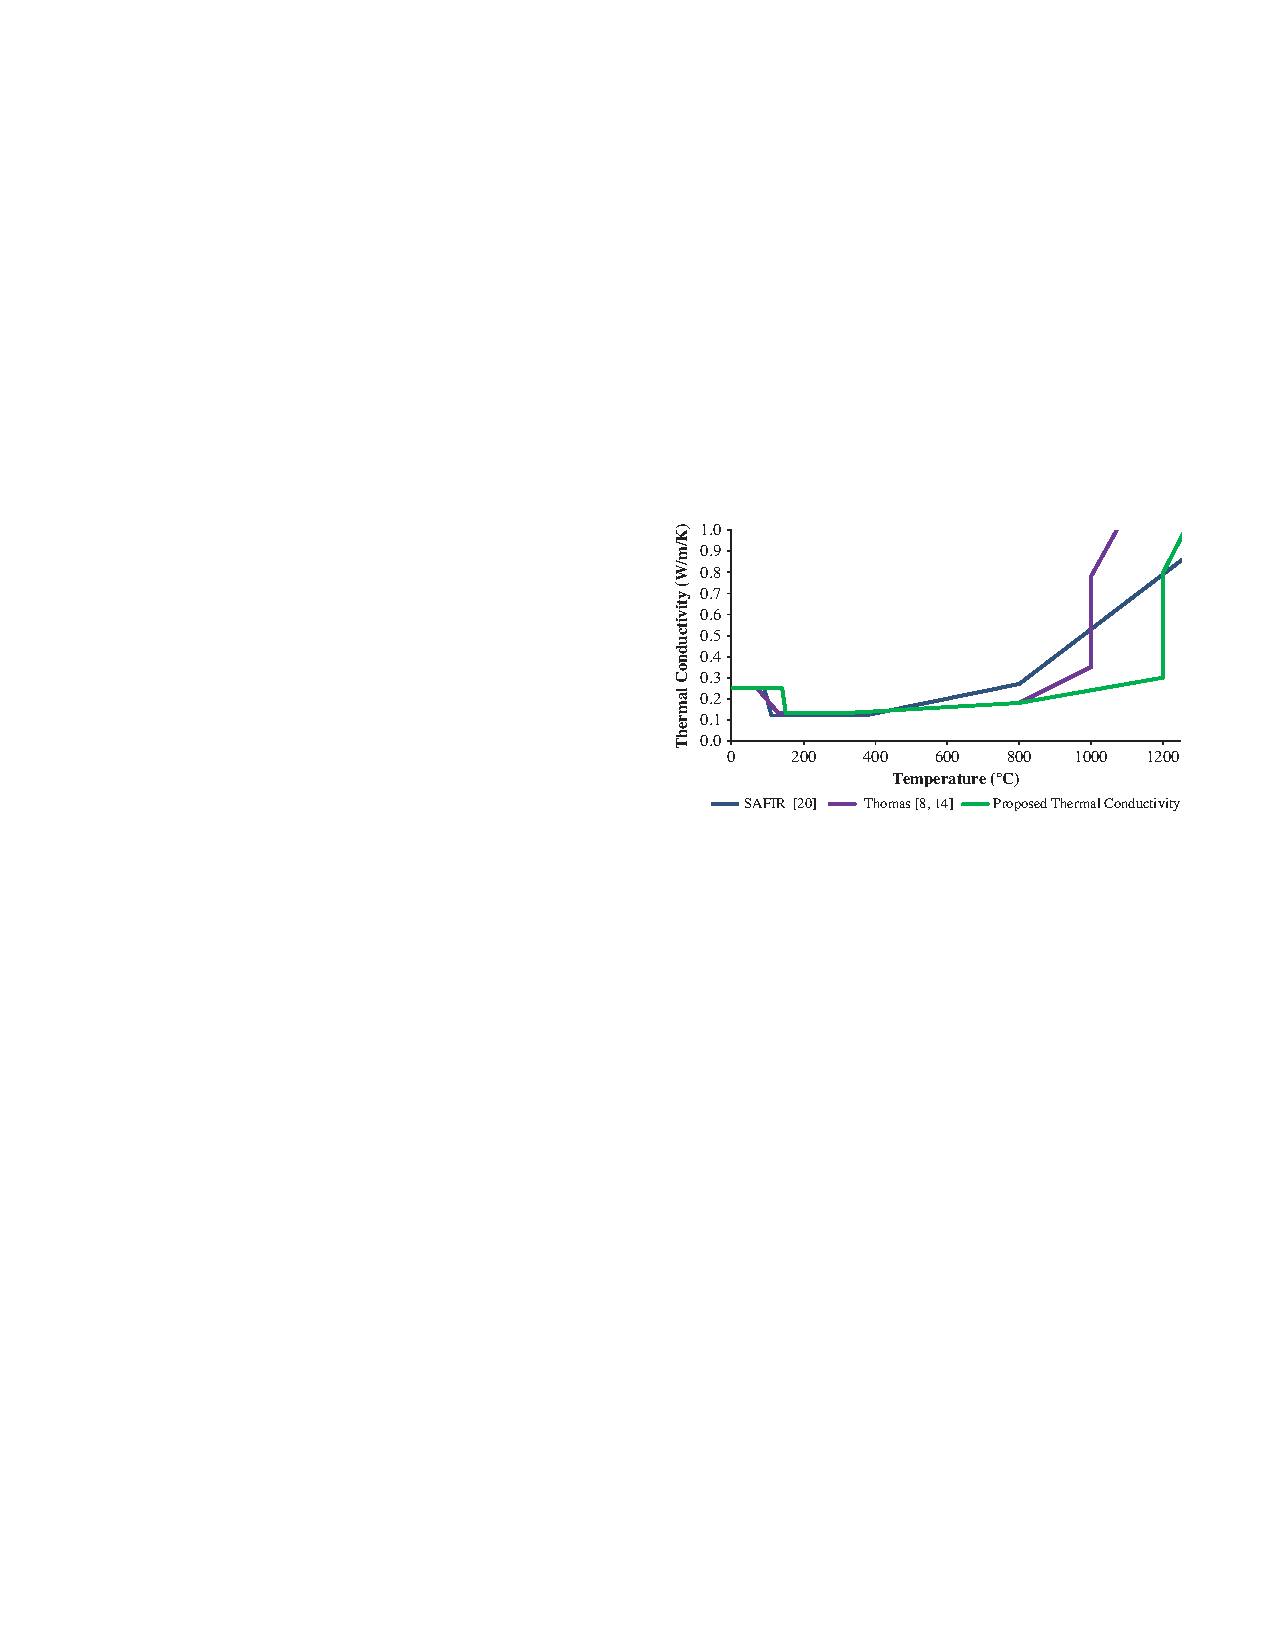
\includegraphics[width=8.5cm,height=5.5cm]{keerthan_conductivity_proposed.pdf} \\
			(c) \\
		\end{tabular} 
		\caption{Proposed thermal properties of plasterboard from \Citet{Keerthan2012a}}
			\label{fig:keerthan_measured}

	\end{figure}

These thermal properties were then used in the FE model developed in SAFIR and the results from the thermal analysis were compared with the small-scale fire tests conducted on plasterboards. It was concluded that, when the default thermal properties in SAFIR were used in the thermal analysis, there was not a good agreement between the FE model and the fire test. However, when the measured thermal properties were used in the thermal analysis, a good agreement was found between the small-scale fire test and FE model. The effect of moisture movement was not considered in the numerical analysis as the effect is not significant in temperatures above 120\degree C.

\Citet{Gunalan2013f} developed numerical models and validated them using the experimental results. Initially elastic buckling analysis was carried out by a finite strip analysis software called CUFSM. Various restraint conditions were used to study the elastic buckling behaviour. Then the elastic buckling load was expressed as load factor vs half-wave lengths and the different buckling modes were presented as shown in \Cref{fig:gunalan_buckling}.
\begin{figure}[htbp]
	\centering
		\begin{tabular}{c}
			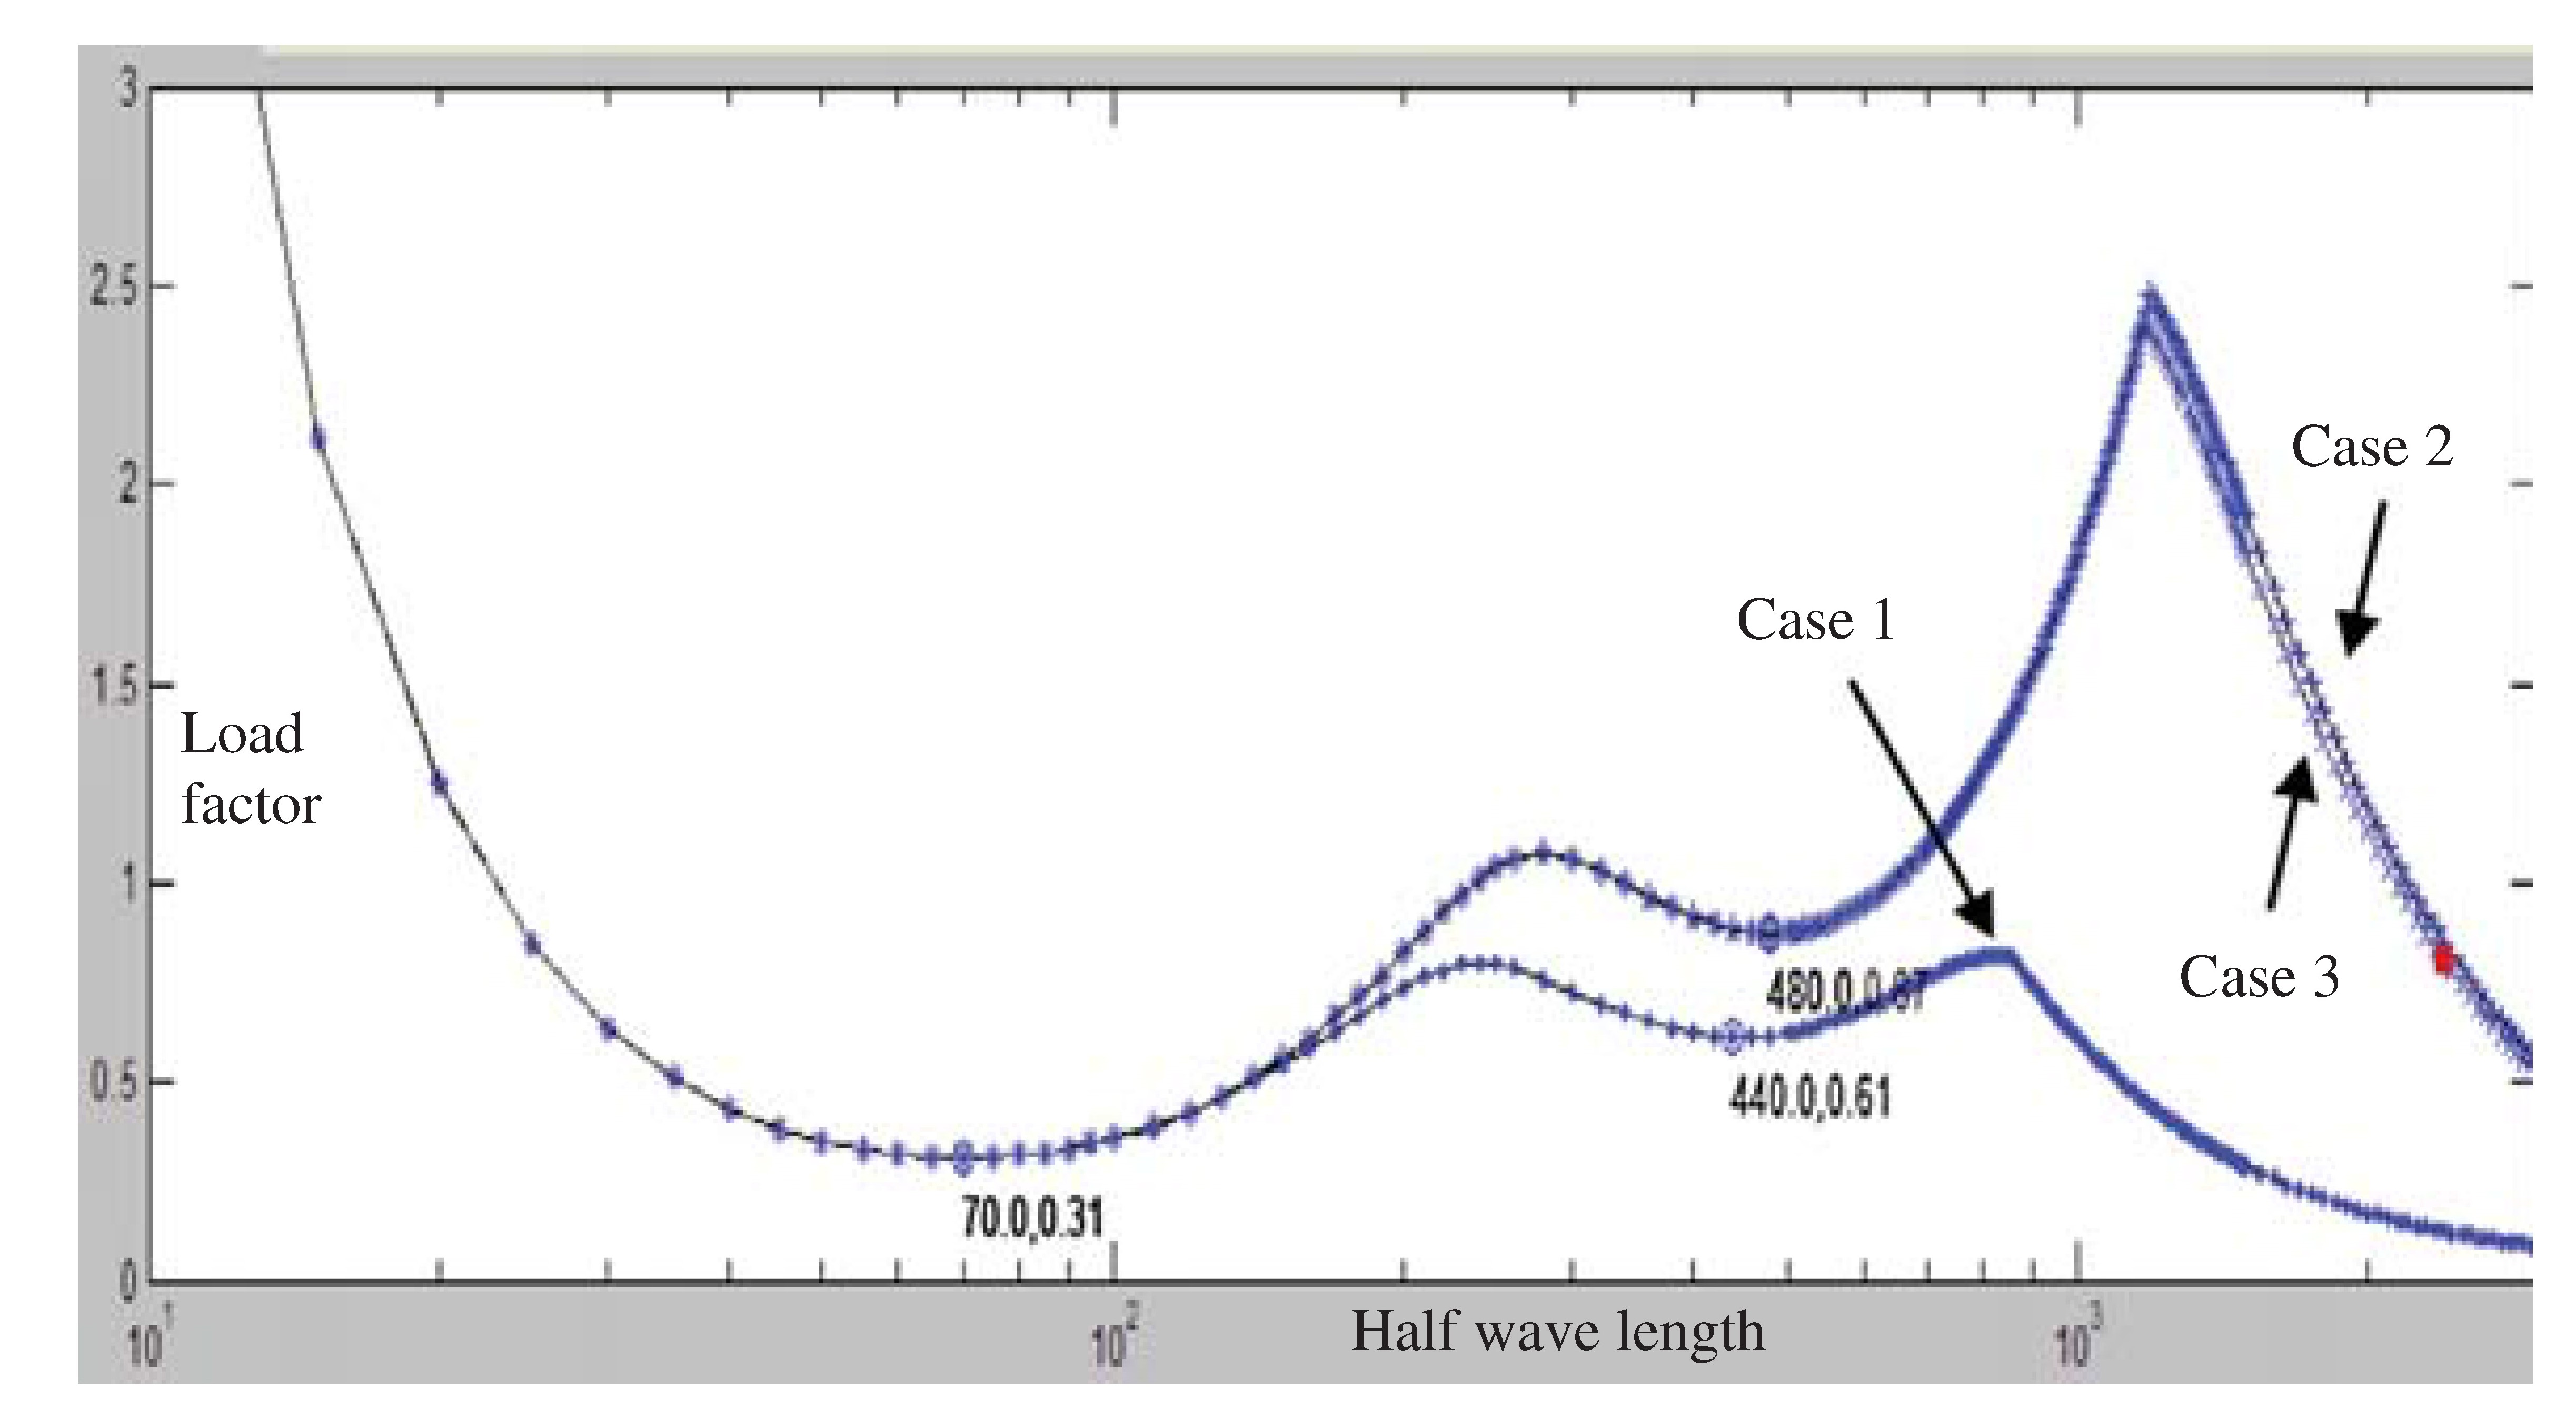
\includegraphics[width=8cm,height=4cm]{gunalan_halfwave} \\ 
			(a)	Load Factor vs Half-Wave Length\\ 
			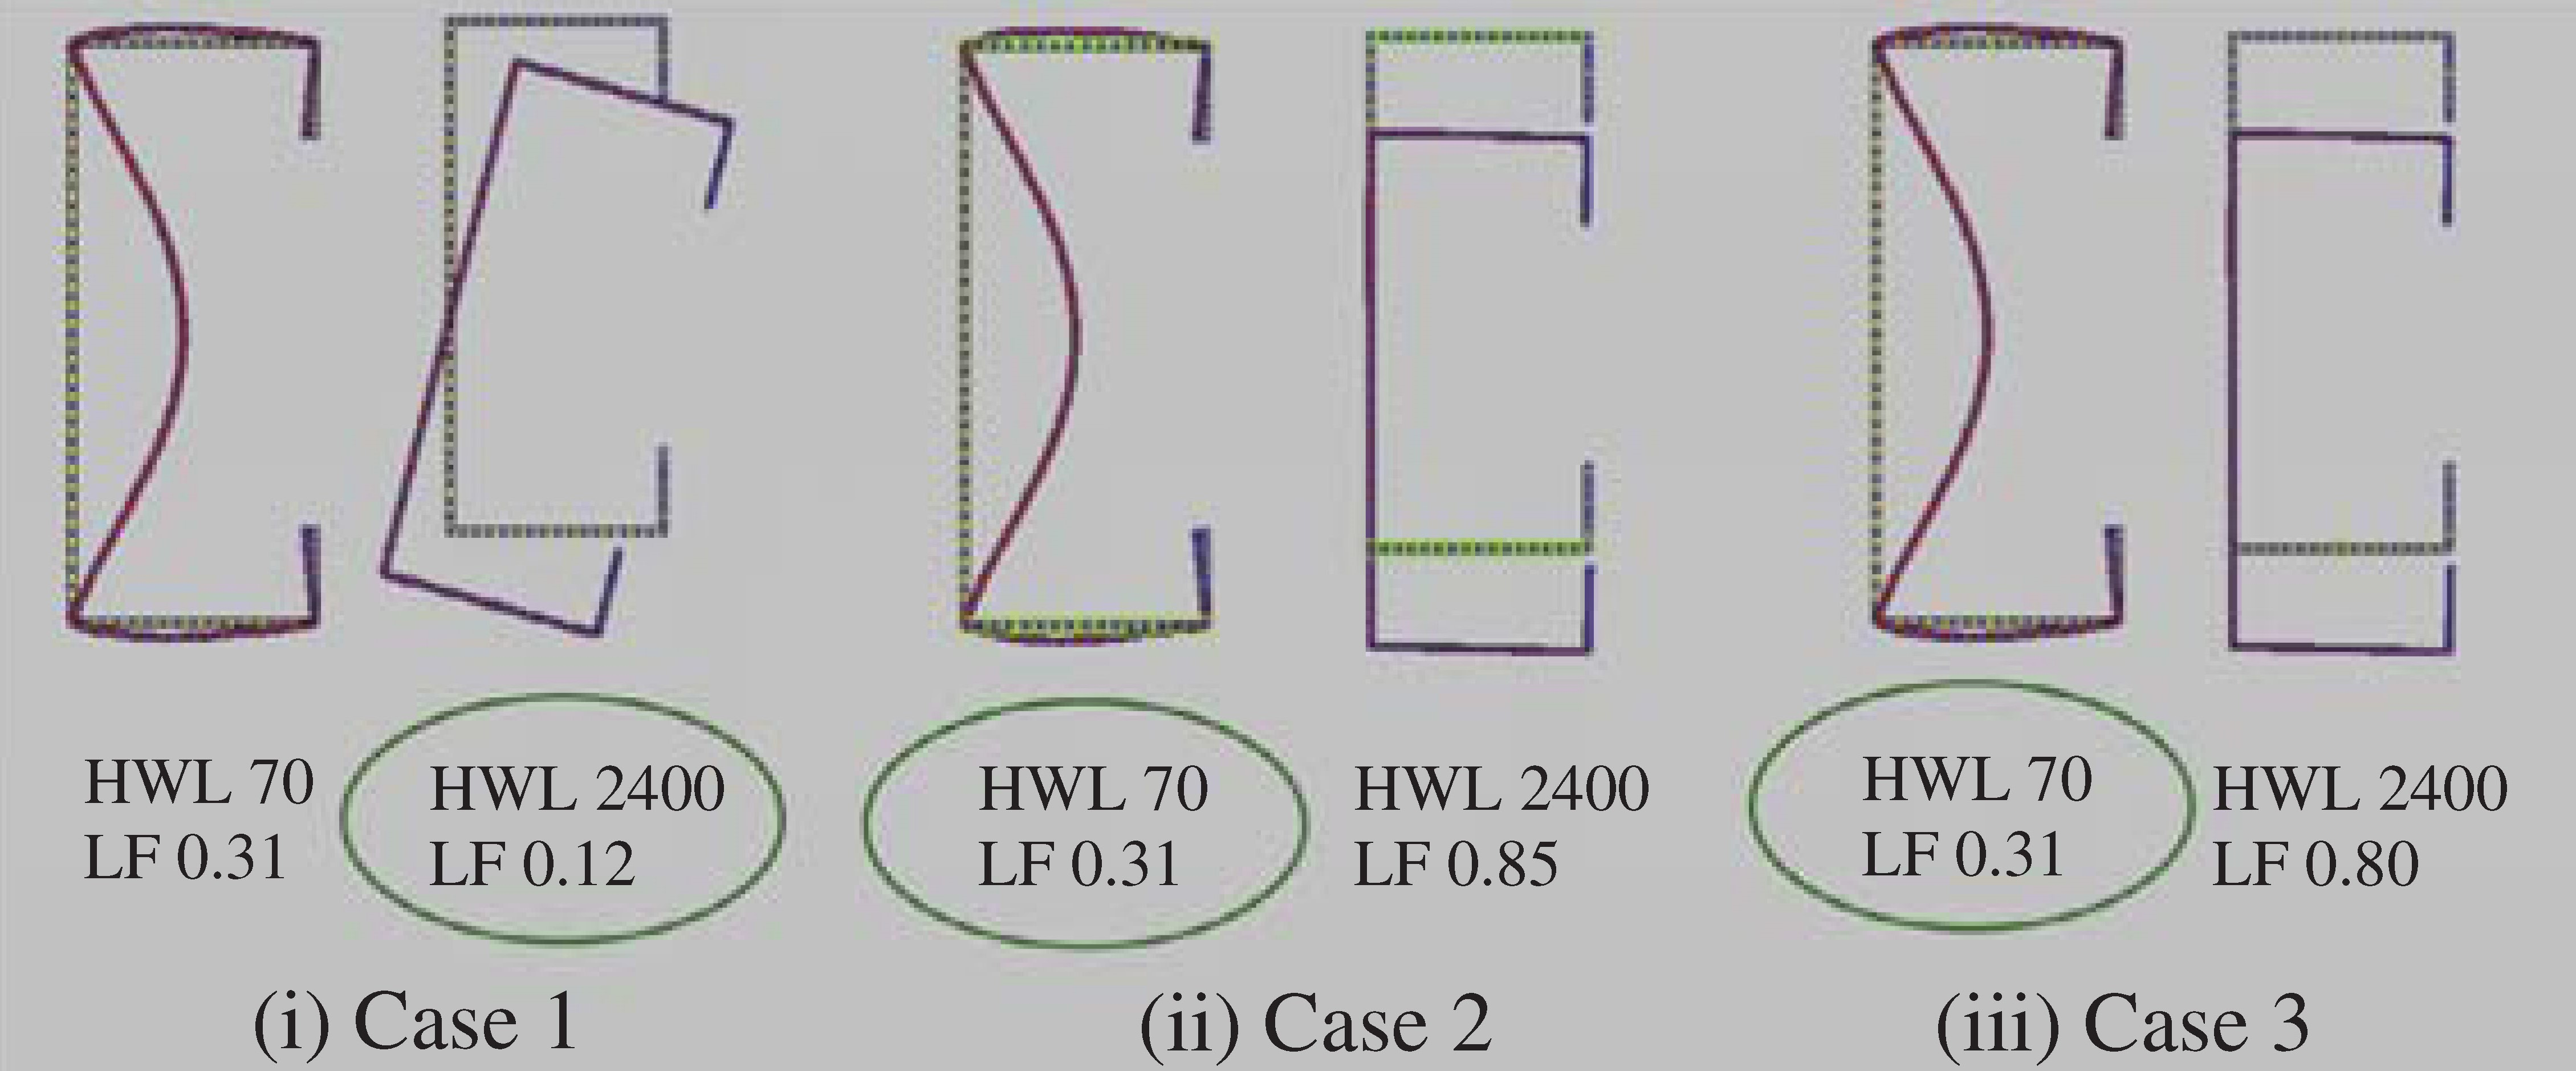
\includegraphics[width=8cm,height=4cm]{gunalan_buckling} \\ 
			(b)	Various Buckling Modes. \\ 
		\end{tabular} 
		\caption{Buckling analysis results from \citet{Gunalan2013f}}
		\label{fig:gunalan_buckling}
\end{figure}

Finite element modelling and analysis were carried out in ABAQUS for the conducted experiments. Mechanical properties such as Young’s modulus was determined by conducting tensile coupon tests. Since ABAQUS accepts true stress and logarithmic plastic strain, the engineering stress and strain from tensile coupon tests were converted to true stress and logarithmic plastic strain using the equations given as follows.

\begin{equation}
\sigma_{true} = \sigma_{eng}(1+\epsilon_{eng})
\end{equation}

\begin{equation}
\epsilon_{true}^{pl} = \ln(1+\epsilon_{eng})-\dfrac{\sigma_{true}}{E}
\end{equation}

The true stress and logarithmic plastic strain were then fed as input to the structural analysis. Thermal and structural boundary conditions were assumed in accordance with the experiments conducted and non-linear static structural analysis was carried out in ABAQUS. To simplify the thermal boundary conditions, it was assumed that the temperature distribution is linear on the webs from hot flange to cold flange and constant on the flanges. More complex effects such as thermal bowing and deterioration of the mechanical properties at elevated temperatures were studied from the numerical model and validated with the experimental results. New design rules based on AS/NZS 4600 and Eurocode 3 Part 1.3 were proposed by providing allowances for the thermal bowing effects, neutral axis shifts and magnification effects. These proposed design rules were then validated using the results from numerical analysis and were found to have good correlation. \citet{Gunalan2014a} further extended the study by investigating the effects of flexural torsional buckling of compression members at elevated temperatures. The mechanical properties of the steel sections after being exposed to fire were also investigated experimentally. Post-fire mechanical properties are needed to determine the residual strength of steel section after the fire. The residual strength is an important parameter to be considered by a structural engineer to assess the residual life of LSF wall systems. 

\citet{Nassif2014a} proposed a numerical model to predict the transient thermo-mechanical behaviour of LSF walls under fire. Full-scale 3 x 3 m wall panels were constructed with single row of studs and gypsum plasterboards were attached on both sides. Sequentially coupled analysis was carried out in ABAQUS and the results were compared with the experimental results. The thermal and mechanical properties for the numerical model were extracted from past literature and Eurocode. The numerical model was developed by considering the transient heat transfer behaviour of the LSF wall during fire. Conduction and convection on the fire exposed and unexposed faces of the wall were considered for the analysis. It was observed from the experiments and numerical models that the plasterboards provide considerable restraints to the steel studs against out of plane deflection. The proposed numerical model predicted the temperature of the steel studs and plasterboard to certain accuracy. However, during the plasterboard fall-off, the temperatures increase rapidly during the experiments and the model could not predict this uncertain behaviour. 

\citet{Chen2014} developed a numerical model to predict the thermal and mechanical response of cold formed steel (CFS) under fire. With the help of measured material properties, a one dimensional thermal response model was formulated to predict the heat transfer mechanism across the width in LSF walls under fire. Gauss-Seidel method was used to solve the governing equations expressed in the form of finite-differential equations. A thermomechanical response model was also developed to predict the axial and lateral deformations in the CFS wall system. Following assumptions were made to simplify the model.
\begin{itemize}
	\item Heat transfer was assumed to happen in the horizontal direction across the width of the wall only. 
	\item Variation in heat transfer due to the steel studs was ignored.
	\item Apparent thermal properties for specific heat was assumed to incorporate the effects of moisture transfer and plasterboard cracking.
	\item Plasterboard cracking was assumed to happen when the temperature increases beyond the threshold limit.
	\item Despite the variation in temperatures along the height of the wall due to air movement, this effect was neglected for the numerical model.
	\item As the cross-section area of studs are comparatively less than the cavity, conduction through studs were assumed to be less significant and the corresponding effects were also neglected.
	\item Different failure mode criteria were assumed to predict the failure time for CFS wall assemblies in the thermomechanical model.    
\end{itemize}
Despite the above mentioned simplifications, the numerical model was able to predict the experimental time-temperature and lateral deflection curves with reasonable accuracy. 

\citet{BatistaAbreu2015} proposed advanced numerical modelling of the LSF wall panels. Conventionally, the studs were modelled individually for thermal and structural analysis. However, the plasterboards were also modelled along with the studs and the opening of the joints were assumed, so that, the numerical model simulated the experimental behaviour to greater precision. Sequentially coupled thermal and structural analyses were used in the numerical model developed in ABAQUS. The stiffness of fasteners sheathing system was also investigate numerically as a part of this study. Design equations for normal and fire rated gypsum boards were also proposed. It was concluded that the Finite Strip Method and Finite Element Analysis are the most efficient methods of structural analysis for cold-formed steel sections.  

\citet{Cheng2015} developed a model to perform buckling analysis of the lipped channel cold-formed steel sections at elevated temperatures. Their investigation was conducted by performing heat transfer analysis initially, followed by pre-buckling and post-buckling analysis. Finite element analysis was used for the heat transfer problem. Bernoulli’s beam theory was used for the pre-buckling analysis by considering the strain effects due to variation in mechanical properties at elevated temperature. Finite strip analysis and classical Fourier solutions were used for the buckling analysis. It was observed that the buckling behaviour of cold-formed steel sections varied under non-uniform temperature exposure when compared with uniform temperature exposure. It was concluded that the higher temperature regions (hot-flange) had lower pre-buckling stresses whereas the lower temperature regions (cold-flange) had higher pre-buckling stresses. Also, the fire design formula for beams under uniform temperature exposure will not be suitable for sections with non-uniform temperature distribution.

The local buckling effects of cold-formed steel compression members were investigated in detail by \citet{Gunalan2015}. Using 91 local buckling tests, experimental results were compared with the numerical predictions from ABAQUS for validation purposes. The cold-formed sections for the local buckling tests were selected using ABAQUS and CUFSM on condition that local buckling occurred at ambient conditions. For elevated temperatures, reduced mechanical properties were used in ABAQUS and CUFSM to find the elastic buckling loads. Shell S4 elements were used in the finite element model. Geometric imperfections proposed by Schafer et al. (2010) for lipped channel sections and Camotim et al. (2006) for plain channel sections were used. Steel grades of G250, G450 and G550 were used in this research. The ambient temperature mechanical properties of G250 and G550 steels were used based on Ranawaka and Mahendran (2009a) while for G450 steel, they were obtained from Kankanamge and Mahendran (2011). It was concluded that, the design rules at ambient temperature can be used to predict the buckling behaviour at uniform elevated temperature by considering reduced mechanical properties. The effective area method at ambient temperatures as per Eurocode 3 Part 1.2 resulted in over-conservative results at elevated temperatures also. It was also proposed that at elevated temperatures the current design rules can be improvised by incorporating the effects of non-linear stress-strain relationships.

\citet{Kesawan2015a} developed a 2D numerical heat transfer model using SAFIR. The aim of this research was to develop a numerical model for validating the fire tests conducted using HFC steel studs by \citet{Kesawan2015}. A 2D model replicating the fire test was created in SAFIR and the corresponding thermal properties of the materials were keyed in to carry out heat transfer analysis. Heat transfer along the height of the wall was neglected for computational efficiency. GiD, a general purpose pre and post processor software, was used to create models, assign meshes and view the results after analysis. Overall mesh dimension of 8 mm was incorporated into the model based on the research from \citet{Keerthan2012}. Moisture transfer and plasterboard cracking effects were ignored in the thermal analysis considering their insignificant contribution to the FRL. Localised temperature rise in studs due to plasterborard fall-off was also ignored due to the complexity in modelling the same. From the thermal analysis results, it was found that the time-temperature curves of the plasterboards and studs agreed reasonably well with the experimental results in non-cavity insulated HFC walls, while there were minor disagreement with cavity insulated HFC walls. 

A detailed parametric study by considering the variation in stud depth and flange width was also carried out in SAFIR as part of this research. The parametric thermal analysis results shows that the variation in stud time-temperature curves with increase in cavity depth/ stud width did not significantly change. This indicates that, the heat transfer through conduction in stud remains unchanged with increase in cavity depth. However, the time-temperature curves comparison of plasterboards were not presented. It was stated that the same time temperature profile of studs can be used to determine the FRL irrespective to the cavity depth which is debatable. The effect of stud thickness was also investigated. Stud thicknesses from 0.6 mm to 3 mm were taken for the parametric study. The thermal analysis results showed that for thicker stud section the hot flange temperatures were lower, while the cold flange temperatures were higher in comparison with the thinner sections. The effect of stud thickness was found to affect the temperature profiles in cavity insulated walls significantly. Increase in stud spacing was also investigated and was found to have no significant effects on the time-temperature curve. The thermal performance of different wall configurations was also investigated. Later \citet{Kesawan2016} extended the study to develop fire design rules for hollow flange channel sections subjected to non-uniform temperatures under fire. The improved fire design equations were based on AS/NZS 4600 and Eurocode 3. Direct strength method (DSM) based equation was also proposed and verified based on the experimental and numerical work conducted earlier. The load ratio versus FRL curves derived earlier by \citet{Kesawan2015a} were now obtained using the AS/NZS 4600 and Eurocode 3 design equations. The modified design equations used for this study were based on \citet{Gunalan2013a} along with those from AS/NZS 4600.  

The section moment capacities at stud mid-height and supports were computed by the equations \Cref{eq:M_mid-height,eq:M_support} and are given below.
\begin{equation}\label{eq:M_mid-height}
M_{x,eff} = \dfrac{\bar{f}_{yt}\bar{I}_{eff},t}{y_{max}}
\end{equation}
\begin{equation}\label{eq:M_support}
M_{x,eff} = \dfrac{f_{yt,hf}\bar{I}_{eff},t}{y_{max}}
\end{equation}
The thermal bowing effects were computed based on the modified equation by \citet{Baleshan2016a} as they were found to be less complex and is given in \Cref{eq:bal_e-delta}.
\begin{equation}\label{eq:bal_e-delta}
e\Delta_T = \dfrac{(\alpha_{OHF}OHF-\alpha_{OCF}OCF)L^2}{8d}
\end{equation}
The ratio between end moments $\psi$, was taken as -1 at stud mid-height despite the fact that the value of $\psi$ is greater than -1 and also the actual values. Comparison was made against conventional LCS section with HFC section of similar web depth to understand these effects. The following modifications were made to the design equations. At the stud supports the P-$\Delta$ effects were neglected. \citet{Baleshan2016a} thermal bowing equations were used and the actual value of $\psi$ for the bending capacity calculations were computed. Improvements were made to the Eurocode 3 Part 1.3 based equations apart from the AS/NZS 4600 based design equations. Design capacities were also predicted based on Direct Strength Method (DSM) as well. It was found that, the proposed design modifications to the existing equations were able to predict the structural capacities of HFC section under fire to a reasonable accuracy. Comparisons were also made against the FE model predictions from ABAQUS by \citet{Kesawan2016a} to investigate the suitability of these modified design equations. 

Later, \citet{Kesawan2018} reviewed the parameters influencing the fire performance of LSF walls. Important parameters such as plasterboard fall-off, wall configuration, geometric profile of the studs, thermal and mechanical properties of various components at elevated temperatures were discussed in detail based on previously conducted experimental and numerical studies. The effect of plasterboard joints was also discussed in detail. As the fire performance of cavity insulated walls is significantly less in comparison with non-cavity insulated walls, four new LSF wall configurations by externally insulating the walls were proposed in this research. The option of providing plasterboard strips as back blocking to the studs was also proposed to improve the fire performance. However, only limited experimental studies were conducted for the proposed configurations and detailed FE analysis has to be conducted to support the above claims. It was also proposed that the usage of large fasteners would increase the contact area of screws on plasterboards thereby reducing the plasterboard fall-off during fire. But it is difficult to quantify these effects as substantial experimental and numerical investigation has not been carried out on these effects. The temperature gradient within the studs was found to have significant influence on the FRL, as the difference in stud hot and cold flanges can result in premature structural failure. Different geometric shaped studs was also proposed and the influence of temperature distribution amongst them was also compared with the help of FE analysis. However, these need to be validated with the help of experimental studies as well.

\citet{Ariyanayagam2016} investigated the detrimental effects of the plasterboard joints on the fire performance of LSF walls. 150 mm wide plasterboard back blocking was used in the LSF wall panels and standard fire tests were conducted to investigate the detrimental effects of plasterboard joints under fire. Two full scale fire tests at 0.2 load ratio were conducted. The first LSF wall had plasterboard joints between the studs and the second LSF wall had plasterboard joints in between the studs with the help of back blocking. The test wall panel was 2.1 x 2.4 m with four studs spaced at 600 mm centres. No noggings were used in the LSF wall panel. Fire test results showed that, the middle studs (2 \& 3) recorded higher hot flange temperatures in the wall panel, where plasterboard joints were present on the studs when compared to the wall panel with plasterboard joints on back blocking. The failure time of the wall with back blocking plasterboard joint was 74 minutes whereas the conventional specimen lasted only 58 minutes. Numerical investigations were carried out in two steps. Initially, steady state analysis with temperature inputs from the experiments at different time periods were carried out. S4R elements were used for the studs with a mesh size of 4 mm and rigid body with R3D4 elements were used to apply the load to the studs. The studs used in this investigation were made of 1.15 mm G550 steel. The studs were maintained at different temperatures in correspondence with the experiments. The axial compression load was applied and Riks analysis was carried out to achieve the failure of the stud. It was concluded that by providing back blocking to the plasterboard joint in load bearing LSF walls, the FRL of the wall was increased by up to 25\%. However, the plasterboard joints did not have any effect on the non-load bearing LSF walls which is generally governed by insulation failure.

\citet{Dias2018} developed a thermal finite element model in ABAQUS to investigate the thermal behaviour of web-stiffened stud LSF walls in fire. Thermal and structural modelling were conducted for the tested LSF wall configurations using small-scale fire tests. The modelling techniques were adopted from \citet{Rusthi2017}. Web stiffened studs were found to yield better compression capacity under ambient condition in comparison with the conventional lipped channel studs. However, the capacity of the same was not found to provide better results under fire when non dimensional parameter FRL was considered. The susceptibility of non-load bearing LSF walls failing under structural integrity criteria was also discussed based on the conducted FE analysis. However, experimental results were not available to validate this claim. 

\section{Computational Fluid Dynamics (CFD)}

Computational fluid dynamics is a branch of fluid mechanics, in which the numerical problems with respect to fluid flows are solved by numerical analysis and algorithms. Problems related to wind flow and heat transfer are also solved by CFD. The discretization of the problem is undertaken using various methods in CFD such as Finite Element Method, Finite Volume Method, Finite Difference Method, Spectral element method and Boundary element method. Any ideal CFD model will be a dependent of the Navier-Strokes equation.  

To address a heat transfer problem for a model based on Finite Element Method, coupled temperature displacement method is used. In this, the conduction, convection and radiation coefficients, used as input to the analysis and the heat transfer problem is solved. Whereas, in a CFD model these parameters can be input as a 3- dimensional entity to arrive at precise results. ABAQUS CFD / ANSYS Fluent package is proposed for the analysis of the advanced heat transfer problems to be taken up in this research as part of the numerical validation process.

\citet{Horvat2009} proposed a semi-analytical treatment of wall heat transfer coupled to numerical simulation model of fire. The objective of this study is to develop a computational technique to predict the heat flow through walls by simulating mass and momentum across the wall when exposed to fire. A numerical model for heat transfer was developed in CFX. 1.2 m long x 0.8 m wide x 0.8 m high room size which is one third of the ISO room size was considered in the numerical model as shown in \Cref{fig:horvat_model}. A 25 mm thick insulation was considered for the walls and ceiling in the model.
\begin{figure}[htbp]
	\centering
		\begin{tabular}{cc}
			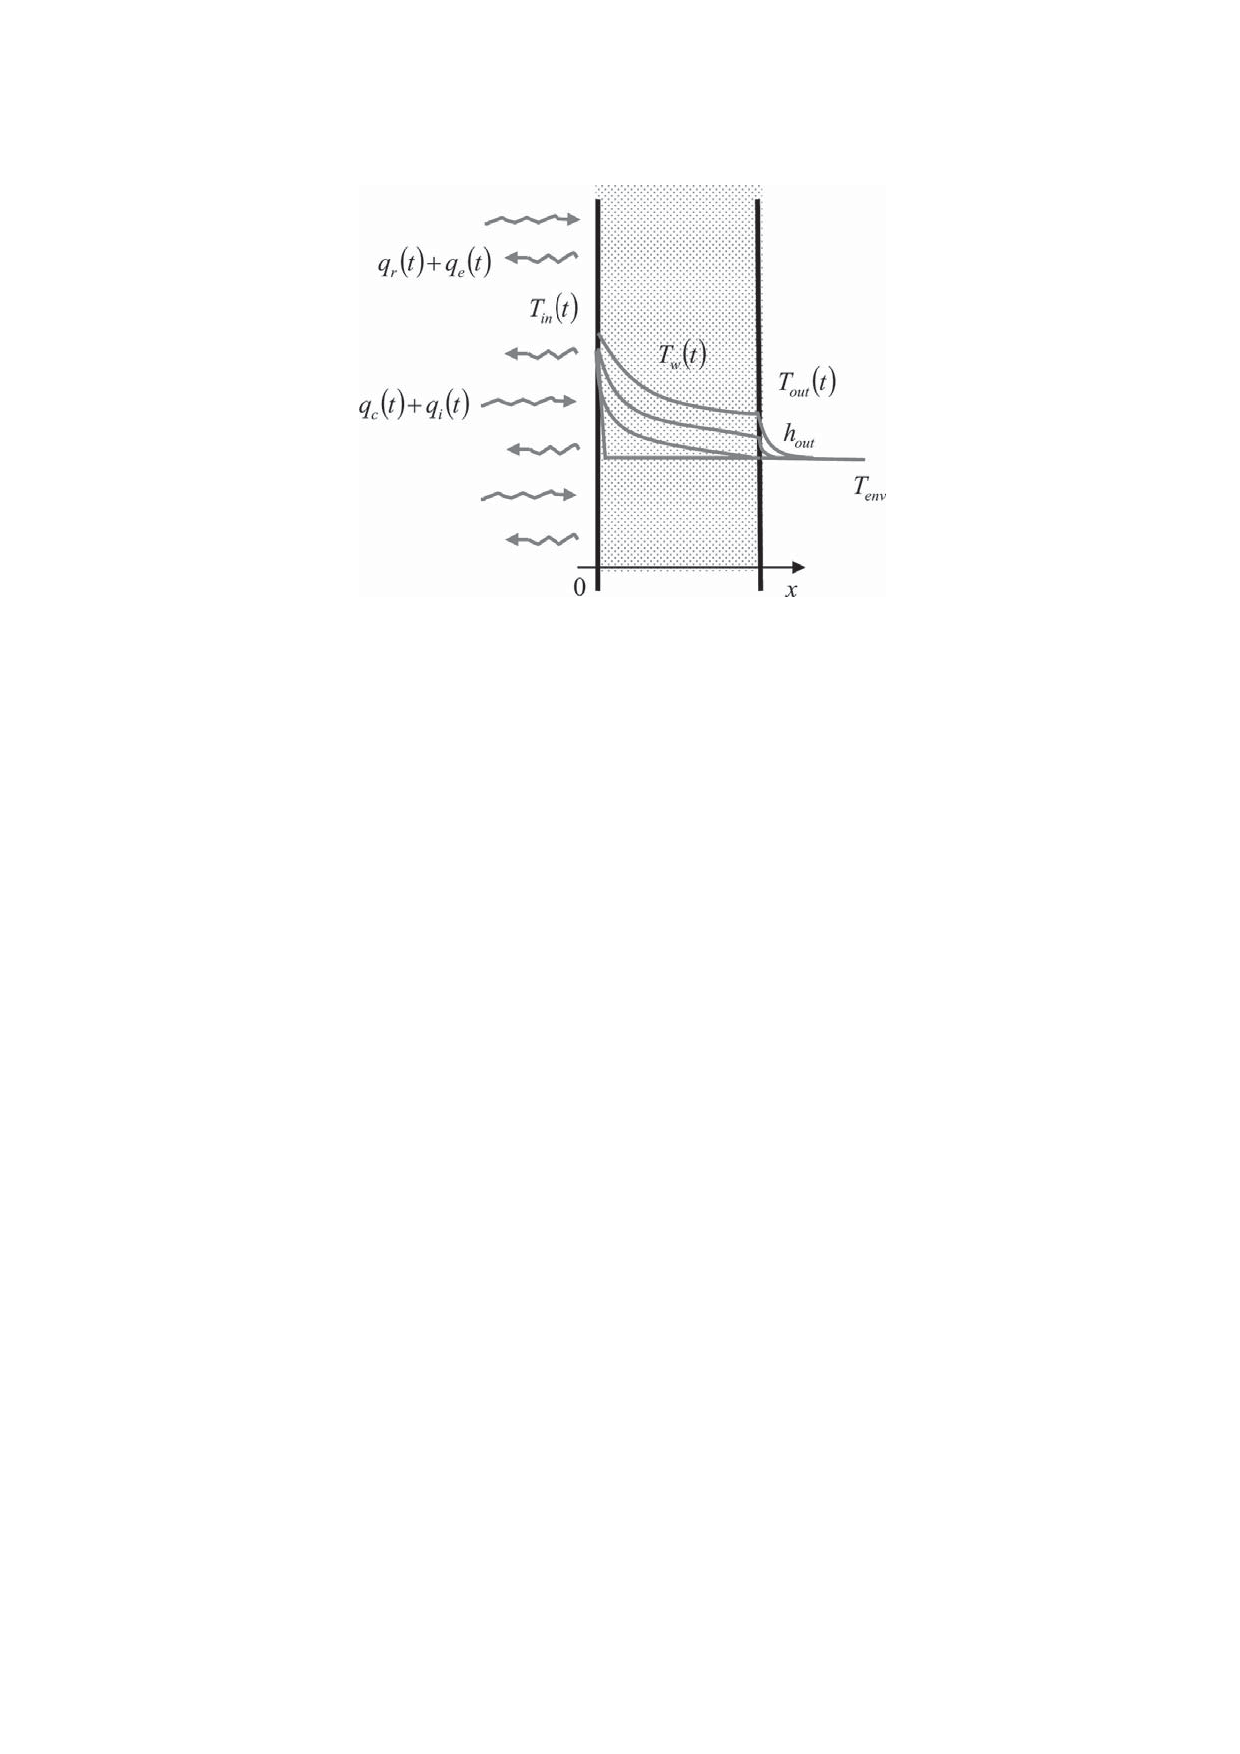
\includegraphics[scale=0.5]{horvat_model} &
			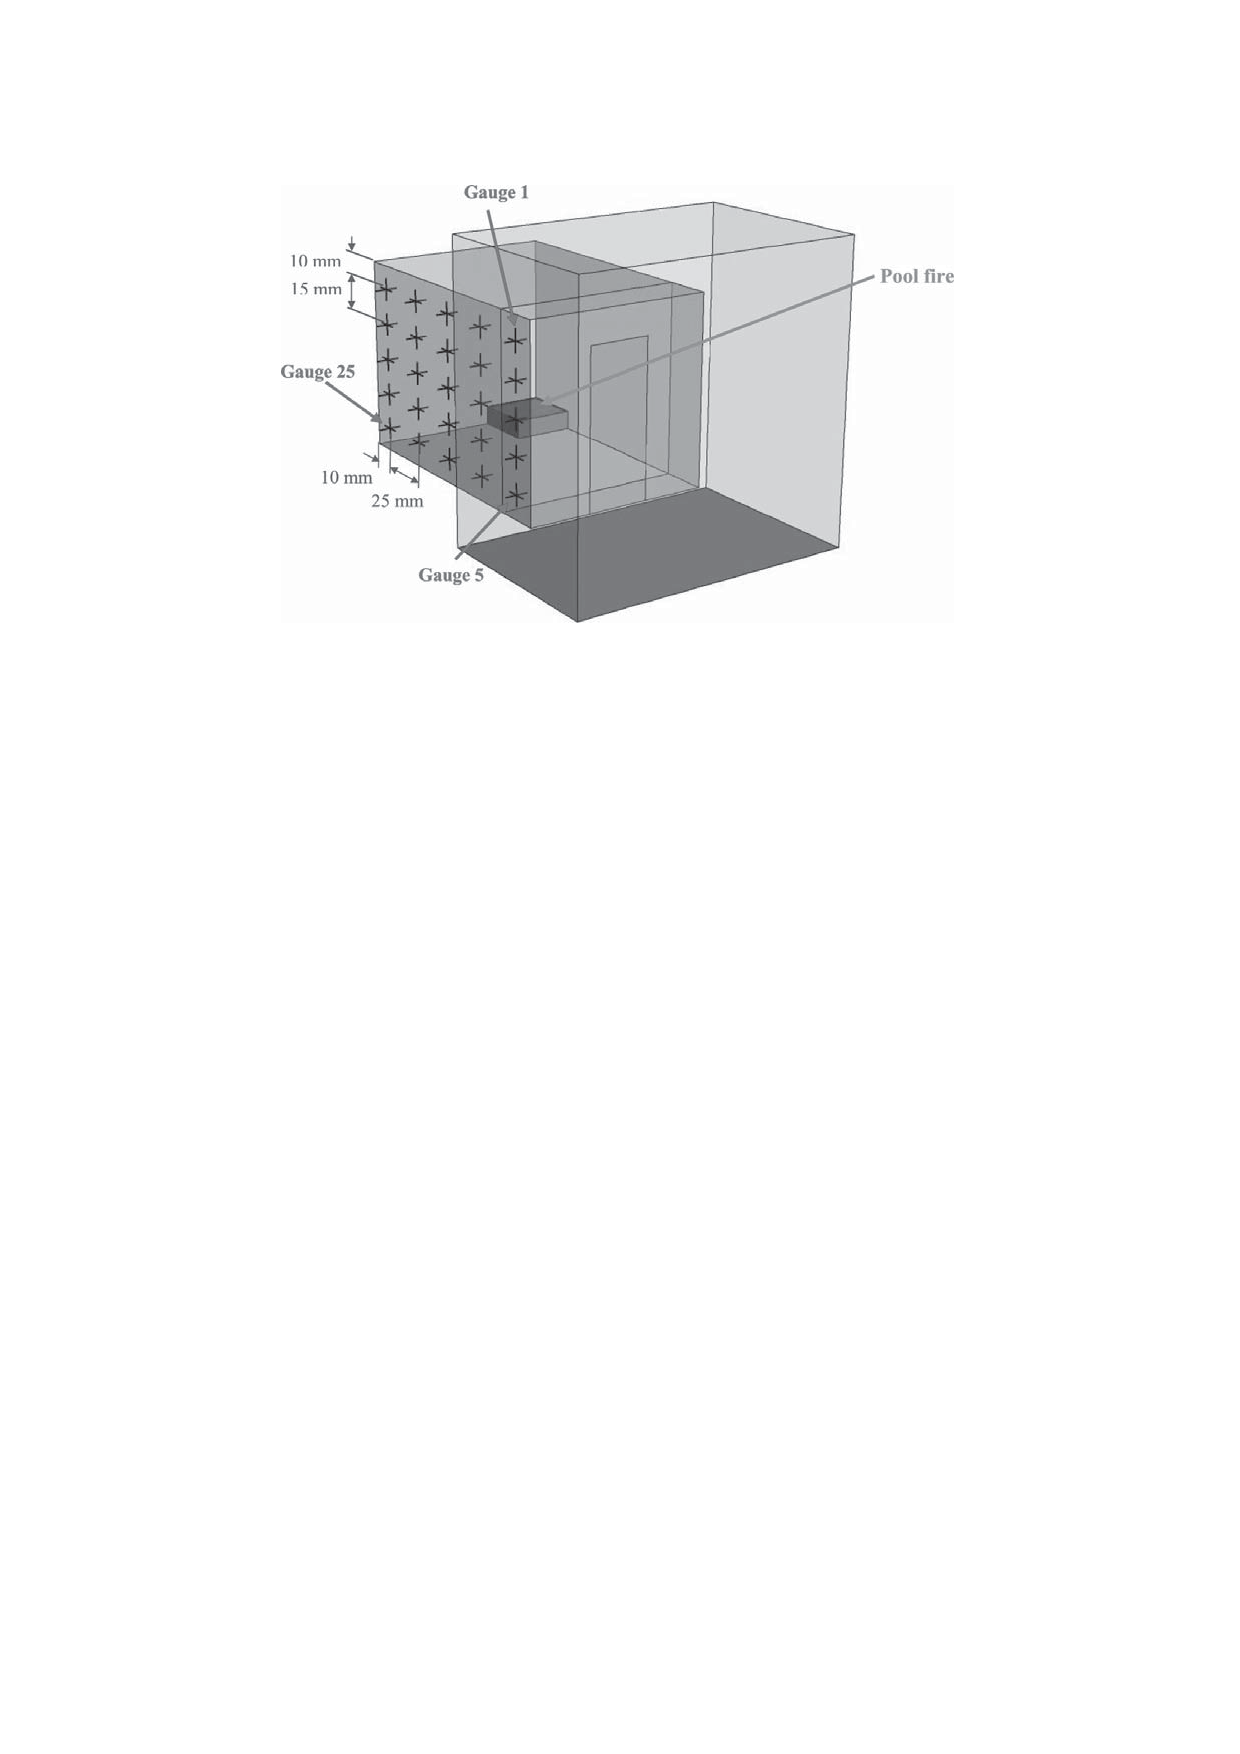
\includegraphics[scale=0.5]{horvat_domain} \\ 
			(a) & (b) \\ 
		\end{tabular} 
		\caption{Modal and domain used by \citet{Horvat2009}}
		\label{fig:horvat_model}
\end{figure}

The fuel boundary was from the back-left corner of the room with sizes of 0.25 m x 0.25 m with 8 cm elevation. Methanol was used as the fuel source for the inlet boundary condition. This combustion modelling in CFX was based on eddy-dissipation model proposed by \citet{Magnussen1977}. The emissivity of the walls was assumed to be opaque with emissivity value 0.9.

The radiation within the cavity is modelled as per discrete transport model. The thermal model of the wall considered in the numerical analysis is shown in Figure 2 11.The values of thermal heat transfer co-efficient to determine the effect of convection within the cavity were also considered. The convective heat transfer co-efficient hw varies with time. It was also reported that the heat transfer through the wall takes place by two mechanisms, one through the thermal radiation and the other through the convection of gases. Transient state heat transfer analysis was considered in this study. This developed heat transfer model was validated by comparing its results with experimental results from \citet{Tofilo2005}. The comparison showed good agreement and the benefits of this semi-analytical computational technique. 

The fire resistance of plasterboard entirely depends on the first dehydration point, which takes place at 80\degree C to 250\degree C during fire exposure. Therefore, \citet{Kolaitis2013} developed a solid reaction kinematics dehydration model for gypsum plasterboards exposed to fire to be used in CFD simulations. This research addressed the important shortcoming from previous research. The model developed included the thermos-physical properties of gypsum plasterboard (density, thermal conductivity and specific heat) and water vapour released from the plasterboard through mass diffusion and convection when exposed to fire. These effects were considered in the model to accurately predict the behaviour of gypsum plasterboards under fire. In this model, the dehydration reactions were not predicted by effective specific heat formulation, whereas two step solid reaction kinematic scheme was used for the predictions. Arrhenius equation was used to estimate the respective reaction rate. Fire Dynamic Simulator (FDS) code was developed based on the above-mentioned criteria and validated with constant thermo-physical property model and an effective specific heat model. The constant thermo-physical model is used as an effective benchmarking model in CFD problems and was used in this research. It was concluded that the proposed CFD model predicted the gypsum plasterboard behaviour with a good agreement level when compared to small-scale fire test. It was also reported that if the constant thermo-physical properties of the gypsum plasterboard are used the results showed discrepancies with the experimental results. The quantifying of the water vapour content in the model improves the prediction of the gypsum plasterboard. 

The influence of wall emissivity and convective heat transfer coefficient within the wall cavity at elevated temperatures were investigated by \citet{Andreozzi2013}. Adiabatic Surface Temperature (AST) model proposed by Wickstrom was investigated with CFD. Conjugate heat transfer analysis is a method that involves the interaction of thermal and structural analysis within the same software. Since this method is computationally very expensive, the AST method is preferred. The AST method used in this study consists of two steps. In the initial step, the thermal analysis was carried out with CFD and later the net heat flux obtained as a result from CFD was transferred to FEM for structural analysis. In this research conjugate heat transfer analysis and standalone beam analysis were carried out under similar fire exposure and the results were compared. Good agreement was observed between the experimental results and the model when the AST was used as the parameter to transfer CFD results to structural model. The geometry of the model considered was 3 m \(\times\) 3 m with four openings of 20 cm on all sides of the wall.

\citet{Arendt2014} developed a fully transient model of heat transfer in buildings. Transient envelope model and transient CFD model were used to develop this heat transfer model. Reynolds-averaged-Navier-Strokes (RANS) equation was utilized in this research. Higher Reynolds number was used to make the meshes coarser to reduce the computational time during the heat transfer analysis. It was assumed from the CFS solution that, there existed a surface-averaged and time-dependent heat transfer coefficient for a given surface. This study was conducted by considering a room with walls possessing thermal capacitance and single ventilation. Developing a transient coarse meshed CFD (RANS) model and transient heat transfer in the building was the principal focus of this research. From the outcomes of this research, it was concluded that the proposed CFD method can be used in reducing the analysis time.

\citet{Lazaro2016} studied the variations in the thermal models used for gypsum plasterboard assemblies in a standard fire test. Numerical models were compared with the experimental results and discrepancies in the current thermal models were reported. Experiments were conducted to determine the thermal and mechanical properties of fire rated gypsum plasterboards. Four full scale fire tests 3 m \(\times\) 3m were conducted with different configurations. Three fire tests consisted of single row of studs, whereas one test consisted of double row of studs separated by air gap. All the fire tests were conducted under non-load bearing conditions in accordance with Eurocode EN 1363 and EN 1364. Two layers of plasterboards were used for three tests and four layers of fire rated plasterboards were used for one test. Sudden increase in temperature profile was observed on the ambient face of the LSF wall panel after the first plasterboard layer fall-off in tests with two layers of plasterboards. This was found to be the combined effect of ablation causing convection of hot air within the cavity. Fire Dynamics Simulator (FDS) was used in the numerical study. The model size was 50 \(\times\) 50 mm\(^2\) with 5 mm mesh size. Ablation was considered at the third peak reaction corresponding temperature of gypsum in the numerical model. Apparent thermal properties were used in the model to match the numerical results with the experiments. A new hypothesis was proposed by assuming that the ablation in the plasterboard occurs at about 360\degree C which was considered as the third endothermic reaction point. It was concluded that the approximation of the thermal properties was held valid for numerical models with two layers of plasterboards. In the case of wall specimen with four layers of plasterboards, the numerical model results did not match well with the experimental results. This is because, the thermal conductivity between the interface of the plasterboards is difficult to determine causing the discrepancy. Although this research modelled the fire behaviour of LSF walls with CFD only the non-load bearing LSF walls were considered for both experimental and numerical investigations. Also, the temperature gradient along the width of the wall panel was not investigated. The numerical model was validated by comparing the ambient side plasterboard temperatures only.

\citet{Thanasoulas2016} investigated the heat transfer through CFS wall systems through ANSYS CFX software. Structural analysis was carried out on ADINA to determine the structural failure of the CFS walls. Transient heat transfer analysis technique was used for the ANSYS CFX model. Sequentially coupled analysis approach was followed in this study, where the thermal analysis is conducted first and the output is transferred to the structural analysis in the later stages. The models were validated against experiments conducted by \citet{Gunalan2013e} and also the FE models developed by \citet{Gunalan2013f}. 2D conduction elements were used for the heat transfer model and the thermo-mechanical properties for the thermal and structural analyses were extracted from \citet{GhaziWakili2007,Kolaitis2013}. A plateau region was observed on the time-temperature curves during the gypsum dehydration process when exposed to standard ISO fire curve. It was reported that the plateau region happens at 80\degree C which is debatable. Shell elements were used for structural modelling, wherein the temperature inputs from the thermal analysis was keyed in to perform linear and non-linear analyses. Geometric and material non-linear imperfections were included in the structural model. Total of four full-scale fire tests were considered for the purpose of model validation. It was concluded that, based on the numerical simulations, cavity insulation with mineral wool did not significantly alter the FRL in comparison with non-cavity insulated wall specimen under load bearing conditions. Whereas, the usage of multiple layers of plasterboard did have considerable effects on the FRL under load bearing conditions. The limiting temperature of 350\degree C was found to be conservative for the design of steel studs as the stud load-bearing capacities were satisfactory at the limiting temperature.      

\citet{Malendowski2017} developed a coupling method for CFD-FEM analysis of steel structures exposed to natural fire. Scripts were developed to translate the CFD results into transient boundary condition in FE analysis. The CFD code JASMINE was coupled with an FE code SAFIR. Convective and radiative heat flux are given as an input to the FE model. A compartment with dimensions 8 m x 20 m and 3.20 m high was considered for the computational model as per a full scale fire test conducted by \citet{Pyl2012}. FDS and ABAQUS input files were generated with scripts from Scilab software. UTEMP subroutine was used for defining the boundary conditions in ABAQUS. This UTEMP subroutine was used to create the non-uniform temperature boundary condition in ABAQUS because of heat transfer analysis results from FDS. Real fire curves were used in this study as per \citet{Pyl2012} rather than the fire curves used in the furnace fire tests. This is because the non-uniform radiative heat transfer on the structural elements in the case of a real fire exposure. Pool fire scenario and equally distributed fires were used in the numerical analysis and the results agreed well with experimental results. It was found that the distributed fire scenario is more intense when compared to the local fire by over four times. The deformation plots from structural analysis for both fire scenarios agreed well with the experimental results. 

\citet{Thanasoulas2018} extended the modelling techniques to develop a fully coupled model, to investigate the thermal and structural response of CFS drywall systems. 3-D solid elements were used for modelling the plasterboard, steel studs and insulation to simulate heat transfer through the thickness and also to simulate the structural response in a coupled way. ADINA was used as the software package for the analyses. All the structural elements including the fasteners were modelled to the thermo-mechanical analysis. Appropriate thermal and structural boundary conditions including contact interaction properties were specified along with the elevated temperature material properties. Thermal properties of air was also taken into consideration for the thermo-mechanical analysis. The analysis results showed that the FRL of LSF walls with cavity insulation was higher in comparison with non-cavity insulated LSF walls which is highly debatable as other past research show that the presence of cavity insulation significantly reduces the FRL in LSF walls. 

\section{Literature Review Findings}
The following findings are derived from the conducted extensive literature review.
\begin{itemize}
	\item Fire performance is considered as an important parameter for walls in LSF constructions. The quantum of research data on the fire performance of LSF walls is extensive supporting this claim. However, there prevails substantial gaps in this research area, where the fire performance under different fire curves and configurations is still not investigated in detail. 
	\item Experimental investigations were conducted extensively on simple LSF wall configurations. The tested walls included single row of studs sandwiched between plasterboards of different materials and thickness. This also included the variation in steel stud thickness and also grade of steel. But, only single row of studs were used in all the experimental investigation. LSF wall configurations with complex stud arrangements were investigated only by very few researchers and the fire test data is not readily available as well.
	\item Attempts were made to improve the FRL of LSF wall systems by changing various parameters. This includes, increasing the plasterboard layers on both the fire exposed and unexposed sides, changing the type of insulation used within the cavity and using different geometric configurations in the studs. But, attempts were not made in relation to increase the complexity of wall system by altering the stud arrangement in the LSF wall system. This forms a vast research gap in determining the heat transfer mechanism in LSF walls with complex stud arrangements. The presence of more than one row of stud will result in increased cavity depth and can change the heat transfer mode in comparison with a conventional single stud LSF wall.
	\item Many research studies have been conducted on the effect of plasterboard restraints under load bearing conditions provided to the studs under fire and ambient conditions. However, this effect was investigated on single stud LSF walls only. In case of complex LSF walls, the effective plasterboard restraints vary vastly in certain complex LSF wall configurations. This phenomenon has to be explored in detail and necessitates the need for experimental investigation on the fire performance of complex LSF walls. Also, during a fire test, the LSF wall is subjected to thermal bowing. This effect results in neutral axis shift providing additional bending moments to the LSF walls under axial loading. The thermal bowing effect is investigated in detail for LSF walls with single row of studs only. However, these effects are not investigated in detail in complex LSF walls.    
	\item Based on past experimental and numerical research studies, the stud hot flange limiting temperatures have been predicted for different single stud LSF wall configurations. This include cavity insulated and non-cavity insulated LSF walls. Through the limiting hot flange temperatures, the FRL of a given configuration can be easily derived with reasonable accuracy. But, no such data is available for the complex LSF wall configurations. Therefore, it becomes a necessity to investigate the stud hot flange temperatures in complex LSF wall configurations and determine if the existing stud hot flange limiting temperatures are suitable to predict the FRL of the complex LSF wall configurations. 
	\item The numerical models developed to predict the heat transfer in LSF walls were through software packages such as SAFIR, ABAQUS, ANSYS, ADINA and FDS. The models were created using 2D and 3D elements and predictions were made to validate the models against experimental results. However, there does not exist a robust numerical model that can precisely predict the heat transfer mechanism in complex LSF wall configurations. Some of the existing heat transfer models included only radiation mode of heat transfer within the cavity and could still validate the time-temperature curve predictions from the experiments. However, in LSF walls all three modes of heat transfer which includes conduction, convection and radiation happens within the cavity. Only numerical models created with CFD software packages could account for these effects. The packages such as ANSYS-FLUENT, ADINA and FDS were used by past researchers for developing heat transfer model using CFD techniques, but the former mentioned packages such as ANSYS and ADINA are commercial versions and involves a licence cost while FDS is an open source package. Therefore, FDS is found to be the better alternative to develop heat transfer models for this research study.
	\item Structural models were also developed by past researchers to predict the structural failure modes under ambient and elevated temperatures. These models were either sequentially coupled and executed after the thermal analysis or fully coupled and executed alongside the thermal analysis to predict the FRL of LSF walls. However, the fully coupled models were found to be computationally expensive and time consuming. Therefore, sequentially coupled analysis is found to be comprehensive and preferred method, where the temperature data is extracted from thermal analysis and used for structural analysis.
	\item Numerical models were found to be the most feasible option to predict the FRL of LSF walls. However, the quantum of computational resources and technical skills to conduct these analyses are challenging. Therefore design equations were made available in various standards such as AS/NZS 4600 and Eurocode 3, Part 1.2. Developed design equations based on the existing standards pertaining to LSF walls were also developed by past researchers. There exist alternate methods such as finite strip analysis, DSM and EWM to predict the FRL of LSF walls to reasonable accuracy. This research will focus on checking the suitability of the existing design equations and their applicability in predicting the FRL of complex LSF walls.
	\item The design equations rely on the hot and cold flange temperatures arrived either from experiments or from numerical studies. In single stud LSF walls past research studies assume a constant temperature on the hot and cold flanges while the web temperatures are assumed to be linearly varying. This assumption holds good for LSF wall with single row of studs and the FRL predictions from design equations match reasonably well with the experimental results. However, in complex LSF wall configurations, there exists more than single row of studs and the applicability of this assumption is debatable. Therefore, extensive experimental and numerical studies becomes necessary to determine the amount of variation in the temperature gradient along the studs. This data can then be used in the design equations to predict the FRL of complex LSF wall configurations.  
\end{itemize} 

\chapter{Experimental Investigations under Ambient Conditions}
\label{ch:Ambient}       
\section{General}

This chapter details the experimental investigations conducted on complex LSF wall systems under ambient conditions. Despite the advancements in numerical models, experiments are necessary to determine the ambient load carrying capacity and the robustness of developed FE models to predict the axial load carrying capacity of the complex LSF wall systems. Also, the capacity of walls at ambient temperatures are required to conduct full-scale fire tests under load bearing conditions in which as a percentage of the ambient axial capacity of the wall system is applied during fire tests. Therefore, experimental investigations were carried by conducting ambient capacity tests and the ambient load carrying capacity of the complex LSF wall specimens were determined. Tensile coupon tests were also conducted on the steel studs to determine the yield strength of the studs which will later be used for the numerical analyses and parametric studies.  

\section{Ambient Capacity Test Setup}

Ambient capacity tests are used to determine the axial load carrying capacity to be used for the fire test in accordance with AS 1530.4. However, the testing procedures to determine the ambient capacity is not detailed clearly in the aforesaid standards. Therefore the tests were conducted similar to full-scale fire tests without the fire load. The ambient capacity tests were conducted on a specially built test frame which can accommodate specimens up to 3 m \(\times\) 3 m in external dimensions. The test frame consists of two Universal Columns (UC's) fixed to the strong floor. At the top the columns are connected through a Welded Beam (WB) and at the bottom through a Universal Beam (UB) resting on the floor. Individual hydraulic ramps were used to load the test wall at the stud locations and are placed on the bottom Universal Beam (UB). The test specimens are loaded from the bottom rather than the top for the ease of experimental set up. LSF wall specimens are constructed on a mounting table held on to the ground. After construction, the test specimens are loaded into the test frame using forklift and Electric Overhead Travelling (EOT) crane. Linear Variable Displacement Transducers (LVDT's) were used to measure the axial displacement and lateral deflection at various locations during the test. The axial displacements were measures at the bottom loading plate near the rams. Lateral deflection was measured at three locations in critical studs which include the 750 mm from the top and bottom of the specimen and also at mid-height of the specimen. Details of a typical test specimen and the loading frame is shown in \Cref{fig:typical-ambient}.
\begin{figure}[!htbp]
	\centering
		\begin{tabular}{c}
			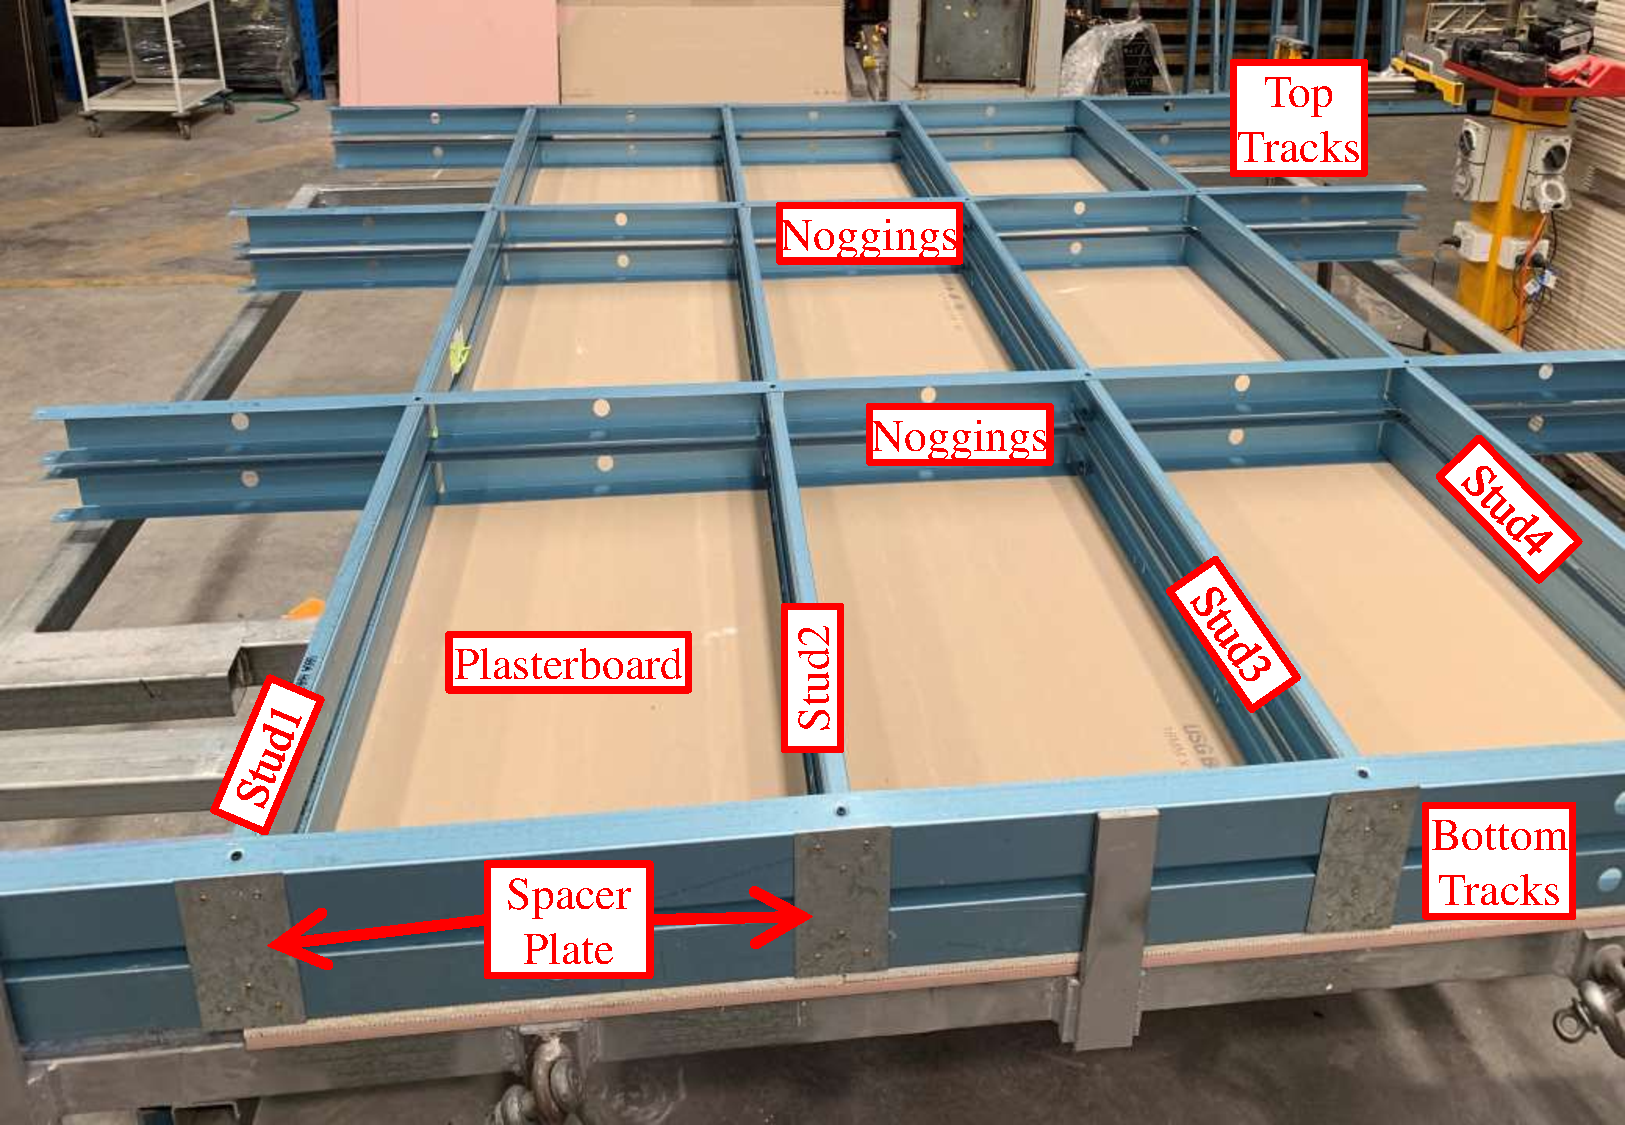
\includegraphics[scale=0.3]{ambient_construction.pdf} \\
			(a) \\
			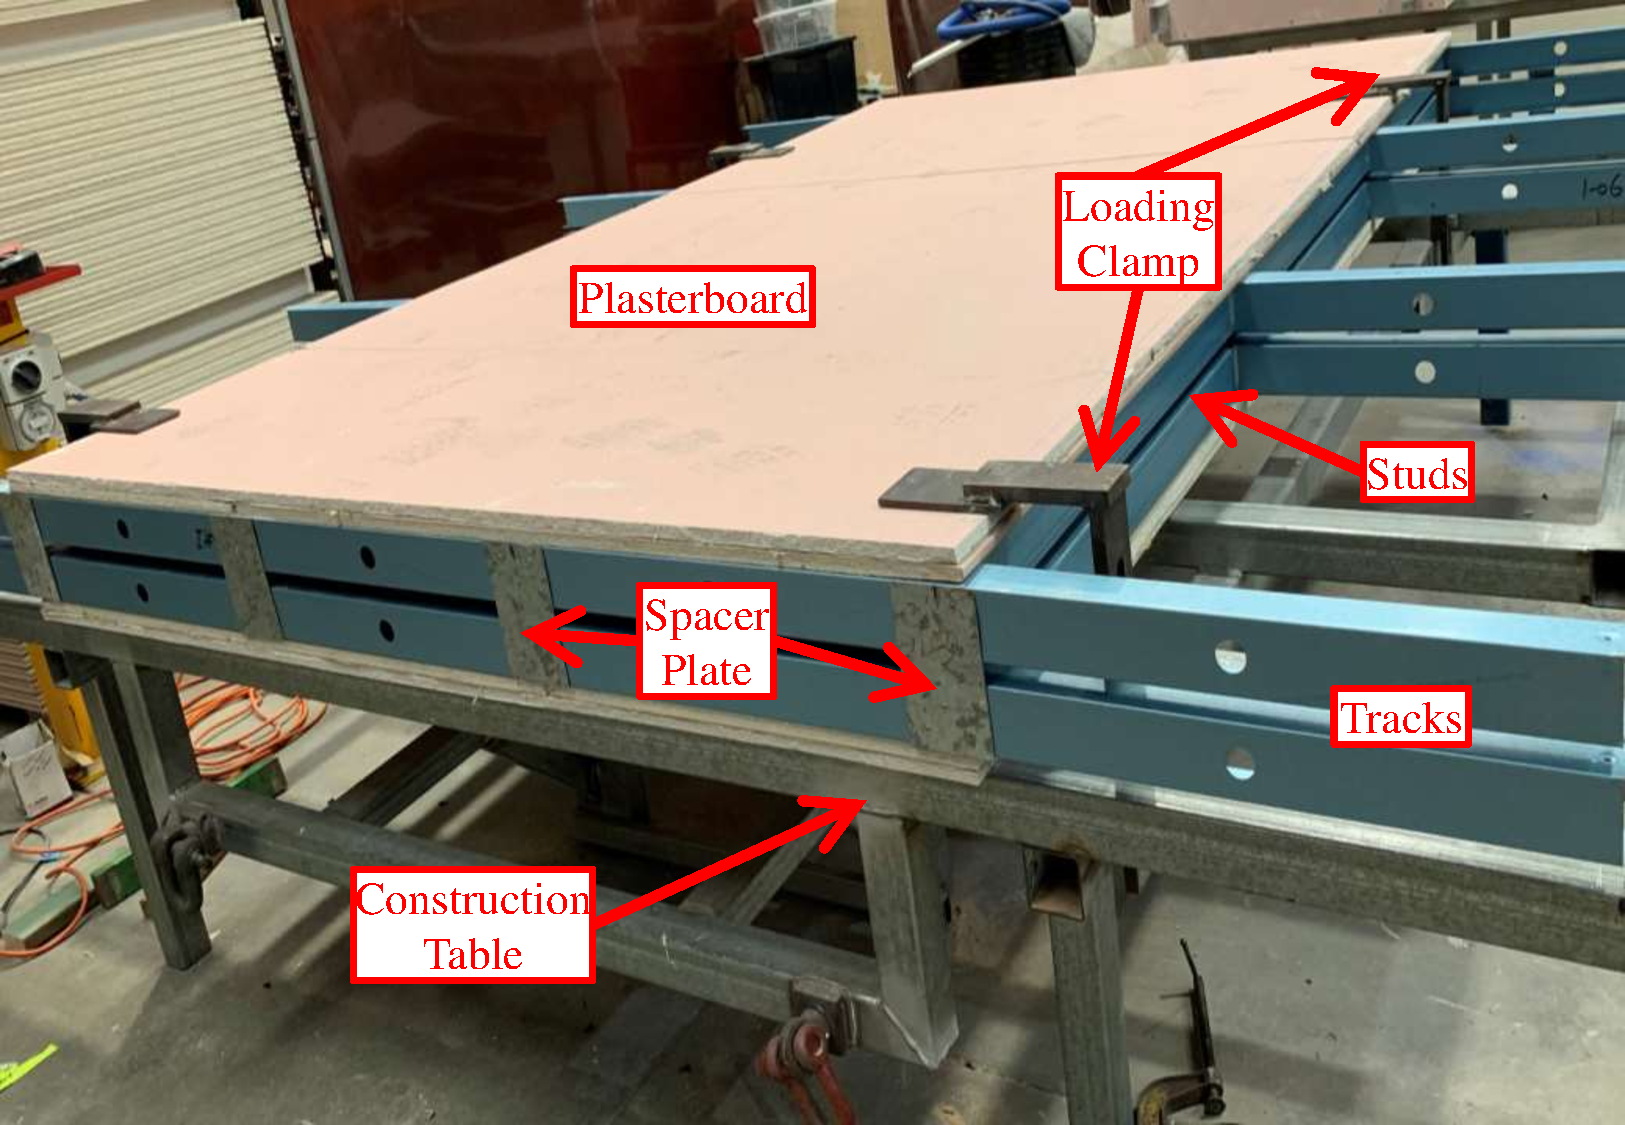
\includegraphics[scale=0.3]{ambient_finished.pdf} \\ 
			(b)  \\
			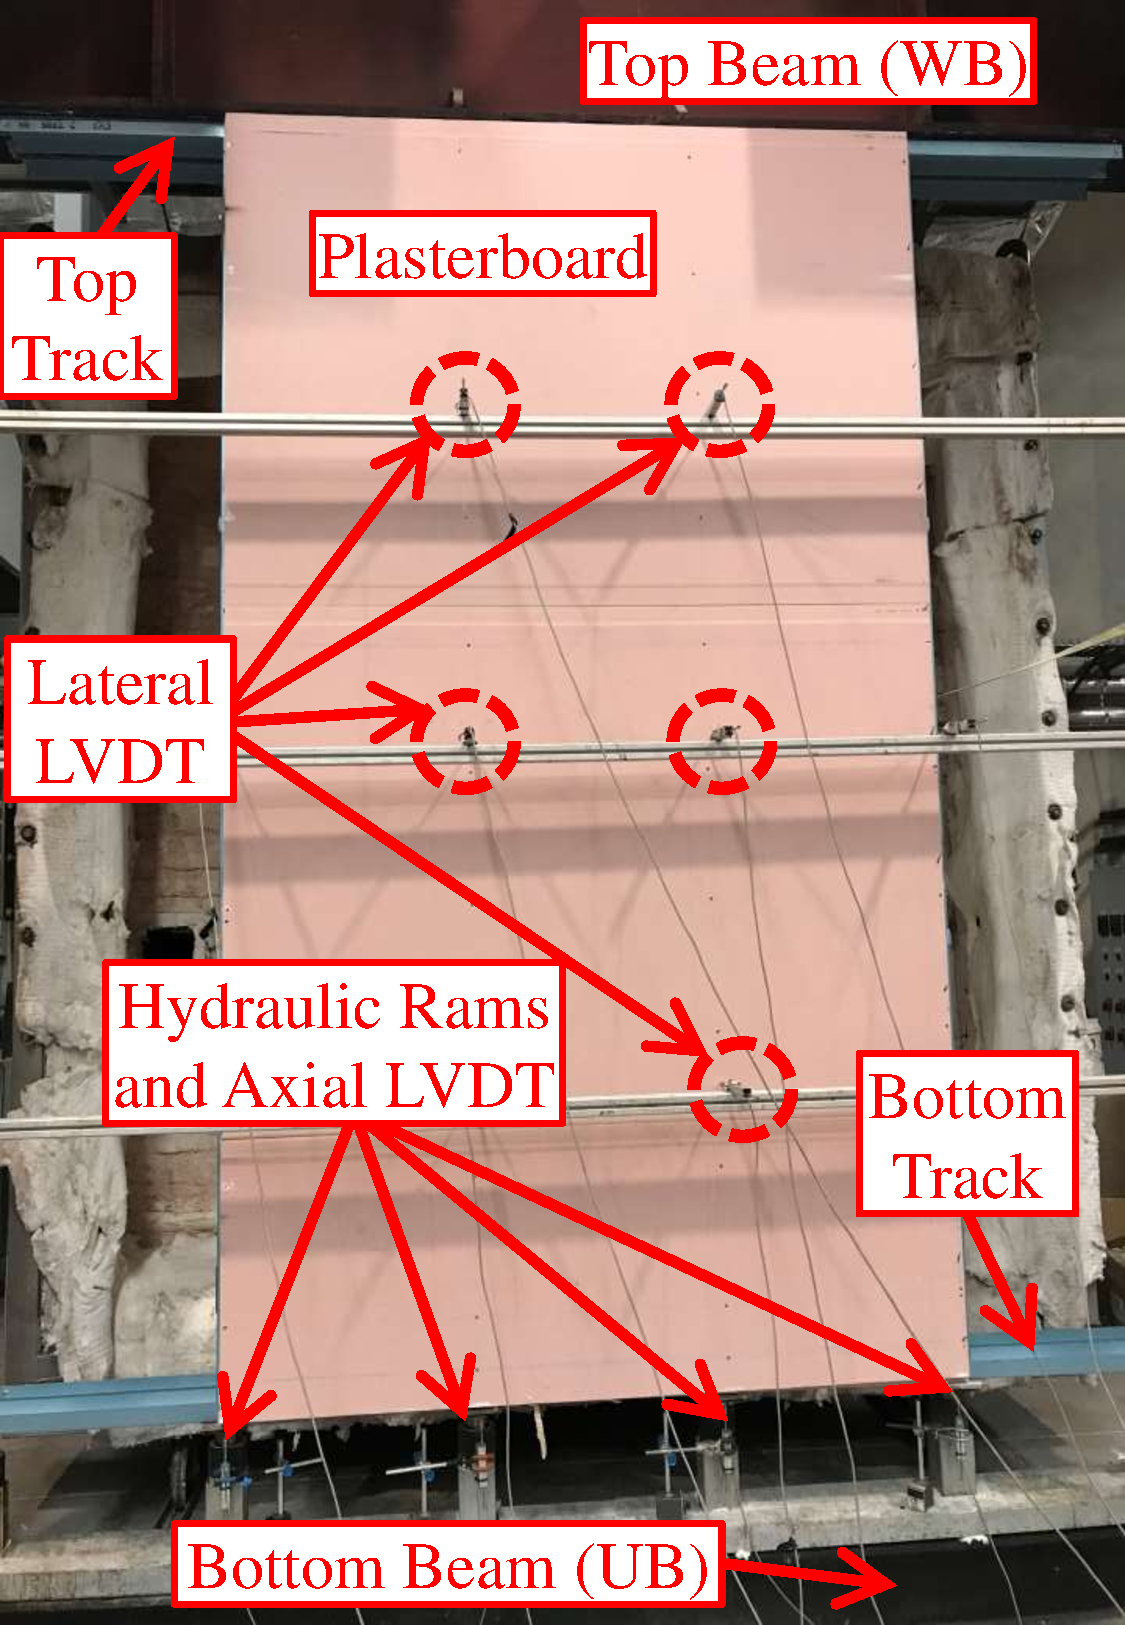
\includegraphics[scale=0.25]{typical_ambient.pdf}\\
			(c)  \\ 
		\end{tabular} 
		\caption{Typical experimental set-up of ambient stud wall (a) Construction of the test wall (b) Finished test wall (c) Loaded test wall}
		\label{fig:typical-ambient}
\end{figure}

A summary of the ambient capacity test conducted as a part of this research study is presented in \Cref{tab:ambient-test-specimens}. All the test specimens had Lipped Channel Sections (LCS) as studs made of G550 steel manufactured by Bluescope with a minimum guaranteed yield strength of 610 Mpa. The steel studs had pre punched holes drilled on them at required positions for easier construction. Buildex M6.0 \(\times\) 15 GX Ca smooth top GA point steel frame screws were used to connect the steel studs to the tracks and noggings. Unlipped Channel Sections (UCS) were used for the top and bottom tracks and pre punched holes were made in the flanges of the tracks and corresponding locations to fix the studs. UCS were used as noggings at 1 m intervals in all the tests but for Test-AT5. However, the UCS noggings were replaced by omega noggings and details about the same are provided in the corresponding section.
\begin{table}[!htbp]
	\centering
	\caption{Ambient test panel details}
	\begin{tabular}{cccccc}
		\toprule
		\multicolumn{1}{m{2.4em}}{\centering{Test Name}} & 
		\multicolumn{1}{m{5.6em}}{\centering{Description}} & 
		\multicolumn{1}{m{2.85em}}{\centering{Stud Depth (mm)}} & 
		\multicolumn{1}{m{2.85em}}{\centering{Cavity Depth (mm)}} & 
		\multicolumn{1}{m{5em}}{\centering{Stud Thickness (mm)}} & 
		\multicolumn{1}{m{3em}}{\centering{No of Studs}} \\
		\midrule
		AT1  & Double Stud & 90 & 200 & 0.95 & 4 \\
		AT2  & Double Stud & 90 & 200 & 0.75 & 4 \\
		AT3  & Double Stud & 90 & 200 & 0.75 & 6 \\
		AT4  & Double Stud & 70 & 160 & 0.95 & 4 \\
		AT5  & Staggered Stud & 90 & 200 & 0.95 & 6 \\
		\bottomrule
	\end{tabular}%
	\label{tab:ambient-test-specimens}%
\end{table}%

All the test specimens were lined with two layers of 16 mm fire rated gypsum plasterboard. The plasterboards were connected to the stud flanges through D type 10 GA self-piercing screws. The first layer of plasterboard was fixed to the studs using 32 mm long screws while the second layer was fixed using 45 mm long screws. The plasterboards joints were not seals with joint compound as the corresponding effect on ambient load carrying capacity is negligible. The plasterboards were fixed with a screw spacing of 200 mm at joints in a staggered manner while linear arrangement with 300 mm spacing was adopted at the edges and at plasterboard centres. A 60 mm gap for first layer and 80 mm gap for second layer of plasterboard was provided to prevent plasterboards being screwed on to the top and bottom tracks to allow for axial compression expansion during the tests. Description about the variations in the individual ambient capacity tests and their corresponding results are discussed next.

\section{Ambient Test-AT1}\label{sec:AT1}

The first ambient capacity test was conducted on double stud LSF wall with 90 mm studs. Grade 550 steel with dimensions of 90\(\times\)36\(\times\)7\(\times\)0.95 were used as studs. 90 mm unlipped channel sections were used as noggings at 1 m intervals. The noggings were connected to the studs through slots made on the webs of the UCS. Top and bottom of the test specimen were connected through 90 mm unlipped channel sections. It is to note that, the test wall had two rows of studs separated by a 20 mm gap between the studs as shown in \Cref{fig:AT1-plan}. Four studs were used for the ambient capacity test and the edge studs were strengthened to induce failure on the middle studs as the plasterboard provide effective in-plane restraints only to the middle studs. The height of the specimen was 3 m while the width was 1.8 m.  
\begin{figure}[!htbp]
	\centering
			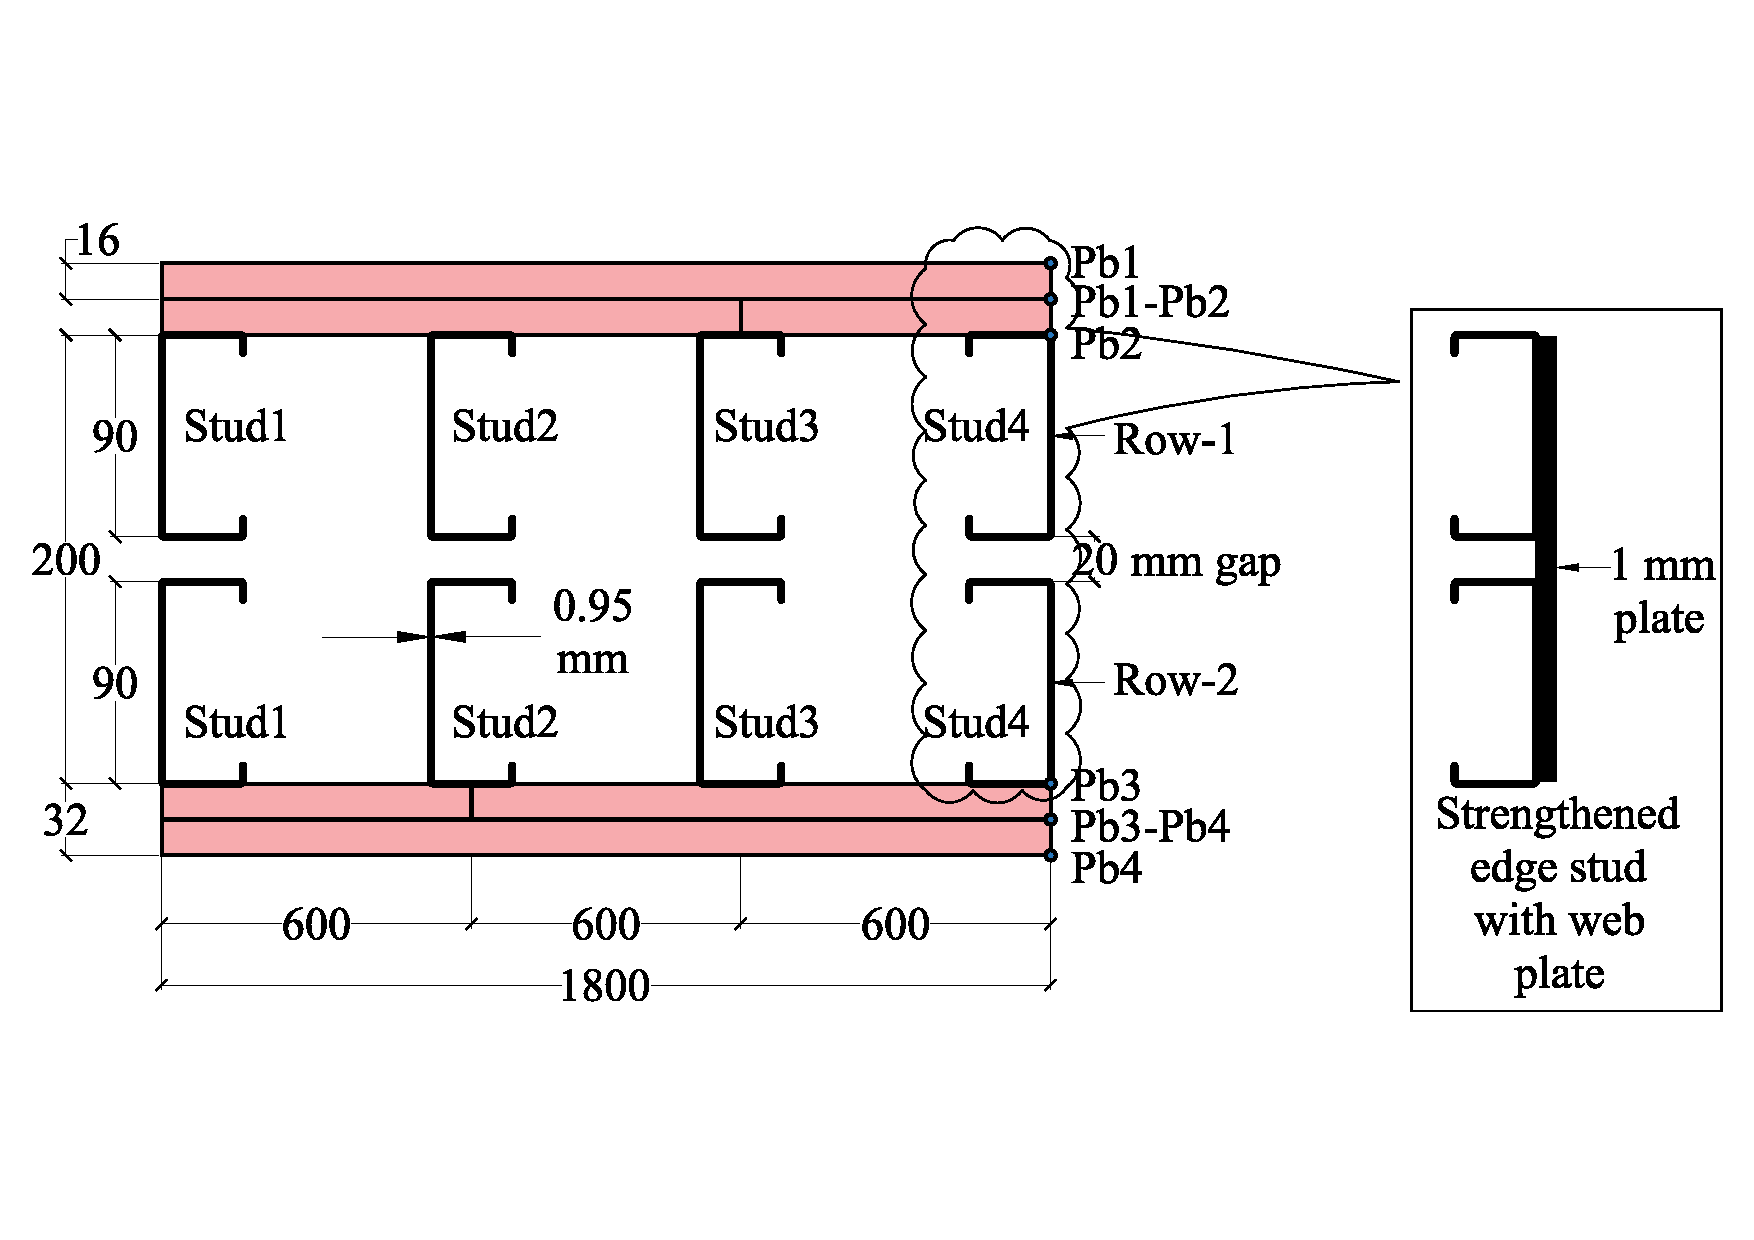
\includegraphics[scale=0.25]{AT1-plan.pdf}\\
		\caption{Test-AT1 configuration}
		\label{fig:AT1-plan}
\end{figure} 

Firstly, the test specimen was loaded to 10\% of the predicted ambient load carrying capacity for two cycles before commencing the ambient capacity test to relieve internal stresses developed in the specimen due to the construction process. After this the ambient capacity test was carried out by applying the load on the geometric centre of the studs through individual rams as shown in \Cref{fig:typical-ambient}.
\begin{figure}[!htbp]
	\centering
			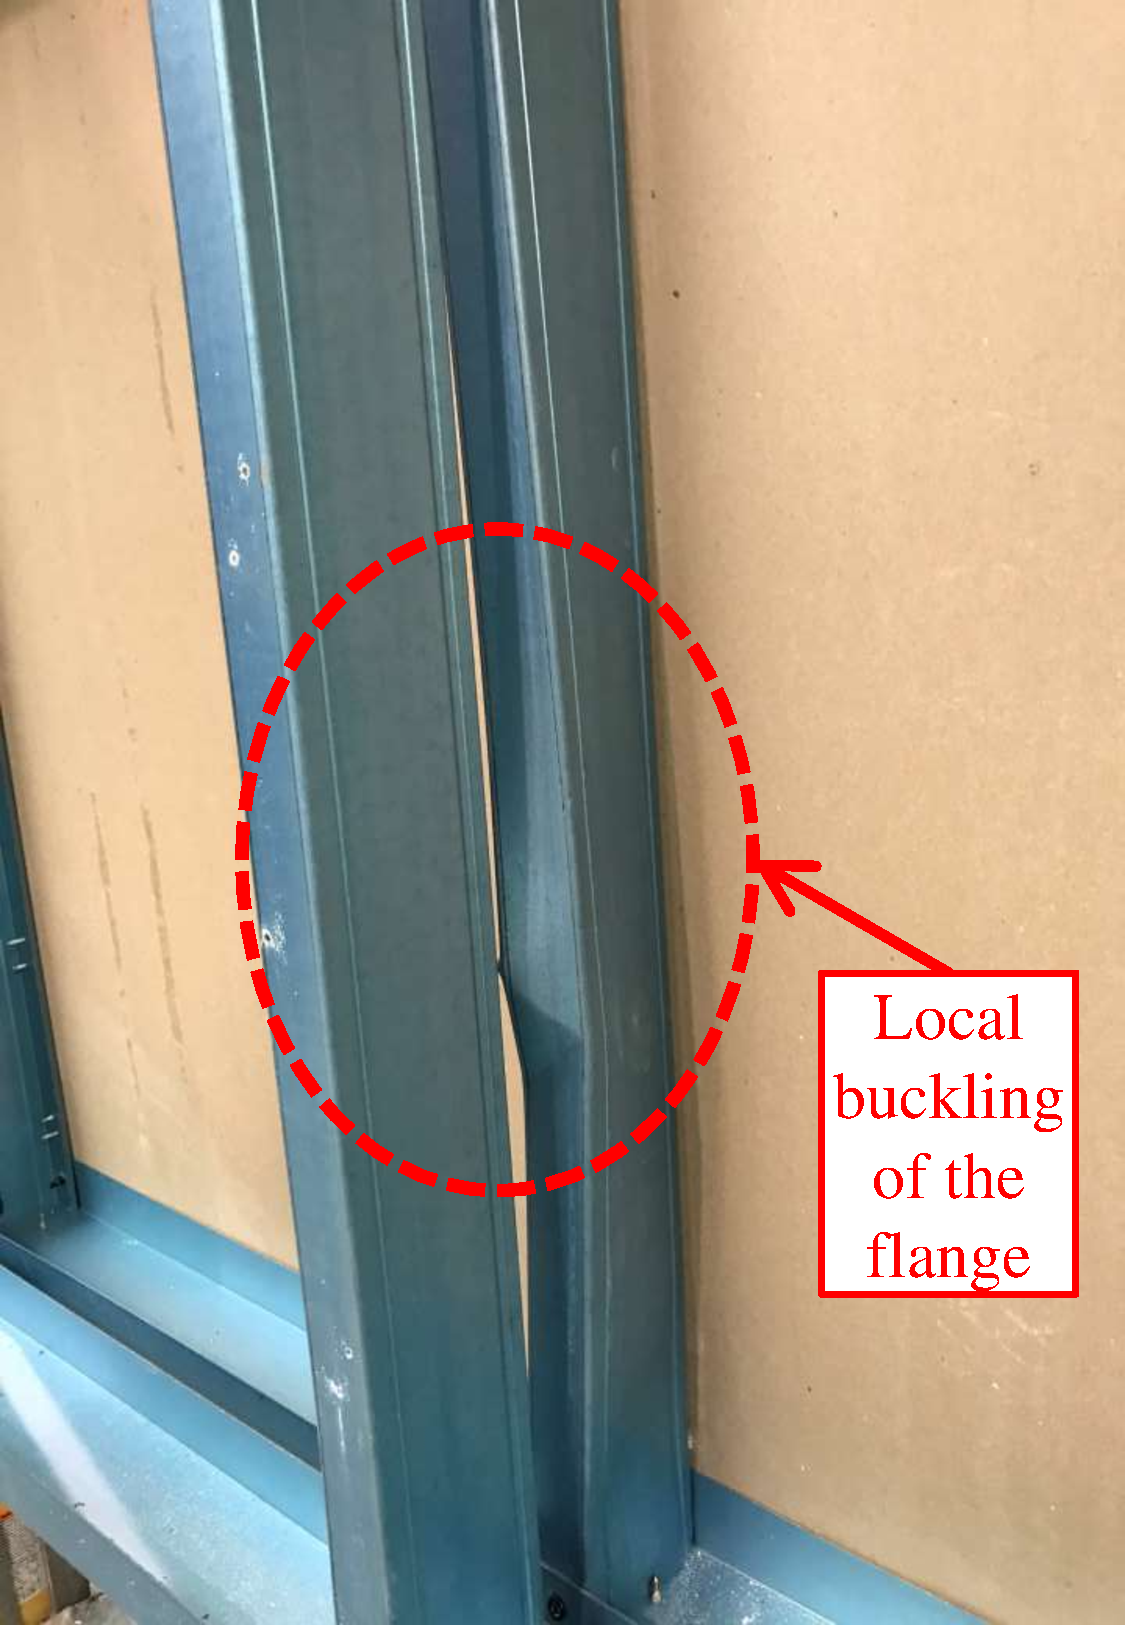
\includegraphics[scale=0.2]{AT1-buckling.pdf}\\
		\caption{Local compressive failure in test-AT1}
		\label{fig:AT1-buckling}
\end{figure} 

The ambient Test-AT1 resulted an ultimate capacity of 73 kN. Local buckling of the studs was observed in the flanges as shown in \Cref{fig:AT1-buckling}. No pull-out of the plasterboard screws were observed during the ambient capacity test. The load versus axial displacement and load versus lateral deflection curves are shown in Figures~\ref{fig:AT1-results}~(a)~and~(b). The maximum axial displacement was recorded as 13.28 mm in Stud2. Generally, in ambient capacity tests the application of load is  continued till the ultimate failure load is reached after which the applied load transferred to the studs in which buckling has not been initiated. This results in excessive post-buckling failures in some studs during the ambient capacity tests. Post-buckling failures are noticeable in Stud4 due to the additional load acting upon them as Stud2 has already buckled initially. This is evident in the load versus axial displacement curve where a maximum of 25.78 mm displacement was observed in Stud4 as shown in \Cref{fig:AT1-results}~(a).
\begin{figure}[!htbp]
	\centering
		\begin{tabular}{cc}
			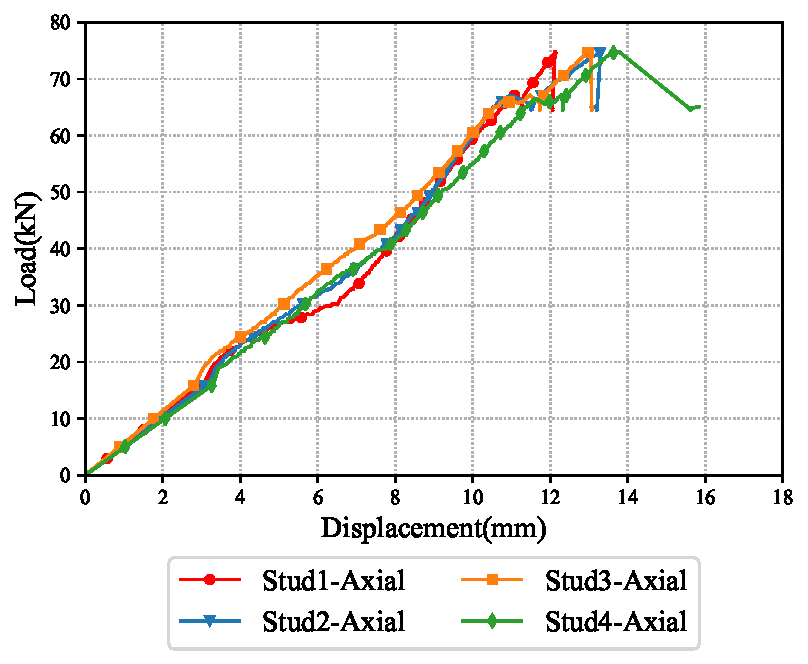
\includegraphics[width=6.5cm,height=6cm]{AT1-Load-Axial-Corrected.pdf} & 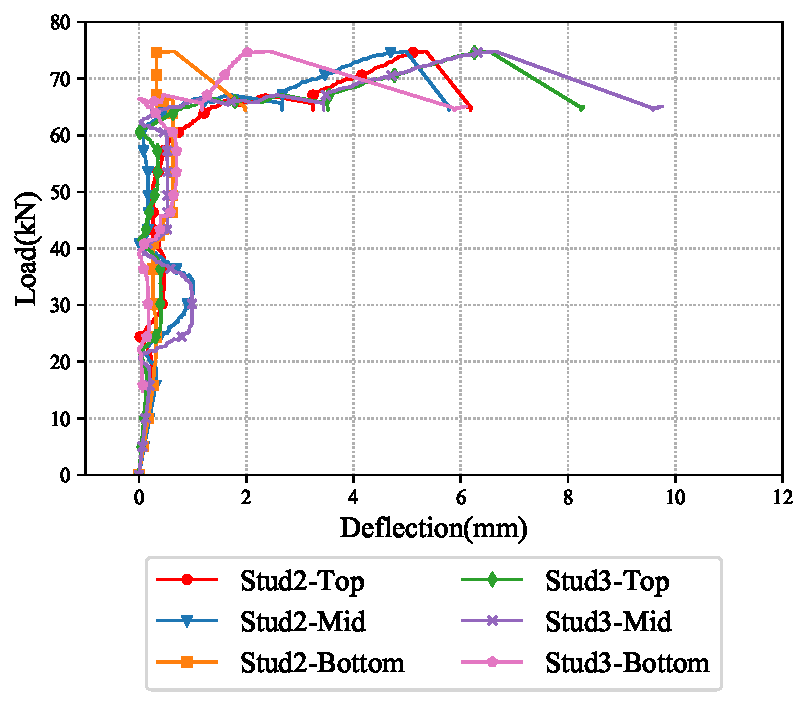
\includegraphics[width=6.5cm,height=6cm]{AT1-Load-Lateral-Corrected.pdf} \\ 
			(a) & (b)  \\ 
		\end{tabular} 
		\caption{Test-AT1 results - (a) Axial displacement and (b) Lateral deflection versus applied axial load}
		\label{fig:AT1-results}
\end{figure}

\section{Ambient Test-AT2}

The second ambient capacity test was conducted on thinner stud sections (0.75 mm) with stud dimensions of 90\(\times\)36\(\times\)7\(\times\)0.75 mm. This test was conducted to determine the effect of thickness in the axial compression capacity of double stud walls. The test specimen was constructed and tested with four studs. The stud depth, flange width and the lip depth were same in comparison with test AT1 while the thickness of the studs were reduced from 0.95 mm to 0.75 mm. Testing procedure was similar to the one adopted in AT1. After loading the specimen to the test frame the test wall was loaded till the ultimate failure in studs. Test-AT2 resulted in a maximum axial compression capacity of 47.08 kN. Local compressive failure in the flanges of Stud2 was noticed as shown in \Cref{fig:AT2-buckling}. No crack in plasterboards or pull out failure of screws at plasterboard connections were noticeable on both sides after the test.  
\begin{figure}[!htbp]
	\centering
			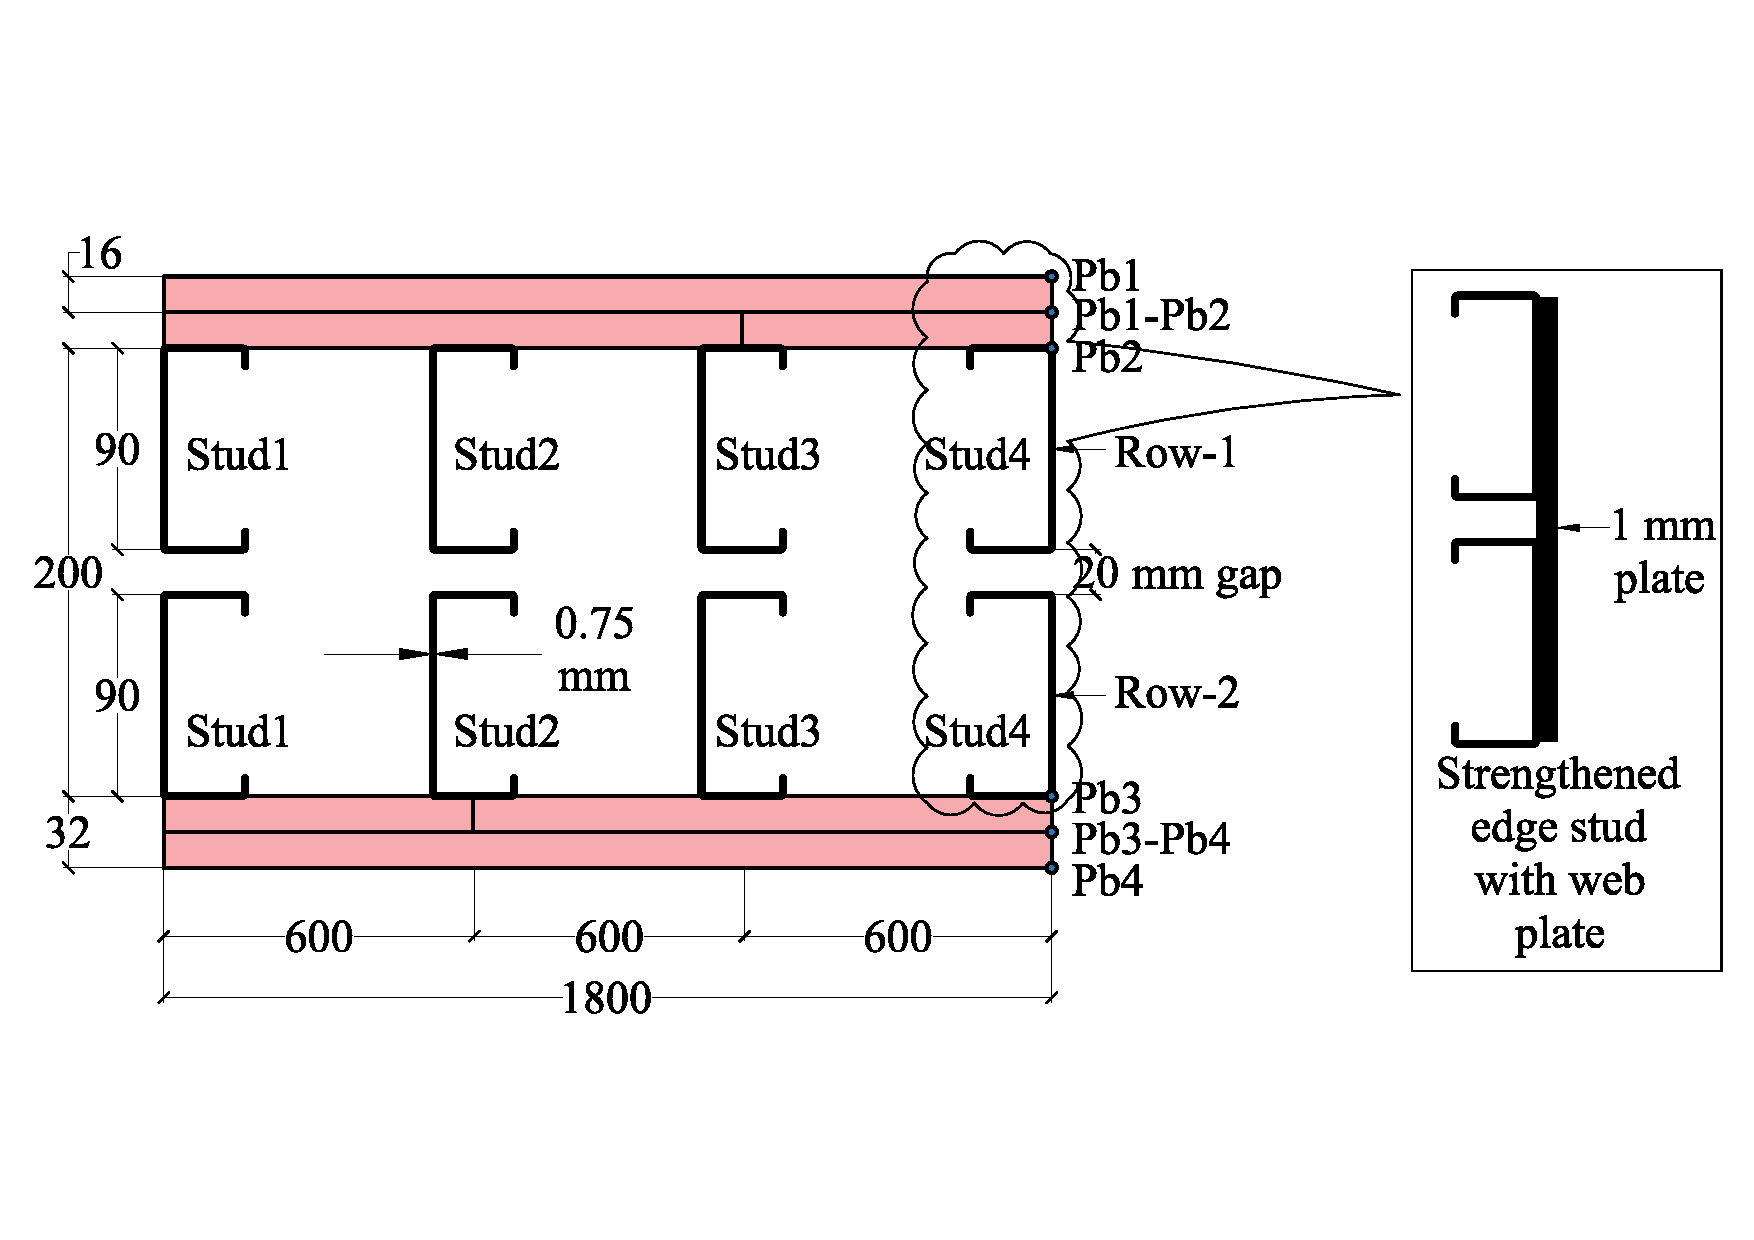
\includegraphics[scale=0.25]{AT2-plan.pdf}\\
		\caption{Test-AT2 configuration}
		\label{fig:AT2-plan}
\end{figure}  
\begin{figure}[!htbp]
	\centering
			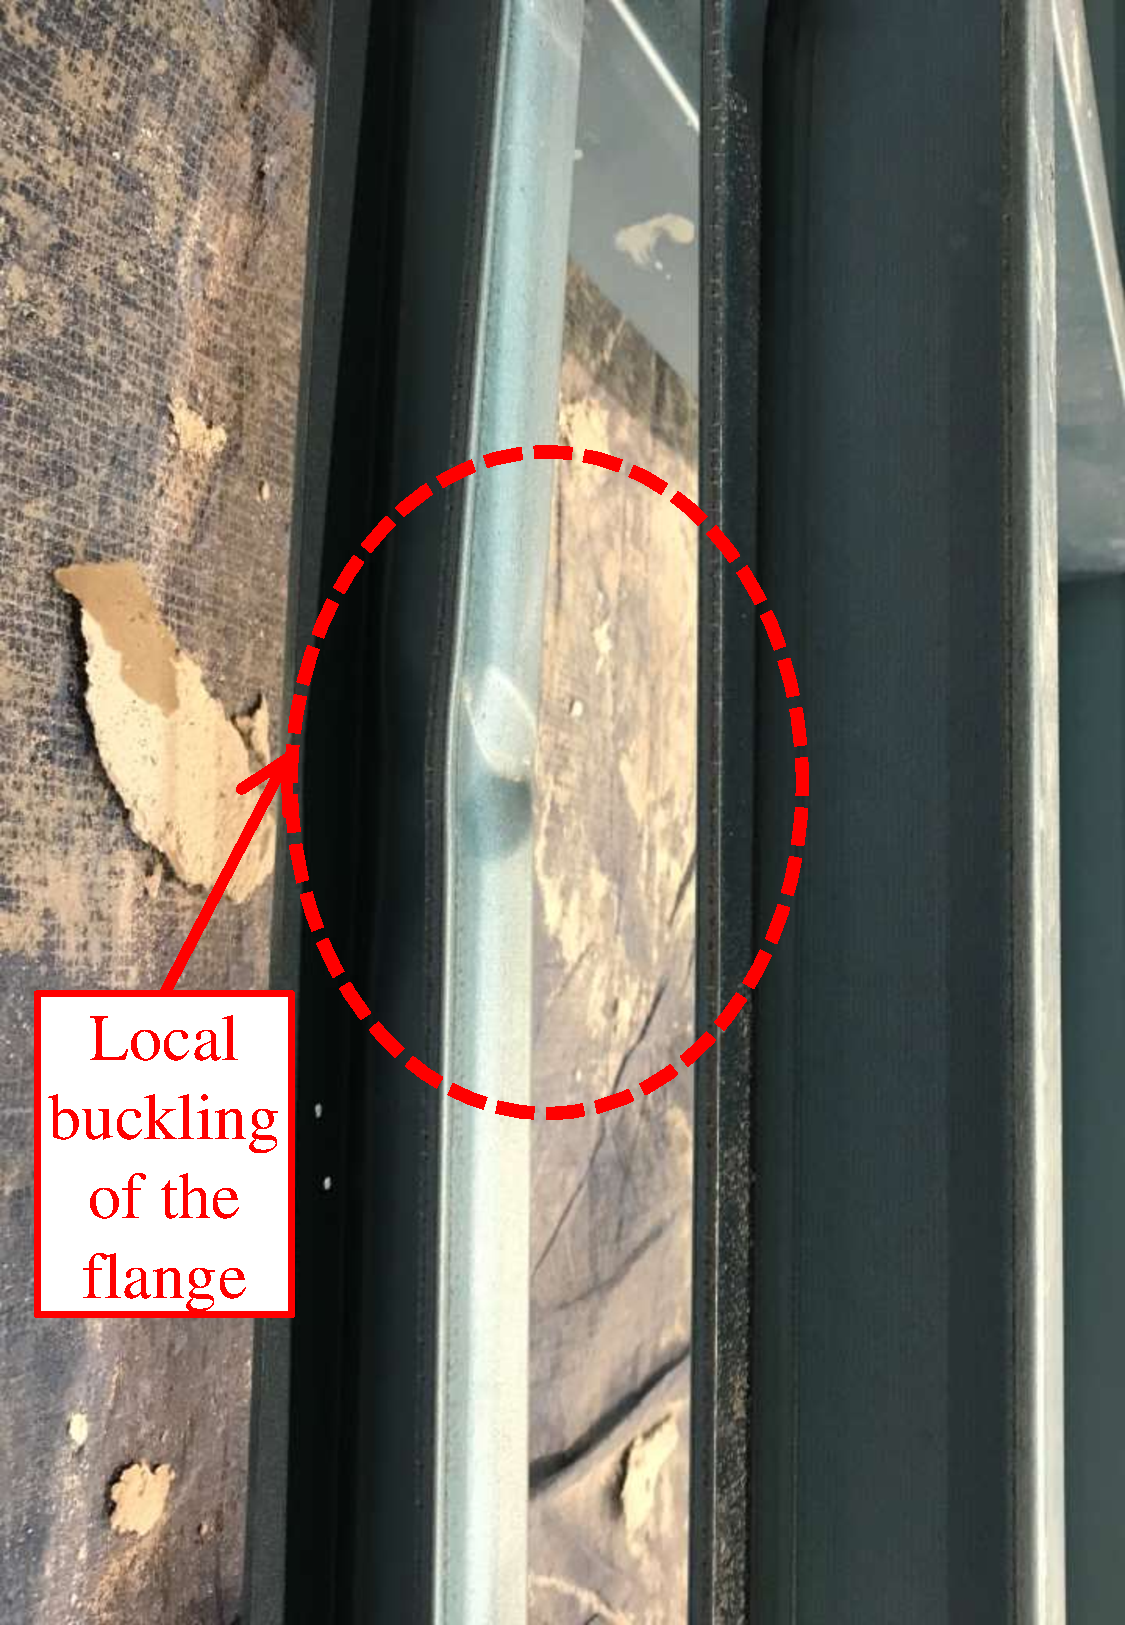
\includegraphics[scale=0.25]{AT2-buckling.pdf}\\
		\caption{Local compressive failure in test-AT2}
		\label{fig:AT2-buckling}
\end{figure}
\begin{figure}
	\centering
		\begin{tabular}{cc}
			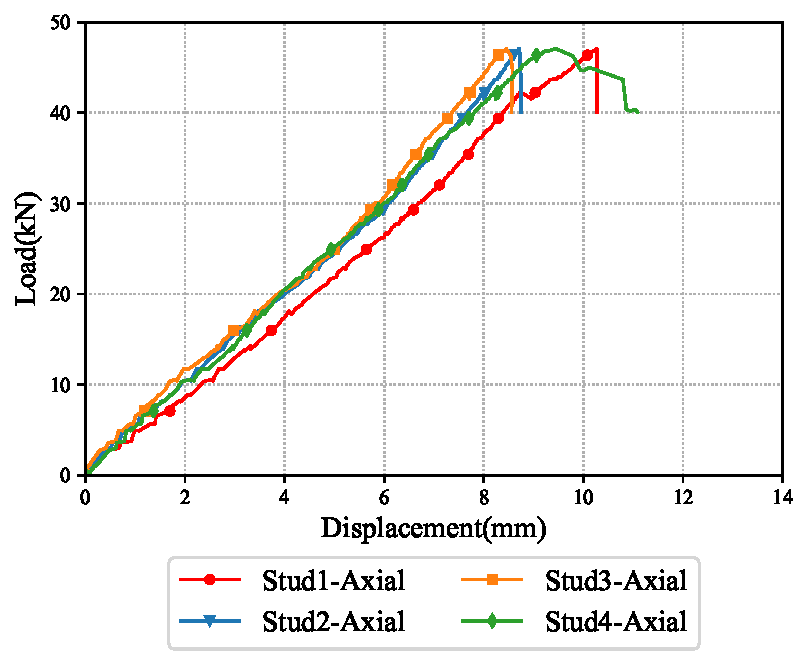
\includegraphics[width=6.5cm,height=6cm]{AT2-Load-Axial-Corrected.pdf} & 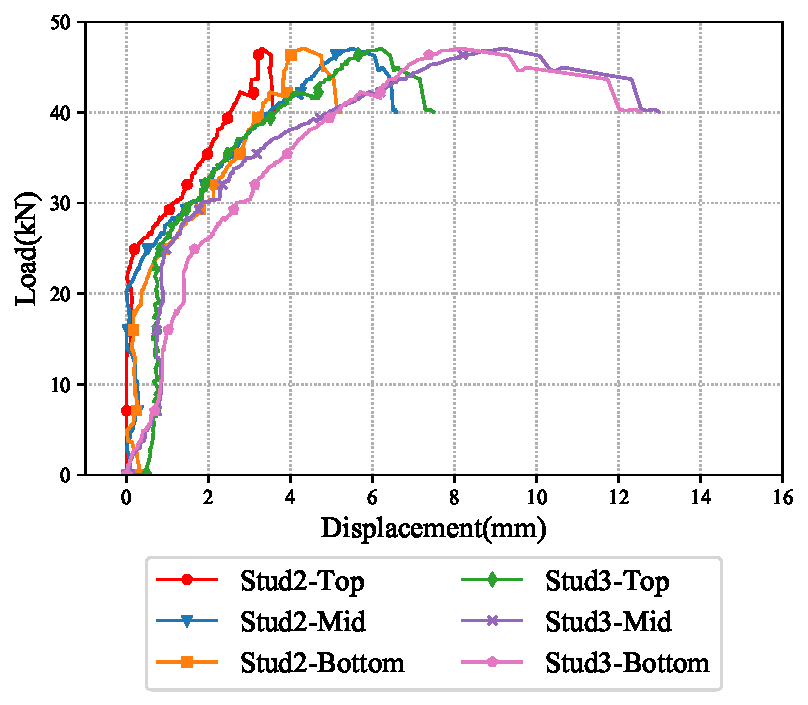
\includegraphics[width=6.5cm,height=6cm]{AT2-Load-Lateral-Corrected.pdf} \\ 
			(a) & (b)  \\ 
		\end{tabular} 
		\caption{Test-AT2 results - (a) Axial displacement and (b) Lateral deflection versus applied axial load}
		\label{fig:AT2-results}
\end{figure}
Figures~\ref{fig:AT2-results}~(a)~and~(b) shows the axial displacement and lateral deflection curves from the ambient capacity Test-AT2. The maximum axial displacement recorded was 10.27 mm in all tests as shown in \Cref{fig:AT2-results}~(a). However, as explained in the previous Test-AT1, the corner stud experience post buckling load resulting in an axial displacement of 16.51 mm. A lateral deflection of 25.18 mm at Stud3-Bottom was recorded as shown in \Cref{fig:AT2-results}~(b). The deflections are more in comparison with Test-AT1. This is because of thin stud section used in this test which has a higher slenderness ratio in comparison with Test-AT1.

\section{Ambient Test-AT3}

The third ambient capacity test was similar to Test-AT2 but with six studs. This test was conducted with six studs to verify the axial compression capacity of double studs LSF wall Test-AT2. \Cref{fig:AT3-plan} shows the test configuration of double stud LSF wall tested with six studs. It is to note that, despite having six studs in the test wall the effective in-plane restraints provided by the plasterboards is applicable only to four studs in the middle leaving the end two studs with partial restraint. This is because the effective distance between the middle two studs are 300 mm on either sides while the effective distance in only 300 mm on one side for the end studs. Similar to the previous ambient capacity tests, after the initial pre-loading cycle, the ambient capacity of the test wall was determined by applying axial compressive load to the individual studs. The test wall resulted in a maximum axial compression capacity of 39.42 kN. Local bearing failure was observed in the end stud as shown in \Cref{fig:AT3-buckling}.
\begin{figure}[!htbp]
	\centering
			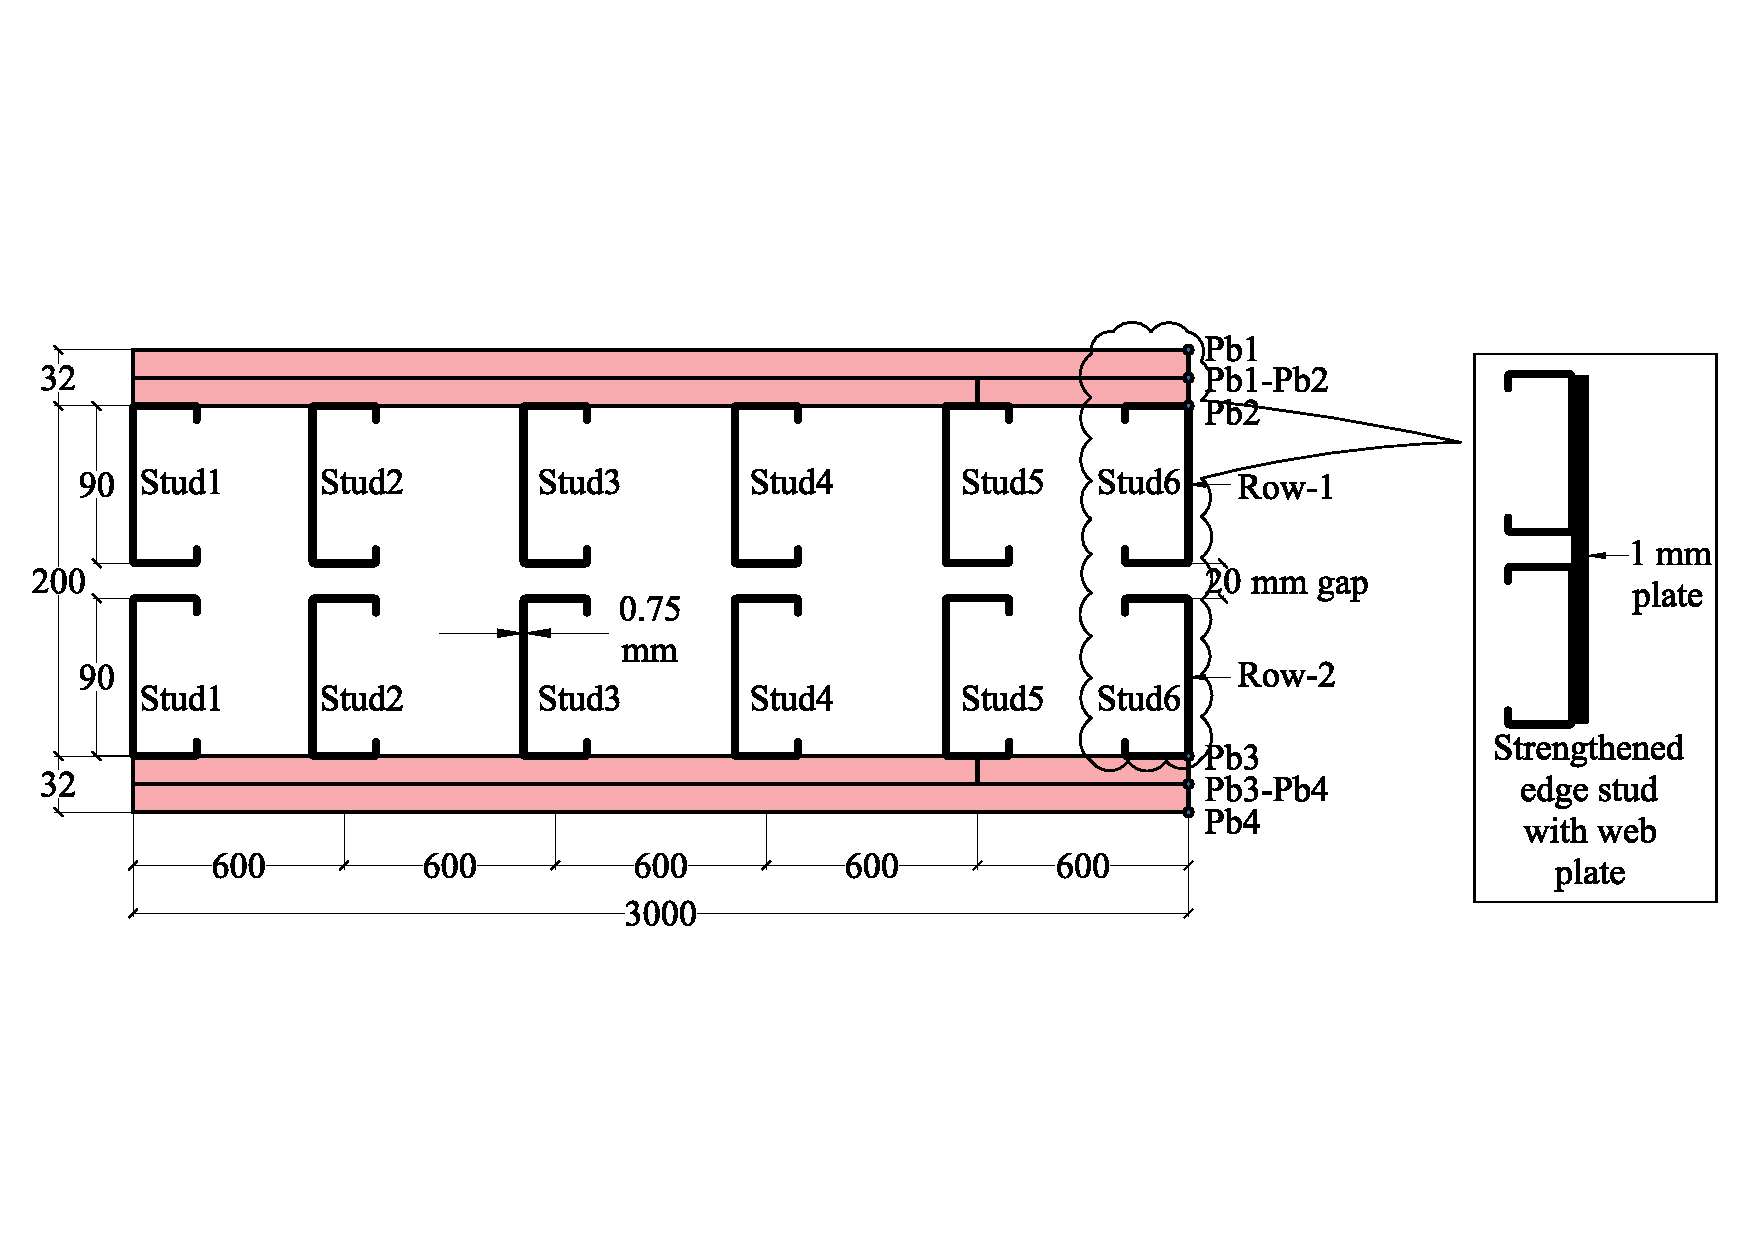
\includegraphics[scale=0.25]{AT3-plan.pdf}\\
		\caption{Test-AT3 configuration}
		\label{fig:AT3-plan}
\end{figure}  
\begin{figure}[!htbp]
	\centering
			\includegraphics[scale=0.3]{AT3-buckling.pdf}\\
		\caption{Local bearing failure in test-AT3}
		\label{fig:AT3-buckling}
\end{figure}

The axial displacement and lateral deflection curves are presented in \Cref{fig:AT3-results} (a)~and~(b). Maximum axial displacement of 9 mm was recorded in Stud2 and a maximum lateral deflection of 6.41 mm was observed at Stud4-Bottom. In comparison with Test-AT2 the axial compression capacity was 7.66 kN lesser. This was due to the bearing failure experienced in the end studs in comparison to local buckling failure in Test-AT2. The plasterboards do not provide effective lateral restraints to the end studs in comparison to the middle studs causing this failure. However, the axial displacement and lateral deflections were similar both Tests-AT2 and AT3 but for the end studs as shown in \Cref{fig:AT3-results}~(a). 
\begin{figure}[!htbp]
	\centering
		\begin{tabular}{cc}
			\includegraphics[width=6.5cm,height=6cm]{AT3-Load-Axial-Corrected.pdf} & \includegraphics[width=6.5cm,height=6cm]{AT3-Load-Lateral-Corrected.pdf} \\ 
			(a) & (b)  \\ 
		\end{tabular} 
		\caption{Test-AT3 results - (a) Axial displacement and (b) Lateral deflection versus applied axial load}
		\label{fig:AT3-results}
\end{figure}

\section{Ambient Test-AT4}

The ambient Test-T4 was conducted on double stud LSF wall with 70 mm stud depth. The stud dimensions were 70\(\times\)29.5\(\times\)8\(\times\)0.95 mm. This test was conducted to investigate the ambient load carrying capacity of double stud LSF walls with 70 mm studs. Four studs were used for the ambient capacity test and the test configuration is show in \Cref{fig:AT4-plan}. After the initial preloading sequence, axial load was applied in increments to determine the axial compression capacity of the test wall. The test wall resulted in an axial compression load of 86.21 kN at the end of the test. Significant local buckling in Stud3 web and flanges was observed in the test wall post test observation as shown in \Cref{fig:AT4-failure}~(b). The buckling failure was noticeable on one Stud3 in row one only. A large crack on the ambient side plasterboard was also observed at the stud failure location as shown in \Cref{fig:AT4-failure}~(a).
\begin{figure}[!htbp]
	\centering
			\includegraphics[scale=0.25]{AT4-plan.pdf}\\
		\caption{Test-AT4 configuration}
		\label{fig:AT4-plan}
\end{figure}  
\begin{figure}[!htbp]
	\centering
		\begin{tabular}{cc}
			\includegraphics[scale=0.2]{AT4-plasterboard_crack.pdf} & \includegraphics[scale=0.2]{AT4-buckling.pdf} \\ 
			(a) & (b)  \\ 
		\end{tabular} 
		\caption{Test-AT4 results - (a) Plasterboard crack and (b) Buckling of stud}
		\label{fig:AT4-failure}
\end{figure}

The axial displacement and lateral deflection curves of Test-AT4 are shown in \Cref{fig:AT4-results} (a)~and~(b). Maximum axial compression of 31.65 mm was recorded at the LVDT measured at Stud3. This indicates the structural failure on Stud3 as witnessed in \Cref{fig:AT4-failure}~(b). The maximum lateral deflection was 16.77 mm at Stud2-Mid (1500 mm) indicating the out-of plane deflection in the test wall. Comparison with the ambient capacity Test-T1 revealed that the axial compression capacity resulted as a part of this test was higher in comparison with the former. This increase in axial compression capacity has been attributed by several factors such as the geometric dimensions of the studs used in Test-T4. Also, the slenderness ratio (b/t) of the studs used in Test-T1 is 93.68 while it is 71.57 for Test-T3 if the local buckling of the web is considered. Based on the aforesaid criteria the studs used in Test-T1 are more slender in comparison with Test-T4 resulting in an increased axial compression capacity in Test-T3. 
\begin{figure}
	\centering
		\begin{tabular}{cc}
			\includegraphics[width=6.5cm,height=6cm]{AT4-Load-Axial-Corrected.pdf} & \includegraphics[width=6.5cm,height=6cm]{AT4-Load-Lateral-Corrected.pdf} \\ 
			(a) & (b)  \\ 
		\end{tabular} 
		\caption{Test-AT4 results - (a) Axial displacement and (b) Lateral deflection versus applied axial load}
		\label{fig:AT4-results}
\end{figure}

\section{Ambient Test-AT5}

The last ambient capacity test in the test series was conducted on a staggered stud LSF wall. The configuration of the wall used in this test is distinctive in comparison with other ambient tests. The test wall consisted of two rows of studs positioned in a staggered manner. LCS were used as studs with dimensions measuring 90\(\times\)36\(\times\)7\(\times\)0.95 mm. Total of eleven studs were used in a staggered configuration as shown in \Cref{fig:AT5-plan}. All the ambient capacity tests (AT1-AT4) had UCS noggings connecting the flanges and provide in-plane lateral restraint at 1 m intervals. However, in staggered stud wall the discontinuity between the stud rows are necessary to achieve the required acoustic rating. Therefore, omega noggings were used at 1 m intervals to provide in-plane lateral restraints to the studs under axial compression. The omega noggings are connected to every alternate studs on the stud webs at service holes through a connecting clip. The clips are held on to web at one end and snapped on to the groves of the omega nogging at two locations. The nogging to stud connection details are shown in \Cref{fig:AT5-construction}~(a). End cleats were used to connect the unrestrained stud flanges to the track to facilitate fixity conditions in the ambient capacity test as shown in \Cref{fig:AT5-construction}~(b). 
\begin{figure}[!htbp]
	\centering
			\includegraphics[scale=0.25]{AT5-plan.pdf}\\
		\caption{Test-AT5 configuration}
		\label{fig:AT5-plan}
\end{figure}
\begin{figure}[!htbp]
	\centering
		\begin{tabular}{cc}
			\includegraphics[width=4cm,height=5.5cm]{omega_connection.pdf} & \includegraphics[width=8cm,height=5.5cm]{AT5-construction.pdf} \\ 
			(a) & (b)  \\ 
		\end{tabular} 
		\caption{Test-AT5 - (a) Omega nogging and clip connection (b) Staggered stud wall construction}
		\label{fig:AT5-construction}
\end{figure}
\begin{figure}[!htbp]
	\centering
		\begin{tabular}{cc}
			\includegraphics[width=5.5cm,height=8cm]{AT5-plasterboard.pdf} & \includegraphics[width=5.5cm,height=8cm]{AT5-buckling.pdf} \\ 
			(a) & (b)  \\ 
		\end{tabular} 
		\caption{Test-AT5 - failure (a) Plasterboard open up and (b) Buckling of studs}
		\label{fig:AT5-failure}
\end{figure}
\begin{figure}
	\centering
		\begin{tabular}{cc}
			\includegraphics[width=6.5cm,height=6cm]{AT5-Load-Axial-Corrected.pdf} & \includegraphics[width=6.5cm,height=6cm]{AT5-Load-Lateral-Corrected.pdf} \\ 
			(a) & (b)  \\ 
		\end{tabular} 
		\caption{Test-AT5 results - (a) Axial displacement and (b) Lateral deflection versus applied axial load}
		\label{fig:AT4-results}
\end{figure}

The test wall was loaded through a 20 mm thick base plate connecting the rams and the axial compression load was applied individually to the staggered studs. The end studs of the test wall were strengthened as the plasterboards do not provide effective lateral restraints to the end studs as discussed in \Cref{sec:AT1}. After the application of initial preload the ambient capacity test was conducted by gradual increase in the applied axial load till failure. The test wall resulted an axial compression capacity of 68.49 kN. A maximum axial displacement of 21.62 mm was recorded in Stud3 at the end of the test. The maximum lateral deflection of 13 mm was recorded at 750 mm from the bottom of the specimen near Stud4. Plasterboard open up was noticeable near the stud failure locations as shown in \Cref{fig:AT5-failure}~(a). Local buckling of the web and flanges were observed post test investigation as shown in \Cref{fig:AT5-failure}~(b).

\section{Summary of Ambient Capacity Tests}

The summary of all the ambient capacity tests conducted on double and staggered stud LSF walls are presented and discussed in this section. A total of five ambient capacity tests were conducted and the results are summarised in the \Cref{tab:ambient-test-results}. The axial compression capacity of 90 mm and 70 mm wide studs with various thicknesses and stud configurations were considered for the investigation. Ambient tests AT1 to AT4 were conducted on double stud walls with 90 mm and 70 mm wide studs. The cavity depth of the test wall was 200 mm for Tests-AT1 to AT3 while it was 160 mm for Test-AT4. Thickness of the studs were 0.95 mm for Tests-AT1 and AT4 while the thickness was 0.75 mm for Test-AT2 and AT3. Test-AT5 was conducted on staggered stud LSF wall comprising of 90 mm studs with a cavity depth of 150 mm and a stud thickness of 0.95 mm.  
\begin{table}[!htbp]
	\centering
	\caption{Ambient test panel details - Summary}
	\begin{tabular}{ccccccc}
		\toprule
		\multicolumn{1}{m{2.4em}}{\centering{Test Name}} & 
		\multicolumn{1}{m{5.6em}}{\centering{Description}} & 
		\multicolumn{1}{m{2.85em}}{\centering{Stud Depth (mm)}} & 
		\multicolumn{1}{m{2.85em}}{\centering{Cavity Depth (mm)}} & 
		\multicolumn{1}{m{5em}}{\centering{Stud Thickness (mm)}} & 
		\multicolumn{1}{m{3em}}{\centering{No of Studs}} &
		\multicolumn{1}{m{3em}}{\centering{Failure Load (kN)}} \\
		\midrule
		AT1  & Double Stud & 90 & 200 & 0.95 & 4 & 73 \\
		AT2  & Double Stud & 90 & 200 & 0.75 & 4 & 47.08 \\
		AT3  & Double Stud & 90 & 200 & 0.75 & 6 & 39.42 \\
		AT4  & Double Stud & 70 & 160 & 0.95 & 4 & 86.21 \\
		AT5  & Staggered Stud & 90 & 200 & 0.95 & 6 & 68.49 \\
		\bottomrule
	\end{tabular}%
	\label{tab:ambient-test-results}%
\end{table}%

The double stud wall Test-AT1 with 0.95 mm thick 90 mm wide studs resulted in an axial compression capacity of 73 kN while Test-AT4 which had the same stud thickness and 70 mm wide studs resulted in an axial compression capacity of 86 kN. This is 13 kN higher in comparison with Test-AT1. The reduction in axial compression capacity is attributed by the higher slenderness ratio of the studs in Test-AT1 due to the geometric profile. The Tests-AT2 and AT3 resulted in an axial compression capacity of 47.08 and 39.42 kN. Despite the same testing configuration and stud thickness the number of studs were only varied. The variation in axial compression capacity was due to the absence of effective plasterboard restraints to the end studs resulting in bearing failure at supports. However, the difference in axial compression capacity between the Tests-AT2 and AT is small and can be ignored. The staggered stud wall Test-AT5 resulted in an axial compression capacity of 68.49 kN which is comparatively closer to Test-AT1 with the same stud depth and thickness. However, the arrangement of studs were different in both the tests. In Test-T1 the test wall had the stud rows in a linear pattern while in Test-T5 the studs were staggered. The effective centre-to-centre distance between the studs were 600 mm in the double stud wall Test-T1 while it was 300 mm in the staggered stud wall Test-AT5. But it is to note that the cavity depth of Test-AT1 was 200 mm while it was 150 mm for Test-AT5 which is beneficial in reducing effective floor space in LSF wall construction.

\section{Comparison of Ambient Capacity Test Results}

As the ambient capacity tests were conducted for two different configurations, it becomes a necessity to compare the test results to determine a better understanding about the axial compression behaviour of these complex LSF walls under ambient conditions. Also Test-T1 to T4 were conducted using LCS noggings while Test-T5 was conducted with omega noggings. This adds to the novelty of the ambient capacity tests. The stud flanges in single stud walls are effectively restrained by plasterboard on both sides while in complex LSF walls the effective restraints provided by the plasterboard is limited to one flange only. Therefore, comparisons are made against ambient capacity test results from single stud wall with 92 mm studs and 150 mm studs to understand the difference in axial compression behaviour of the complex LSF walls. Test results used for the comparison are detailed in \Cref{tab:ambient-test-results-comparison}. Comparisons with the 90 mm single stud are made against tow thicknesses 0.75 and 1.15, while for 150 mm single studs the comparisons are made against 1.15 mm thickness only. This is due to the limited availability of the ambient capacity test results. Single stud tests were conducted previously at QUT Wind and Fire Engineering Laboratory. Further details about Test-S-AT2 can be found in \citet{Gunalan2013e}, while for Test-S-T1 and S-T2 details are available as internal reports. 
\begin{table}[!htbp]
	\centering
	\caption{Ambient test panel details - Summary}
	\begin{tabular}{ccccccc}
		\toprule
		\multicolumn{1}{m{2.4em}}{\centering{Test Name}} & 
		\multicolumn{1}{m{5.6em}}{\centering{Description}} & 
		\multicolumn{1}{m{2.85em}}{\centering{Stud Depth (mm)}} & 
		\multicolumn{1}{m{2.85em}}{\centering{Cavity Depth (mm)}} & 
		\multicolumn{1}{m{5em}}{\centering{Stud Thickness (mm)}} & 
		\multicolumn{1}{m{3em}}{\centering{No of Studs}} &
		\multicolumn{1}{m{3em}}{\centering{Failure Load (kN)}} \\
		\midrule
		AT1  & Double Stud & 90 & 200 & 0.95 & 4 & 73 \\
		AT2  & Double Stud & 90 & 200 & 0.75 & 4 & 47.08 \\
		AT4  & Double Stud & 70 & 160 & 0.95 & 4 & 86.21 \\
		AT5  & Staggered Stud & 90 & 150 & 0.95 & 11 & 68.49 \\
		S-AT1 & Single Stud & 90 & 90 & 0.75 & 2 & 33.10 \\
		S-AT2 & Single Stud & 90 & 90 & 1.15 & 4 & 79.24 \\
		S-AT3 & Single Stud & 150 & 150 & 1.15 & 6 & 45.43 \\
		\bottomrule
	\end{tabular}%
	\label{tab:ambient-test-results-comparison}%
\end{table}%

Firstly comparisons were made against 90 mm studs on single and double stud LSF walls. This include stud thickness of 0.75, 0.95 and 1.15 mm. Secondly, comparisons were made against staggered stud and single stud wall with 150 mm cavity depth. The stud thickness used in staggered stud wall was 0.95 mm with 90 mm stud depth while for single stud wall 150 mm deep studs with 1.15 mm thickness were used. Also, the 70 mm stud double stud wall Test-AT4 was also compared to understand the axial compression capacity of the single and double stud walls under different plasterboard restraint conditions. Comparisons are made against the maximum axial load carrying capacity. Variations in effective restraints provided by plasterboards for different configurations are also discussed and their effect on the axial load carrying capacity was also investigated. Applied load versus axial displacement is compared against single and double stud walls with 90 and 150 mm cavity depth and are shown in \Cref{fig:90mm-comparison-ambient,fig:150mm-comparison-ambient}.
\begin{figure}[!htbp]
	\centering
			\includegraphics[width=10cm,height=9cm]{90mm-Axial-comparison.pdf}\\
		\caption{Tensile coupon details}
		\label{fig:90mm-comparison-ambient}
\end{figure}
\begin{figure}[!htbp]
	\centering
			\includegraphics[width=10cm,height=9cm]{150mm-Axial-comparison.pdf}\\
		\caption{Tensile coupon details}
		\label{fig:150mm-comparison-ambient}
\end{figure}

Maximum axial compression capacity was recorded in single stud wall with stud thickness of 1.15 mm (S-AT2) resulting in a failure load of 79.24 kN. The least axial compression capacity was recorded in single stud wall with 0.75 mm stud (S-AT1) resulting in a failure load of 33.10 kN. In single stud LSF walls, the plasterboards provide effective lateral restraints preventing the in plane buckling of studs. As the studs locally buckle, the out of plane plasterboard restraint is not generally critical under ambient conditions. However, in the case of single stud wall with 150 mm studs the axial compression capacity was 45.43 kN which is 33.81 kN lesser than the corresponding single stud wall with 90 mm studs. This is attributed by the wider web depth in 150 mm studs resulting in lesser axial compression capacity.

In case of double stud LSF walls the effective plasterboards restraints are provided to one flange only on each stud rows. The inner stud flanges in the LSF wall are restrained at 1 m intervals through noggings. This results in inadequate in-plane plasterboard restraints to the studs resulting in reduced axial compression capacity. If the double stud wall Test-AT1 is taken for consideration, an axial compression capacity of 73 kN was recorded for both the stud rows. This attributes to 36.5 kN per stud which is 42.74 kN less than single stud wall Test-S-AT1 with 90 mm studs restrained on both the flanges. However, it is to note that the double stud wall was tested with a stud thickness of 0.95 mm while the single stud wall had a stud thickness of 1.15 mm. It can be inferred that the thickness of the studs significantly affect the axial compression capacity under ambient conditions. If the single stud wall Test-S-AT1 is compared with the double stud wall Test-AT2, in which the studs thickness was 0.75 mm in both the cases, the axial compression capacity was 23.54 kN per stud (47.08/2) in double stud wall Test-AT2, whereas it was 33.10 kN in single stud wall Test-S-AT1. The reduction in axial compression capacity was 9.56 kN. However, the double stud wall Test-AT4 with 70 mm studs resulted in a higher axial compression capacity of 86.21 kN (86.21/2 = 43.105 kN per stud) in comparison with double stud wall with 90 mm studs (Test-AT1). Despite having the same stud thickness and wall configuration the 70 mm double stud wall resulted in higher axial compression capacity. This can be attributed to higher slenderness in 90 mm studs in comparison with the 70 mm studs. However, the axial compression capacity of 90 mm single stud LSF wall lined with plasterboard on both sides resulted in a higher compression capacity in comparison with double and staggered stud walls 

Comparing the LSF walls with 150 mm cavity depth, the axial compression capacity was 68.49 kN in staggered stud wall Test-AT5 and 45.43 kN in 150 mm single stud wall Test-S-AT3. This is a significant reduction in the axial compression capacity. It is to note that the stud spacing was staggered with an effective spacing of 300 mm in staggered stud wall Test-AT5 while the stud spacing was maintained at 600 mm in 150 mm wide single stud wall Test-S-AT3. Also, the omega noggings were connected through the stud webs while no nogging restraints were provided for Test-S-AT3. Despite having a higher stud thickness of 1.15 mm the 150 mm wall Test-S-AT3 resulted in a reduced axial compression capacity. 

\section{Tensile Coupon Tests}

Tensile coupon tests were conducted to determine the Young's Modulus and yield strength of the steel studs in LSF wall, later to be used for numerical analysis. Details of the coupon specimen is given in \Cref{fig:tensile-coupon-details}. Coupons were cut on the web and flanges of the studs at three locations along the 3 m long studs to arrive at the weighted average values of yield strength. The tensile coupon tests were conducted using Instron machine which operates on Bluehill software. Extensometers were used to measure the rate of elongation during the test through which corresponding strain was computed. Detail view of specimen used for the tensile coupon test is shown in \Cref{fig:tensile-coupon-details}.  
\begin{figure}[!htbp]
	\centering
			\includegraphics[scale=0.4]{tensile-coupon-details}\\
		\caption{Tensile coupon details}
		\label{fig:tensile-coupon-details}
\end{figure}
\begin{figure}[!htbp]
	\centering
			\includegraphics[width=4cm,height=6cm]{Coupon-test-setup.pdf}\\
		\caption{Tensile coupon details}
		\label{fig:tensile-coupon-test-setup}
\end{figure}
% Table generated by Excel2LaTeX from sheet '0.75'
\begin{table}[htbp]
	\centering
	\caption{Tensile coupon test results for 0.75 mm thick studs}
	  \begin{tabular}{cccc}
	  \toprule
	  \multicolumn{1}{p{2.145em}}{\centering Test\newline{}No} & 
	  \multicolumn{1}{p{4.07em}}{\centering Sample\newline{}Location} & 
	  \multicolumn{1}{p{7.07em}}{\centering Youngs\newline{}Modulus (Gpa)} & 
	  \multicolumn{1}{p{7.145em}}{\centering Yield\newline{}Strength (Mpa)} \\
	  \midrule
	  1    & Web  &  202.55 & 634.39 \\
	  2    & Web  &  232.30 & 658.45 \\
	  3    & Web  &  220.46 & 633.09 \\
	  4    & Web  &  214.28 & 642.87 \\
	  5    & Web  &  218.17 & 643.57 \\
	  6    & Web  &  212.95 & 642.92 \\
	  7    & Flange &  212.43 & 648.66 \\
	  8    & Flange &  216.45 & 658.30 \\
	  9    & Flange &  217.55 & 660.50 \\
	  \midrule
	  \multicolumn{2}{c}{Average} & 216.35 & 646.97 \\
	  \bottomrule
	  \end{tabular}%
	\label{tab:075-coupon-results}%
  \end{table}%
  % Table generated by Excel2LaTeX from sheet '0.95'

  \begin{table}[htbp]
	\centering
	\caption{Tensile coupon test results for 0.95 mm thick studs}
	  \begin{tabular}{ccccc}
	  \toprule
	  \multicolumn{1}{p{2.145em}}{\centering Test\newline{}No} & 
	  \multicolumn{1}{p{4.07em}}{\centering Sample\newline{}Location} & 
	  \multicolumn{1}{p{7.07em}}{\centering Youngs\newline{}Modulus (Gpa)} & 
	  \multicolumn{1}{p{7.145em}}{\centering Yield\newline{}Strength (Mpa)} \\
	  \midrule
	  10   & Web  &  216.50 & 612.88 \\
	  11   & Web  &  219.12 & 623.75 \\
	  12   & Web  &  202.83 & 622.87 \\
	  13   & Flange &  217.91 & 620.68 \\
	  14   & Flange &  218.56 & 620.56 \\
	  15   & Flange &  218.35 & 604.45 \\
	  \midrule
	  \multicolumn{2}{c}{Average} & 215.55 & 617.53 \\
	  \bottomrule
	  \end{tabular}%
	\label{tab:095-coupon-results}%
  \end{table}%

Tensile coupon test set up is shown in \Cref{fig:tensile-coupon-test-setup}. Details of the tensile coupon testes are presented in \Cref{tab:075-coupon-results,tab:095-coupon-results}. Total of 15 tensile coupon tests were conducted to determine the Young's Modulus and yield strength of the steel used in the ambient capacity tests. The average Young's Modulus and yield strength of 0.75 mm thick studs were 216.35 GPa and 646.97 MPa respectively. Likewise, for 0.95 mm thick steel, the average Young's Modulus and yield strength were 215.55 GPa and 617.53 MPa respectively. The yield strength of 0.75 mm thick steel was higher in comparison with 0.95 mm steel. Tensile coupons were extracted only from the stud web and flanges as these elements are most susceptible to internal stresses during the cold forming process. Tests were not conducted on the noggings and tracks as they are least susceptible to internal stresses and are not considered for the purpose of design and numerical analysis. The stress-strain curve corresponding to the specimens with the maximum Young's modulus and yield strength recorded in the web and flanges of 0.75 mm and 0.95 mm steel are shown in \Cref{fig:075-stress-strain,fig:095-stress-strain} below.
\begin{figure}
	\centering
		\begin{tabular}{cc}
			\includegraphics[width=6.5cm,height=5.5cm]{Test2-Specimen_RawData_5.pdf} & \includegraphics[width=6.5cm,height=5.5cm]{Test9-Specimen_RawData_4.pdf} \\ 
			(a) & (b)  \\ 
		\end{tabular} 
		\caption{Stress-strain curve from tensile coupon tests on 0.75 mm steel (a) Stud Web (b) Stud Flange}
		\label{fig:075-stress-strain}
\end{figure}
\begin{figure}
	\centering
		\begin{tabular}{cc}
			\includegraphics[width=6.5cm,height=5.5cm]{Test11-Specimen_RawData_6.pdf} & \includegraphics[width=6.5cm,height=5.5cm]{Test13-Specimen_RawData_8.pdf} \\ 
			(a) & (b)  \\ 
		\end{tabular} 
		\caption{Stress-strain curve from tensile coupon tests on 0.95 mm steel (a) Stud Web (b) Stud Flange}
		\label{fig:095-stress-strain}
\end{figure}

\section{Summary of Ambient Capacity Tests Investigations and Comparisons}

The following findings can be drawn from ambient capacity tests on single, double and staggered stud LSF walls and tensile coupon tests.
\begin{itemize}
	\item Axial compression capacity is greatly dependant on the thickness and depth of the studs.
	\item The effect of plasterboards on the stud flanges providing in-plane restraints significantly influences the axial compression capacity in single stud LSF walls. The absence of effective plasterboard restraints on the inner stud flanges in double stud walls greatly affects the axial compression capacity of double stud LSF walls.
	\item In the case of staggered stud LSF walls, despite the absence of plasterboard restraint on one flange, the omega noggings connecting the stud webs provide significant in-plane restraints to the studs resulting in a similar axial compression capacity in comparison with double stud LSF walls.
	\item The axial compression capacity of plasterboard line double stud walls are significantly higher for walls with 70 mm studs in comparison with 90 mm studs with the same thickness. This is attributed by the increased slenderness in 90 mm studs. 
	\item All the tensile coupon tests show that the minimum guaranteed yield strength of 550 MPa is achieved in all the test specimens. 0.75 mm steel resulted in higher yield strength in comparison with 0.95 mm steel despite the same grade of steel. However, the Young's Modulus remains almost similar irrespective of the thickness. This is because of the higher cold work in steel with lower thicknesses. The Young's Modulus and yield strength results from the coupon tests will later be used for numerical analysis. 
\end{itemize}
  
  
  
 

\chapter{Experimental Investigations under Fire Conditions}
\label{ch:Fire}       
\section{General}
This chapter details the experimental investigations conducted on complex LSF wall systems. To determine the fire performance of LSF wall systems fire tests are still the preferred method and are generally accurate. Therefore, extensive experimental investigations were carried out on a series of complex LSF walls under load bearing and non-load bearing conditions. The ambient capacity test results from \Cref{ch:Ambient} is used to apply the appropriate loads for the fire test discussed in this chapter.

\section{Heat Transfer in LSF Walls}

In single stud LSF walls exposed to fire on one side the heat transfer happens by conduction through plasterboards from fire side to ambient side. This is followed by convection and radiation within the cavity. Conduction and radiation through the studs also contribute significantly to the heat transfer across the wall. In single stud walls the plasterboards provide intermittent lateral restraints to both flanges of the stud depending on the screw locations and protects the steel studs during fire. The fire resistance level is greatly influenced by the number of plasterboard layers used \citet{Kodur2006,Ariyanayagam2016}. Generally, in a single stud wall with two layers of plasterboard lining the fire exposed plasterboard transfers the heat to the subsequent plasterboard layer and reaches the stud hot flange through conduction. But within the cavity, the heat transfer from fire side cavity surface to the ambient side cavity surface occurs through both convection and radiation. Air within the cavity offers certain resistance to the heat transfer depending upon the depth and volume of the air cavity.  There is also a certain amount of heat transfer through the conduction of air within the cavity. But the conductivity of air is low when compared to plasterboard at higher temperatures. There is also a significant amount of radiation into the cavity and conduction through the studs in single stud walls. 

In double stud walls, the heat transfer mechanism from fire side to ambient side is not well understood. The air gap between the two rows of stud reduces the heat transfer through conduction from fire side to ambient side cavity. This results in lower temperatures on the ambient side plasterboard. This can reduce the temperatures across the wall resulting in uniform temperature distribution in the studs. Such reduced temperature gradient can result in reduced thermal bowing and neutral axis shift in comparison with single stud LSF walls. During the fire exposure on one side, the plasterboard on the fire side calcinates at 140\degree C, which is the first dehydration point \citet{Keerthan2012a}. The temperature distribution on the stud will be non-uniform causing thermal bowing. This also leads to non-uniform mechanical properties of steel, resulting in neutral axis shift for studs. These actions caused by fire exposure on one side induce the thin-walled studs to be subjected to a bending moment in addition to the applied axial compression load \citet{Gunalan2013e}. But there is lack of research data to fully understand these effects in double stud walls. Therefore, this research investigated the structural fire performance of three load bearing double stud LSF walls using full scale standard fire tests.

\section{Small-Scale Fire Test on Double Stud LSF Walls}

To investigate the fire performance of complex LSF walls and determine the thermal behaviour, a small-scale fire test was conducted on double stud LSF wall. Small-scale fire tests were considered as pilot study to determine the thermal performance of LSF walls by past researchers. The results from small-scale fire tests are valuable to predict the thermal behaviour of LSF walls through full-scale fire tests before hand. However, only the insulation and integrity failure criteria can be determined using small-scale fire test. Structural failure criteria could be determined only through full-scale fire test for an LSF wall configuration.

\subsection{Small-Scale Fire Test Details}

One small-scale fire test on non-cavity insulated double stud LSF wall was conducted in this research study. The test wall dimensions were 1.2 \(\times\) 1.2 m with an exposed area of 1 \(\times\) 1 m. Propane gas furnace with a single burner was used for the fire test. Two 90 mm studs with 0.95 mm thickness were used for the fire tests. Two layers of 16 mm thick gypsum plasterboard was sheathed on both sides of the test wall panel. Test specimen details are provided in \Cref{fig:ST-setup}(a). K-type thermocouples were used to measure the temperatures across the test wall in various locations during the fire test. The test was conducted under non-load bearing conditions. Therefore the axial and lateral displacements were not measured during the fire test. Apart from the temperature measurements through thermocouples the ambient side temperatures were closely monitored with an infrared gun to witness insulation failure which is one of the critical failure criteria in non-load bearing LSF wall fire tests. 
\begin{figure}[!htbp]
	\centering
		\begin{tabular}{cc}
			\includegraphics[width=7cm,height=6cm]{ST-specimen.pdf} & \includegraphics[width=7cm,height=6cm]{ST-setup.pdf} \\ 
			(a) & (b)  \\ 
		\end{tabular} 
		\caption{Plasterboard and stud time-temperature curves of Test-T1 (a) Average plasterboard temperature (b) Stud3 temperature}
		\label{fig:ST-setup}
\end{figure}
\begin{figure}[!htbp]
	\centering
		\begin{tabular}{cc}
			\includegraphics[width=7cm,height=6cm]{ST-failure1.pdf} & \includegraphics[width=7cm,height=6cm]{ST-failure2.pdf} \\ 
			(a) & (b)  \\ 
		\end{tabular} 
		\caption{Plasterboard and stud time-temperature curves of Test-ST1 (a) Average plasterboard temperature (b) Stud2 temperature}
		\label{fig:ST-failure}
\end{figure}

Test wall was clamped to the small furnace and ceramic insulation was wrapped around the specimen to prevent heat loss around the sides during fire test as shown in \Cref{fig:ST-setup}(b). The test wall was then subjected to AS 1530.4 standard fire curve based on ISO 834 and the fire test was conducted. Mild smoke was noticeable from 30 min till 80 min of the fire test representing the calcination of fire side plasterboard. Also, water droplets were visible on the clamps used for attaching the test wall to the furnace at certain intervals. The fire test was conducted for 176 min after which the test was stopped due to insulation failure criteria where the temperatures on the ambient side at the top left corner exceeded the limiting temperature of 200\degree C. Post fire test investigation revealed severe plasterboard fall-off on fire side resulting in sudden increase in temperature on the ambient side at a particular point. However, the thermocouple measured ambient side plasterboard surface (Pb4) temperatures were well below 100\degree C till the end of fire test. No deformation in the studs were observed as shown in \Cref{fig:ST-failure} as this was a non-load bearing test with shorter stud sections. The plasterboard fall-off was due to the hot air from the furnace concentrated on a small area of the test frame in small-scale fire test for a longer time period.

\subsection{Small-Scale Fire Test - Results and Discussion}

The small-scale fire test results showing the time-temperature evolution of the plasterboards and studs are shown in \Cref{fig:ST1-PB&Stud}(a). Fire side plasterboard interface temperatures (Pb1-Pb2)was flat for the initial 20 min after which a steep rise in the curve was noticed. This was followed by a plateau region from 70 min to 120 min after which the curve increased gradually till the end of fire test. A sudden increase in the time-temperature curves were observed in all the plasterboard surfaces indicating plasterboard fall-off. The possibility of joint open cannot happen as the specimen did not have any plasterboard joints. This unique behaviour in the time-temperature curve is also reflected on the fire side cavity (Pb2) and the ambient side cavity surface (Pb3). However, ambient side plasterboard interface surface (Pb3-Pb4) recorded temperatures less than 100\degree C till 150 min and reaching a maximum of 280\degree at the end of fire test. The stud time-temperature curves are plotted in \Cref{fig:ST1-PB&Stud}(b).  
\begin{figure}[!htbp]
	\centering
		\begin{tabular}{cc}
			\includegraphics[width=7cm,height=6cm]{ST1-Average-Pb.pdf} & \includegraphics[width=7cm,height=6cm]{ST1-Stud1-2-Top.pdf} \\ 
			(a) & (b)  \\ 
		\end{tabular} 
		\caption{Plasterboard and stud time-temperature curves of Test-ST1 (a) Average plasterboard temperature (b) Stud2 temperature}
		\label{fig:ST1-PB&Stud}
\end{figure}

The hot and cold flange temperatures of Stud1 and Stud2 recorded temperatures less than 200\degree C till 65 min of the fire test. A sudden increase in the time-temperature curve of the fire side hot and cold flanges (ST1-Stud1 and Stud2-Top-Fire-HF and CF) was noticed after 65 min, after which the curve exhibits a gradual increase correlating with the corresponding plasterboard temperatures. However the plateau region was not significantly observed in the stud time-temperature curves. The sudden increase in the hot flange temperatures proves the presence of plasterboard fall-off in the fire test. The cold flange temperatures were in close relation with the corresponding hot flange temperatures as shown in \Cref{fig:ST1-PB&Stud}. It is to note that the difference in temperature gradient between the fire the cold flange (ST1-Stud1 and Stud2-Top-Fire-CF) and the ambient side hot and cold flanges (ST1-Stud1 and Stud2-Top-Amb-HF and CF) were small in comparison with the fire side hot and cold flanges. This indicates the delayed heat transfer mechanism in wider cavity LSF walls. This is further investigated and discussed in the full-scale fire test section of this chapter.

\section{Full-scale Fire Test on Double Stud LSF Walls}
\subsection{Fire Test Panel Details}

To investigate the heat transfer mechanism in detail a series of fire tests were conducted on the complex LSF wall system. The test wall panels were constructed with frame dimensions of 3 m \(\times\) 3 m as shown in \Cref{fig:ds-elevation}. Total of 10 full-scale fire tests were conducted for the experimental study. Lipped Channel Sections (LCS) were used as studs and Unlipped Channel Sections (UCS) were used as tracks. Intermittent lateral restraints using 0.55 mm thick noggings located at 1000 mm intervals were provided for some of the fire tests. Stud thickness, cavity depth, load ratio and cavity insulations were the variable parameters and are detailed in \Cref{tab:test-specimens}. G550 steel (minimum yield strength of 550 MPa) was used for all the fire tests.  The studs, tracks and noggings were connected using Buildex M6.0 \(\times\) 15 GX Ca smooth top GA point steel frame and truss screws with studs at 600 mm centres. A 20 mm gap was maintained between the two rows of steel frames by using 50 mm x 200 mm spacer plates. 
\begin{table}[!htbp]
	\begin{threeparttable}
		\centering
			\caption{Fire test panel details}
				\begin{tabular}{ccccccc}
					\toprule
					\multicolumn{1}{m{2.4em}}{\centering{Test Name}} & 
					\multicolumn{1}{m{5.6em}}{\centering{Description}} & 
					\multicolumn{1}{m{2.85em}}{\centering{Stud Depth (mm)}} & 
					\multicolumn{1}{m{2.85em}}{\centering{Cavity Depth (mm)}} & 
					\multicolumn{1}{m{5em}}{\centering{Stud Thickness (mm)}} & 
					\multicolumn{1}{m{5em}}{\centering{Cavity Insulation}} &
					\multicolumn{1}{m{3em}}{\centering{Loading Ratio}}\\
					\midrule
					T1  & Double Stud & 90 & 200 & 0.95 & No & 0.4 \\
					T2  & Double Stud & 90 & 200 & 0.75 & No & 0.4 \\
					T3  & Double Stud & 90 & 200 & 0.75 & No & 0.6 \\
					T4  & Double Stud & 70 & 160 & 0.95 & No & 0.4 \\
					T5  & Double Stud & 90 & 200 & 0.95 & Both\(^+\) & 0.4 \\
					T6\(^*\)  & Double Stud & 90 & 200 & 0.95 & Both\(^+\) & 0.4 \\
					T7  & Double Stud & 90 & 200 & 0.95 & Ambient\(^{++}\) & 0.4 \\
					T8  & Shaftliner & 90 & 196 & 0.75 & No & NLB\\
					T9  & Staggered Stud & 90 & 150 & 0.75 & No & NLB\\
					T10  & Staggered Stud & 90 & 150 & 0.95 & Full\(^{*+}\) & 0.4 \\
					\bottomrule
				\end{tabular}%
				\label{tab:test-specimens}%
					\begin{tablenotes}
						\small
						\item \textit{\(^*\) Repeat of Test-T5}
						\item \textit{\(^+\) Cavity insulation on both stud rows}
						\item \textit{\(^{++}\) Cavity insulation on ambient stud rows only}
						\item \textit{\(^{*+}\) Cavity insulation staggered alongside the studs}
						\item \textit{NLB - Non-Load Bearing}
					\end{tablenotes}
		\end{threeparttable}
\end{table}%
\begin{figure}[!htbp]
	\centering
				\begin{tabular}{cc}
			\includegraphics[width=4.5cm, height=6.5cm]{pb_screw-staggered.pdf} & 
			\includegraphics[width=5cm, height=6.5cm]{pb_screw-linear.pdf} \\
			(a) & (b) \\ 
		\end{tabular} 
		\caption{Location of plasterboard screws}
		\label{fig:screw}
		\fontsize{10}{1}\textit{Note : All dimensions are in mm.}
\end{figure}
\begin{figure}[!htbp]
	\centering
		\includegraphics[width=10cm, height=9cm]{ds-elevation.pdf}
		\caption{Elevation of Double Stud LSF Wall Panel}
		\label{fig:ds-elevation}
		\fontsize{10}{1}\textit{Note : All dimensions are in mm.}
\end{figure}

Two layers of 16 mm thick USG Boral Firestop gypsum plasterboards measuring 1200 \(\times\) 3000 mm were used as lining on both sides of the wall and were attached to the frames using D type 10 GA self-piercing screws at 300 mm spacing in all the fire tests. The first layer of plasterboard was attached using 32 mm long screws while the second layer was attached using 45 mm long screws. They were screw fastened only to the studs (not tracks). This is achieved by providing a 60 mm gap from the frame end to the screws when fixing the first plasterboard layer, while a 80 mm gap was provided for the second plasterboard layer. The first layer of plasterboard was placed vertically with two vertical joints and the second layer was placed horizontally with two horizontal joints. The screws were staggered at 200 mm near the plasterboard joints as shown in \Cref{fig:screw}. An edge distance of 10 to 15 mm was provided along all the plasterboard edges to prevent shearing of the screws from the plasterboard. USG Boral Basecoat 60 was used as the joint compound with 50 mm wide cellulose based joint tape. For fire designs, LSF walls are considered to be subjected to an axial compression load in the range of 40 to 60 \% of the ambient temperature load bearing capacity, i.e. load ratio (LR) of 0.4 to 0.6. Therefore, all the load bearing tests were conducted within this load range.

\subsection{Temperature Sensors and Displacement Transducers}

Sixty four thermocouples were used to measure the temperatures across the width and depth of the wall at various locations. Ten Linear Variable Displacement Transducers (LVDTs) were used to measure the axial shortening and lateral deflection of the wall as shown in \Cref{fig:furnace-specimen} (b). K-Type thermocouples that can measure the temperature within the range of -200\degree C to 1100\degree C were used. They were positioned at quarter heights (750 mm, 1500 mm, 2250 mm) along the stud height and on the fire exposed side (Pb1), fire side cavity (Pb2), ambient side cavity (Pb3) and the ambient side (Pb4) of plasterboards as shown in \Cref{fig:T1-plan,fig:ds-elevation}. For the plasterboard interfaces on the fire side (Pb1-Pb2) and ambient side (Pb3-Pb4) thermocouples were placed only at mid-height of the panel. For studs, thermocouples were placed on stud flanges at quarter heights (750 mm, 1500 mm, 2250 mm) of Studs 3 and 4 only whereas on Studs 2 and 5 they were placed only at mid-height (1500 mm) as shown in \Cref{fig:ds-elevation}. LVDTs were placed under Studs 2 to 5 to measure the axial displacements and at quarter heights along Studs 3 and 4 to measure the lateral deflections as shown in \Cref{fig:furnace-specimen}(b).
\begin{figure}[!htbp]
	\centering
		\begin{tabular}{cc}
		\includegraphics[width=6cm, height=6.5cm]{furnace2.pdf} &
		\includegraphics[width=6cm, height=6.5cm]{specimen2.pdf}\\
		(a) & (b)  \\ 
		\end{tabular} 
		\caption{Full scale fire test set-up (a) Furnace with pilot flame (b) Test panel}
		\label{fig:furnace-specimen}
\end{figure}

\subsection{Fire Test Set-up and Procedure}

Fire tests were conducted using a 3 \(\times\) 3 \(\times\) 0.4 m furnace consisting of six propane gas fuelled burners controlled by a EUROTHERM 3504 hybrid controller after applying the pre-determined axial compression loads using six hydraulic rams (\Cref{fig:furnace-specimen}(a)). The test rig was built with two universal columns (UC) bolted to the strong floor at the bottom and to a universal beam (UB) at the top. At the bottom end, a UB was fixed to the strong floor upon which six hydraulic rams were placed and connected to a pressure transducer. Once the wall panel was placed on the test rig an initial preload of 3 kN was applied to each stud to keep the wall panel in position before the fire test. The required load based on the load ratio was then applied to each stud by the hydraulic ram via a thick loading plate at the bottom end and was monitored through the data acquisition system. The test wall panel was then exposed to the standard fire time-temperature curve in AS 1530.4 \citet{StandardsAustral2014}. The test panel was insulated with ceramic fibre blankets along the edges to prevent any heat loss through the sides. The thermocouple and LVDT measurements were recorded using a Universal Data Acquisition (UDAQ) system with NI-LabView software until failure occurred. 

To easily identify the thermocouple and LVDT measurement locations, the fire and ambient side plasterboards are referred to as Pb1 and Pb4 while the internal plasterboards are referred to as Pb2 and Pb3 (\Cref{fig:T1-plan}). The interface between the two plasterboard layers on the fire side is referred to as Pb1-Pb2 while the interface between the ambient side plasterboard is referred to as Pb3-Pb4. The hot and cold flanges of single stud walls are referred as HF and CF. In double stud walls with two rows of stud, the hot and cold flanges of studs on the fire expose side are referred to as Fire-HF and Fire-CF whereas for those on the ambient side are referred to as Amb-HF and Amb-CF.

\section{Fire Test-T1}

Ambient capacity test conducted on the wall initially gave a stud capacity of 72.81 kN. Hence the fire test was conducted with studs loaded to 29.12 kN, i.e.,0.4 LR. The wall panel failed structurally after 176 min. No significant plasterboard fall-off was noticed during the fire test as shown in \Cref{fig:T1-failure} (a). The plasterboard cracked at 750 mm above the bottom track on the ambient side near the LVDT but no flames were visible as shown in \Cref{fig:T1-failure} (b). Local buckling of studs was the predominant mode of failure, which was clearly visible in Stud3 as shown in \Cref{fig:T1-failure} (c). It was significant only on the fire exposed row of studs. This is due to the effect of the 20 mm air gap between the two rows of studs.
\begin{figure}[htbp]
	\centering
	\includegraphics[width=8cm, height=5cm]{T1-plan.pdf}
	\caption{Plan view of Double Stud LSF Wall Panel}
	\label{fig:T1-plan}
	\fontsize{10}{1}\textit{Note : All dimensions are in mm.}
\end{figure}
\begin{figure}[htbp]
	\centering
		\begin{tabular}{ccc}
			\includegraphics[scale=0.20]{T1-fire-side2.pdf} & 
			\includegraphics[scale=0.20]{T1-ambient-crack2.pdf} &
			\includegraphics[scale=0.20]{T1-stud3-failure2.pdf} \\	 
			(a) & (b) & (c)  \\ 
		\end{tabular} 
		\caption{Failure of Test-T1 (a) Fire exposed side (b) Crack on ambient side plasterboard (c) Local compressive failure of Stud3}
		\label{fig:T1-failure}
\end{figure}

\subsection{Test-T1 Results and Discussion}

The time-temperature curves of the plasterboards and studs for Test-T1 are shown in \Cref{fig:T1-PB-Stud}. The fire exposed plasterboard temperature matched reasonably well with the standard fire curve. After 22 min of fire exposure, plasterboard joint compound started to fall-off indicating that the paper layer has been completely burnt. The Pb1 temperature at this stage was 740\degree C. No water droplets were visible till 40 min. At 41 min water patches were visible on the top right and left corners of the ambient side plasterboard. This was accompanied by mild smoke from the bottom of the test panel. There was visible smoke again at 75 min indicating the burning of paper layer. At this time the temperature recorded at Pb1-Pb2 was 638\degree C. The time-temperature curve on the fire side cavity (Pb2) was nearly flat during the early stages of the fire test until 60 min and the temperature recorded was well below 100\degree C as shown in \Cref{fig:T1-PB-Stud} (a). From 60 to 80 min the time-temperature curve suddenly increased with a steep slope to attain a peak value of 256\degree C and then increased gradually to a maximum value of 423\degree C at 176 min (at failure). It can also be noted that the steep rise is in correlation with the time-temperature curve recorded on the interface between the two plasterboard layers on the fire side (Pb1-Pb2). At 80 min the temperatures of fire side plasterboard (Pb1), the interface (Pb1-Pb2) and the fire side cavity (Pb2) were 963\degree C, 656\degree C and 256\degree C, respectively. The temperature difference between the fire side (Pb1) and the fire side interface (Pb1-Pb2) was 280\degree C whereas the difference between the interface (Pb1-Pb2) and fire side cavity (Pb2) was 400\degree C after 80 min of fire exposure. 
\begin{figure}[!htbp]
	\centering
		\begin{tabular}{cc}
			\includegraphics[width=7cm,height=6cm]{T1-Plasterboard} & \includegraphics[width=7cm,height=6cm]{T1-Stud3-4-Top} \\ 
			(a) & (b)  \\ 
		\end{tabular} 
		\caption{Plasterboard and stud time-temperature curves of Test-T1 (a) Average plasterboard temperature (b) Stud3 temperature}
		\label{fig:T1-PB-Stud}
\end{figure}

Also during 80 to 120 min, the time-temperature curve of the Pb1- Pb2 interface as shown in \Cref{fig:T1-PB-Stud} (a) is nearly flat, whereas the time-temperature curve of Pb2 rises slowly. But the difference in temperature between these two surface is large. This infers that plasterboard has lost its ability to store heat at the interface (Pb1-Pb2). There is no significant rise in the time-temperature curve of Pb1-Pb2 during 80 to 120 min because the fire curve is also nearly flat during this time interval. The wider cavity in the double stud wall also has a significant contribution to this behaviour as the heat from Pb1-Pb2 surface gets transferred to Pb2, which emits it into the large cavity. The standard fire and Pb1 surface temperatures rise rapidly to 80 min but very slowly after 80 min. Therefore, the fire input to the wall is nearly constant helping the system to attain equilibrium during this time frame. Another important observation was that the time-temperature curve of Pb1-Pb2 increased suddenly from 20 to 80 min as shown in \Cref{fig:T1-PB-Stud} (a), which is in correlation with the standard fire curve.

The ambient side cavity (Pb3) time-temperature curve exhibited a similar behaviour to the fire side cavity (Pb2) curve. The first peak at 85 min was recorded as 166\degree C which is 90\degree C lower than the fire side cavity (Pb2) temperature of 256\degree C. The time-temperature curve of the ambient side interface (Pb3-Pb4) recorded a maximum temperature of 150\degree C at 176 min with the first peak of 67\degree C at 80 min. The curve then shows only a gradual rise which is in accordance with its source (Pb3). This indicates that cavity depth greatly influences the passage of heat from the fire exposed side to the ambient side because of natural convection within cavity. The ambient side plasterboard (Pb4) recorded a peak temperature of 68\degree C at 176 min, which is less than the limiting temperature of 180\degree C + room temperature at any point on the unexposed face or an average temperature of 140\degree C + room temperature on the unexposed face as specified in AS 1530.4 \citet{StandardsAustral2014}. This infers the absence of insulation failure in this fire test.

The time-temperature curves for Stud3 as recorded at the top (2250 mm) are shown in Fig.6 (b). They are used for discussion because of the severe local compressive failure observed at the top of Stud3 (\Cref{fig:T1-failure} (c)). The temperature curves showed no steep increase until 50 min of fire exposure.The hot flange temperatures on the fire and ambient sides were well below 100\degree C (T1-Stud3-Top-Fire-HF and T1-Stud3-Top-Amb-HF). From 50 to 80 min of fire exposure there was a sudden increase in the time-temperature curve on the fire side hot flange (T1-Stud3-Top-Fire-HF) reaching the first peak of 390\degree C at 102 min as shown in \Cref{fig:T1-PB-Stud} (b), followed by a small reduction in the temperature for about 10 min, reaching 358\degree C at 114 min. This reduction in temperature of 32\degree C is a result of the flat region in the temperature of plasterboards Pb1-Pb2 and Pb2, which act as a source for the fire side hot flange. From 120 min there was a gradual increase in the time-temperature curves of the fire side hot flanges until the end and recorded a temperature of 592\degree C at the end. The fire side cold flange (T1-Stud3-Top-Fire-CF) recorded 263\degree C at 102 min, which is 127\degree C less than the hot flange temperature . But the ambient side hot and cold flange temperatures at 102 min were 234\degree C (T1-Stud3- Top-Amb-HF) and 196\degree C (T1-Stud3-Top-Amb-CF), respectively. The difference in temperatures between the fire side hot and cold flanges was 127\degree C but the difference in temperature between the ambient side hot and cold flange was only 38\degree C. The difference in temperature between the fire side cold flange and ambient side hot flange was only 29\degree C.

The axial displacement and lateral deflection with respect to time are discussed in this section. The axial displacement was measured under the end plate that connected both rows of studs. The lateral deflection was measured at quarter heights (750 mm, 1500 mm, 2250 mm). In the fire tests the maximum deflection occurred at mid-height (1500 mm), which is considered in this discussion. In double stud LSF walls, LVDTs measured the lateral deflections only on ambient side studs. Therefore, it becomes difficult to predict the neutral axis shift as a result of thermal bowing in double stud LSF walls. The axial displacement and lateral deflection curves of the three fire tests are compared in Figs. \ref{fig:T1-Axial-Lateral} (a) and (b), respectively.
	\begin{figure}[!htbp]
	\centering
		\begin{tabular}{cc}
			\includegraphics[width=7cm,height=6cm]{T1-Axial.pdf} & \includegraphics[width=7cm,height=6cm]{T1-Lateral.pdf} \\
			(a) & (b) \\
		\end{tabular} 
		\caption{Axial displacement and lateral deflection curves from Tests-T1 (a) Time vs Axial displacement (b) Time vs Lateral deflection curves}
		\label{fig:T1-Axial-Lateral}
\end{figure}

The axial displacement curve was almost flat for all the studs in fire till 60 min as shown in \Cref{fig:T1-Axial-Lateral} (a). This implies that no significant axial shortening occurred until 60 min of fire exposure. After this there was a steady increase in the axial displacement representing stud expansion due to fire exposure. This was observed till the end of fire test (176 min) after which the axial displacement curve changed sign and exhibited a sudden increase. The sudden increase in the curve is due to the axial contraction of the studs indicating structural failure of the test wall. The lateral deflection curve with respect to time recorded at mid-height (1500 mm) is shown in \Cref{fig:T1-Axial-Lateral} (b). The curve was nearly flat until 75 min. There was a small inward bowing of studs measuring 2 mm until 75 min after which the lateral deletion curve dropped to -11.16 mm at 82 min and reached a maximum of -14.44 mm in Stud3 (T1-Stud3-Mid) at the end of the test. This indicates that there was an outward thermal bowing on the ambient side studs. It is to be noted that the lateral deflection is for the ambient side studs only.

\section{Fire Test-T2}

This test was conducted with 0.75 mm thick studs to determine the fire performance of double stud walls with thinner stud sections. Ambient capacity test conducted on the wall initially gave a stud capacity of 45.87 kN. Each stud was subjected to an axial compression load of 18.34 kN to simulate the same load ratio of 0.4 as in Test-T1. The test wall panel failed after 132 min due to structural inadequacy. Unlike Test-T1, there was a significant plasterboard fall-off on the fire exposed side (Pb1) as shown in \Cref{fig:T2-failure} (a). However, no cracks were observed on the ambient side of plasterboard. Discolouration of plasterboard was observed on the ambient side top right corners at the end of fire test (\Cref{fig:T2-failure} (b)). Studs 4 and 5 were subjected to severe local compressive failures as shown in \Cref{fig:T2-failure} (c).

\begin{figure}[!htbp]
	\centering
		\begin{tabular}{ccc}
			\includegraphics[scale=0.20]{T2-fire-side2.pdf} & 
			\includegraphics[scale=0.20]{T2-ambient-side2.pdf} &
			\includegraphics[scale=0.20]{T2-stud4-failure2.pdf} \\	 
			(a) & (b) & (c)  \\ 
		\end{tabular} 
		\caption{Failure of Test-T2 Panel (a) Fire exposed side (b) Smoke patches on ambient side plasterboard (c) Local compressive failure of Stud4}
		\label{fig:T2-failure}
\end{figure}

\subsection{Test-T2 Results and Discussion}

The standard fire curve was achieved with good agreement. The time- temperature curve of Pb1-Pb2 interface was similar to Test-T1 till 25 min of fire exposure. Water droplets were visible near the bottom after 30 min. Similar to Test-T1 the time-temperature curve of Pb1-Pb2 interface showed a steep rise and reached a maximum of 709\degree C at 84 min. This was followed by a flat region until 110 min. Unlike Test-T1 this flat region did not last for a longer period of time. This is because of the fire side plasterboard fall-off as shown in \Cref{fig:T2-failure} (a). Such plasterboard fall-off on the fire side makes a significant contribution to the difference in the time-temperature curve between the two tests T1 and T2. The corresponding temperature on the fire side plasterboard (Pb1) was 971\degree C at 82 min, which acts as a source for Pb1-Pb2 interface.

The time-temperature curve on the fire side cavity (Pb2) also exhibited a similar behaviour as for Test-T1. The temperature was well below 100\degree C for the initial 60 min. There was a sudden increase in the curve from 60 to 80 min and attained the first peak of 342\degree C at 82 min. Then the curve was nearly flat and showed only a gradual increase till the end. The maximum temperature recorded at the end of fire test (132 min) was 443\degree C. The difference in temperature at 82 min between Pb1-Pb2 and Pb2 was 348\degree C. The ambient side cavity Pb3 was nearly flat until 75 min as shown in \Cref{fig:T2-PB-Stud} (a). The temperature difference between Pb2 and Pb3 at 82 min was 170\degree C. After 82 min there was a gradual increase in the time-temperature curve reaching a maximum of 395\degree C at the end. Time-temperature curves of the ambient side plasterboard interface Pb3-Pb4 and ambient side Pb4 recorded a maximum of 128\degree C and 58\degree C at the end (132 min). The ambient side plasterboard temperatures did not exceed the average and the maximum insulation temperature limits \citet{StandardsAustral2014}, indicating no insulation failure in fire test.

\begin{figure}[!htbp]
	\centering
		\begin{tabular}{cc}
			\includegraphics[width=7cm,height=6cm]{T2-Plasterboard} & \includegraphics[width=7cm,height=6cm]{T2-Stud3-4-Top} \\ 
			(a) & (b)  \\ 
		\end{tabular} 
		\caption{Plasterboard and stud time-temperature curves of Test-T2 (a) Average plasterboard temperatures (b) Stud4 temperatures}
		\label{fig:T2-PB-Stud}
\end{figure}

The time-temperature curves of Stud4 recorded at the top of Stud4 (2250 mm) are shown in \Cref{fig:T2-PB-Stud} (b) as the local compressive failure was severe at the top of Stud4 as shown in \Cref{fig:T2-failure} (c). Temperatures recorded at the top of the stud were found to be higher at the top of Stud4 in comparison with other studs. The time-temperature curve on the fire side hot flange (T2-Stud4-Top-Fire-HF) was nearly flat till 55 min and the temperatures recorded were well below 100\degree C. From 55 min the curve exhibited a steep rise reaching the first peak of 470\degree C at 97 min. There was a reduction in temperature at 106 min measuring 441\degree C as shown in \Cref{fig:T2-PB-Stud} (b). The difference in temperature during this 9 min time period was 29\degree C. This behaviour was similar to that of the fire side hot flange time-temperature curve observed in Test-T1. The curve started to rise rapidly from 110 min and recorded a temperature of 592\degree C at the end. The time-temperature curve of the fire side cold flange (T2-Stud4-Top-Fire- CF) followed a trend similar to the fire side hot flange till 60 min. There was a steep increase in the time-temperature curve from 60 to 80 min after which the rise was gradual until 110 min. The ambient side hot and cold flanges exhibited a behaviour similar to the fire side cold flange. The corresponding temperatures of the fire side cold flange (T2-Stud4-Top-Fire-CF), the ambient side hot flange (T2-Stud4-Top-Amb-HF) and the ambient side cold flange (T2-Stud4-Top-Amb-CF) were 451\degree C, 344\degree C, 307\degree C and 253\degree C, respectively. The difference between the fire side hot and cold flanges was 107\degree C while the difference between the ambient side hot and cold flange was 54\degree C. But the difference between the fire side cold flange and ambient side hot flange was only 37 \degree C . The peak temperatures of the fire side hot flange (T2-Stud4-Top-Fire-HF), fire side cold flange (T2-Stud4-Top-Fire-CF), the ambient side hot flange (T2-Stud4-Top-Amb-HF) and the ambient side cold flange (T2-Stud4-Top-Amb-CF) were 592\degree C, 516\degree C, 508\degree C and 451\degree C at the end of the fire test.

The axial displacement and lateral deflection with respect to time corresponding to Test-T2 are presented in \Cref{fig:T2-Axial-Lateral}. The axial displacement was measured in a similar way similar to Test-T1. LVDT T2-Stud4-Axial malfunctioned and should be ignored.
	\begin{figure}[!htbp]
	\centering
		\begin{tabular}{cc}
			\includegraphics[width=7cm,height=6cm]{T2-Axial.pdf} & \includegraphics[width=7cm,height=6cm]{T2-Lateral.pdf} \\
			(a) & (b) \\
		\end{tabular} 
		\caption{Axial displacement and lateral deflection curves from Tests-T2 (a) Time vs Axial displacement (b) Time vs Lateral deflection curves}
		\label{fig:T2-Axial-Lateral}
\end{figure}

In Test-T2 there were small axial displacement measuring 1.083 mm in T2-Stud5-Axial at 60 min. The maximum axial displacement was 7.13 mm in T2-Stud5-Axial at 132 min. The axial displacement in Test-T1 is less than in Tests-T2 and T3 due to the use of thinner studs in the later. The lateral deflection exhibited outward thermal bowing from the start of the fire test. A maximum lateral deflection of -20.25 mm was recorded in Stud4 (T2-Stud4-Mid). 

\section{Fire Test-T3}

Test-T3 was conducted to investigate the fire performance of double stud LSF walls made of 0.75 mm thick LCS studs under a higher LR of 0.6 (28.25 kN per stud). The wall panel failed after 81 min due to structural inadequacy in Stud3 as shown in \Cref{fig:T3-failure} (c). Plasterboard fall-off was noticed in a small region on the fire side (Pb1) after the fire test as shown in \Cref{fig:T3-failure} (a) while the ambient side plasterboard had no cracks or smoke patches. Water droplets were visible on the bottom of the wall due to dehydration process after 32 min.
\begin{figure}[!htbp]
	\centering
		\begin{tabular}{ccc}
			\includegraphics[scale=0.20]{T3-fire-side2.pdf} & 
			\includegraphics[scale=0.20]{T3-ambient-side2.pdf} &
			\includegraphics[scale=0.20]{T3-stud4-failure2.pdf} \\	 
			(a) & (b) & (c)  \\ 
		\end{tabular} 
		\caption{Failure of Test-T3 Panel (a) Fire exposed side (b) Ambient side plasterboard (c) Local compressive failure of Stud3}
		\label{fig:T3-failure}
\end{figure}

\subsection{Test-T3 Results and Discussion}

The time-temperature curve on the fire side (Pb1) matched reasonably well with the standard fire curve. The Pb1-Pb2 interface curve was flat until 25 min with temperatures less than 100\degree C. From 25 to 80 min, it rose rapidly, reaching a maximum of 651\degree C at 81 min as shown in \Cref{fig:T3-PB-Stud} (a). This test does not exhibit the unique behaviour of the time-temperature curve remaining flat from 80 min as observed in Tests-T1 and T2. This is because the fire test lasted only 81 min under the higher LR. The Pb1-Pb2 temperature dropped slightly to 633\degree C at 81 min. This 18\degree C difference in temperature happened within a short period of 2 min. This is where the phase change happens in the cavity similar to Test-T2. But due to the sudden plasterboard fall-off and the higher load ratio the test panel could not survive any further.
	\begin{figure}[!htbp]
		\centering
			\begin{tabular}{cc}
				\includegraphics[width=7cm,height=6cm]{T3-Plasterboard.pdf} & \includegraphics[width=7cm,height=6cm]{T3-Stud3-4-Top.pdf} \\ 
				(a) & (b)  \\ 
			\end{tabular} 
			\caption{Plasterboard and stud time-temperature curves of Test-T3 (a) Average plasterboard temperatures (b) Stud3 temperatures}
			\label{fig:T3-PB-Stud}
	\end{figure}

The time-temperature curve on the fire side cavity (Pb2) was below 100\degree C till 52 min with a sudden increase during 65 to 80 min to reach a peak temperature of 295\degree C at 81 min (end of fire test). Plasterboard on the ambient side cavity recorded temperatures less than 100\degree C until 75 min after which there was a gradual rise reaching a maximum of 149\degree C at the end. The temperatures on the ambient side plasterboard interface (Pb3-Pb4) and ambient side (Pb4) recorded 71\degree C and 39\degree C, respectively, indicating no insulation failure as per AS 1530.4 \citet{StandardsAustral2014}.

The time-temperature curves of the studs also did not exhibit the drop in the fire side hot flange temperatures as seen in Tests-T1 and T2. Local compressive failure was observed at the top of Stud3 as shown in \Cref{fig:T3-failure} (c) and hence the time-temperature curves recorded at the top of Stud3 (\Cref{fig:T3-PB-Stud} (b) are used here for discussion. The fire side hot flange temperature (T3-Stud3-Top-Fire-HF) was below 100\degree C until 55 min with a steep rise to reach a maximum temperature of 332\degree C at the end of the test. The fire side cold flange (T3-Stud3-Top-Fire-CF) recorded a temperature less than 100\degree C until 65 min after which there was a steep rise, reaching the maximum temperature of 226\degree C at the end, which is 106\degree C less than the corresponding hot flange. The ambient side hot and cold flanges followed a similar trend to that of fire side cold flange. The maximum temperatures recorded at T3-Stud3-Top-Amb-HF and T3-Stud3-Top-Amb-CF were 187\degree C and 157\degree C, respectively, with 30\degree C difference. The difference in temperature between the fire side cold flange and ambient side hot flange temperature was 39\degree C at the end of the fire test.

The axial displacement and lateral deflection with respect to time are discussed in this section. The axial displacement was measured under the end plate that connected both rows of studs. The lateral deflection was measured at quarter heights (750 mm, 1500 mm, 2250 mm). In the fire tests the maximum deflection occurred at mid-height (1500 mm), which is considered in this discussion. In double stud LSF walls, LVDTs measured the lateral deflections only on ambient side studs. Therefore, it becomes difficult to predict the neutral axis shift as a result of thermal bowing in double stud LSF walls. The axial displacement and lateral deflection curves of the three fire tests are compared in \Cref{fig:T1-Axial-Lateral} (a) and (b), respectively. LVDT T2-Stud4-Axial malfunctioned and should be ignored.
\begin{figure}[!htbp]
	\centering
		\begin{tabular}{cc}
			\includegraphics[width=7cm,height=6cm]{T3-Axial} & \includegraphics[width=7cm,height=6cm]{T3-Lateral} \\
			(a) & (b) \\
		\end{tabular} 
		\caption{Axial displacement and lateral deflection curves from Tests-T3 (a) Time vs Axial displacement (b) Time vs Lateral deflection curves}
		\label{fig:T3-Axial-Lateral}
\end{figure}

The axial displacement curve was almost flat for all the studs in fire Test-T1 till 60 min as shown in \Cref{fig:T3-Axial-Lateral} (a). But in Tests-T2 and T3 there were small displacements measuring 1.083 mm in T2-Stud5-Axial and 1.47 mm in T3-Stud3-Axial at 60 min. This implies that no significant axial shortening occurred until 60 min of fire exposure in all three fire tests. Test-T1 curve showed a gradual increase in the axial displacement reaching a maximum of 8.17 mm in T1-Stud2- Axial. But in Tests-T2 and T3 the curve was steep. For Test-T2 the maximum axial displacement was 7.13 mm in T2-Stud5-Axial at 132 min. Likewise for Test-T3 the maximum axial displacement was 3.95 mm in T3-Stud3-Axial at 81 min. The corresponding deflections at 81 min in Tests-T1 and T2 were 1.68 mm and 3.41 mm. The axial displacement in Test-T1 is less than in Tests-T2 and T3 due to the use of thinner studs in the later.

The lateral deflection curve with respect to time recorded at mid-height (1500 mm) is shown in \Cref{fig:T3-Axial-Lateral} (b). For Test-T1 the curve was nearly flat until 75 min. There was a small inward bowing of studs measuring 2 mm until 75 min after which the lateral deletion curve dropped to -11.16 mm at 82 min and reached a maximum of -14.44 mm in Stud3 (T1-Stud3-Mid) at the end of the test. This indicates that there was an outward thermal bowing on the ambient side studs. It is to be noted that the lateral deflection is for the ambient side studs only. The lateral deflection in Tests-T2 and T3 exhibited outward thermal bowing from the start of the fire test. Test-T2 exhibited a maximum lateral deflection of -20.25 mm in Stud4 (T2-Stud4-Mid) while Test-T3 recorded a maximum outward deflection of -9.43 mm in Stud3 (T3-Stud3-Mid). The lateral deflections recorded in Tests-T2 and T3 were higher than Test-T1 deflection. This is also because of the use of thinner studs used in Tests-T2 and T3.

\section{Fire Test-T4}

To determine the fire performance of double stud wall with a reduced cavity depth Test-T4 was conducted with 70 mm wide studs. Along with a 20 mm air gap between the two rows of stud, the effective cavity depth maintained in this test wall was 160 mm. Plan view of Test-T4 is shown in \Cref{fig:T4-plan} below. Initial ambient capacity test resulted in a maximum axial compression capacity of 86.21 kN and an LR of 0.4 (34.48 kN) was used to conduct the full-scale fire test.      
\begin{figure}[!htbp]
	\centering
	\includegraphics[width=9cm, height=5cm]{T4-plan.pdf}
	\caption{Plan view of Double Stud LSF Wall Panel}
	\label{fig:T4-plan}
	\fontsize{10}{1}\textit{Note : All dimensions are in mm.}
\end{figure}

After 17 min from the start of the fire test a cracking sound was heard. This was followed by joint compound fall-off at 30 min. A small patch of smoke was visible from the top left corner of the test specimen at 34 min indicating calcination of the fire side plasterboard. At 86 of the fire test, smoke was visible from the top right corner of the test specimen. This indicates the calcination of the second layer of plasterboard on the fire side. A crack on the fire side plasterboard was noticeable through furnace camera at 120 min which resulted in a small portion of the fire side plasterboard to fall-off at 132 min. The fall-off was witnessed near the plasterboard joints which are prone to be the weakest part of the test specimen in a full-scale fire test. The test specimen survived for 171 min after which the test wall could not withstand the applied axial load experiencing a drop load indicating failure due to structural inadequacy.

\subsection{Test-T4 Results and Discussion}

The time-temperature curves of plasterboard from the fire test is shown in \Cref{fig:T4-PB-Stud}~(a). The furnace time-temperature curves exhibit reasonable agreement with the input ISO 834 time-temperature curve. The fire side interface Pb1-Pb2 curve was less than 100\degree C till 30 min of fire test after which it exhibited a steep rise to achieve the first peak of 663\degree C at 84 min. The curve then flattens to form a plateau till 120 min and rises gradually till the end of fire test. This behaviour in time-temperature curve is similar to those witnessed in Test-T1 and T2. The plateau region is also witnessed in the fire side cavity time-temperature curve Pb2 where the curve reaches a maximum of 358\degree C at the end of fire test at 171 min. The ambient side plasterboard time-temperature curve Pb3 was well below 100\degree C till 75 min of fire test after which it exhibited a gradual rise reaching a maximum of  282\degree C at 171 min. The ambient side time-temperature curves were well below 200\degree C till the end of fire test indicating no insulation failure.
\begin{figure}[!htbp]
	\centering
		\begin{tabular}{cc}
			\includegraphics[width=7cm,height=6cm]{T4-Plasterboard} & \includegraphics[width=7cm,height=6cm]{T4-Stud3-4-Top} \\
			(a) & (b) \\
		\end{tabular} 
		\caption{Plasterboard and stud time-temperature curves of Test-T4 (a) Average plasterboard temperatures (b) Stud3 temperatures}
		\label{fig:T4-PB-Stud}
\end{figure}

The stud time-temperature curves from the fire test are shown in \Cref{fig:T4-PB-Stud}~(b). All the stud hot and cold flanges time-temperature curves were less than 100\degree C till 50 min from the start of fire test. A steep increase in the T3-Stud4-Top-Fire-HF was observed after 60 min reaching a first peak of 325\degree C at 100 min of fire test. After this, there was a dip in the time-temperature curve reaching a lowest of 320\degree C at 114 min. This dip was due to the reduction in temperature of 5\degree C and was attributed as a result of plateau region witnessed in the Pb2 plasterboard time-temperature curve. This further evolves to a maximum of 491\degree C at the end of fire test. The corresponding cold flange time-temperature curve T4-Stud3-Top-Fire-CF followed a similar trend in correlation with the hot flange T4-Stud3-Top-Fire-HF. The maximum temperature recorded by T4-Stud3-Top-Fire-CF was 371\degree C at the end of fire test. The difference between the fire side hot and cold flanges was 120\degree C. However, the ambient side hot and cold flanges exhibited a similar behaviour throughout the fire test. The temperatures of T4-Stud3-Top-Amb-HF and CF were 348\degree C and 332\degree C with a temperature difference of 16\degree C only. This infers that the temperature difference between the fire side hot and cold flanges is larger in comparison with the ambient side hot and cold flanges in non-insulated cavity walls. This behaviour was also reflected in Test-T1 and T2.
\begin{figure}[!htbp]
	\centering
		\begin{tabular}{cc}
			\includegraphics[width=7cm,height=6cm]{T4-Axial} & \includegraphics[width=7cm,height=6cm]{T4-Lateral} \\
			(a) & (b) \\
		\end{tabular} 
		\caption{Axial displacement and lateral deflection curves from Tests-T4 (a) Time vs Axial displacement (b) Time vs Lateral deflection curves}
		\label{fig:T4-Axial-Lateral}
\end{figure}

The axial displacement versus time plots is shown in \Cref{fig:T4-Axial-Lateral}~(a). Axial displacement in studs were less than -2 mm till 80 min of the fire test after which the curves exhibited a gradual increase reaching a maximum of -5.95 mm at 169 min of fire test. This indicates thermal expansion in the studs during fire test. After this the curve exhibited a sudden reversal reaching -1.59 mm indicating shortening and failure of the studs. Lateral deflection versus time plots are shown in \Cref{fig:T4-Axial-Lateral}. In accordance with the axial displacement plots the lateral deflections in the test wall was less than -10 mm in all the studs till 80 min of fire test. The curve exhibited gradual increase in the reaching a maximum of -24.43 mm at 171 min in T4-Stud3-Mid. After this the curve reversed indicating a sudden reversal reaching a peak of 0.35 mm indicating structural failure of studs. The curve T4-Stud4-Top also recorded a deflection of 30.15 mm at the end of fire test which confirm structural failure in the test wall. The behaviour of axial displacement curves from this fire test was similar to the other non-cavity insulated double stud LSF wall fire Tests-T1 to T3 wherein the maximum axial displacement during the fire test was less than 10 mm. The lateral deflection curves also exhibited a similar behaviour in all non-cavity insulates double stud wall fire tests.


\section{Fire Test-T5}

Test-T5 was conducted on double stud wall with cavity insulation on both rows of the studs. \cref{fig:T5-plan-details} shows the test wall details and construction. 90 mm Lipped Channel Sections (LCS) were used as studs made from G550 steel with a Base Metal Thickness (BMT) of 0.95 mm. Glass fibre insulation bats of 75 mm were used as cavity insulation with a density of 11 kg/m\(^3\). A 20 mm air gap was present between both the rows of studs.
\begin{figure}[htbp]
	\centering
		\begin{tabular}{c}
			\includegraphics[width=9cm, height=5cm]{T5-plan.pdf} \\
			(a)\\ 
			\includegraphics[width=8cm, height=5cm]{T5-construction.pdf}\\
			(b) \\
		\end{tabular}
		\caption{(a) Typical cross-section of Test-T5 (b) Construction of test wall-T5}
		\label{fig:T5-plan-details}
\end{figure}   

After 13 min from the start of fire test, plasterboard joint compound fall off from the fire side plasterboard surface was noticed. No significant changes to the ambient side plasterboard was noticed till 40 min. Mild smoke was visible at 43 min of fire test signifying the calcination of the fire exposed plasterboard. Evaporation of the chemically bound water molecules from the plasterboard resulting in vapours was not noticeable due to the presence of cavity insulation. Dark and heavy smoke patches were noticeable on the top right corner of the test wall indicating the entrapment of heat on the fire side of the test wall at 56 min. The test wall survived for 76 min and the test was concluded due to structural inadequacy failure of the studs. Post fire test examination of the test wall revealed significant local buckling on the fire side studs as shown in \cref{fig:T5-failure}. Also, the cavity insulation on the ambient side of the wall was unaffected. This shows that the heat was trapped only on the fire side of the test wall. However, the ambient side studs were also unaffected and no buckling was observed. This also confirms the entrapment of heat on the fire side of the test wall which was the main contributor for the fire side stud buckling.
\begin{figure}[!htbp]
	\centering	
		\begin{tabular}{cc}
			\includegraphics[scale=0.25]{T5-fireside.pdf} & \includegraphics[scale=0.25]{T5-stud_buckling.pdf} \\
			(a) & (b) \\
			\end{tabular}
		\caption{Test-T5 wall failure (a) Fire side plasterboard open up; (b) Buckling in fire side studs}
		\label{fig:T5-failure}
\end{figure}
It is evident form the post fire test investigation that severe opening of the plasterboard is due to the entrapment of heat on fire exposed side of the test wall only. The glass fibre cavity insulation prevents the hot gases to enter into the 20 mm cavity thereby resulting in reduced temperature on the ambient side studs. The time-temperature, axial displacement and lateral deflection curves from the full-scale fire test are presented and discussed next.

\subsection{Test-T5 Results and Discussion}

The average plasterboard time-temperature curves are presented in \cref{fig:T5-time-temperature} (a). The fire side plasterboard interface time-temperature curve (Pb1-Pb2) exhibits a flat region till 25 min from the start of the fire test. Then the curve exhibits a steep rise till the end of fire test reaching a maximum of 621\degree C. This implies the calcination of the fire exposed plasterboard, thereby transferring the heat to the next surface which is the fire side plasterboard interface (Pb1-Pb2). But this trend is not noticeable in the fire side cavity surface (Pb2). The time-temperature curve is nearly flat till 65 min of the fire test after which the curve takes a steep increase and reaches 425 \degree C. This implies that the heat from the fire side interface (Pb1-Pb2) is not effectively dissipated into the cavity because of the presence of cavity insulation. This is also evident from the ambient side plasterboard time-temperature curves. The ambient side cavity surface (Pb3), ambient side plasterboard interface (Pb3-Pb4) and the ambient side surface (Pb4) did not exhibit any significant variation in the time-temperature curve and recorded temperatures less than 200\degree C till the end of fire test. This is less than the limiting temperature for the insulation failure criteria proving the absence of insulation failure in the fire test. This behaviour of the time-temperature curve also supports our earlier claim of the heat being entrapped on the fire side surfaces only.
\begin{figure}[!htbp]
	\centering	
		\begin{tabular}{cc}
			\includegraphics[width=7cm,height=6cm]{T5-Plasterboard.pdf} & \includegraphics[width=7cm,height=6cm]{T5-Stud3-4-Mid.pdf} \\
			(a) & (b) \\
			\end{tabular}
		\caption{Test-T5 (a) Time versus Axial Displacement; (b) Time versus Lateral Deflection}
		\label{fig:T5-time-temperature}
\end{figure}

Likewise, the stud time-temperature curves are presented in \cref{fig:T5-time-temperature} (b) and also exhibits a similar pattern to that of the fire side plasterboard interface (Pb1-Pb2). The fire exposed stud hot flange time-temperature curve (T5-Stud4-Mid-Fire-HF) exhibited only a progressive increase till 55 min of the fire test. The recorded temperature was well below 150\degree C. There was a sudden increase in the time-temperature curve from 60 min and the curve reached a maximum of 447\degree C at the end of fire test. The corresponding cold flange (T5-Stud4-Mid-Fire-CF) exhibited a similar trend reaching a maximum of 360\degree C. However, the temperatures on the ambient side hot and cold flanges are comparatively lesser than the fire side studs. The ambient hot and flange time-temperature curves (T5-Stud4-Mid-Fire-HF and CF) were well below 100\degree C till 70 min of the fire test. The time-temperature curves on the ambient side row of studs recorded temperatures less than the limiting temperature for the insulation failure in plasterboards. Also, the temperatures on the ambient side studs were less than the limiting temperatures for studs proposed by past researchers under load bearing conditions \citet{Feng2003,Gunalan2013a}. 
\begin{figure}[!htbp]
	\centering	
		\begin{tabular}{cc}
			\includegraphics[width=7cm,height=6cm]{T5-Axial.pdf} & \includegraphics[width=7cm,height=6cm]{T5-Lateral.pdf} \\
			(a) & (b) \\
			\end{tabular}
		\caption{Test-T5 time-temperature curves (a) Average Plasterboard; (b) Stud4-Mid}
		\label{fig:T5-displacement}
\end{figure}

The axial displacement and lateral deflection curves from the fire test are shown in Figures.~\ref{fig:T5-displacement}(a) and (b). No significant axial displacement was observed till 50 min from the start of fire test. Small axial expansion was observed after which the curve propagates to a maximum axial displacement of -2 mm. The curve then indicated a reversal and a maximum displacement of 15.86 mm was observed indicating severe axial compression indicating the end of fire test. This indicates that the effect of temperature entrapment plays a significant role in the structural failure of double stud LSF walls with cavity insulation. This is also evident from the time versus lateral deflection curves. No significant lateral deflection was observed till 65 min of fire test. After this the test wall started to bow inwards causing a deflection of -10 mm. After this the test wall bowed outwards resulting in a lateral deflection of 32.72 mm at the end of fire test. This implies that the severity of thermal bowing is less in cavity insulated double stud LSF walls. 

\section{Fire Test-T6}

Test-T6 was a repeat test and was conducted on double stud LSF wall with cavity insulation on both sides as shown in \Cref{fig:T5-plan-details}~(a). As the fire Test-T5 resulted in an FRL of 76 min, which is 100 min less than the corresponding non-cavity insulated wall fire test, the Test-T5 was repeated to determine the validity of the previous full-scale fire test conducted with the same configuration. The test specimen was constructed similar to Test-T5 and full-scale fire test was conducted. After 28 min from the start of fire test, joint compound fall-off from the fire side plasterboard surface (Pb1) was observed. Mild smoke was visible form the top right corner of the test specimen at 46 min of the fire test.  
\begin{figure}[!htbp]
	\centering	
		\begin{tabular}{cc}
			\includegraphics[scale=0.25]{T6-fireside.pdf} & \includegraphics[scale=0.25]{T6-ambient_cracks.pdf} \\
			(a) & (b) \\
			\end{tabular}
		\caption{Test-T6 wall failure (a) Fire side plasterboard open up; (b) Cracks on ambient side plasterboard}
		\label{fig:T6-fireside}
\end{figure}
\begin{figure}[!htbp]
	\centering	
		\begin{tabular}{cc}
			\includegraphics[scale=0.25]{T6-insulation_burnt.pdf} & \includegraphics[scale=0.25]{T6-buckling.pdf} \\
			(a) & (b) \\
			\end{tabular}
		\caption{Test-T6 wall failure (a) Discolouration of insulation; (b) Buckling in fire side stud}
		\label{fig:T6-failure}
\end{figure}

Intensity of the smoke increased at 50 min and stopped at 59 min intimating the calcination process on the fire side plasterboards. At 59 min the Pb1 joint compound was completely burnt and a small opening was noticeable on the fire side plasterboard when observed through the thermal camera. Again at 77 min high intensity smoke was observed on the top right corner of the test specimen and continued till 82 min, showing the calcination of second plasterboard layer on the fire side (Pb2). Multiple cracks were observed on the fire side plasterboards at 86 min and was visible through the thermal camera images. Later, at 91 min the test wall could not withstand the applied axial load and failed due to structural inadequacy criteria. Cracks on the ambient side plasterboard (Pb4) was noticeable at the time of failure due to excessive lateral deflection in studs as shown in \Cref{fig:T6-fireside}~(a). Post fire test investigations showed the discolouration in the fire and ambient side glass fibre insulation. Also, after stripping the plasterboards, local buckling of the fire side studs as shown in \Cref{fig:T6-failure}~(b) was noticeable and found to be the dominant failure mode.

\subsection{Test-T6 Results and Discussion}

The plasterboard time-temperature curves from Test-T6 is shown in \Cref{fig:T6-time-temperature}~(a). The fire side plasterboard interface Pb1-Pb2 recorded temperatures less than 100\degree C till 25 min of fire test. A sudden increase in the Pb1-Pb2 time-temperature curve was noticeable after 25 min from the start of fire test reaching a maximum of 800\degree C at the end of fire test (91 min). However, similar to the previous Test-T5 the fire side cavity (T6-Pb2) temperatures were well below 200\degree C till 69 min of the fire test after which the T6-Pb2 time-temperature curve exhibited a sudden increase reaching a peak of 570\degree C at 82 min indicating the calcination of the second plasterboard layer on the fire exposed side of the test wall. After this, there was a small dip in the time-temperature curve dropping down to 518\degree C at 91 min indicating a reduction in temperature of 52\degree C in 9 min. Plasterboard open-up letting the hot gases inside the cavity could be attributed to the drop in time-temperature curve on the fire side cavity plasterboard surface (T6-Pb2). The ambient side plasterboard cavity (T6-Pb3), ambient side plasterboard interface (T6-Pb3-Pb4) and ambient side (Pb4) surface temperatures were well below 100\degree C till the end of fire test. This indicates the absence of insulation failure in the test wall.
\begin{figure}[!htbp]
	\centering	
		\begin{tabular}{cc}
			\includegraphics[width=7cm,height=6cm]{T6-Plasterboard.pdf} & \includegraphics[width=7cm,height=6cm]{T6-Stud3-4-Top.pdf} \\
			(a) & (b) \\
			\end{tabular}
		\caption{Test-T6 time-temperature curves (a) Average Plasterboard; (b) Stud3 and 4-Top}
		\label{fig:T6-time-temperature}
\end{figure}

Stud time-temperature curves also exhibited a similar pattern in comparison with the fire test results from Test-T5. All the stud hot and cold flange temperatures were well below 200\degree C till 69 min which is in correlation with the T6-Pb2 plasterboard time-temperature curve. After this the hot flange (T6-Stud4-Top-Fire-HF) exhibited a sudden rise reaching a peak of 544\degree C at the end of fire test. However, the maximum temperature recorded at T6-Stud3-Top-Fire-HF was 547\degree C at 85 min after which there is a dip in the time-temperature curve. The T6-Stud3-Top-Fire-HF recorded 507\degree C at 91 min which is a 40\degree C drop in 6 min interval. This behaviour is attributed by the time-temperature curve dip in the fire side plasterboard as a result of plasterboard open-up as shown in \Cref{fig:T6-time-temperature}~(a). 
\begin{figure}[!htbp]
	\centering	
		\begin{tabular}{cc}
			\includegraphics[width=7cm,height=6cm]{T6-Axial.pdf} & \includegraphics[width=7cm,height=6cm]{T6-Lateral.pdf} \\
			(a) & (b) \\
			\end{tabular}
		\caption{Test-T5 (a) Axial displacement; (b) Lateral deflection versus time}
		\label{fig:T6-displacement}
\end{figure}

The axial displacement experienced by the test wall was less and also similar to Test-T5. Maximum axial displacement recorded was -0.12 mm at 80 min of fire test in T6-Stud4-Axial. A sudden axial contraction was noticeable at 81 min whereby the axial displacement reached 2.68 mm at 85 min. Sudden failure due to buckling of fire side studs was the reason behind this failure after which the load is transferred to the ambient side studs. This is evident from the undulations in the axial displacement curve at 82 min as shown in \Cref{fig:T6-displacement}~(a). The test wall could not withstand the applied axial load any further and failed due to structural adequacy at 91 min. Lateral deflection versus time curves also exhibited a similar behaviour to Test-T5. No significant lateral deflection was noticeable till 70 min of the fire test after which the curve reached a maximum of -24.33 mm near at T6-Stud3-Mid (1500 mm from top of specimen) at 80 min indicating inward thermal bowing towards the furnace. Outward thermal bowing was observed after 80 min wherein the curve reached a maximum of 17.83 mm at the end of fire test.

\section{Fire Test-T7}

To determine the effect of cavity insulation position in double stud LSF walls, Test-T7 was conducted with cavity insulation on the ambient row of studs only. The test frame dimensions were maintained similar to that of Test-T5 and similar test setup and boundary conditions were used. However, the effective cavity width including the 20 mm gap was 110 mm in this fire test. The cavity insulation was placed away from the fire side to allow the passage of heat into the cavity so that the entrapment of heat on the fire side do not occur as in Test-T5. 
\begin{figure}[!htbp]
	\centering
		\includegraphics[scale=0.30]{T7-plan}
		\caption{Test-T7 details}
		\label{fig:T7-plan}
\end{figure}

After 11 min from the start of fire test mild smoke was witnessed from the top left corner of the test wall. The smoke continued without any change in  intensity until 28 min of fire test. Water droplets dripping from the bottom of the test wall near Stud1 was also noticed due to the moisture movement in plasterboard. Water patches were also visible on the ambient side plasterboard surface (Pb4) at mid-height of the test wall. Sever plasterboard open up was observed on the fire exposed side as shown in \cref{fig:T7-failure} (a). Post fire test examination revealed the occurrence of buckling on the fire side studs only as shown in \cref{fig:T7-failure} (b). Another important observation was that the cavity insulation was completely intact after the fire test. 
\begin{figure}[!htbp]
	\centering	
		\begin{tabular}{cc}
			\includegraphics[scale=0.25]{T7-fireside.pdf} & \includegraphics[scale=0.25]{T7-buckling.pdf} \\
			(a) & (b) \\
			\end{tabular}
		\caption{Test-T7 wall failure (a) Fire side plasterboard open up; (b) Buckling in fire side studs}
		\label{fig:T7-failure}
\end{figure}

\subsection{Test-T7 Results and Discussion}

The time-temperature curves from Test-T7 corresponding to average plasterboard is presented in \cref{fig:T7-time-temperature} (a). Similar to Test-T5 the fire side plasterboard time-temperature curve was flat till 25 min of fire test after which the curve exhibited a steep rise reaching a maximum temperature of 718\degree C at the end of fire test. But the corresponding fire side plasterboard cavity time-temperature curve (T7-Pb2) was flat till 60 min of the fire test. A gradual increase in the time-temperature curve was noticed after that till the end of fire test reaching a maximum of 400\degree C at the end of fire test. This indicates that similar to Test-T5 the cavity insulation did not allow the heat to pass into the ambient side of the test wall. This is further evident from the time-temperature curves of the ambient side plasterboard. The time-temperature curve on the ambient side cavity (Pb3), ambient side plasterboard interface (Pb3-Pb4) and the ambient side plasterboard surface (Pb4) all resulted in temperatures less than 100 \degree C till the end of fire test.
\begin{figure}[!htbp]
	\centering	
		\begin{tabular}{cc}
			\includegraphics[width=7cm,height=6cm]{T7-Plasterboard.pdf} & \includegraphics[width=7cm,height=6cm]{T7-Stud3-4-Mid.pdf} \\
			(a) & (b) \\
			\end{tabular}
		\caption{Test-T7 time-temperature curves (a) Average Plasterboard; (b) Stud4-Mid}
		\label{fig:T7-time-temperature}
\end{figure}

The time-temperature curve on the studs as shown in \cref{fig:T7-time-temperature} (b) also exhibited a similar behaviour in comparison with Test-T5. All the hot and cold flange temperatures of the studs were well below 100\degree C till 50 min of fire test. After 50 min the fire side hot flange (T7-Stud3-Mid-Fire-HF) time-temperature curve upsurged rapidly to attain a maximum of 438\degree C at the end of fire test. The corresponding cold flange T7-Stud3-Mid-Fire-HF recorded a maximum of 363\degree C. The ambient side hot and cold flanges were well below 100\degree C till 70 min of fire test after which the time-temperature curve T7-Stud3-Mid-Amb-HF gradually increased to reach a maximum of 263\degree C at the end of fire test. However, the T7-Stud3-Mid-Amb-CF recorded temperatures well below 200\degree C till the end of fire test.  
\begin{figure}[!htbp]
	\centering	
		\begin{tabular}{cc}
			\includegraphics[width=7cm,height=6cm]{T7-Axial.pdf} & \includegraphics[width=7cm,height=6cm]{T7-Lateral.pdf} \\
			(a) & (b) \\
			\end{tabular}
		\caption{Test-T7 (a) Time versus Axial Displacement; (b) Time versus Lateral Deflection}
		\label{fig:T7-displacement}
\end{figure}

The axial displacement and lateral deflection plots are presented in Figs.\ref{fig:T7-displacement} (a) and (b). There was no significant axial displacement in the studs till 65 min of the fire test. This is in correlation with the low time-temperature profile in the studs. The maximum axial displacement due to thermal expansion was -4.26 mm only at 80 min of fire test after which load reversal occurred resulting in an axial shortening of +10.52 mm at the end of fire test. The fire test was concluded after 81 min due to structural inadequacy as the test wall could not withstand the applied axial load. 

\section{Fire Test-T8}

Test-T8 was conducted on a double stud LSF wall made of 90 mm deep studs with noggings at 1 m spacing and a plasterboard layer between the two rows of stud (effective cavity depth of 90 mm). The fire test was conducted for 240 min. Water droplets were visible in the top left corner of the ambient side plasterboard (Pb4) after 35 min of fire exposure. The fire side plasterboard layers were completely calcinated, however, the plasterboard layer between the studs (Pb3) and those on the ambient side (Pb4 and Pb5) were intact until the end of the fire test (\Cref{fig:T8-fireside-buckling}(a)). 
\begin{figure}[!htbp]
	\centering
		\begin{tabular}{cc}
			\includegraphics[width=7cm,height=5.5cm]{T8-fireside} & \includegraphics[scale=0.25]{T8-buckling} \\ 
			(a) & (b)  \\ 
		\end{tabular} 
		\caption{Test-T8 wall frame after the fire test (a) Pb1-Plasterboard fall-off (b) Local buckling of studs}
		\label{fig:T8-fireside-buckling}
\end{figure}

\subsection{Test-T8 Results and Discussion}

\Cref{fig:T8-PB-Stud-Lateral} (a) shows the average plasterboard time-temperature curves from Test-T8. The fire side plasterboard temperature (Pb1) agreed reasonably well with the standard fire curve until about 180 min of the fire test. Excessive plasterboard fall-off on the fire side after 164 min is evident from the sudden rise in the T8-Pb1-Pb2 time-temperature curve, reaching the fire side curve. The ambient side plasterboard temperatures were less than 100\degree C till the end of the fire test, as evident from the T8-Pb5 curves shown in \Cref{fig:T8-PB-Stud-Lateral} (c). This confirms the absence of insulation failure in the test until 240 min.
\begin{figure}[!htbp]
	\centering
		\begin{tabular}{cc}
			\includegraphics[width=7cm,height=6cm]{T8-Plasterboard} & \includegraphics[width=7cm,height=6cm]{T8-Studs-3-4-Mid}\\
			(a) & (b)  \\ 
			\includegraphics[width=7cm,height=6cm]{T8-Plasterboard-5} & \includegraphics[width=7cm,height=6cm]{T8-Lateral} \\ 
			(c) & (d)  \\ 
		\end{tabular} 
		\caption{Temperature and lateral deflection versus time curves from Test-T8 (a) Average plasterboard temperature (b) Stud3 and Stud4 temperatures (c) Ambient side plasterboard (Pb5) temperature and (d) Lateral deflection}
		\label{fig:T8-PB-Stud-Lateral}
\end{figure}

The stud time-temperature curves from Test-T8 are shown in \Cref{fig:T8-PB-Stud-Lateral} (b). The fire side hot flange (T8-Stud3-Mid-Amb-HF) recorded a maximum temperature of 985\degree C at 240 min while the ambient side hot flange T8-Stud3-Mid-Amb-HF recorded a maximum temperature of 718\degree C at 240 min. The corresponding cold flange temperatures (T8-Stud3-Mid-Fire-CF and T8-Stud3-Mid-Amb-CF) were 968\degree C and 674\degree C. Such high stud temperatures are unlikely to be reached in load bearing fire tests as confirmed by many load bearing fire tests (\citet{Feng2005,Chen2012a,Kodur2013,Magarabooshanam2019}). Although this test wall was tested under non-load bearing conditions, local buckling of hot and cold flange elements was observed on both fire and ambient side studs (\Cref{fig:T8-fireside-buckling}~(b)). The local buckling was due to the high temperatures experienced on all the stud hot and cold flanges where the intact ambient side plasterboard acts as an additional load. The lateral deflection versus time curve was nearly flat and recorded -7 mm at 100 min of fire test. It then increased to a maximum of -30 mm after 200 min and reversed back to -3 mm as shown in \Cref{fig:T8-PB-Stud-Lateral} (d).

\section{Fire Test-T9}

Test-T9 was conducted on a staggered stud LSF wall with 90 mm deep studs (cavity depth of 150 mm) and lined with two layers of 16 mm gypsum plasterboards. The studs are arranged in a staggered pattern with every alternative stud at 600 mm centres. The staggered stud LSF wall configuration used for the Test-T9 is shown in \Cref{fig:T9-plan}. This test was conducted under non-load bearing conditions to investigate the time-temperature profile staggered stud LSF wall configuration. After 20 min, mild smoke was observed on the top right corner of the test wall. Water droplets were visible due to the process of plasterboard calcination in the top left corner on the ambient side. \Cref{fig:T9-fireside-bowing}(a) shows the fire side (Pb1) of test wall after the test, which reveals a significant plasterboard fall-off on the fire side. 
\begin{figure}[!htbp]
	\centering
		\includegraphics[scale=0.45]{T9-plan}
		\caption{Test-T7 details}
		\label{fig:T9-plan}
\end{figure}

This is due to the excessive thermal bowing of the test wall as shown in \Cref{fig:T9-fireside-bowing} (b). The average time-temperature curves of the plasterboard and stud surfaces from Test-T9 are summarised in Figures~\ref{fig:T9-PB-Stud-Lateral}~(a)~to~(c). The time-temperature curve of fire side plasterboard interface T9-Pb1-Pb2 was nearly flat for the initial 25 min after which the curve exhibited a steep rise, reaching 693\degree C at 88 min. Then the curve became a plateau and showed only a gradual increase during 80 to 120 min. This observation is similar to Test-T2 and is caused by the wider cavity (150 mm) producing a natural convection within the cavity in comparison with Test-T1 with a smaller cavity depth (76 mm). A reduced time-temperature profile is also visible on the fire side cavity T9-Pb2. This behaviour is also caused by the discontinuous stud arrangement in staggered stud wall. The plateau region observed in the authors' previous study \citet{Magarabooshanam2019} was also present in the plasterboard T9-Pb1-Pb2 and T9-Pb2 time-temperature curves confirming the earlier claim. However, the duration of the plateau region was shorter in comparison with the authors' previous study. This is partly due to the increased cavity depth of 200 mm used in the previous study in comparison with the cavity depth of 150 mm used in this study.  
\begin{figure}[!htbp]
	\centering
		\begin{tabular}{ccc}
			\includegraphics[scale=0.2]{T9-fireside} & \includegraphics[scale=0.2]{T9-bowing} & \includegraphics[scale=0.2]{T9-stud_buckling} \\ 
			(a) & (b) & (c)  \\ 
		\end{tabular} 
		\caption{Test-T9 wall frame after the fire test (a) Pb1-Plasterboard fall-off (b) Thermal bowing (c) Local buckling failure of studs}
		\label{fig:T9-fireside-bowing}
\end{figure}

\subsection{Test-T9 Results and Discussion}

The highest temperature recorded on the fire side hot flange (T9-Stud3-Mid-Fire-HF) was 840\degree C at 187 min. As the plasterboard provides no passive protection to the hot flange of every alternative stud this worsens the situation resulting in excessive inward thermal bowing of -18 mm at 155 min. From 155 min to the end of the fire test the test wall deformed outwards resulting in a lateral deflection of  6 mm at 190 min. This means that a total of 24 mm thermal bowing deformation occurred within the last 35 min. The temperatures of the ambient side Pb4 were less than 100\degree C till the end of the fire test as shown in \Cref{fig:T9-PB-Stud-Lateral}~(c), i.e., no insulation failure. 
 
The fire test was conducted for 190 min after which the test was concluded because of the structural failures of studs (\Cref{fig:T9-fireside-bowing} (c)). The lateral deflection versus time curves also show higher lateral deflection at about 190 min (\Cref{fig:T9-PB-Stud-Lateral} (d)). In staggered stud walls the plasterboard provides lateral restraint to only one flange of the studs. This reduces the restraint offered by plasterboards to the studs in comparison with studs restrained on both flanges. Although this is a non-load bearing wall fire test, the ambient side gypsum plasterboard did not soften and remained in position until the end of the fire test. This meant the self weight of the boards acting as a load on the much weakened studs led to their local buckling failures shown in \Cref{fig:T9-fireside-bowing}(c).
\begin{figure}[!htbp]
	\centering
		\begin{tabular}{cc}
			\includegraphics[width=7cm,height=6cm]{T9-Plasterboard} & \includegraphics[width=7cm,height=6cm]{T9-Stud3-4-Top.pdf}\\
			(a) & (b)  \\ 
			 \includegraphics[width=7cm,height=6cm]{T9-Plasterboard-4} & \includegraphics[width=7cm,height=6cm]{T9-Lateral} \\ 
			(c) & (d)  \\ 
		\end{tabular} 
	\fontsize{10}{1}\textit{Note : Thermocouple T9-Stud3-Mid-Fire-CF malfunctioned.}
		\caption{Temperature and lateral deflection versus time curves from Test-T9 (a) Average plasterboard temperature (b) Stud3 and Stud4 temperatures (c) Ambient side plasterboard (Pb4) temperature and (d) Lateral deflection}
		\label{fig:T9-PB-Stud-Lateral}
\end{figure}

The stud time-temperature curves from Test-T9 are shown in \Cref{fig:T9-PB-Stud-Lateral} (b). The first peak temperature of 470\degree C was recorded at 107 min on the fire side stud hot flange (T9-Stud3-Mid-Fire-HF). It reduced to 449\degree C at 123 min, i.e., 21\degree C drop in 16 min after which the temperature increased gradually. This effect is because the fire side stud hot flange losing heat into the wider cavity. This plateau in the hot flange time-temperature curve is also visible in the fire side cavity plasterboard temperature curve (\Cref{fig:T9-PB-Stud-Lateral} (a)). This is evident from the increased slope in the ambient side cavity (T9-Pb3) time-temperature curve as shown in \Cref{fig:T9-PB-Stud-Lateral} (a). Further, the standard fire curve is also nearly flat during this period resulting in the fire side plasterboard surface to lose heat to the ambient side of the test wall.  

The ambient side stud hot flanges (T9-Stud3-Mid-Amb-HF) did not have the temperature plateau as observed for the fire side stud hot flanges. The peak temperature of T9-Stud3-Mid-Amb-HF was 687\degree C at 190 min. Since the temperatures of the hot and cold flanges were high, even the self-weight of the ambient side plasterboards was sufficient to cause local buckling failures of studs at mid-height (\Cref{fig:T9-fireside-bowing} (c)).

\section{Fire Test-T10}

In continuation to Test-T9 the full-scale fire Test-T10 was also conducted on staggered stud LSF wall. However, this test was conducted under load bearing conditions with glass fibre cavity insulation. From the ambient capacity Test-AT5 which was earlier discussed in \Cref{ch:Ambient}, the axial compression capacity of the test wall was determined to be 68.89 kN and 40\% of the load (27.55 kN) was applied to the test specimen and full-scale fire test was conducted. It is to note that, intermittent omega noggings were provided at 1 m intervals to provide lateral restraints. Conventional LCS noggins are connected through the stud flanges, however the omega noggings were connected through the stud webs to maintain the discontinuous stud arrangements. Detail description about the omega nogging connection were discussed in \Cref{ch:Ambient}, \Cref{fig:AT5-construction}~(a). The test wall configuration and construction details are also shown in \Cref{fig:T10-plan,fig:T10-construction}. Unlike the standard insulation installation process in single stud LSF walls, the cavity insulation was staggered between the studs as shown in \Cref{fig:T10-construction}. This was done to meet the acoustic requirements for the test wall. However, the acoustic rating for the wall was not investigate as the research focus was to investigate the fire performance of the cavity insulated staggered stud LSF wall. 
\begin{figure}[!htbp]
	\centering
		\includegraphics[scale=0.45]{T10-plan}
		\caption{Test-T10 Details}
		\label{fig:T10-plan}
\end{figure}
\begin{figure}[!htbp]
	\centering
		\includegraphics[scale=0.30]{T10-construction}
		\caption{Test-T10 Construction Details}
		\label{fig:T10-construction}
\end{figure}

After 7 min from the start of fire test, smoke was visible on the top right corner of the test specimen. Water droplets were also found to be dripping near the origin of smoke indicating the start of evaporation of free water content from gypsum plasterboard. Mild smoke was visible at 34 min of fire test which then lasted till 74 min of the fire test at the top left and right corners of the test wall specimen. The test wall could not withstand the applied axial load after 85 min from the start of fire test and failed due to structural inadequacy of the studs. 

Post fire test investigation showed small plasterboard fall-off at mid-height of the test specimen on the fire exposed surface. The fire side plasterboard Pb1 experienced localised fall-off while the second plasterboard layer on the fire side (Pb2) was intact. However, significant joint open-up was noticeable on the fire side as shown in \Cref{fig:T10-fireside}~(a). It is to note that, the insulation was burnt only on the fire exposed side. However, due to higher temperature concentration near the studs, discolouration of the insulation was noticeable as shown in \Cref{fig:T10-buckling}~(a). Severe global buckling was noticeable on fire side studs, while no significant buckling on the ambient side studs were noticeable as shown in \Cref{fig:T10-buckling}~(b). This implies that the heat transfer within the cavity is blocked by the glass fibre insulation trapping the heat on the fire side studs only. This is also evident from the intermittent discolouration visible near the stud locations. 
\begin{figure}[!htbp]
	\centering
		\begin{tabular}{cc}
			\includegraphics[scale=0.2]{T10-fireside} & \includegraphics[scale=0.2]{T10-ambient_crack} \\ 
			(a) & (b) \\ 
		\end{tabular} 
		\caption{Test-T10 wall frame after the fire test (a) Pb1-Plasterboard fall-off (b) Crack on ambient side plasterboard (Pb4)}
		\label{fig:T10-fireside}
\end{figure}
\begin{figure}[!htbp]
	\centering
		\begin{tabular}{cc}
			\includegraphics[width=7cm,height=6cm]{T10-insulation_burnt} & \includegraphics[width=7cm,height=6cm]{T10-stud_buckling} \\ 
			(a) & (b) \\ 
		\end{tabular} 
		\caption{Test-T10 wall frame after the fire test (a) Pb1-Plasterboard fall-off (b) Crack on ambient side plasterboard (Pb4)}
		\label{fig:T10-buckling}
\end{figure}

\subsection{Test-T10 Results and Discussion}

The plasterboard time-temperature curves are shown in \Cref{fig:T10-time-temperature}. A similar trend in the time-temperature curve was observed in comparison with the results from Test-T5 to T7. Fire side plasterboard interface time-temperature curve (Pb1-Pb2) exhibited a flat region for the initial 20 min of the fire test and then resulting in a steep increase in the curve. This behaviour was noticeable in previous fire test results with cavity insulation. A sudden peak in the curve at the end of the fire test similar to the previous tests was not noticeable because of the absence of significant plasterboard fall-off in the test wall. However, the fire plasterboard had the joints open-up which is evident form \Cref{fig:T10-fireside}~(a). The maximum temperatures recorded on the fire side interface (Pb1-Pb2) and fire side cavity (Pb2) surfaces were 748\degree C and 489\degree C. However, the ambient side plasterboard temperatures such as Pb3, Pb3-Pb4 and Pb4 recorded temperatures less than 200\degree C at the end of fire test, signifying the absence of insulation failure.
\begin{figure}[!htbp]
	\centering
		\begin{tabular}{cc}
			\includegraphics[width=7cm,height=6cm]{T10-Plasterboard} & \includegraphics[width=7cm,height=6cm]{T10-Stud3-Top} \\ 
			(a) & (b) \\ 
		\end{tabular} 
		\caption{Test-T10 (a) Average plasterboard (b) Stud3-Top time-temperature curves}
		\label{fig:T10-time-temperature}
\end{figure}

The critical hot and cold flange temperature of 494\degree C and 432\degree C were recorded at T10-Stud3-Top-Fire-HF and CF at stud locations 750 mm from the top of the specimen. Difference between the fire side hot and cold flange temperatures was only 62\degree C and the time-temperature profile was almost similar amongst them as shown in \Cref{fig:T10-time-temperature}~(b). This behaviour was also noticeable in previously cavity insulated fire Tests-T5,T6 and T7. However, the ambient side hot and cold flanges (T10-Stud3-Top-Amb-HF and CF) recorded temperatures of 257\degree C and 197\degree C respectively. The ambient side temperatures are considerably lower than the corresponding hot flange temperatures which is different from double stud wall full-scale fire tests results with cavity insulation. This behaviour is attributed because of the staggered stud arrangement in Test-T10. Also, the ambient side studs are completely covered by the cavity insulation, whereby the cavity insulation prevents the passage of heat to the ambient side hot and cold flanges.   
\begin{figure}[!htbp]
	\centering
		\begin{tabular}{cc}
			\includegraphics[width=7cm,height=6cm]{T10-Axial} & \includegraphics[width=7cm,height=6cm]{T10-Lateral} \\ 
			(a) & (b) \\ 
		\end{tabular} 
		\caption{Test-T10 (a) Axial displacement and (b) Lateral deflection versus time}
		\label{fig:T10-displacement}
\end{figure}

The axial displacement and lateral deflection curves from Test-T10 are shown in \Cref{fig:T10-displacement}. Gradual axial expansion from the start of the fire test was noticeable reaching a maximum expansion of -7.78 mm at 76 min on T10-Stud3-Axial after which the studs started to contract. The load reversal resulted in a maximum axial contraction of -4.55 mm was recorded at 85 min after which the test specimen could not survive the applied axial load marking the end of fire test due to structural inadequacy failure criteria.

\section{Summary of Full-Scale Fire Tests}

This sections presents a summary of the 10 full-scale fire test results conducted on complex LSF walls. Table \ref{tab:full-scale-summary} presents the important results from these fire tests. Tests-T1 to T4 were conducted on non-cavity insulated double stud LSF walls. Tests-T1, to T3 were conducted on double stud walls with 90 mm studs and a cavity depth of 200 mm while Test-T4 was conducted on double stud wall with 70 mm studs and a cavity depth of 160 mm. Test-T5 to T7 was conducted on double stud LSF walls with glass fibre cavity insulation. However, Test-T5 was conducted with cavity insulation on both row of studs while Test-T7 was conducted with cavity insulation on the ambient row of studs. Test-T6 was conducted as a repeat test for Test-T5 to verify the accuracy of the results attained from Test-T5. Tests-T8 and T9 were conducted under non-load bearing conditions. Test-T8 was conducted on double stud LSF wall with a plasterboard in between the stud rows, while Test-T9 was conducted on staggered stud LSF wall. Test-10 was also conducted on staggered stud LSF wall but with cavity insulation curved to match the staggered stud arrangement and also under load bearing conditions. Out of the ten full-scale fire tests eight tests were conducted under load bearing conditions and two tests were conducted under non-load bearing conditions.
\begin{sidewaystable}[!htbp]
	\begin{threeparttable}
		\begin{center}
			\caption{Fire test panel details summary}
				\begin{tabularx}{\textheight}{ccccccccccc}
					\toprule
					\multicolumn{1}{m{2.4em}}{\centering{Test Name}} & 
					\multicolumn{1}{m{5.6em}}{\centering{Description}} & 
					\multicolumn{1}{m{3 em}}{\centering{Stud Depth (mm)}} & 
					\multicolumn{1}{m{3 em}}{\centering{Cavity Depth (mm)}} & 
					\multicolumn{1}{m{5em}}{\centering{Stud Thickness (mm)}} & 
					\multicolumn{1}{m{4em}}{\centering{Cavity Insulation}} &
					\multicolumn{1}{m{3em}}{\centering{Load Ratio}} &
					\multicolumn{1}{m{3em}}{\centering{Critical HF \degree C}} &
					\multicolumn{1}{m{3em}}{\centering{Critical CF \degree C}} &
					\multicolumn{1}{m{3em}}{\centering{Failure Time}} &
					\multicolumn{1}{m{8em}}{\centering{Failure Criteria}} \\
					\midrule
					T1  & Double Stud & 90 & 200 & 0.95 & No & 0.4 & 459  & 411 & 176 & Structural adequacy \\
					T2  & Double Stud & 90 & 200 & 0.75 & No & 0.4 & 593  & 514 & 132 & Structural adequacy \\
					T3  & Double Stud & 90 & 200 & 0.75 & No & 0.6 & 332  & 226 & 81 & Structural adequacy \\
					T4  & Double Stud & 70 & 160 & 0.95 & No & 0.4 & 505 & 380 & 171 & Structural adequacy \\
					T5  & Double Stud & 90 & 200 & 0.95 & Both\(^+\) & 0.4 & 447 & 361 & 76 & Structural adequacy \\
					T6\(^*\)  & Double Stud & 90 & 200 & 0.95 & Both\(^+\) & 0.4 & 547 & 471 & 91 & Structural adequacy \\
					T7  & Double Stud & 90 & 200 & 0.95 & Ambient\(^{++}\) & 0.4 & 438 & 363 & 81 & Structural adequacy \\
					T8  & Shaftliner & 90 & 196 & 0.75 & No & NLB& 985 & 969 & 240 & No insulation failure \\
					T9  & Staggered Stud & 90 & 150 & 0.75 & No & NLB & 806 & 728 & 191 & Structural adequacy \\
					T10  & Staggered Stud & 90 & 150 & 0.95 & Full\(^{*+}\) & 0.4 & 538 & 486 & 85 & Structural adequacy \\
					\bottomrule
				\end{tabularx}%
				\label{tab:full-scale-summary}%
					\begin{tablenotes}
						\small
						\item \textit{\(^*\) Repeat of Test-T5}
						\item \textit{\(^+\) Cavity insulation on both stud rows}
						\item \textit{\(^{++}\) Cavity insulation on ambient stud rows only}
						\item \textit{\(^{*+}\) Cavity insulation staggered alongside the studs}
						\item \textit{NLB - Non-Load Bearing}
					\end{tablenotes}
		\end{center}
	\end{threeparttable}
\end{sidewaystable}%

Tests-T1, T2 were conducted under the same LR (0.4) wherein, Test-T1 wall survived 176 while Test-T2 wall survived for 132 min. This difference may be due to various reasons such as the earlier plasterboard fall-off and higher thermal bowing effects on the fire side in Test-T2. Test-T2 was conducted with 0.75 mm thick stud sections in comparison to Test-T1 with 0.95 mm thick stud sections. A unique behaviour was observed in Tests-T1 and T4, where the time-temperature curve on the fire side plasterboard interface (Pb1-Pb2) became almost flat from 80 to 120 min of fire exposure as shown in \Cref{fig:T1vsT2vsT3vsT4-Avg-Pb}~(a). This behaviour was observed in Test-T4 (with 70 mm studs) as well, where the time-temperature curve followed a similar pattern in comparison with Test-T1 despite the smaller cavity depth of 160 mm as shown in \Cref{fig:T1vsT2vsT3vsT4-Avg-Pb}~(b). However, both Tests-T1 and T4 had the same stud thickness of 0.95 mm. The failure time was also similar to Test-T1 whereby Test-T4 survived 171 min. 
\begin{figure}[!htbp]
	\centering
		\begin{tabular}{cc}
			\includegraphics[width=7cm,height=6cm]{T1vsT2vsT3-Avg-Pb} & \includegraphics[width=7cm,height=6cm]{T1vsT4-Avg-Pb} \\ 
			(a) & (b) \\ 
		\end{tabular} 
		\caption{Average plasterboard time-temperature curve comparison between Tests (a) T1, T2 and T3 (b) T1 and T4}
		\label{fig:T1vsT2vsT3vsT4-Avg-Pb}
\end{figure}
\begin{figure}[!htbp]
	\centering
		\begin{tabular}{cc}
			\includegraphics[width=7cm,height=6cm]{T1vsT2vsT3-Studs} & \includegraphics[width=7cm,height=6cm]{T1vsT4-Studs} \\ 
			(a) & (b) \\ 
		\end{tabular} 
		\caption{Critical stud time-temperature curve comparison between Tests (a) T1, T2 and T3 (b) T1 and T4}
		\label{fig:T1vsT2vsT3vsT4-Studs}
\end{figure}

This trend was reflected in the ambient side plasterboard time-temperature curve also. This behaviour also contributed to the unique pattern in the fire side hot flange time-temperature curves of studs in Tests-T1, T2 and T4. These effects were minimal in Test-T3 because it failed at 81 min (higher LR). Therefore it is evident that there is a state of equilibrium between 80 and 120 min of fire exposure in double stud LSF walls. The time-temperature curves of Tests-T1, T2, T3 and T4 are compared against each other as shown in \Cref{fig:T1vsT2vsT3vsT4-Avg-Pb}~(a). All the non-cavity insulated double stud wall fire tests plasterboard time-temperature curves exhibit a similar trend throughout the respective fire test indicating that the heat transfer mechanism in double stud walls remains unaffected by varying the stud thickness. The effect of change in cavity depth from 160 to 200 mm is also negligible in case of double stud LSF walls as shown in \Cref{fig:T1vsT2vsT3vsT4-Avg-Pb}~(b). The stud time-temperature curves are also compared in Figures~\ref{fig:T1vsT2vsT3vsT4-Studs}~(a)~and~(b). A small dip in the time-temperature curve is noticeable at the time period where the plasterboard time-temperature curves exhibit a plateau region during fire test. However, the recorded fire side hot flange temperature was higher in Test-T2 (T2-Stud4-Top-Fire-HF) in comparison with Tests-T1 and T3. This may be attributed by the higher lateral deflection which was earlier shown in \Cref{fig:T2-Axial-Lateral}. Also, the plasterboard fall-off in Test-T2 contributes to the sudden increase in stud hot flange temperatures. Comparison of stud time-temperature curves between Tests-T1 and T4 as shown in \Cref{fig:T1vsT2vsT3vsT4-Studs}~(b) exhibits similar behaviour on all the flanges. It is to note that the studs used in Test-T1 were 90 mm deep while the studs used in Test-T2 were 70 mm deep. Difference in cavity depth was 40 mm between Tests-T1 (200 mm cavity depth) and T2 (160 mm cavity depth) however maintaining the same stud configuration and thickness. This indicates that the effect of cavity depth does not significantly affect the stud hot and cold flange time-temperature curves in double stud LSF walls. 

In comparison of Tests-T8 and T9 the time-temperature curves exhibited a different behaviour as shown in \Cref{fig:T1vsT8vsT9-Avg-Pb}. Test-T8 was conducted on double stud walls with a 16 mm plasterboard in-between the stud rows while Test-T9 was conducted on staggered stud walls. Similarity between these two tests is the stud depth of 90 mm with 0.75 mm thickness. However, the cavity depth was 196 mm (2\(\times\)90 mm \(+\) 16 mm) in Test-T8 while it was 150 mm in Test-T9 due to the staggered stud arrangement. Fire side cavity surface (Pb2) time-temperature curve followed a similar trend for the initial 80 min in all the fire tests. However, after 80 min a plateau region was observed in T9-Pb2 as shown in \Cref{fig:T1vsT8vsT9-Avg-Pb}. This behaviour is due to the wider cavity in Test-T9 (cavity depth 150 mm). There prevails a natural convection within the cavity thereby introducing a plateau region on the time-temperature curve. This behaviour was not evident on the fire side cavity surface of Tests-T8 as the cavity depth was only 90 mm and the Pb2 temperatures were higher than those in Test-T9. In Test-T8, due to the cavity being split into two by the middle plasterboard layer which absorbs the heat from Pb2 surface, the effect of natural convection within the cavity was reduced. This behaviour is evident in the stud time-temperature curve comparison as shown in \Cref{fig:T1vsT8vsT9-Studs}. Hot flange time-temperature curves of the studs in Test-T8 also shows a linear increase in the trend after 100 min of fire test. The plateau region exhibited in stud time-temperature curves from Test-T1 was not noticeable in Test-T8 but was evident in Test-T9. This is because of the single 150 mm wider cavity in comparison with 90 mm cavity split into two in Test-T8. Also, the ambient side hot and cold flange temperatures were significantly less in comparison with Test-T1 and T9 as shown in \Cref{fig:T1vsT8vsT9-Studs} because of the middle plasterboard layer in Test-T8.
\begin{figure}[!htbp]
	\centering
		\includegraphics[width=10cm,height=9cm]{T1vsT8vsT9-Avg-Pb}  
	\caption{Average plasterboard time-temperature curve comparison between Tests (a) T1, T8 and T9}
	\label{fig:T1vsT8vsT9-Avg-Pb}
\end{figure}
\begin{figure}[!htbp]
	\centering
		\includegraphics[width=10cm,height=9cm]{T5vsT6vsT7vsT10-Avg-Pb}  
	\caption{Average plasterboard time-temperature curve comparison between Tests (a) T5, T6, T7 and T10}
	\label{fig:T5vsT6vsT7vsT10-Avg-Pb}
\end{figure} 

Similarly, Tests-T5,T6,T7 and T10 time-temperature curves exhibited a similar behaviour in comparison against each other. As these tests were conducted with cavity insulation the failure time of the tests were significantly reduced in comparison with the counterparts without cavity insulation. Irrespective of the LSF wall stud configuration the fire side plasterboard interface time-temperature curve Pb1-Pb2 exhibited a similar behaviour in all the cavity insulated fire tests. The recorded temperatures were well below 100 \degree C for the initial 20 min of the fire test after which a steep rise in the time-temperature curve is noticed till the end of fire test as shown in \Cref{fig:T5vsT6vsT7vsT10-Avg-Pb}. This behaviour indicates the entrapment of heat within the fire side of the test wall irrespective of the stud configuration. This behaviour is evident from the steep increase in the fire side cavity (Pb2) time-temperature curves after 60 min in all the cavity insulated fire tests.  
\begin{figure}[!htbp]
	\centering
		\includegraphics[width=10cm,height=9cm]{T1vsT8vsT9-Studs}  
	\caption{Critical stud time-temperature curve comparison between Tests (a) T1, T8 and T9}
	\label{fig:T1vsT8vsT9-Studs}
\end{figure}
\begin{figure}[!htbp]
	\centering
		\includegraphics[width=10cm,height=9cm]{T5vsT6vsT7vsT10-Studs}  
	\caption{Critical stud time-temperature curve comparison between Tests (a) T5, T6, T7 and T10}
	\label{fig:T5vsT6vsT7vsT10-Studs}
\end{figure} 

Effects of heat entrapment is also visible on the stud time-temperature curves as shown in \Cref{fig:T5vsT6vsT7vsT10-Studs} where the fire side hot flange temperatures (FHF) increases steeply in comparison with temperatures of the other flanges. This causes a large variation of temperature distribution in studs resulting in premature failure of studs due to structural inadequacy in cavity insulated complex LSF walls as in Tests-T5, T6, T7 and T10. Despite positioning the insulation away from the fire side cavity as in Test-7, the heat entrapment was still evident resulting in a similar time-temperature pattern in comparison with other cavity insulated fire test results as shown in \Cref{fig:T5vsT6vsT7vsT10-Avg-Pb,fig:T5vsT6vsT7vsT10-Studs}. To understand this unique heat transfer mechanism in complex LSF walls it becomes important to compare these fire test results with those of conventional single stud walls. The following section provides a comparison of fire test results of single and double stud walls.

\section{Comparison with Single Stud Wall Test Results}

The time-temperature curves from the fire tests of single stud LSF walls with 92 mm and 150 mm stud depths conducted at 0.4 LR by past researchers are compared with the complex LSF wall test results from this study. This includes both the non-cavity insulated and cavity insulated LSF walls. The non-cavity insulated 92 mm and 150 mm single stud wall tests are referred to as Tests-SS-T1 and SS-T2 while the cavity insulated single stud wall is referred to as SS-T2. Details about the construction and testing procedures of the non-cavity insulated LSF wall can be found in \citet{Ariyanayagam2018c}. Likewise, details about the cavity insulated LSF walls can be found in \citet{Gunalan2013e}. However, the Test-SS-T3 was tested under 0.2 LR. It is to note that the effect of load ratio does not have a significant effect on the time-temperature curves. Summary of the fire tests considered for the comparison is detailed in \Cref{tab:comparison-single} 
\begin{table}
	\begin{threeparttable}
		\centering
		\caption{Details of single and double stud wall tests considered for comparison}
		\begin{tabular}{cccccccc}
			\toprule
			\multicolumn{1}{p{2.5em}}{\centering Test Name} & 
			\multicolumn{1}{p{5.3em}}{\centering Description} & 
			\multicolumn{1}{p{2.5em}}{\centering Stud Depth (mm)} & 
			\multicolumn{1}{p{4.3em}}{\centering Stud Thickness (mm)} & 
			\multicolumn{1}{p{2.5em}}{\centering Failure Time (min)} & 
			\multicolumn{1}{p{2.5em}}{\centering Load Ratio} & 
			\multicolumn{1}{p{3.3em}}{\centering Critical\newline{}HF \centering \newline{}(\degree C)} & 
			\multicolumn{1}{p{3.3em}}{\centering Critical\newline{}CF \centering \newline{}(\degree C)} \\
			\midrule
			T1 & Double Stud & 90 & 0.95 & 176 & 0.4  & 459 & 411 \\
			T2 & Double Stud & 90 & 0.75 & 132 & 0.4  & 593 & 514 \\
			T4 & Double Stud & 90 & 0.95 & 171 & 0.4  & 505 & 380 \\
			T5\(^{*}\) & Double Stud & 90 & 0.95 & 76 & 0.4  & 447 & 361 \\
			T7\(^{+}\) & Double Stud & 90 & 0.95 & 81 & 0.4  & 438 & 363 \\
			T8\(^{+}\) & Double Stud & 90 & 0.95 & 81 & NLB  & 985 & 969 \\
			T9\(^{+}\) & Double Stud & 90 & 0.95 & 81 & NLB  & 806 & 728 \\
			T10\(^{++}\) & Double Stud & 90 & 0.95 & 85 & 0.4  & 538 & 486 \\
			SS-T1 & Single Stud & 92 & 1.15 & 127 & 0.4  & 477 & 389 \\
			SS-T2 & Single Stud & 150 & 1.15 & 162 & 0.4  & 500 & 425 \\
			SS-T3\(^{*+}\) & Single Stud & 92 & 1.15 & 101 & 0.2  & 700 & 357 \\
			SS-T4\(^{**}\) & Single Stud & 92 & 1.15 & 197 & NLB  & 987 & 94 \\
			\bottomrule
		\end{tabular}
			\label{tab:comparison-single}
				\begin{tablenotes}
					\small
					\item \textit{\(^{*}\) Cavity insulation on both stud rows}
					\item \textit{\(^{+}\) Cavity insulation on ambient stud rows only}
					\item \textit{\(^{++}\) Staggered cavity insulation}
					\item \textit{\(^{*+}\) Cavity insulation on single stud row}
					\item \textit{\(^{*+}\) Non-cavity insulated single stud wall}
				\end{tablenotes}
	\end{threeparttable}
\end{table}

Comparisons of the fire test results are made in three groups. Firstly the non-cavity insulated double studs walls are compared against the respective single stud LSF walls. Secondly, the cavity insulated LSF walls which include double and staggered stud walls are compared. Lastly, the staggered and shaft liner non cavity insulated walls are compared against the single stud LSF walls. The important comparison results and corresponding discussions are presented next.

\subsection{Comparison of Non-Cavity Insulated Fire Test Results - Tests-T1, T2, T4, SS-T1 and SS-T2}

The time-temperature curves of Pb1 from Tests-T1, T4, SS-T1 and SS-T2 exhibited similar behaviour and agreed well with the standard fire curve. The time-temperature curve for Pb1-Pb2 interface on the fire side of the double stud wall (Test-T1) was flat from 80 to 110 min of fire exposure while that of Test-SS-T1 showed a steep rise as shown in \Cref{fig:T1vsT4vSS-T1vsSS-T2-Avg-Pb}. A flat Pb1-Pb2 curve was observed in Test-SS-T2 for a shorter time period as shown in comparison to Test-T1. This difference is due to the presence of a larger cavity in double stud LSF walls. Therefore, it can be inferred that larger the cavity the time-temperature curve becomes flatter during the 80 to 110 min period of fire exposure (200 versus 150 mm cavity depth). This pattern is not noticeable in Test-SS-T1 as the cavity depth is only 92 mm. The reduced heat transfer is reflected across all the plasterboards from the fire side cavity (Pb2) to the ambient side (Pb4) in Tests-T1 and SS-T2, but the time-temperature curves kept rising in Test-SS-T1. It is to be noted that the plasterboard time-temperature curves are very similar in Tests-T1 and T5 whereas in Test-T4 the curves follow the same pattern only until 80 min as shown in  (a). Due to the increased heat transfer rate and smaller cavity depth Test-SS-T1 wall panel survived only 127 min while Test-SS-T2 survived 162 min (Table \ref{tab:comparison-single}).
\begin{figure}[!htbp]
	\centering
		\includegraphics[width=10cm,height=9cm]{T1vsT2vSS-T1vsSS-T2-Avg-Pb}  
	\caption{Average plasterboard time-temperature curve comparison between Tests-T1, T2, SS-T1 and SS-T2}
	\label{fig:T1vsT2vSS-T1vsSS-T2-Avg-Pb}
\end{figure}

The plasterboard time-temperature curve from Test-T2 also exhibited a similar behaviour when compared with the results of Tests-SS-T1 and SS-T2 as shown in \Cref{fig:T1vsT2vSS-T1vsSS-T2-Avg-Pb}. The plateau length was longer for Test-T1 than for Test-T2 because there was a significant plasterboard fall-off in Test-T2. The plasterboard fall-off on the fire side caused by increased lateral deflection in thinner stud wall contributed to the premature rise in the Pb1-Pb2 time-temperature curve in Test-T2 at 110 min resulting in a reduced failure time of 132 min in Test-T2. Test-T3 was not considered in the comparisons because it was conducted at a higher LR of 0.6. 
\begin{figure}[!htbp]
	\centering
		\includegraphics[width=10cm,height=9cm]{T1vsT4vSS-T1vsSS-T2-Avg-Pb}  
	\caption{Average plasterboard time-temperature curve comparison between Tests-T1, T4, SS-T1 and SS-T2}
	\label{fig:T1vsT4vSS-T1vsSS-T2-Avg-Pb}
\end{figure}

In the fire tests the temperatures were measured at quarter heights in Studs3 and 4 and at mid-height in Studs2 and 5. However, only the critical stud time-temperature curves are used, i.e. Stud3-Top curve for the comparisons of Tests-T1 and T4, Stud4-Top for Test-T2, and Stud4-Mid for Test-SS-T1 and Stud4-Top curve for the comparisons of Test-SS-T2. The stud time-temperature curves of Tests-T1, T2, SS-T1 and SS-T2 are compared in \Cref{fig:T1vsT2vSS-T1vsSS-T2-Studs} and the curves of Tests-T1, T4, SS-T1 and SS-T2 are compared in \Cref{fig:T1vsT4vSS-T1vsSS-T2-Studs}. The hot flanges of all tests exhibited a similar behaviour until 60 min of fire exposure after which there was an increase in the slope of the curves. The T1-Stud3-Top-Fire-HF curve became flat after 80 min whereas the SS-T1-Stud4-Mid-HF kept on increasing rapidly. The cold flange time-temperature curves followed a similar pattern until 80 min after which the T1-Stud4-Mid-Fire-CF curve exhibited only a gradual increase while the SS-T1-Stud4-Mid-CF increased rapidly as shown in \Cref{fig:T1vsT2vSS-T1vsSS-T2-Studs}. This is because of the unique plasterboard time-temperature curve pattern observed in double stud walls. Further there is no contact between the fire and ambient side stud rows due to the presence of a 20 mm air gap in Tests-T1 and T4. This prevents the heat transfer through conduction and the heat energy in the fire side cold flange radiates and convects into the air cavity thereby influencing the unique heat transfer mechanism in double stud LSF walls. The unique behaviour was also evident in double stud wall Test-T4 where the T4-Stud3-Top-Fire-HF time-temperature curve exhibited a flat region despite the usage of 70 mm studs with a reduced cavity depth as shown in \Cref{fig:T1vsT4vSS-T1vsSS-T2-Studs}.
\begin{figure}[!htbp]
	\centering
		\includegraphics[width=10cm,height=9cm]{T1vsT2vSS-T1vsSS-T2-Studs}  
	\caption{Critical stud time-temperature curve comparison between Tests-T1, T2, SS-T1 and SS-T2}
	\label{fig:T1vsT2vSS-T1vsSS-T2-Studs}
\end{figure}

The time-temperature curves of T1-Stud3-Top and SS-T2-Stud4-Top are also compared in \Cref{fig:T1vsT2vSS-T1vsSS-T2-Studs}. The hot flange temperatures in Test-SS-T2 were less than those in Test-T1 (SS-T2-Stud4-Top-HF vs T1-Stud3-Top-Fire-HF), possibly because of the thicker 1.15 mm stud section used in Test-SS-T2. This happened despite the cavity depth being less than that in Test-T1 (150 vs 200 mm). In double stud walls, the heat transfer cannot happen to the ambient row of studs through pure conduction whereas in a single stud wall, it is possible up to the ambient side cold flange. This further explains the reason for the lower hot flange temperatures of Test-SS-T2. But due to the increased cavity depth and discontinuity between the two rows of studs in double stud walls, a flat region develops in the time-temperature curves of Test-T1, resulting in higher stud failure times. This behaviour is similar in double stud walls with lesser cavity depth of 150 mm as in Test-T4. The stud time-temperature curve T4-Stud3-Top-Fire-HF exhibits the flat region confirming the assumptions.
\begin{figure}[!htbp]
	\centering
		\includegraphics[width=10cm,height=9cm]{T1vsT4vSS-T1vsSS-T2-Studs}  
	\caption{Critical stud time-temperature curve comparison between Tests-T1, T4, SS-T1 and SS-T2}
	\label{fig:T1vsT4vSS-T1vsSS-T2-Studs}
\end{figure}

The time-temperature curves of T2-Stud4-Top and SS-T1-Stud4-Mid are also compared in \Cref{fig:T1vsT2vSS-T1vsSS-T2-Studs}. These are similar to those of Test-T1. The hot flange temperatures were similar for Tests-T2 and SS-T1 until 95 min after which the curve T2-Stud3-Mid-Fire-HF exhibited a flat region similar to Test-T1. But the T4-Stud3-Mid-HF curve increased rapidly. This confirms the unique heat transfer phenomenon in double stud walls. In the case of cold flange time-temperature curves the SS-T1-Stud3-Mid-CF temperature was less than that of T2-Stud4-Top-Amb-CF because of the thinner stud (0.75 mm) used in Test-T2. But a flat region was not observed in Test-SS-T1 as the cavity depth was only 92 mm and the stud thickness was 1.15 mm. However, the hot flange temperature of Test-T2 was higher than in Test-SS-T2 (T2-Stud4-Top-Fire-HF vs SS-T2-Stud4-Top-HF) as shown in \Cref{fig:T1vsT2vSS-T1vsSS-T2-Studs}. This is because of the higher stud thickness of 1.15 mm in Test-SS-T2 compared to 0.75 mm in Test-T2. The cold flange temperature SS-T2-Stud4-Top-CF recorded a lower temperature in comparison with T2-Stud3-Mid-Amb-CF. The 150 mm single stud wall in Test-SS-T2 survived 162 min while the double stud wall in Test-T2 survived only 132 min due to the more slender studs used in Test-T2. There was also a significant plasterboard fall-off on the fire side, resulting in an early failure in Test-T2. As mentioned earlier, Test-T3 was not considered in the comparisons (higher LR).

\subsection{Comparison of Cavity Insulated Fire Test Results - Tests-T6, T7, T10 and SS-T3}

Comparison between the cavity insulated wall fire test results are presented in \Cref{fig:T6vsT7vsT10vsSS-T3-Avg-Pb,fig:T6vsT7vsT10vsSS-T3-Studs}. Average plasterboard time-temperature curves compared in \Cref{fig:T6vsT7vsT10vsSS-T3-Avg-Pb} shows that the flat region exhibited by the non-cavity insulated double stud LSF walls were not noticeable in the cavity insulated wall fire test results. Cavity insulated single stud tests results also matched this behaviour wherein no flat region in the time-temperature curves were observed in the plasterboard. This shows the entrapment of heat on the fire side in cavity insulated LSF walls. The plasterboard interface time-temperature curve Pb1-Pb2 in single stud wall (SS-T3-Pb1-Pb2) recorded temperatures higher than its competitors. However, the pattern exhibited by plasterboard time-temperature curves of single, double and staggered stud LSF walls with cavity insulation were mostly similar wherein, the plasterboard interface time-temperature curve Pb1-Pb2 exhibited a steep increase in after 20 min in all fire tests. Likewise, the fibre side cavity surface time-temperature curved Pb2 was flat till 50 min in all fire tests, after which a steep increase in the curve was noticed. Also, similar to the SS-T3-Pb1-Pb2 curve the SS-T3-Pb2 curve was higher in comparison with other cavity insulated fire test results. This proves that, despite the difference in LSF wall configuration, the presence of cavity insulation results in similar time-temperature curves due to the entrapment of heat on the fire side of the test wall.
\begin{figure}[!htbp]
	\centering
		\includegraphics[width=10cm,height=9cm]{T6vsT7vsT10vsSS-T3-Avg-Pb}  
	\caption{Critical stud time-temperature curve comparison between Tests-T6, T7, T10 and SS-T3}
	\label{fig:T6vsT7vsT10vsSS-T3-Avg-Pb}
\end{figure}
\begin{figure}[htbp]
	\centering
		\includegraphics[width=10cm,height=10cm]{T6vsT7vsT10vsSS-T3-Studs}  
	\caption{Critical stud time-temperature curve comparison between Tests-T6, T7, T10 and SS-T3}
	\label{fig:T6vsT7vsT10vsSS-T3-Studs}
\end{figure}

Heat entrapment on the fire side of the test wall results in increased temperatures on the stud hot flanges as shown in \Cref{fig:T6vsT7vsT10vsSS-T3-Studs}. As a result, there arises a huge difference in temperatures between the stud hot and cold flanges in cavity insulated LSF walls in comparison with non-cavity insulated LSF walls. This causes sever lateral deflection thereby resulting in fire side plasterboard open. Plasterboard open up causes hot gases from the furnace to enter into the cavity. This results in sudden rise of temperatures on the cold flanges of studs as well in double stud LSF walls. As the fire side cold flanges do not have contact with the ambient side plasterboards, the heat gained by the cold flanges could not be transferred to the adjacent plasterboards. Whereas, in case of single stud LSF wall, the SS-T3-Stud2-Mid-CF temperatures were well below the double stud wall cold flange T6-Stud-Top-Fire-CF. In single stud LSF walls the cold flanges are in contact with the ambient side plasterboard cavity, thereby transferring the heat to the ambient side plasterboards. This is also evident from the higher SS-T3-Pb4 ambient side temperatures as shown in \Cref{fig:T6vsT7vsT10vsSS-T3-Avg-Pb}. The ambient side hot flange temperatures T6-Stud3-Top-Amb-HF and T7-Stud3-Mid-Amb-HF also increase significantly in double stud LSF walls due to the plasterboard open up. However, in staggered stud LSF wall Test-T10, the ambient side hot flange (T10-Stud3-Top-Fire-HF) recorded temperatures less than double stud wall temperatures. In staggered stud wall system the ambient side hot flanges are 60 mm away from the fire side plasterboard cavity influencing the reduced ambient hot flange temperatures.      

\subsection{Comparison of Non-Cavity Insulated Shaftliner and\\Staggered Stud Fire Test Results - Tests T8, T9 and SS-T4}

Non-load bearing fire Tests-T8 and T9 are compared against single stud wall fire Test-T4 tested also tested under non-load bearing conditions to understand the temperature profile in complex LSF wall configurations in comparison with single stud wall configurations. Fire side cavity surface (Pb2) time-temperature curve followed a similar trend for the initial 80 min in all the fire tests. However, after 80 min a plateau region was observed in T9-Pb2 as shown in \Cref{fig:T8vsT9vSS-T4-Avg-Pb}. This behaviour is due to the wider cavity in Test-T9 (cavity depth 150 mm). There prevails a natural convection within the cavity thereby introducing a plateau region on the time-temperature curve. This behaviour was not evident on the fire side cavity surface of Tests-T8 and SS-T4 as the cavity depth was only 90/92 mm and the Pb2 temperatures were higher than those in Test-T3. In Test-T8, due to the cavity being split into two by the middle plasterboard layer which absorbs the heat from Pb2 surface, the effect of natural convection within the cavity was reduced.
\begin{figure}[!htbp]
	\centering
		\includegraphics[width=10cm,height=9cm]{T8vsT9vSS-T4-Avg-Pb}  
	\caption{Critical stud time-temperature curve comparison between Tests-T8, T9 and SS-T4}
	\label{fig:T8vsT9vSS-T4-Avg-Pb}
\end{figure}
\begin{figure}[!htbp]
	\centering
		\includegraphics[width=10cm,height=9cm]{T8vsT9vSS-T4-Studs}  
	\caption{Critical stud time-temperature curve comparison between Tests-T8, T9 and SS-T4}
	\label{fig:T8vsT9vSS-T4-Studs}
\end{figure}
The plasterboard time-temperature curve on the ambient side cavity (T9-Pb3) in Test-T9 (150 mm staggered stud) recorded temperatures significantly higher in comparison with Test-T8 (T8-Pb4). In Test-T8, the presence of an additional plasterboard splits the cavity into two resulting in lower temperatures in the ambient side cavity. This is also evident from the lower ambient side plasterboard time-temperature curve (T8-Pb5) in comparison with T9-Pb4 as shown in  \Cref{fig:T8vsT9vSS-T4-Avg-Pb}. However, the ambient side plasterboard temperature in Test-T9 (T9-Pb4) was lower than that in Test-SS-T4 (SS-T4-Pb4). This is due to the wider cavity in Test-T9 (150 mm) than in Test-SS-T4 (92 mm).

Similar observations can be made regarding the stud time-temperature curves of Tests-T8, T9 and SS-T4. The hot flange temperatures recorded in Test-T9 (T9-Stud4-Mid-Fire-HF) were lower than those in Tests-T8 and SS-T4 because of the wider cavity in Test-T9. This shows that the heat conducted through the studs was lost into the cavity due to the presence of large air volume within the wider cavity. The natural convection prevailing within the cavity significantly contributes to this behaviour. Non-load bearing walls are mostly governed by the insulation failure criterion and the ambient side plasterboard temperatures determine this failure. But the failure of staggered stud wall in Test-T9 was due to structural inadequacy criterion (stud failure). This is because the plasterboard lining provided lateral restraint to only one flange of the stud due to the staggered stud arrangement used. However, in Tests-T8 and SS-T4, both flanges of the studs were effectively restrained by plasterboard lining. This shows that non-load bearing LSF walls also need effective lateral restraints via plasterboard lining.

\subsection{Comparison of Axial Displacement and Lateral Deflection Curves}

The axial displacements and lateral deflections of the critical studs with respect to time are compared in  \Cref{fig:T1vsT2vsT4vsSS-T1vsSS-T2-Displacement,fig:T5vsT6vsT7vsT10vsSS-T3-Displacement}. This includes comparison between non-cavity insulated and cavity insulated walls. 
\begin{figure}[!htbp]
	\centering
		\begin{tabular}{cc}
			\includegraphics[width=6.5cm,height=6cm]{T1vsT2vsT4vsSS-T1vsSS-T2-Axial} & \includegraphics[width=6.5cm,height=6cm]{T1vsT2vsT4vsSS-T1vsSS-T2-Lateral} \\ 
			(a) & (b)  \\ 
		\end{tabular} 
		\caption{Tests-T1, T2, T4, SS-T1 and SS-T2 results - (a) Axial displacement and (b) Lateral deflection versus time}
		\label{fig:T1vsT2vsT4vsSS-T1vsSS-T2-Displacement}
\end{figure}

In non-cavity insulated wall tests, the maximum axial displacements recorded by the non-cavity insulated walls in Tests-T1, T2, T4, SS-T1 and SS-T2 were -6.79, -6.83, -5.59, -12 and -14.86 mm, respectively as shown in \Cref{fig:T1vsT2vsT4vsSS-T1vsSS-T2-Displacement}~(a). Likewise, the maximum lateral deflections recorded were -14.44, -18.84, -24.74, -30.56 and -13.47 mm, respectively and is shown in \Cref{fig:T1vsT2vsT4vsSS-T1vsSS-T2-Displacement}~(b). The axial displacements were higher in single studs wall Tests-SS-T1 and SS-T2 while the lateral deflections were higher in Test-SS-T1. The axial displacements for double stud wall Tests-T1, T2 and T4 followed a similar pattern till 65 min. The axial displacement curves in Tests-SS-T1 and SS-T2 were higher throughout the compared time frame for other double stud wall fire tests. But the lateral deflections were similar in all the fire tests. The lateral deflection curve exhibited a rapid increase after 80 min in Test-SS-T1 while it increased gradually in other fire tests. It is to be noted that the studs in single stud LSF walls are effectively restrained laterally on both flanges by plasterboards at 300 mm intervals. But in the case of double stud walls the plasterboards provide lateral restraint only on the fire side hot flange and ambient side cold flange at 300 mm intervals. Instead, lateral restraints are provided through noggings at 1000 mm intervals but the flanges are not protected against fire. Despite the reduced lateral restraint conditions, the non-cavity insulated double stud walls exhibit better fire performance over single stud LSF walls.
\begin{figure}[!htbp]
	\centering
		\begin{tabular}{cc}
			\includegraphics[width=6.5cm,height=6cm]{T5vsT6vsT7vsT10vsSS-T3-Axial} & \includegraphics[width=6.5cm,height=6cm]{T5vsT6vsT7vsT10vsSS-T3-Lateral} \\ 
			(a) & (b)  \\ 
		\end{tabular} 
		\caption{Tests-T5, T6, T7 and SS-T3 results - (a) Axial displacement and (b) Lateral deflection versus time}
		\label{fig:T5vsT6vsT7vsT10vsSS-T3-Displacement}
\end{figure}

In cavity insulated wall tests, the maximum axial displacements recorded by Tests-T5, T6, T7, T10 and SS-T3 were 15.86, 5.98, 4.13, -7.78 and 16.01 respectively. However, the in double stud walls the maximum axial compression occurred at the end of the fire test while in staggered and single stud wall Tests-T10 and SS-T3 the axial shortening was progressive throughout the fire test as shown in \Cref{fig:T5vsT6vsT7vsT10vsSS-T3-Displacement}. But, the maximum axial displacement was recorded in single stud wall Test-SS-T3. Likewise, the maximum lateral deflections recorded were 23.65, -24.33, -26.91, 27.48 and -34.15. Similar to axial displacement, the lateral deflection was higher for the single stud wall Test-T3. However, the lateral deflection was not significant during the fire test in double and staggered studs wall tests and occurred at the end of the fire test. This shows the superior performance of cavity insulated double and staggered stud walls in comparison with single stud LSF walls. Also, it is to note that the nogging restraints provided to the staggered stud wall Test-T10 was through omega noggings and not through conventional unlipped channel sections.

\section{Conclusions from Experimental Investigations \\under Fire Conditions}

This chapter has covered the experimental investigation conducted on all the complex LSF wall configurations under fire conditions. A detailed comparison was also made from the fire test results amongst each other and also with single stud LSF wall test results which were conducted earlier at QUT Wind and Fire Engineering Laboratory. The following conclusions can be drawn from this experimental study.

A delayed heat transfer mechanism was observed in double stud walls in comparison with single stud walls. This is because of the wider cavity and the discontinuity in double stud walls caused by the 20 mm air gap. The time-temperature curve of the fire side plasterboard interface becoming a plateau is the main reason for the increased failure times in Tests-T1, T2 and T4. This causes a small drop in the time-temperature curve of the fire side hot flange in double stud walls. This was not observed in the hot flange of Test-SS-T2 even with a larger cavity of 150 mm. Therefore, it can be inferred that this unique time-temperature profile of hot flanges is caused by the discontinuous rows of studs in double stud LSF walls as the fire side row of studs tends to lose heat into the larger cavity due to the loss of contact with the ambient side row of studs. Despite the full lateral restraint on both flanges in single stud LSF walls the axial displacements and lateral deflections were higher in single stud walls (Tests-T4 and T5) in comparison with double stud walls (Test-T1 and T2). The presence of larger lateral deflection confirms the effect of thermal bowing, which has a significant influence on the fire performance of load bearing LSF walls.

In summary, the fire test results show that, depending on the cavity depth, the time-temperature curves exhibit a plateau region until the air inside the cavity attains a state of equilibrium. This is based on the volume of air causing natural convection within the cavity. The heat dissipated by the studs through radiation into the cavity also contributed to the plateau region, which was evident in the time-temperature curves of plasterboards and studs. Currently used heat transfer Finite Element (FE) models of LSF walls assume only convection and radiation effects of the cavity facing surfaces. Past research studies assumed (\citet{Feng2003,Keerthan2012a,Gunalan2013f,Rusthi2017}) an emissivity co-efficient of 0.9 for the cavity facing surfaces, neglecting the convective heat transfer inside the cavity. This assumption represents nearly a black body surface within the cavity and their FE models were found to be adequate for LSF walls with cavity depth up to 90 mm. However, in wider cavity LSF walls due to the presence of large volume of air influencing natural convection, the heat transfer model might not be able to simulate the plateau region observed in the fire tests. Therefore the fire test results from this research study will be useful to develop and validate the numerical models to simulate the observed heat transfer effects. Furthermore, plasterboard fall-off significantly affected the fire performance of LSF walls with single plasterboard lining (Tests-T1 and T2). Localised plasterboard temperature rise contributed to the premature insulation failure in Test-T2 (150 mm deep studs) based on the maximum insulation temperature criterion. Due to the absence of plasterboard restraints on both flanges in the staggered stud wall (Test-T3), a structural inadequacy based failure occurred. The self-weight of ambient side plasterboard was adequate to cause buckling failures of studs as reported in \citet{Dias2018}.




 

\chapter{Thermal FE Modelling and Validation}
\label{ch:FE-Thermal}       
\section{Introduction}

Experimental investigation on LSF walls under fire conditions can be used for determining the FRL under different load ratios'. However, the experimental approach is time consuming and expensive. To overcome this shortcoming numerical methods are used to predict the same. This chapter focuses on developing a robust thermal model to predict the temperature distribution in LSF wall during fire test. Several numerical models using Finite Element (FE) techniques have been developed by past researchers to simulate the heat transfer in single stud LSF walls (\cite{Feng2003,Keerthan2012,Ariyanayagam2019}). This includes 2D and 3D models in different software packages. Majority of the thermal FE models assumed the heat transfer by conduction through plasterboards and studs from fire side to the ambient side. The cavity region was assumed to be closed and corresponding boundary conditions were specified to the FE model. Cavity radiation was considered as the predominant mode of heat transfer within the cavity to compute the heat transfer mechanism in LSF walls (\cite{Rusthi2017,Ariyanayagam2019}). However, this assumption holds good only to LSF walls with single row of studs as the stud flanges have contact with the adjoining plasterboard. Also, the previous models were created by considering a closed cavity which does not precisely represent the experimental fire tests. These assumptions did not significantly affect the time-temperature curves due to presence of single row of studs resulting in a continuous contact within the cavity from fire side to the ambient side in previous research studies. However, in case of complex LSF walls such as double stud, staggered and shaftliner LSF walls, there prevails a discontinuous stud arrangement, resulting in different heat transfer mechanism within the cavity in comparison with single stud LSF wall as shown in \Cref{fig:heat-transfer}.  
\begin{figure}[!htbp]
	\centering
	\begin{subfigure}[b]{0.5\textwidth}
		\centering
		\includegraphics[width=\textwidth]{single-heat-transfer.pdf}
		\caption{}
		\label{subfig:single-heat-transfer}
	\end{subfigure}
	\begin{subfigure}[b]{0.5\textwidth}
		\centering
		\includegraphics[width=\textwidth]{ds-heat-transfer.pdf}
		\caption{}
		\label{subfig:ds-heat-transfer}
	\end{subfigure}
	   \caption{Heat transfer mechanism in (a) Single stud (b) Double stud LSF walls}
	   \label{fig:heat-transfer}
\end{figure} 

Therefore, to address these issues, a detailed literature review was undertaken and the most suitable thermal models were considered to predict the temperature profiles of the conducted full-scale fire tests in \Cref{ch:Fire}. The developed numerical model was then used to perform thermal analysis on all the conducted full-scale fire tests to predict the time-temperature curves of studs and plasterboards. The predicted time-temperature curves from stud hot and cold flanges will then be used to determine the structural failure times of the complex LSF wall systems and also to validate against the conducted full-scale fire tests. 

\subsection{High Performance Computing-HPC}

Computers have become an integral part of human life. To address problems of higher order numerical complexity computers with advanced processing powers are utilized. The speed of a computer is determined by the quantum of parallel operations that can be performed in any given time. A node or the computer(s) which we use in our day to day life will have a central processing unit possessing a component called as a processor. The speed of these processors is measured in Hertz (Hz). Computers which we use will have processing power in a range up to 12 GHz (Giga Hertz), whereas in a high-performance computing facility many nodes will be linked to parent hub forming a cluster. As a result, the processing speed that can be practically achieved can reach up to Tera-Hertz. Finite Element Analysis (FEA) by default uses single point precision memory for solving the numerical analysis as this memory is extracted from the processor in the local node of the computer. Graphical processing unit (GPU) is also called for the analysis in some of the FEA packages (for example ABAQUS), which can then utilize the double point precision memory to solve the numerical problem. Numerical solving time for a problem in the High Performance Computing (HPC) can be exponentially increased by deploying GPU vector parallelization technique. This is generally achieved by clustering the CPU processing cores with the GPU processing cores to minimize the solver time of the FEA package. High-performance computing facility available at the Queensland university of Technology was used in this research to solve the thermal numerical models.

\section{Thermal modelling in SAFIR}

SAFIR is a finite element program developed in FORTRAN programming language by the University of Liege to model the behaviour of structures in fire (\citet{safir2017}). Past researchers have extensively used SAFIR to determine the thermal behaviour of LSF walls with various stud section in fire. This includes research studies from \citet{Poologanathan2012,Keerthan2012a,Keerthan2013} wherein the LSF wall assemblies were modelled in 2D and the thermal analysis were carried out to determine the temperature evolution across the cross-section to simulate the time-temperature curves from full-scale fire test. Considering the 2D nature of solving the heat transfer problem for computational efficiency, SAFIR was firstly considered for creating the thermal FE models. GiD a universal pre and post-processor software was used to create the model in 2D for this research study. Temperature dependent thermal properties for steel and gypsum plasterboard in LSF walls were extracted from \citet{Maneesha2018} which was later confirmed by \citet{Steau2020}. Although, the temperature dependant material properties were preloaded in SAFIR for steel and gypsum plasterboard, the apparent thermal properties proposed by \citet{Maneesha2018} were used for the analysis to better represent the full-scale fire tests. SAFIR solves the heat exchange problem mainly through conduction which is based on Fourier equation. Firstly, attempt was made to simulate full-scale fire Test-T1 from the experimental investigation detailed in \Cref{ch:Fire}. 
\begin{figure}[!htbp]
	\centering
	\begin{subfigure}[b]{0.6\textwidth}
		\centering
		\includegraphics[width=\textwidth]{Plasterboard-conductivity.pdf}
		\caption{}
		\label{subfig:Plasterboard-conductivity}
	\end{subfigure}
	\begin{subfigure}[b]{0.6\textwidth}
		\centering
		\includegraphics[width=\textwidth]{Plasterboard-specific-heat.pdf}
		\caption{}
		\label{subfig:Plasterboard-specific-heat}
	\end{subfigure}
	   \caption{Elevated temperature thermal properties of plasterboard from \citet{Maneesha2018}}
	   \label{fig:plasterboard-thermal}
\end{figure}
\begin{figure}[!htbp]
	\centering
	\begin{subfigure}[b]{0.6\textwidth}
		\centering
		\includegraphics[width=\textwidth]{Steel-conductivity.pdf}
		\caption{}
		\label{subfig:Steel-conductivity}
	\end{subfigure}
	\begin{subfigure}[b]{0.6\textwidth}
		\centering
		\includegraphics[width=\textwidth]{Steel-specific-heat.pdf}
		\caption{}
		\label{subfig:Steel-specific-heat}
	\end{subfigure}
	   \caption{Elevated temperature thermal properties of steel from \citet{Maneesha2018}}
	   \label{fig:Steel-thermal}
\end{figure}
\begin{figure}[!htbp]
	\centering
	\begin{subfigure}[b]{0.6\textwidth}
		\centering
		\includegraphics[width=\textwidth]{Insulation-conductivity.pdf}
		\caption{}
		\label{subfig:Insulation-conductivity}
	\end{subfigure}
	\begin{subfigure}[b]{0.6\textwidth}
		\centering
		\includegraphics[width=\textwidth]{Insulation-specific-heat.pdf}
		\caption{}
		\label{subfig:Insulation-specific-heat}
	\end{subfigure}
	   \caption{Elevated temperature thermal properties of glass fibre insulation from \citet{Maneesha2018}}
	   \label{fig:Insulation-thermal}
\end{figure}

The 2D model was created with a width of 0.6 m based on past literature and the depth of the model was 264 mm representing the overall wall configuration used in Test-T1. Due to symmetry, the models consisted of one set of studs only with 300 mm cavity width on either side of the geometry. Sides of the model was closed with gypsum plasterboard to create a closed cavity. This is because of the limitations in SAFIR to solve models with open cavity. After model creation, Non-uniform rational basis spline (NURB) surfaces were assigned to the 2D model geometry. Frontier conditions were given to the fire and ambient surfaces to specify the ISO 834 standard time-temperature curve on the fire side and ``F20" condition on the ambient side to simulate ambient room temperature condition. No frontier conditions were provided to the side plasterboards to simulate adiabatic conditions, wherein assumption of no heat transfer through the sides was considered. Mesh density was maintained globally at 10 mm throughout the model based on initial sensitivity investigation and from past literature. However, the mesh density is automatically adjusted by the GiD pre-processor near the stud and plasterboard contact as SAFIR allows unstructured meshing for 2D thermal analysis. Triangular meshes were used for the thermal model. \Cref{fig:safir-model} shows details of the developed double stud model to represent Test-T1 in SAFIR for thermal behaviour prediction. Details about the meshes are shown in \Cref{fig:safir-mesh}
\begin{figure}[!htbp]
	\centering
	\includegraphics[scale=0.5]{safir-model.pdf}
	\caption{2D model of Test-T1 in SAFIR using GiD interface}
	\label{fig:safir-model}
	% \fontsize{10}{1}\textit{Note : All dimensions are in mm.}
\end{figure}
\begin{figure}[!htbp]
	\centering
	\includegraphics[scale=0.45]{safir-mesh.pdf}
	\caption{2D model mesh of Test-T1 in SAFIR using GiD interface}
	\label{fig:safir-mesh}
\end{figure}

The thermal properties were applied to the corresponding surfaces through the input file as GiD-SAFIR interface does not have the ability to assign multiple user defined material properties through graphical input methods. ISO 834 standard time-temperature curve was used as the fire side boundary condition and was preloaded in the SAFIR package. The boundary condition on the ambient side is assigned to be at room temperatures by using the ``F20 Frontier condition". The sides of the model were assumed to be adiabatic. All the models were analysed for a time period of 240 min. The thermal analyses results were post-processed with the help of DIAMOND, a software package specifically designed to view and post process SAFIR analysis results. Thermal analyses output from the models are shown in \Cref{fig:safir-output,fig:safir-output-studs}.
\begin{figure}[!htbp]
	\centering
	\includegraphics[scale=0.5]{safir-output.pdf}
	\caption{Thermal analysis output from SAFIR 2D model}
	\label{fig:safir-output}
\end{figure}
\begin{figure}[!htbp]
	\centering
		\begin{tabular}{cc}
			\includegraphics[width=4.5cm,height=6cm]{safir-output-fhf.pdf} & \includegraphics[width=4.5cm,height=6cm]{safir-output-ahf.pdf} \\
			(a) & (b) \\
		\end{tabular} 
		\caption{Thermal analysis output of studs from SAFIR 2D model (a) Fire side stud (b) Ambient side stud}
		\label{fig:safir-output-studs}
\end{figure}

Some general notations will be followed throughout this paper, to easily identify the surfaces on which thermocouple measurements were taken and considered for comparison as shown in \Cref{fig:safir-output-studs,fig:T1-safir-vs-experiment}. Pb1 and Pb4 refer to the fire side and the ambient side plasterboard surfaces. Fire side and ambient side plasterboard cavity surfaces are referred to as Pb2 and Pb3. The interface between the two plasterboard layers on the fire side is referred to as Pb1-Pb2 while the interface between the ambient side plasterboards is referred to as Pb3-Pb4 for all fire tests except Test-T4. The hot and cold flanges of single stud walls are referred to as HF and CF. \Cref{fig:T1-safir-vs-experiment}~(a) shows the plasterboard time-temperature curves from SAFIR thermal analysis compared against experimental results. The fire side plasterboard temperatures (Pb1) shows good agreement in comparison with the experimental results. It is to note that the Pb1 time-temperature curve is given as the fire side ``Frontier condition" to the thermal model to better simulate the experiments. The fire side plasterboard interface time-temperature curve exhibited a plateau region in the experiments. This behaviour is attributed by various factors such as increased convection, moisture transfer. However, simulating these effects are challenging and is beyond the scope of this study. The Pb1-Pb2 time-temperature curve from SAFIR thermal analysis exhibited reasonable agreement with the experimental results till 60 min after which the predictions from SAFIR was higher. Likewise, the fire side cavity (Pb2) and the ambient side cavity (Pb3) time-temperature curves agreed well with the experimental results till 60 and 80 min respectively, after which a steep increase in the time-temperature curve is observed. This results in increased time-temperature curve on the ambient side plasterboard interface (Pb3-Pb4) and the ambient side plasterboard surface (Pb4). 
\begin{figure}[!htbp]
	\centering
		\begin{tabular}{cc}
			\includegraphics[scale=0.6]{T1-r4-Plasterboard-Safir-vs-Exp} & \includegraphics[scale=0.6]{T1-r4-Studs-4-Safir-vs-Exp} \\
			(a) & (b) \\
		\end{tabular} 
		\caption{Time-temperature curves comparison from SAFIR thermal analysis versus experimental results (a) Average plasterboard temperatures (b) Stud4 temperatures}
		\label{fig:T1-safir-vs-experiment}
\end{figure}

Time-temperature curves comparison of the studs are shown in \Cref{fig:T1-safir-vs-experiment}~(b). The stud time-temperature curves of all the hot and cold flanges agreed reasonably well till 60 min in comparison with the experimental results. However, the predictions after 60 min from SAFIR thermal analysis was higher in comparison with the experimental results. The maximum temperature recorded by T1-Stud4-Fire-HF was 385\degree C at 176 min while the Fire-HF temperature predicted by SAFIR was 544\degree C at 176 min. The temperature of the corresponding cold flange from the experiment was 329\degree C while it was 521\degree C from SAFIR thermal model. The ambient side hot and cold flange temperature predictions were also high from the SAFIR thermal model in comparison with the experimental results. It is to note that the difference in temperatures between the hot and cold flanges were minimal in the thermal model predictions. This results in over estimation of the time-temperature curve predictions in comparison with the experiments. The presence of wider cavity in double stud LSF walls (200 mm) in comparison with conventional single stud LSF wall with 90 mm cavity might have attributed to this reduced temperature profile. The discontinuous stud arrangement in double stud LSF wall fire Test-T1 along with the wider cavity was identified as the prime reason for the reduced time-temperature curves on the studs and these effects could not be predicted within the SAFIR thermal model. The effect of convection is also higher due to the wider cavity in complex LSF walls and this effect has to be accounted in the thermal model. SAFIR solves the conduction problem for a cartesian system of coordinates based on Fourier equation as shown in \Cref{eq:safir-conduction}.
\begin{equation}\label{eq:safir-conduction}
	\dfrac{\partial}{\partial_x}\left(k\dfrac{\partial T}{\partial_x}\right)+\dfrac{\partial}{\partial_y}\left(k\dfrac{\partial T}{\partial_y}\right)+\dfrac{\partial}{\partial_z}\left(k\dfrac{\partial T}{\partial_z}\right)+Q=c\rho\dfrac{\partial T}{\partial t}
\end{equation}
Where,
\begin{description}[itemsep=0pt,parsep=0pt]
	\item $x,y,x$ = vector of cartesian coordinates (m),
	\item $T$ = temperature (K),
	\item $k$ = thermal conductivity (W/mK),
	\item $Q$ = term to account for internal generation of heat (W/m$^3$),
	\item $\rho$ = specific mass (kg/m$^3$)
	\item $c$ = specific heat(J/kgK),
	\item $t$ = time (s).
\end{description}

Heat exchange on the surfaces and internal cavities is based on linear convection shown in \Cref{eq:safir-convection}. The law of grey bodies is used for radiative flux calculations as shown in \Cref{eq:safir-radiation}
\begin{equation}\label{eq:safir-convection}
	h_c = h\left(T_g - T_s\right)
\end{equation}
Where,
\begin{description}[itemsep=0pt,parsep=0pt]
	\item $h_c$ = convective heat flux between solid and gas (W/m$^2$),
	\item $h$ = coefficient of convection (W/m$^2$K),
	\item $T_g$ = temperature of gas (K),
	\item $T_s$ = temperature of solid surface (K).
\end{description}
\begin{equation}\label{eq:safir-radiation}
	h_r = h\left(T_g - T_s\right)
\end{equation}
Where,
\begin{description}[itemsep=0pt,parsep=0pt]
	\item $h_c$ = convective heat flux between solid and gas (W/m$^2$),
	\item $h$ = coefficient of convection (W/m$^2$K),
	\item $T_g$ = temperature of gas (K),
	\item $T_s$ = temperature of solid surface (K).
\end{description}

As mentioned in \Cref{eq:safir-convection} the effect of convection is linearized within the cavity in SAFIR heat transfer calculations. Simulating the effect of natural convection by approximation within the cavity is not well documented in SAFIR and hence could not be used in the developed model to predict these effects resulting in higher temperature predictions in the studs. As the failure time of the test wall is based on the critical hot flange temperature, the temperature predictions of the stud hot flanges from SAFIR will result in premature structural failure time predictions in comparison with the test wall. Therefore, it becomes a necessity to develop a thermal model to better predict the temperature evolution of studs in complex LSF wall systems under fire. Considering the above-mentioned limitations in SAFIR with respect to predicting the time-temperature curves from complex LSF walls exposed to standard fire curve, investigations were conducted on the most commonly used FEA package ABAQUS and the corresponding discussions are shown next.

\section{Thermal modelling in ABAQUS}

ABAQUS is one of the commonly used FE packages to solve structural and heat transfer problems. Three-dimensional heat transfer brick element (DC3D8) was used to create the plasterboard and studs for the FE thermal model. SI units was followed in model creation wherein the studs and plasterboards were modelled in 3D. The model was 1200 mm wide and 600 mm high considering the symmetry of LSF wall based on past research conducted by \citet{Rusthi2017,Ariyanayagam2019}. Mesh density was kept at 10 mm throughout the studs and 20 mm along the length of the wall for plasterboards. Across the width of the wall near the plasterboards, a mesh density of 4 mm was adopted based on past research and sensitivity analysis. \Cref{fig:abaqus-typical-model,fig:abaqus-typical-mesh} show typical model and mesh details used for thermal analysis in ABAQUS. Temperature dependent thermal properties based on past research were used in the analysis based on past research from \citet{Maneesha2018}. The FE model for thermal analysis consisted of one stud only connected to the plasterboards at the centre. Cavity width of 300 mm was maintained on both sides of the studs. The cavity was closed on the top and bottom in the model for the thermal analysis as simulating open cavity with symmetry boundary conditions results in extensive computational cost. Tie conditions were provided as constraints on the interface between the stud flanges and the plasterboard surfaces facing the cavity. Radiation was assumed to be predominant within the cavity. An emissivity of 0.9 was specified within the cavity. Convection and radiation boundary conditions were given to the fire and ambient side surfaces. Convective heat transfer coefficient of 25 W/m$^2$\degree C was applied to the fire side while 10 W/m$^2$\degree C was specified on the ambient side plasterboard surface. The tracks and noggings were not considered in the thermal analysis as the effect on the thermal behaviour was insignificant. ISO 834 Standard fire curve was specified as the input boundary condition to the thermal model. Thermal analysis was carried out for a time period of 240 min to simulate the thermal behaviour of double stud wall Test-T1.
\begin{figure}[!htbp]
	\centering
		\includegraphics[width=10cm, height=8cm]{abaqus-typical-model.pdf}
		\caption{3D model of double stud wall in ABAQUS}
		\label{fig:abaqus-typical-model}
\end{figure}
\begin{figure}[!htbp]
	\centering
		\includegraphics[width=10cm, height=8cm]{abaqus-typical-mesh.pdf}
		\caption{Mesh arrangement in the thermal model from ABAQUS}
		\label{fig:abaqus-typical-mesh}
\end{figure}
\begin{figure}[!htbp]
	\centering
		\includegraphics[width=10cm, height=8cm]{abaqus-typical-output.pdf}
		\caption{Thermal analysis output from ABAQUS}
		\label{fig:abaqus-typical-output}
\end{figure}
\begin{figure}[!htbp]
	\centering
		\includegraphics[width=5cm, height=8cm]{abaqus-typical-output-studs.pdf}
		\caption{Thermal analysis output of studs from ABAQUS}
		\label{fig:abaqus-typical-output-studs}
\end{figure}

\Cref{fig:abaqus-typical-output,fig:abaqus-typical-output-studs} shows the thermal analysis output from ABAQUS. It is to note that from \Cref{fig:abaqus-typical-output-studs} the temperature distribution is concentrated on the fire side hot flange (Fire-HF) and ambient side cold flange (Amb-CF). This temperature distribution in the studs is unusual in comparison with the time-temperature curves from the experimental studies. The ambient side cold flange is hotter than the ambient side hot flange meaning which, the heat is passed on to the ambient side plasterboards firstly and later is conducted to the stud flanges as the effects of radiation is considered predominant within the cavity. This assumption does not hold good in the case of non-cavity insulated double stud LSF walls as the order of temperature distribution will be Fire-HF, Fire-CF, Amb-HF and Amb-CF. This hierarchy is clearly evident from the conducted full-scale fire test results in \Cref{ch:Fire}. Further comparisons were made against the time-temperature curves of plasterboards and studs and the discussions are presented next to understand the thermal model predictions.

\Cref{fig:abaqus-output-pb-studs} presents the time-temperature curves of plasterboard from ABAQUS heat transfer analysis. The fire side plasterboard curves (Pb1) agreed reasonably well with the experimental results. The plateau region present in the time-temperature curve on the fire side plasterboard interface Pb1-Pb2 was not visible in the thermal model predictions. It is to note that the plateau region in the time-temperature curve present in the experiments is because of the combined effects of radiation and natural convection within the cavity. As the thermal analysis was conducted by assuming only radiation effects within the closed cavity, the thermal model time-temperature curves predicted temperatures higher than the experiments. The fire and the ambient side plasterboard curves (Pb2 and Pb3) from ABAQUS were also higher than the experimental results as this is influenced by the plasterboard interface (Pb1-Pb2) time-temperature curves. The ambient side plasterboard time-temperature curve prediction was also higher in comparison with the experimental results. However, the time-temperature curves of the ambient side plasterboard (Pb4) matched reasonably well with the experimental results as shown in \Cref{fig:abaqus-output-pb-studs} (a).
\begin{figure}[!htbp]
	\centering
		\begin{tabular}{cc}
			\includegraphics[scale=0.6]{T1-Plasterboard-Abaqus-vs-Exp-r9.pdf} & \includegraphics[scale=0.6]{T1-Stud4-Mid-Abaqus-vs-Exp-r9.pdf} \\
			(a) & (b) \\
		\end{tabular} 
		\caption{Time-temperature curves comparison from ABAQUS thermal analysis versus experimental results (a) Average plasterboard temperatures (b) Stud temperatures}
		\label{fig:abaqus-output-pb-studs}
\end{figure}

The stud time-temperature curves are presented in \Cref{fig:abaqus-output-pb-studs}~(a). The hot and cold flanges matched reasonably well till 60 min of the fire test. However, the time-temperature curves exhibited steep increase after 60 min. This indicates the cooling effect experienced in the stud hot and cold flanges from experiments which could not be simulated by the developed ABAQUS thermal model. The ambient side cold flange (T1-Abaqus-Amb-CF) time-temperature curve was higher than the ambient side hot flange (T1-Abaqus-Amb-HF) as shown in \Cref{fig:abaqus-output-pb-studs}~(b) which is unusual. However, this discrepancy was not present in SAFIR thermal analysis. This is also partly because the stud rows in Test-T1 are located 20 mm apart, resulting in no heat transfer through conduction during fire test. As the heat transfer within the cavity is assumed to be dominated by radiation in the ABAQUS heat transfer model, the time-temperature curves on the ambient side hot and cold flanges mismatch in comparison with the experimental results. Similar to SAFIR heat transfer analysis results, the time-temperature prediction of studs from ABAQUS thermal analysis was significantly higher than the experimental results. The complex heat transfer effects of convection combined with radiation within the cavity were not accounted for in the single stud wall thermal model developed by past researchers to predict the temperature profile. Therefore, it becomes a necessity to develop a thermal model which can account for the combined convection and radiation effects within the cavity to simulate the thermal behaviour of the complex LSF walls systems to better predict and validate the experimental results. 

\section{Thermal modelling in FDS}

Unlike other FE packages in which the thermal models for LSF walls are readily available, there is very limited literature available on the thermal models developed in FDS for LSF walls as developed in research studies conducted by \citet{Lazaro2016,Lazaro2018}. Thermal FE models in FDS had to be generated from scratch for this research study to predict the temperature profile of the complex LSF walls. The previous FDS model considered in the literature assumed the LSF wall as a homogenous entity and the thermal models were created with single obstruction (\&OBST) comprising of studs and plasterboards. However, this approach cannot be employed in the present study as the individual time-temperature curves from the studs are necessary to predict the structural behaviour of the LSF wall under fire. Therefore, the plasterboards and studs were modelled separately to depict the experimental set-up. 

Past literatures considered different model dimensions based on their experimental set-up. The model dimensions varied form 50 $\times$ 50 mm to 3 $\times$ 3 m. Likewise, the mesh density also varied from 5 to 50 mm (\citet{Lazaro2018,Nguyen2018}). This assumption was best suitable as the time-temperature curves were measured on the fire exposed and ambient side only in the above-mentioned research studies. However, these studies did not model the structural behaviour of the wall. To develop the current thermal model based on past literature, a sensitivity analysis was conducted initially to determine the effects of the model dimensions. Also, in the sensitivity analyses the obstructions (\&OBST) were modelled as solid entity which was found to add complexity to the model resulting in higher computational time. Therefore, a simplistic approach of modelling the obstructions as 2D entity was opted in this research study to model the complex LSF walls. 

\subsection{Thermal model description in FDS}

The models were created in the command line interface using Notepad ++ a general purpose text editor. However, PyroSim was used for pre-processing the models in certain instances to consolidate meshes in the boundary. SmokeView was used for post processing and visualising the thermal model results. Output from the thermal models were saved on to a CSV file which was later used for plotting the time-temperature curves. Certain assumptions were considered in creating the FDS thermal model. The models were created with the appropriate depth of the test wall used in the experiments. However, the height and width of the model was restricted to 200 mm. The variation in heat transfer along the height of the test wall was ignored for simplifying the model. This is because, the standard time-temperature curve is specified as the input boundary condition to the entire fire exposed surface (Pb1) using the vent function (\&VENT) in FDS. This implies that, the temperature input is uniform throughout the surface and the variation in temperature which occurs in the experiments due to difference in furnace burner temperatures can be assumed insignificant and ignored in the current model, as the comparison is made against the average time-temperature curve achieved in the furnace. It is to note that the ISO 834 time-temperature curve is specified as the input boundary condition on the fire side plasterboard in ABAQUS and SAFIR thermal models. However, in FDS it is specified through a \&VENT surface which provides the leverage to simulate the standard fire curve from furnace similar to the full-scale fire tests. This might result in a small difference between the incident fire side plasterboard (Pb1) temperature and the standard fire curve due to the small distance between the \&VENT surface and the Pb1 surface. This small difference in temperatures will still be within the permissible limits of 100\degree C as per AS 1530.4 (\citet{StandardsAustral2014}) and can be ignored.
\begin{figure}[!htbp]
	\centering
		\includegraphics[width=10cm, height=8cm]{fds-typical-model.pdf}
		\caption{Elevation of Double Stud LSF Wall Panel}
		\label{fig:fds-typical-model}
\end{figure}

Considering the above mentioned findings, the obstructions in the model followed ``1 cell thick" rule of FDS as shown in \Cref{fig:fds-typical-model}. The temperature dependent material properties for gypsum plasterboards, steel studs and glass fibre insulation for the thermal analysis were extracted from \citet{Rusthi2017}. It is to note that, the temperature dependent material properties were used for conductivity and specific heat only. Temperature-dependant material properties were specified to the model using \&RAMP function in the FDS input file. The density was kept constant at 768.5kg/m\(^3\) for plasterboard, 7850 kg/m\(^3\) for steel and 11 kg/m\(^3\) for glass fibre insulation. An emissivity of 0.9 was used for the plasterboards while the emissivity used for the steel stud was 0.7. The model was enclosed in a domain boundary with 16 mm mesh based on the sensitivity analyses matching the plasterboard thickness. Convective heat transfer co-efficient of 25 W/m$^2$\degree C was considered for the fire side plasterboard surface while it was 10 W/m$^2$\degree C for the ambient side plasterboard surface. AS 1530.4 (\citet{StandardsAustral2014}) standard fire curve based on \citet{iso834} was specified as the input boundary condition to replicate the fire side using \&VENT function. The domain boundary was created in close contact with the model to prevent any heat loss around the model sides during simulation. The domain boundary was closed in all directions and adiabatic boundary conditions were specified representing no heat transfer through the sides. The boundary facing the ambient side was alone kept open to simulate the natural convection from the ambient side plasterboard surface. As ``1-cell thick" modelling technique was used, no contact was established between the studs and plasterboards. However, corresponding thickness was specified on the surface line using the \&SURF function. Temperatures were measured across the model using the \&DEVC function at various locations similar to thermocouples and the corresponding time-temperature curves are plotted. The thermal model analysis was carried out for a time period of 240 min for all the conducted full-scale fire test configurations. The time-temperature curve comparison between FDS model and the experimental results are compared and discussed in the next section.  

\subsection{Thermal model validation - Non-cavity insulated Tests-T1, T2, T3, T4, T8 and T9}

The thermal model was created with a height and width of 200 mm while the depth of the model was 264 mm similar to the full-scale fire Test-T1. The thermal analysis was carried out for a time period of 240 min. \Cref{fig:T1-fds-model} shows the thermal model of Test-T1 with 16 mm meshes. The boundary domain was  subdivided to 9 regions to facilitate parallel processing in the HPC cluster. Through this the thermal model could be solved in 26 min which is a considerable optimisation in the computational time in comparison with SAFIR and ABAQUS thermal models.   
\begin{figure}[!htbp]
	\centering
		\includegraphics[width=11cm, height=8.5cm]{T1-fds-model.pdf}
		\caption{Thermal model of Test-T1}
		\label{fig:T1-fds-model}
\end{figure}
\begin{figure}[!htbp]
	\centering
		\begin{tabular}{cc}
			\includegraphics[width=7cm,height=5cm]{T1-fds-output.pdf} & \includegraphics[width=7cm,height=5cm]{T1-fds-output-velocity-slice.pdf} \\
			(a) & (b) \\
		\end{tabular} 
		\caption{Output from FDS thermal analysis (a) Temperature profile (b) Velocity slice for convection}
		\label{fig:fds-output-profile-t1}
\end{figure}
Time-temperature curves from plasterboard from FDS thermal analysis are compared against experimental results and are presented in \Cref{fig:fds-output-pb-studs-t1}~(a). Temperature profile and velocity slice at from FDS thermal model are also shown in Figures \ref{fig:fds-output-profile-t1}~(a)~and~(b) Fire side time-temperature curve (Fds-T1-Pb1) exhibited good agreement with the ISO 834 time-temperature curve. Plasterboard interface time-temperature curve (Fds-T1-Pb1-Pb2) exhibited a reasonable agreement with the experimental results till 75 min of fire test. The plateau region experienced in the fire test time-temperature curve was not significantly noticeable in the FDS thermal analysis prediction. The occurrence of plateau region between the plasterboard interface is attributed by factors such as wider cavity depth, natural convection along with the radiation effects, discontinuous stud arrangement, and moisture movement within the plasterboard. But for the effects of moisture movement, all the other effects were accounted in the current model. However, the combined effects along with the moisture movement between the plasterboard interface could not be simulated due to the complexity in the modelling technique and is beyond the scope of this research study. But, the model was able to successfully incorporate the effects of convection within the cavity due to change in the air temperature within the cavity. This is evident from the time-temperature curve of fire side plasterboard interface surfaces as shown in \Cref{fig:fds-output-pb-studs-t1}~(a). Unlike a steep increase in the Pb1-Pb2 time-temperature from SAFIR and ABAQUS a change in slope is noticeable from the FDS thermal analysis prediction. This confirms that the developed FDS model could better predict the thermal behaviour of non-cavity insulated double stud LSF walls. Predicted time-temperature curve from the fire side cavity surface (Fds-T1-Pb2) was higher in comparison with the experimental results. However, the ambient side cavity (Pb3), the ambient side plasterboard interface (Pb3-Pb4) and the ambient side plasterboard surface time-temperature curve predictions exhibited reasonable agreement with the experimental results.
\begin{figure}[!htbp]
	\centering
		\begin{tabular}{cc}
			\includegraphics[scale=0.6]{T1-r61-Pb-Fds-vs-Exp.pdf} & \includegraphics[scale=0.6]{T1-r61-Studs-4-Fds-vs-Exp.pdf} \\
			(a) & (b) \\
		\end{tabular} 
		\caption{Time-temperature curve comparison between experiment and FDS for Test-T1 (a) Average Plasterboard (b) Stud4-Mid}
		\label{fig:fds-output-pb-studs-t1}
\end{figure}

Stud time-temperature curves shown in \Cref{fig:fds-output-pb-studs-t1}~(b) also exhibited good agreement with the experimental results till 75 min of the fire test. The increase in slope experienced in the time-temperature curves from 50 min of the experimental results could also be simulated by the developed thermal model with reasonable accuracy. However, as the fire side cavity (Pb2) plasterboard time-temperature curve predicted temperatures higher than the experiments the counter effects were noticeable in the stud hot and cold flanges wherein the predicted hot and cold flange time-temperature curves were marginally higher than the experimental results. The maximum temperature recorded by the fire side hot flange on Stud3-Mid (Exp-T1-Fire-HF) at the end of fire test at 176 min was 395\degree C while the predictions from FDS thermal model recorded 431\degree C. This was 36\degree C increase from the experimental results which marks a difference of 8.35\% and is negligible as the stud hot flange temperatures will later be used for the structural failure predictions. 
\begin{figure}[!htbp]
	\centering
		\begin{tabular}{cc}
			\includegraphics[scale=0.6]{T2-r0-Pb-Fds-vs-Exp.pdf} & \includegraphics[scale=0.6]{T2-r0-Studs-3-Fds-vs-Exp.pdf} \\
			(a) & (b) \\
		\end{tabular} 
		\caption{Time-temperature curve comparison between experiment and FDS for Test-T2 (a) Average Plasterboard (b) Stud3-Mid}
		\label{fig:fds-output-pb-studs-t2}
\end{figure}

\Cref{fig:fds-output-pb-studs-t2}~(a) shows the plasterboard time-temperature curves validation for Test-T2. The plasterboard time-temperature curves exhibited reasonable agreement but for T2-Pb3 where the FDS model predictions were less than the experimental results. However, the ambient side plasterboard surface time-temperature curves also agreed reasonably well. Stud time-temperature curves agreed well till 60 min of fire test as shown in \Cref{fig:fds-output-pb-studs-t2}~(b). The steep increase experienced in the Exp-T2-Fire-HF could not be simulated in the FDS model as this was a resultant of localised plasterboard open up in the fire test. The temperature recorded at 132 min in Exp-T2-Fire-HF was 444\degree C while it was 380\degree C from the FDS model. FDS model prediction of the stud hot flange temperature was 64 \degree C less than the experimental results. Likewise, the difference in fire side cold temperature was 62\degree C (393-331\degree C). The variation in the fire side hot and cold flange temperatures were 14.4\% and 15.77\% lesser than the experimental results in Test-T2. This may be attributed by the plasterboard fall-off experienced on the fire side plasterboard during fire test as reported earlier in \Cref{ch:Fire}, \Cref{sec:t2-results}.
\begin{figure}[!htbp]
	\centering
		\begin{tabular}{cc}
			\includegraphics[scale=0.6]{T3-r0-Pb-Fds-vs-Exp.pdf} & \includegraphics[scale=0.6]{T3-r0-Studs-4-Fds-vs-Exp.pdf} \\
			(a) & (b) \\
		\end{tabular} 
		\caption{Time-temperature curve comparison between experiment and FDS for Test-T3 (a) Average Plasterboard (b) Stud4-Mid}
		\label{fig:fds-output-pb-studs-t3}
\end{figure}

As Test-T3 was conducted under higher load ratio the time-temperature curves from the experiment is limited to 81 min. However, the FDS thermal analysis predictions were carried out for 240 min. \Cref{fig:fds-output-pb-studs-t3}~(a) shows the plasterboard time-temperature curve validation against experimental results. All the plasterboard time-temperature curves exhibit good agreement with the experimental results. This is further evident from the stud time-temperature curves shown in \Cref{fig:fds-output-pb-studs-t3}~(b).
\begin{figure}[!htbp]
	\centering
		\begin{tabular}{cc}
			\includegraphics[scale=0.6]{T4-r0-Pb-Fds-vs-Exp.pdf} & \includegraphics[scale=0.6]{T4-r0-Studs-3-Fds-vs-Exp.pdf} \\
			(a) & (b) \\
		\end{tabular} 
		\caption{Time-temperature curve comparison between experiment and FDS for Test-T4 (a) Average Plasterboard (b) Stud3-Mid}
		\label{fig:fds-output-pb-studs-t4}
\end{figure}

Test-T4 was conducted on double stud wall with stud depth of 70 mm. The corresponding validation of plasterboard time-temperature curves from FDS thermal analysis is shown in \Cref{fig:fds-output-pb-studs-t4}~(a). Plasterboard time-temperature curves predicted by the FDS thermal model was marginally higher than the experimental results from Test-T4 till the fire side cavity surface. However, the ambient side plasterboard time-temperature curves matched reasonably well with the experimental results. Stud time-temperature curves shown in \Cref{fig:fds-output-pb-studs-t4}~(b) also exhibited good agreement with the experimental stud hot and cold flanges. The ambient side hot and cold flange time-temperature curve from FDS thermal analysis (Fds-T4-Amb-HF and CF) was marginally less in comparison with the experiments (Exp-T4-Amb-HF and CF).
\begin{figure}[!htbp]
	\centering
		\begin{tabular}{cc}
			\includegraphics[scale=0.6]{T8-r22-Pb-Fds-vs-Exp.pdf} & \includegraphics[scale=0.6]{T8-r22-Studs-4-Fds-vs-Exp.pdf} \\
			(a) & (b) \\
		\end{tabular} 
		\caption{Time-temperature curve comparison between experiment and FDS for Test-T8 (a) Average Plasterboard (b) Stud4-Mid}
		\label{fig:fds-output-pb-studs-t8}
\end{figure}

Test-T8 was conducted on shaftliner LSF wall where a plasterboard was placed within the cavity thereby splitting the cavity into two as shown in \Cref{fig:T8-fds-model}. Temperature profile from the FDS model is also shown in \Cref{fig:T8-fds-output}. Plasterboard time-temperature curve validation against Test-T8 is shown in \Cref{fig:fds-output-pb-studs-t8}~(a). The time-temperature curves of the plasterboard from FDS thermal model match reasonably well with the experimental results till 160 min of the fire test. Due to the occurrence of significant plasterboard fall-off in the experiment, steep increase in the time-temperature curve could not be simulated by the FDS thermal model. This was also reflected in the stud time-temperature curves shown in \Cref{fig:fds-output-pb-studs-t8}~(b). The hot and cold flanges match reasonably well till the plasterboard fall-off time in the experiment.
\begin{figure}[htbp]
	\centering
		\includegraphics[width=9cm, height=6cm]{T8-fds-model.pdf}
		\caption{Thermal model of Test-T8}
		\label{fig:T8-fds-model}
\end{figure}
\begin{figure}[htbp]
	\centering
		\includegraphics[width=9cm, height=6cm]{T8-fds-output.pdf}
		\caption{Thermal model output from Test-T8}
		\label{fig:T8-fds-output}
\end{figure}
\begin{figure}[htbp]
	\centering
		\begin{tabular}{cc}
			\includegraphics[scale=0.6]{T9-r1-Pb-Fds-vs-Exp.pdf} & \includegraphics[scale=0.6]{T9-r1-Studs-4-Fds-vs-Exp.pdf} \\
			(a) & (b) \\
		\end{tabular} 
		\caption{Time-temperature curve comparison between experiment and FDS for Test-T9 (a) Average Plasterboard (b) Stud4-Mid}
		\label{fig:fds-output-pb-studs-t9}
\end{figure}

Test-T9 was conducted on staggered stud LSF wall with a cavity depth of 150 mm. It is to note that the studs in the test wall was arranged in a staggered manner wherein the hot flange of the ambient side stud does not have direct contact with the plasterboard. The plasterboard time-temperature curves from the experiment and FDS thermal model are compared in \Cref{fig:fds-output-pb-studs-t9}~(a). A reasonable agreement was noticeable in the time-temperature curve comparison between the experimental results and the FDS thermal model prediction. The thermal model predictions were marginally above the experimental results till 120 min of the time-temperature curve. After 150 min significant plasterboard fall-off was noticeable in the fire Test-T9 which resulted in an increased time-temperature curve as noticeable in \Cref{fig:fds-output-pb-studs-t9}~(a). This is evident in the stud time-temperature curves as shown in \Cref{fig:fds-output-pb-studs-t9}~(b) as well. The stud time-temperature curves from FDS thermal model were also in close relation with the experimental results till 150 min. However, the FDS stud time-temperature curve exhibited a gradual rise after 150 min, while the experimental curves exhibited a steep rise. Ambient side hot flange facing the plasterboard recorded temperatures higher than the fire side cold flange in the experiments as this was close to fire side plasterboard during fire test. This behaviour was also captured by the FDS thermal model. Based on the above-mentioned comparison it is evident that the simplistic FDS thermal can be used for predicting the thermal behaviour of non-cavity insulated complex LSF wall systems. 

\subsection{Thermal model validation - Cavity insulated Tests-T5, T6, T7 and T10}\label{sec:fds-cavity-models}

FDS model similar to the non-cavity insulated test wall was used to predict the time-temperature profile for cavity insulated test wall also. The usage of cavity insulation was also achieved with ``1-cell thick" rule in FDS. The obstruction (\&OBST) for cavity insulation was modelled without intersecting with the other \&OBST such as plasterboard or stud to avoid numerical instability in the thermal model. FDS thermal model representing Test-T5 is shown in \Cref{fig:T5-fds-model-cavity}.
\begin{figure}[!htbp]
	\centering
		\includegraphics[width=10cm, height=8cm]{T5-fds-model.pdf}
		\caption{Thermal model of Test-T5}
		\label{fig:T5-fds-model-cavity}
\end{figure}
\begin{figure}[!htbp]
	\centering
		\begin{tabular}{cc}
			\includegraphics[scale=0.6]{T5-r41-Pb-Fds-vs-Exp.pdf} & \includegraphics[scale=0.6]{T5-r41-Studs-3-Fds-vs-Exp.pdf} \\
			(a) & (b) \\
		\end{tabular} 
		\caption{Time-temperature curve comparison between experiment and FDS for Test-T5 (a) Average Plasterboard (b) Stud3-Mid}
		\label{fig:fds-output-pb-studs-t5}
\end{figure}

Comparison of plasterboard time-temperature curves of Test-T5 from FDS thermal model and experiment is shown in \Cref{fig:fds-output-pb-studs-t5}~(a). An important observation in the cavity insulated wall time-temperature curves is the sudden increase of the fire side cavity curve (Exp-T5-Pb2). This indicates the presence of severe plasterboard open up and was also reported in \Cref{ch:Fire}. To achieve the plasterboard open-up effect on FDS thermal model, the concept of ``set-point'' temperature was used in the fire side plasterboard interface (Pb1-Pb2). Once the thermocouple Pb1-Pb2 reaches the set point temperature a portion of the plasterboard was removed during the analysis and the thermal analysis was continued till 240 min with a whole in the fire side plasterboard as shown \Cref{fig:T5-fds-output}. A ``set-point'' temperature of 640\degree C was used at the plasterboard interface (Pb1-Pb2) to initiate the plasterboard open-up based on \citet{Sultan2015}. 
\begin{figure}[!htbp]
	\begin{center}
		\begin{tabular}{ccc}
			\includegraphics[scale=0.155]{T5-fds-before-openup.pdf} &
			\includegraphics[scale=0.155]{T5-fds-at-openup.pdf} &
			\includegraphics[scale=0.155]{T5-fds-end-openup.pdf}\\
			(a) & (b)& (c)\\
		\end{tabular} 
		\caption{Temperature profile of Test-T5 from FDS thermal analysis (a) Before plasterboard open-up at 78 min (b) After plasterboard open-up at 79 min (c) At 240 min (End of Simulation)}
		\label{fig:T5-fds-output}
	\end{center}
\end{figure}
\begin{figure}[!htbp]
	\centering
		\begin{tabular}{cc}
			\includegraphics[scale=0.6]{T6-r7-Pb-Fds-vs-Exp.pdf} & \includegraphics[scale=0.6]{T6-r7-Studs-4-Fds-vs-Exp.pdf} \\
			(a) & (b) \\
		\end{tabular} 
		\caption{Time-temperature curve comparison between experiment and FDS for Test-T5 (a) Average Plasterboard (b) Stud4-Mid}
		\label{fig:fds-output-pb-studs-t6}
\end{figure}

The FDS thermal model was able to simulate the steep rise in time-temperature curve experienced in thermocouple Exp-T5-Pb2 as shown in \Cref{fig:fds-output-pb-studs-t5}~(a) to a reasonable accuracy and was also able to predict the temperature profile till 240 min. Reasonable agreement was observed on all the plasterboard time-temperature curves. Stud time-temperature curves shown in \Cref{fig:fds-output-pb-studs-t5} also exhibited good agreement with the experimental results. Test-T6 was conducted as a repeat test and the corresponding model validation for time-temperature curves are shown in Figures \ref{fig:fds-output-pb-studs-t5}~(a)and~(b). Time-temperature curve agreement between FDS thermal model and the experimental results for Test-T6 also agreed reasonably well.
\begin{figure}[!htbp]
	\centering
		\includegraphics[width=9cm, height=6cm]{T7-fds-model.pdf}
		\caption{Thermal model of Test-T7}
		\label{fig:T7-fds-model-cavity}
\end{figure}
\begin{figure}[!htbp]
	\begin{center}
		\begin{tabular}{ccc}
			\includegraphics[scale=0.155]{T7-fds-before-openup.pdf} &
			\includegraphics[scale=0.155]{T7-fds-at-openup.pdf} &
			\includegraphics[scale=0.155]{T7-fds-end-openup.pdf}\\
			(a) & (b)& (c)\\
		\end{tabular} 
		\caption{Temperature profile of Test-T7 from FDS thermal analysis (a) Before plasterboard open-up at 80 min (b) After plasterboard open-up at 79 min (c) At 240 min (End of Simulation)}
		\label{fig:T7-fds-output}
	\end{center}
\end{figure}
\begin{figure}[!htbp]
	\centering
		\begin{tabular}{cc}
			\includegraphics[scale=0.6]{T7-r7-Pb-Fds-vs-Exp.pdf} & \includegraphics[scale=0.6]{T7-r7-Studs-3-Fds-vs-Exp.pdf} \\
			(a) & (b) \\
		\end{tabular} 
		\caption{Time-temperature curve comparison between experiment and FDS for Test-T5 (a) Average Plasterboard (b) Stud4-Mid}
		\label{fig:fds-output-pb-studs-t7}
\end{figure}

Test-T7 was conducted on double stud LSF wall with 90 mm wide studs wherein the cavity insulation was placed only within the ambient rows of studs. \Cref{fig:T7-fds-model-cavity} shows the FDS model with ambient side cavity insulation only considered for the thermal analysis. Time-temperature curves comparison between FDS thermal analysis and experimental results are presented in \Cref{fig:fds-output-pb-studs-t7}~(a). Sudden increase in the plasterboard time-temperature curve (Exp-T7-Pb2) was observed in this fire test as well. This behaviour was also predicted by the developed FDS thermal model and is evident from the comparison in \Cref{fig:fds-output-pb-studs-t7}~(a). Increase in the plasterboard time-temperature curves also affects the corresponding stud hot and cold flanges. Developed FDS thermal model was able to predict the sudden increase in the stud hot and cold flange time-temperature curves as shown in \Cref{fig:fds-output-pb-studs-t7}~(b) with a reasonable agreement. 
\begin{figure}[!htbp]
	\centering
		\includegraphics[width=9cm, height=6cm]{T10-fds-model.pdf}
		\caption{Thermal model of Test-T7}
		\label{fig:T10-fds-model-cavity}
\end{figure}

Staggered stud wall Test-T10 with cavity insulation was modelled as shown in \Cref{fig:T10-fds-model-cavity}. Cavity insulation was curved through the studs during full-scale fire test. However, to increase the computational efficiency the cavity insulation is staggered linearly between the studs with two horizontal and one vertical obstruction (\&OBST). Time-temperature curves from FDS thermal model are compared against experimental results and are shown in Figures \ref{fig:fds-output-pb-studs-t10}~(a)~and~(b).
\begin{figure}[!htbp]
	\centering
		\begin{tabular}{cc}
			\includegraphics[scale=0.6]{T10-r1-Pb-Fds-vs-Exp.pdf} & \includegraphics[scale=0.6]{T10-r1-Studs-4-Fds-vs-Exp.pdf} \\
			(a) & (b) \\
		\end{tabular} 
		\caption{Time-temperature curve comparison between experiment and FDS for Test-T5 (a) Average Plasterboard (b) Stud4-Mid}
		\label{fig:fds-output-pb-studs-t10}
\end{figure}
\begin{figure}[!htbp]
	\begin{center}
		\begin{tabular}{ccc}
			\includegraphics[scale=0.155]{T7-fds-before-openup.pdf} &
			\includegraphics[scale=0.155]{T7-fds-at-openup.pdf} &
			\includegraphics[scale=0.155]{T7-fds-end-openup.pdf}\\
			(a) & (b)& (c)\\
		\end{tabular} 
		\caption{Temperature profile of Test-T10 from FDS thermal analysis (a) Before plasterboard open-up at 80 min (b) After plasterboard open-up at 79 min (c) At 240 min (End of Simulation)}
		\label{fig:T10-fds-output}
	\end{center}
\end{figure}

Plasterboard open-up was observed in the full-scale fire Test-T10 leading to the sudden temperature rise in the fire side cavity plasterboard surface (Exp-T10-Pb2) similar to other test walls with cavity insulation. The developed FDS thermal model was able to predict this behaviour to a reasonable accuracy for both plasterboard and stud time-temperature curves as shown in \Cref{fig:T10-fds-output}. Fire side plasterboard time-temperature curves matched reasonably well with the experimental results as shown in \Cref{fig:fds-output-pb-studs-t10}~(a). However, the ambient side plasterboard temperatures were lower than the experimental results. This is resulted in the stud hot and cold flanges as well. The fire side hot and cold flange temperatures (Fds-T10-Fire-HF~and~CF) matched reasonably well with the experiments as shown in \Cref{fig:fds-output-pb-studs-t10}~(b). However, the ambient side hot and cold flange temperatures (Fds-T10-Amb-HF~and~CF) were lower than the experimental results. The increase in slope of the time-temperature curves on the ambient side hot and cold flanges occurred at a later time period in comparison with the experiments. This may lead to unconservative results in the structural model. 

\subsection{Thermal model validation - Non-cavity insulated Tests-T1, T2, T3, T4, T8 and T9 with plasterboard open-up} \label{sec:thermal-model-non-cav}

As the plasterboard open-up in fire tests contributes significantly to the time-temperature curves prediction, the non-cavity insulated test models were also analysed with the plasterboard openings in them. Similar technique used for cavity insulated wall tests as described in \Cref{sec:fds-cavity-models} were used for the developed thermal models. The set-point temperature was increased to 900\degree C for non-cavity insulated LSF walls based on \citet{Sultan2015}. The plasterboard open-up temperatures corresponding to the fire tests also match this assumption of 900\degree C in all the conducted non-cavity insulated fire tests. Determining the plasterboard open-up and predicting the corresponding stud hot flange temperatures is important, as these temperatures will be used for developing the structural FE model. The time-temperature curves from FDS thermal analysis pertaining to the tested wall configurations are presented and discussed next.

\begin{figure}[!htbp]
	\centering
	\begin{subfigure}[b]{0.6\textwidth}
		\centering
		\includegraphics[width=\textwidth]{T1-r63-Pb-Fds-vs-Exp.pdf}
		\caption{}
		\label{subfig:T1-r63-Pb-Fds-vs-Exp}
	\end{subfigure}
	\begin{subfigure}[b]{0.6\textwidth}
		\centering
		\includegraphics[width=\textwidth]{T1-r63-Studs-4-Fds-vs-Exp.pdf}
		\caption{}
		\label{subfig:T1-r63-Studs-4-Fds-vs-Exp}
	\end{subfigure}
	   \caption{Time-temperature curve comparison between experiment and FDS with plasterboard opn-up for Test-T1 (a) Average plasterboard temperatures (b) Stud4 temperatures}
	   \label{fig:T1-fds-output-pbop}
\end{figure}

\Cref{fig:T1-fds-output-pbop} shows the plasterboard and stud time-temperature curves from FDS thermal model with plasterboard open-up for double stud wall Test-T1. The sudden increase in the plasterboard time-temperature curve at 176 min can be simulated reasonably as shown in \Cref{subfig:T1-r63-Pb-Fds-vs-Exp}. This sudden increase is also noticeable in the stud time-temperature curves comparison shown in \Cref{subfig:T1-r63-Studs-4-Fds-vs-Exp}. The fire side hot flange temperatures also agree reasonably well with the experimental results which will be used in the structural FE model for predicting the failure time of the wall configuration.

\begin{figure}[!htbp]
	\centering
	\begin{subfigure}[b]{0.6\textwidth}
		\centering
		\includegraphics[width=\textwidth]{T2-r1-Pb-Fds-vs-Exp.pdf}
		\caption{}
		\label{subfig:T2-r1-Pb-Fds-vs-Exp}
	\end{subfigure}
	\begin{subfigure}[b]{0.6\textwidth}
		\centering
		\includegraphics[width=\textwidth]{T2-r1-Studs-3-Fds-vs-Exp.pdf}
		\caption{}
		\label{subfig:T2-r1-Studs-3-Fds-vs-Exp}
	\end{subfigure}
	   \caption{Time-temperature curve comparison between experiment and FDS with plasterboard opn-up for Test-T2 (a) Average plasterboard temperatures (b) Stud3 temperatures}
	   \label{fig:T2-fds-output-pbop}
\end{figure}

\Cref{fig:T2-fds-output-pbop} shows the time-temperature curve comparison for Test-T2. The sudden increase in the plasterboard time-temperature curve as shown in \Cref{subfig:T2-r1-Pb-Fds-vs-Exp} was noticeable from 120 min. However, the FDS thermal model predictions shows the sudden increase after 175 min. This is reflected in the stud time-temperature curves also as shown in \Cref{subfig:T2-r1-Studs-3-Fds-vs-Exp}. The delay in sudden temperature rise in the hot flange may lead to increased structural failure time which may lead to unconservative results. It is to note that, Test-T2 was conducted with 0.75 mm thick studs unlike Test-T1 with 0.95 mm studs. The set-point temperature of 900\degree may be higher for thinner stud section as Test-T2 and T3 had higher lateral deflection in comparison with Test-T1 and T4. This was because of the use of thinner studs in the test wall. Severe plasterboard fall-off was also observed in Test-T2 causing premature failure and was discussed in \Cref{ch:Fire}, \Cref{sec:t2-fire-test}. However, this will further be discussed in \Cref{ch:FE-Structural}. Also, during fire tests under load bearing conditions, the furnace is stopped once the test wall fails due to structural inadequacy criteria. Time-temperature curves of plasterboard and studs dips after this time and is evident by the cooling face of the time-temperature curves as shown in \Cref{fig:T2-fds-output-pbop}. However, the FDS models are analysed for a time period of 240 min. The behaviour of the test wall post fire test can be determined through this which will help in determining the structural failure time of the test wall under different load ratios. As the Test-T3 was conducted with the same configuration as Test-T2 under a higher load ratio (0.6 LR) the time-temperature curves from the experimental results are available only till 81 min. Comparison of the time-temperature curves of the plasterboards and studs are shown in \Cref{fig:T3-fds-output-pbop}, but will not be considered for detailed discussion.  

\begin{figure}[!htbp]
	\centering
	\begin{subfigure}[b]{0.6\textwidth}
		\centering
		\includegraphics[width=\textwidth]{T3-r1-Pb-Fds-vs-Exp.pdf}
		\caption{}
		\label{subfig:T3-r1-Pb-Fds-vs-Exp}
	\end{subfigure}
	\begin{subfigure}[b]{0.6\textwidth}
		\centering
		\includegraphics[width=\textwidth]{T3-r1-Studs-4-Fds-vs-Exp.pdf}
		\caption{}
		\label{subfig:T3-r0-Studs-4-Fds-vs-Exp}
	\end{subfigure}
	   \caption{Time-temperature curve comparison between experiment and FDS with plasterboard opn-up for Test-T3 (a) Average plasterboard temperatures (b) Stud4 temperatures}
	   \label{fig:T3-fds-output-pbop}
\end{figure}
\begin{figure}[!htbp]
	\centering
	\begin{subfigure}[b]{0.6\textwidth}
		\centering
		\includegraphics[width=\textwidth]{T4-r4-Pb-Fds-vs-Exp.pdf}
		\caption{}
		\label{subfig:T4-r4-Pb-Fds-vs-Exp}
	\end{subfigure}
	\begin{subfigure}[b]{0.6\textwidth}
		\centering
		\includegraphics[width=\textwidth]{T4-r4-Studs-3-Fds-vs-Exp.pdf}
		\caption{}
		\label{subfig:T4-r4-Studs-3-Fds-vs-Exp}
	\end{subfigure}
	   \caption{Time-temperature curve comparison between experiment and FDS with plasterboard opn-up for Test-T4 (a) Average plasterboard temperatures (b) Stud4 temperatures}
	   \label{fig:T4-fds-output-pbop}
\end{figure}

FDS thermal model results for double stud wall Test-T4 with 70 mm deep studs is presented in \Cref{fig:T4-fds-output-pbop}. Plasterboard open-up was noticeable at the test wall failure time of 171 min for Test-T4 from the FDS thermal analysis results. FDS thermal model was able to predict the open-up time to a reasonable accuracy and is noticeable by the sudden increase in the plasterboard time-temperature curve as shown in \Cref{subfig:T8-r23-Pb-Fds-vs-Exp}. The sudden increase in the stud time-temperature curves was also evident in the FDS model predictions and is shown in \Cref{subfig:T8-r23-Studs-4-Fds-vs-Exp}. Test-T4 was conducted on 0.95 mm and the time-temperature curves of the plasterboards and  studs match reasonably well considering 900\degree C the set-point temperature. \Cref{subfig:T8-r23-Pb-Fds-vs-Exp,subfig:T8-r23-Studs-4-Fds-vs-Exp}
\begin{figure}[!htbp]
	\centering
	\begin{subfigure}[b]{0.6\textwidth}
		\centering
		\includegraphics[width=\textwidth]{T8-r23-Pb-Fds-vs-Exp.pdf}
		\caption{}
		\label{subfig:T8-r23-Pb-Fds-vs-Exp}
	\end{subfigure}
	\begin{subfigure}[b]{0.6\textwidth}
		\centering
		\includegraphics[width=\textwidth]{T8-r23-Studs-4-Fds-vs-Exp.pdf}
		\caption{}
		\label{subfig:T8-r23-Studs-4-Fds-vs-Exp}
	\end{subfigure}
	   \caption{Time-temperature curve comparison between experiment and FDS with plasterboard opn-up for Test-T8 (a) Average plasterboard temperatures (b) Stud4 temperatures}
	   \label{fig:T8-fds-output-pbop}
\end{figure}

Test-T8 FDS thermal model analysis was conducted on shaftliner LSF walls. As this test was conducted under non-load bearing conditions experimental results were available till 240 min. The FDS thermal model without plasterboard open-up showed reasonable agreement with the experimental results and the thermal model was able to predict the temperature profile of the test wall till 240 min. However, the FDS thermal model with plasterboard open-up experienced severe instability and was able to predict the time-temperature profile till 174 min only. However, the time-temperature curves exhibited reasonable accuracy till this time. Temperatures reached by the stud hot flanges were over 800\degree C after 174 min in the fire test. This is a very high thermal load on the studs and the studs cannot carry any axial compression load at this very high temperature which exceeds the limiting temperature of studs' critical hot flange stated by \citet{Gunalan2013a} under all load ratios. Therefore, no further iterations were conducted on the Test-T8 fds thermal model as the stud hot flange temperatures predicted by the FDS thermal model were over 800\degree C in at 174 min.   
\begin{figure}[!htbp]
	\centering
	\begin{subfigure}[b]{0.6\textwidth}
		\centering
		\includegraphics[width=\textwidth]{T9-r2-Pb-Fds-vs-Exp.pdf}
		\caption{}
		\label{subfig:T9-r2-Pb-Fds-vs-Exp}
	\end{subfigure}
	\begin{subfigure}[b]{0.6\textwidth}
		\centering
		\includegraphics[width=\textwidth]{T9-r2-Studs-4-Fds-vs-Exp.pdf}
		\caption{}
		\label{subfig:T9-r2-Studs-4-Fds-vs-Exp}
	\end{subfigure}
	   \caption{Time-temperature curve comparison between experiment and FDS with plasterboard opn-up for Test-T9 (a) Average plasterboard temperatures (b) Stud4 temperatures}
	   \label{fig:T9-fds-output-pbop}
\end{figure}

Test-T9 was conducted on staggered stud LSF wall under non-load bearing conditions. The time-temperature curves of the plasterboard and studs matched reasonably well with the experimental results and is shown in \Cref{fig:T9-fds-output-pbop}. The plasterboard open-up time could also be predicted with reasonable accuracy by the FDS thermal model which is evident from the sudden increase in the plasterboard time-temperature curve as shown in \Cref{subfig:T9-r2-Pb-Fds-vs-Exp}. The stud hot and cold flange time-temperature curves also exhibited reasonable agreement with the experimental results considering the plasterboard open-up as shown in \Cref{subfig:T9-r2-Studs-4-Fds-vs-Exp}. In staggered stud walls the ambient side hot flange temperature (Fds-T9-Amb-HF) as shown in \Cref{subfig:T9-r2-Studs-4-Fds-vs-Exp} is higher than the fire side cold flange (Fds-T9-Fire-CF) temperature. This is because of the staggered stud arrangement of the studs wherein the ambient side hot flanges are more exposed to the fire side plasterboard unlike double stud LSF walls. This results in sudden increase in temperatures on the ambient side hot flanges after plasterboard open-up causing the time-temperature curves to be higher in comparison to fire side cold flange (Fds-T9-Fire-CF) temperature. This behaviour could also be simulated with reasonable accuracy by the developed FDS thermal model. 

\section{Conclusions from FE thermal modelling}

Detailed investigations were conducted using thermal FE modelling techniques to validate against the experimental results from \Cref{ch:Fire} and the following conclusions can be drawn from this. 
\begin{itemize}
	\item Firstly, 2D thermal FE model was created using SAFIR and compared against the experimental results against full-scale fire Test-T1. Despite using the measured thermal material properties, the time-temperature predictions from the thermal model were significantly higher in comparison with the experimental results. Similar modelling techniques used in the past literature for single stud LSF wall were adapted, but the thermal profile predictions were over conservative in comparison with the experimental results. This may be attributed to the linear computation of radiation and convection within the cavity by SAFIR. However, the runtime of the thermal model was considerably low and did not require the use of high performance computing due to the 2D elements.
	\item Due to the over conservative results from SAFIR FE thermal analysis, investigations were carried out by creating a 3D solid model in ABAQUS which was the widely used FE packages to predict the thermal behaviour of single stud LSF walls used by past researchers. The model was created by considering all the the factors reported in the literature for thermal analysis of single stud LSF walls. 
	\item The assumptions such as closed cavity within the model and radiation being the dominant mode of heat transfer within the cavity similar to single stud LSF wall was also incorporated in the developed FE thermal model in ABAQUS. This led to reasonable time-temperature curve predictions of the plasterboard. However, the temperatures were significantly higher than the experimental results. Also, the ambient side hot flange temperature was hotter than the fire side cold flange temperature which contradicts the experimental results in the case of double stud wall Test-T1. It is to note that the runtime of the FE thermal model was significantly higher than SAFIR thermal model despite the use of HPC. This is attributed to the use of 3D solid elements. Therefore, the FE thermal model developed in ABAQUS with the given assumptions was not considered in validating the experimental results. 
	\item Lastly, 3D thermal models were created in FDS using ``1-cell thick'' rule and the time-temperature curves were predicted for all the full-scale fire tests. The shortcomings faced in the SAFIR and ABAQUS thermal model such as simulating the effects of convection within the cavity was addressed in the FDS thermal model. Also, previous ABAQUS models considered apparent thermal properties to simulate the plasterboard open-up in cavity insulated LSF walls. However, this technique was not suitable in simulating the sudden increase in the plasterboard and stud time-temperature curves for instance in Test-T5. This issue was also addressed in the developed FDS thermal model, wherein a portion of the plasterboard was removed based on a given set-point temperature. Through this, the steep increase in the time-temperature curve experienced in the cavity and non-cavity insulated double, shaftliner and staggered stud LSF walls could be predicted to reasonably accuracy.
	\item In previous thermal models, the input ISO 834 time-temperature curve is specified on the fire side plasterboard as a boundary condition. This technique was used to simplify the thermal model by past researchers. However, this does not simulate the exact behaviour of the LSF wall during fire test. In full-scale fire test, the ISO 834 time-temperature curve is incident on the fire side plasterboard (Pb1) from the furnace through the combined effects of radiation and convection. But, specifying the ISO 834 time-temperature curve as the input boundary condition in SAFIR and ABAQUS will restrict the model to not delete the elements during thermal analysis as the boundary condition is applied on the entire fire side plasterboard surface. This results in conservative results and also becomes difficult to simulate plasterboard open-up which is common in the LSF walls considered in this study. However, this shortcoming is also addressed in the developed FDS model.
	\item Despite the use of HPC in solving the FDS thermal model, the runtime of the models were significantly lower in comparison with SAFIR and ABAQUS thermal models. The developed FDS thermal models predicted the experimental time-temperature curves to a reasonable accuracy for all the full-scale fire tests. Therefore, the developed FDS thermal model is considered suitable to predict the thermal behaviour of the double, staggered and shaftliner LSF wall systems and will be used for further parametric study.
\end{itemize}

 

\chapter{Structural FE Modelling and Validation}
\label{ch:FE-Structural}       
\section{Numerical Analysis of Complex LSF Walls-Ambient Conditions}

Finite element method (FEM) is a numerical technique to arrive at a solution for a boundary value problem using partial differential equation to the nearest approximation. The analysis carried out with this methodology is termed as Finite Element Analysis (FEA). FEA works with the logic of minimising the error function in the given boundary value problem by employing variations methods from calculus. Many numerical validation methods prevail till date, but FEM is one of the easiest methods of solving the given problem. The major advantages of using FEM is that any complex problem can be discretised into a simpler problem and analysed in parts to arrive at the result. 

There are many FEA packages commercially available in the market. Packages that are widely used by researchers and engineers are ANSYS, ABAQUS, NASTRAN, PATRAN, LS-Dyna etc. Each package has its own unique features and varies in their utility with respect to time and release of the software patches. The decision to use a specific FEA package depends on the necessity of the end user. ABAQUS is proposed for use in this research for structural FE analysis. ABAQUS originally got its name from the calculation tool abacus. Major modules of the software are CAE (Complete ABAQUS environment), explicit, standard, CFD (Computational Fluid Mechanics) and Electromagnetic. The CAE module is generally used to develop the models in a GUI (Graphical user interface) environment. Other methods of importing the model from other FEA packages are also readily available. Programming languages such as Fortran and Python are embedded within the ABAQUS environment so that the end user is left with endless customization options depending upon their requirement. The standard module in the ABAQUS is used for addressing problems related with general structural and multiphysics. As the name suggests the explicit module addresses the contact problems in an efficient manner. The CFD module is used for computational fluid dynamics problems involving liquid flow or thermal flow problems and the Electromagnetic environment is meant for problems related to computational electromagnetics. Since the research focuses is on the structural behaviour of LSF walls CAE module will be used for numerical modelling and analysis.

\section{ABAQUS Modelling Set-up}

The numerical models were created in ABAQUS within the CAE environment. Despite the ambient capacity experiments consisting of 4 and 6 studs the numerical models were created with single set of studs only to achieve maximum computational efficiency. As the stud arrangements are symmetric in the ambient temperature capacity tests, modelling and analysing the single set of studs was considered as the efficient approach. This consideration was based on past literature from the FE structural models developed by \citet{Shahbazian2011,Gunalan2013f,Kesawan2016a,Ariyanayagam2019}. The FEA simulation for predicting the ambient temperature capacity of double and staggered stud walls comprises of two steps. Firstly, linear buckling analysis was performed on the studs to determine the buckling load under ambient conditions. After determining the buckling load, local imperfections were included in the model (d/150) based on past literature by \citet{Gunalan2013f} and static non-linear analysis was carried out to determine the ultimate capacity of the studs. The following steps were carried out to determine the buckling load of the studs. As ABAQUS does not have any system of units built in, it is left to the discretion of the user to follow consistent units throughout the model. The International System of Units (SI) was used throughout the modelling and analysis of the complex LSF walls in this research study. The first step was to create the sketch of the studs in the GUI windows as shown in \Cref{fig:ABAQUS-sketch}.
\begin{figure}[!htbp]
	\centering
			\includegraphics[scale=0.4]{ABAQUS-sketch.jpg}\\
		\caption{Input screen for sketching showing typical LCS - ABAQUS }
		\label{fig:ABAQUS-sketch}
\end{figure}

Centreline dimensions were followed for the modelling as shell modelling technique was used for the simulation. 3D shell elements were used for the linear buckling and static non-linear analysis under ambient temperature conditions using S4R (4-node shell) element with reduced integration. After completing the section sketch, the model was extruded to 3 m length, depicting studs in the experimental set-up. The extruded section sketch forms a FEATURE in the FE model. The FEATURE forms the PART with additional components and are discussed next. It is to note that, a PART can have single or multiple FEATURES. Some of the additional components of a PART includes, SETS, Section Assignments and Engineering Features such as Inertia and Spring Constants. However, only SETS and Section Assignment will be used in the current structural FE model. For FEA the material properties plays a major role in determining the structural capacity of the developed model. The material properties of steel such as yield stress and elastic modulus were extracted from \citet{Kankanamge2011} which was later confirmed by \citet{Rokilan2019}. The measured yield strength and elastic modulus are entered in the true stress-strain form as Engineering stress-strain curves are not accepted form of input in the ABAQUS CAE environment. Yield strength value of 610 MPa and elastic modulus of 200 GPa was used for the ambient temperature structural analysis. The density of steel was kept constant at 7850 $kg/m^3$. Once the material properties of steel are keyed in, it is assigned to the corresponding PART through Section Assignment. The PART is then imported into the assembly, wherein two independent INSTANCES of the stud is created. Multiple point constraints (MPC's) using beam element was used at the top and bottom of the model on a reference point replicating the centre of gravity (CG) of the model and appropriate boundary conditions were assigned to it. This is achieved by tying all the edges at the top and bottom of the model to their corresponding reference points as shown in \Cref{subfig:abaqus-mpc-contraint}. Translations along the x, y and z-axes were fixed at the bottom of the model while the model was free to move along the z-axis at the top. The model was fixed against rotation along the z-axis only at the top and bottom. Translation along the x-axis was fixed on the stud flanges at screw locations (300 mm) to simulate the lateral restraints provided by plasterboards on the exterior flanges. Individual plasterboards were not modelled to improve the computational efficiency. Lateral restraints provided by the noggings were specified at 1 m intervals on all the flanges. A mesh density of 4 mm was adopted throughout the model based on past literature and initial sensitivity study as shown in \Cref{subfig:abaqus-meshes-structural}. A concentric unit load was applied at the top reference point and the buckling analysis was carried out by specifying linear perturbation in the step option. \Cref{fig:abaqus-full-assembly} shows a typical double stud wall model in ABAQUS. Ten eigen modes were requested for each model to investigate the buckling modes of the studs. The input file was modified with ``*NODE FILE U" argument to collect the buckling modes as a data file and to be used in the non-linear analysis. The buckling analysis results are viewed with the in-built data visualization tool in ABAQUS CAE environment.
\begin{figure}[!htbp]
	\centering
	\begin{subfigure}[b]{0.4\textwidth}
		\centering
		\includegraphics[width=\textwidth]{abaqus-mpc-contraint.pdf}
		\caption{}
		\label{subfig:abaqus-mpc-contraint}
	\end{subfigure}
	\begin{subfigure}[b]{0.4\textwidth}
		\centering
		\includegraphics[width=\textwidth]{abaqus-meshes-structural.pdf}
		\caption{}
		\label{subfig:abaqus-meshes-structural}
	\end{subfigure}
	   \caption{Typical double stud model assembly in ABAQUS}
	   \label{fig:abaqus-typical-model}
\end{figure}
\begin{figure}[!htbp]
	\centering
			\includegraphics[scale=0.5]{abaqus-assembly-structural.pdf}\\
		\caption{Full assembly of double stud LSF wall in ABAQUS}
		\label{fig:abaqus-full-assembly}
\end{figure}

The second step is to conduct non-linear structural analysis and to determine the ultimate load carrying capacity of the studs. The model used for the buckling analysis is imported to a new file to conduct the analysis. The analysis step option is replaced with static general option and the ``Nlgeom" feature is turned to include the nonlinear effects as a result of large deformation in the model. Maximum incrementation needed for the analysis are specified depending on the model and also the initial, minimum and maximum increment size. Specific dissipated energy fraction is used for automatic stabilization in the model for better convergence. History output requests are specified at the top reference point to monitor the axial displacement and at the bottom reference point to monitor support reactions throughout the analysis. These history outputs are stored in the output database (ODB) file for every n\(^{th}\) increment in the analysis. Maximum principle stresses in all the elements throughout the model was also extracted from the analysis. Structural model validation and comparison with the experimental results are discussed next.

\section{Structural Model Prediction - Ambient Temperature Capacity Tests}

Structural FE models were developed for all the tested LSF wall configurations listed in \Cref{ch:Ambient}. This includes wall configurations such and single and double stud LSF walls. The axial displacement versus load results from the developed structural FE models are detailed and compared with the experimental results and are discussed next.  

\subsection*{Test-AT1}

Test-AT1 was conducted on double stud LSF wall with 90 mm deep. 0.95 mm thick studs as shown in \Cref{fig:AT1-plan-fea}. The applied axial load versus displacement results from FEA and experiments are shown in \Cref{fig:AT1-fea-results}. FE structural analysis for Test-AT1 resulted a maximum axial compression capacity of 71.97 kN while it was 73.0 kN from the experimental results which is 1.03 kN less than the experimental results. Slope exhibited by the load versus axial displacement curve from FE structural analysis was steep in comparison with the experimental results.     
\begin{figure}[!htbp]
	\centering
			\includegraphics[scale=0.2]{AT1-plan.pdf}\\
		\caption{Test-AT1 plan}
		\label{fig:AT1-plan-fea}
\end{figure}
\begin{figure}[!htbp]
	\centering
			\includegraphics[scale=0.6]{AT1-Load-Axial-Exp-vs-FE.pdf}\\
		\caption{Test-AT1 FEA and experimental results comparison - Applied load versus axial displacement}
		\label{fig:AT1-fea-results}
\end{figure}
\begin{figure}[!htbp]
	\centering
	\begin{subfigure}[b]{0.4\textwidth}
		\centering
		\includegraphics[width=\textwidth]{AT1-buckling-FEA.pdf}
		\caption{}
		\label{subfig:AT1-buckling-FEA}
	\end{subfigure}
	\begin{subfigure}[b]{0.4\textwidth}
		\centering
		\includegraphics[width=\textwidth]{AT1-buckling.pdf}
		\caption{}
		\label{subfig:AT1-buckling-experiment}
	\end{subfigure}
	   \caption{Test-AT1 - Buckling of studs (a) FEA (b) Experiment}
	   \label{fig:AT1-buckling-fea-comparison}
\end{figure} 

As general static method of analysis is adopted in FE structural analysis the axial load is applied instantaneously by load control technique. This results in a sudden increase in the initial load given to the model. Although the increment to achieve the maximum load is smaller the analysis tends to apply the load instantaneously to the model causing the difference in slope of the load versus axial displacement curve in comparison with the experiments. The lateral deflections from the FEA are not considered for comparison as local buckling was the dominant mode of failure in studs. Failure modes predicted from the FE analysis is also compared with the experimental results and is shown in \Cref{fig:AT1-buckling-fea-comparison}. Buckling of the stud flanges from the experiments could also be captured by the developed FE model.

\subsection*{Test-AT2}

Ambient capacity Test-AT2 was also conducted on double stud LSF walls with 90mm deep studs. However, the stud thickness was 0.75 mm as shown in \Cref{fig:AT2-plan-fea}. The structural FE model resulted an axial compression capacity of 46.25 kN while the experiment resulted an axial compression capacity of 47.08 kN as shown in \Cref{fig:AT2-fea-results}. The ambient temperature compression capacity predicted by the structural FE model was 0.83 kN less than the experimental results. The local compressive failure of the stud flanges showing a dimple in \Cref{subfig:AT2-buckling} could also be simulated by the developed FE model as shown in \Cref{subfig:AT2-buckling-FEA}. 
\begin{figure}[!htbp]
	\centering
			\includegraphics[scale=0.25]{AT2-plan.pdf}\\
		\caption{Test-AT2 plan}
		\label{fig:AT2-plan-fea}
\end{figure}
\begin{figure}[!htbp]
	\centering
			\includegraphics[scale=0.6]{AT2-Load-Axial-Exp-vs-FE.pdf}\\
		\caption{Test-AT1 FEA and experimental results comparison - Applied load versus axial displacement}
		\label{fig:AT2-fea-results}
\end{figure}
\begin{figure}[!htbp]
	\centering
	\begin{subfigure}[b]{0.4\textwidth}
		\centering
		\includegraphics[width=\textwidth]{AT2-buckling-FEA.pdf}
		\caption{}
		\label{subfig:AT2-buckling-FEA}
	\end{subfigure}
	\begin{subfigure}[b]{0.4\textwidth}
		\centering
		\includegraphics[width=\textwidth]{AT2-buckling.pdf}
		\caption{}
		\label{subfig:AT2-buckling-experiment}
	\end{subfigure}
	   \caption{Test-AT2 - Buckling of studs (a) FEA (b) Experiment}
	   \label{fig:AT2-buckling-fea-comparison}
\end{figure} 

It is to note that, the experimental investigation under ambient temperature conditions were conducted on LSF walls with either for or six stud arrangements. However, in the developed structural FE models single stud row was used for computational efficiency. Therefore, the ambient temperature capacity results of Test-AT2 and AT3 were compared with the same structural FE model. As discussed in \Cref{ch:Ambient}, \Cref{sec:AT3} the influence of effective plasterboard restraints to the stud flanges is not considered in the present FE model. It was assumed that the plasterboards provide full minor axis restraints to the stud flanges during the structural model simulation. This assumption holds good as global buckling was not the dominant failure mode in the double stud wall ambient temperature capacity tests.

\subsection*{Test-AT3}

\Cref{fig:AT3-fea} shows the comparison between the ambient temperature capacity versus displacement predictions from FE structural model against the experimental results. As stated earlier Test-AT3 was conducted with six studs unlike four studs in Test-AT2 as shown in \Cref{fig:AT3-plan-fea}. The experiment results gave an ambient temperature compression capacity of 39.42 kN. The FE structural models prediction was 46.25 kN which is 6.83 kN greater than the experimental results. However, as stated earlier in \Cref{ch:Ambient}, \Cref{sec:AT3} the reduction in axial capacity test results was attributed by the weak plasterboard minor axis restraints provided to the end studs. The local crushing failure experienced by the end stud in experimental investigation could also be predicted by the developed FE model as shown in \Cref{fig:AT3-buckling-fea-comparison}. The crushing failure shown in \Cref{subfig:AT3-buckling-FEA} and the local buckling failure shown in \Cref{subfig:AT2-buckling-FEA} corresponding to Test-AT2 were predicted by the same structural FE model. 
\begin{figure}[!htbp]
	\centering
			\includegraphics[scale=0.25]{AT3-plan.pdf}\\
		\caption{Test-AT3 plan}
		\label{fig:AT3-plan-fea}
\end{figure}
\begin{figure}[!htbp]
	\centering
			\includegraphics[scale=0.65]{AT3-Load-Axial-Exp-vs-FE.pdf}\\
		\caption{Test-AT3 FEA and experimental results comparison - Applied load versus axial displacement}
		\label{fig:AT3-fea}
\end{figure}
\begin{figure}[!htbp]
	\centering
	\begin{subfigure}[b]{0.45\textwidth}
		\centering
		\includegraphics[width=\textwidth]{AT3-buckling-FEA.pdf}
		\caption{}
		\label{subfig:AT3-buckling-FEA}
	\end{subfigure}
	\begin{subfigure}[b]{0.45\textwidth}
		\centering
		\includegraphics[width=\textwidth]{AT3-stud-crushing.pdf}
		\caption{}
		\label{subfig:AT3-buckling-experiment}
	\end{subfigure}
	   \caption{Test-AT3 - Buckling of studs (a) FEA (b) Experiment}
	   \label{fig:AT3-buckling-fea-comparison}
\end{figure} 

\subsection*{Test-AT4}

Test-AT4 was conducted on double stud LSF walls with 70 mm deep 0.95 mm thick studs as shown in \Cref{fig:AT4-plan-fea}. FE structural model resulted an axial compression capacity of 71.81 kN as shown in \Cref{fig:AT4-fea}. However the experimental Test-AT4 resulted an axial compression capacity of 86.21 kN. The structural FE model prediction was 14.4 kN less than the experimental results. This increased ambient temperature stud capacity might be attributed by the higher yield strength of the studs used in the test wall. As the steel studs for Test-AT4 were procured as a different lot resulting in different batch of steel used for cold-forming the studs, the test wall resulted in a higher axial compression capacity. However, the yield strength values used in the structural FE model was constant for all the tests. Another reason for increased axial compression capacity from the experiment may be due to the load sharing to the strengthened edge studs. However, the influence of the strengthened edge studs was not considered in this research and needs further investigation. The buckling of web and flanges observed in the studs during experimental investigation could be predicted by the developed structural FE model as shown in \Cref{fig:AT4-buckling-fea-comparison}.
\begin{figure}[!htbp]
	\centering
			\includegraphics[scale=0.25]{AT4-plan.pdf}\\
		\caption{Test-AT4 plan}
		\label{fig:AT4-plan-fea}
\end{figure}
\begin{figure}[!htbp]
	\centering
			\includegraphics[scale=0.6]{AT4-Load-Axial-Exp-vs-FE.pdf}\\
		\caption{Test-AT4 FEA and experimental results comparison - Applied load versus axial displacement}
		\label{fig:AT4-fea}
\end{figure}
\begin{figure}[!htbp]
	\centering
	\begin{subfigure}[b]{0.35\textwidth}
		\centering
		\includegraphics[width=\textwidth]{AT4-buckling-FEA.pdf}
		\caption{}
		\label{subfig:AT4-buckling-FEA}
	\end{subfigure}
	\begin{subfigure}[b]{0.35\textwidth}
		\centering
		\includegraphics[width=\textwidth]{AT4-buckling.pdf}
		\caption{}
		\label{subfig:AT4-buckling-experiment}
	\end{subfigure}
	   \caption{Test-AT4 - Buckling of studs (a) FEA (b) Experiment}
	   \label{fig:AT4-buckling-fea-comparison}
\end{figure} 

\subsection*{Test-AT5}

Test-AT5 was conducted on staggered stud LSF wall as shown in \Cref{fig:AT5-plan-fea}. The modelling technique adapted to simulate the ambient capacity Test-AT5 was different in comparison with the other four ambient capacity tests. This because of the use of omega noggings in the experimental set-up. As the noggings were connected through the webs instead of flanges in the experimental test wall, similar set-up was adapted in the structural FE model. Firstly, service holes were made on the studs at 1 m interval. The studs were arranged at 300 mm apart in the ASSEMBLY. A Reference Point (RP) was created at the top and bottom CG of the system as shown in \Cref{subfig:AT5-mpc-constraint-top}. Top and bottom boundary conditions along with the axial load were applied through these RPs'. Partitions were created round the service holes to facilitate the application of MPC beam constraints. This was done by tie-constraints selecting the edges of the service holes as the slave edges connecting to a master node at the centre of service hole. A RP was created at the centre of all the service holes and the nogging restraints were provided as boundary condition. Translation along the x-axis was fixed at the RP to simulate minor axis restraints provided by the omega nogging on the stud web. Details about the MPC-constraints on the service holes of the studs are shown in \Cref{subfig:AT5-mpc-constraint-nogging}. Meshing near the stud service holes are critical in the structural FE model. Therefore, partitions were created around the stud service holes in the ASSEMBLY to create a sweep mesh around the service holes as shown in \Cref{subfig:AT5-mesh}. The structural analysis was conducted in a similar procedure to that of Tests-AT1 to AT4 incorporating the above-mentioned changes in the model.
\begin{figure}[!htbp]
	\centering
			\includegraphics[scale=0.35]{AT5-plan.pdf}\\
		\caption{Test-AT5 plan}
		\label{fig:AT5-plan-fea}
\end{figure}    
\begin{figure}[!htbp]
	\centering
	\begin{subfigure}[b]{0.3\textwidth}
		\centering
		\includegraphics[width=\textwidth]{AT5-mpc-constraint-top.pdf}
		\caption{}
		\label{subfig:AT5-mpc-constraint-top}
	\end{subfigure}
	\begin{subfigure}[b]{0.5\textwidth}
		\centering
		\includegraphics[width=\textwidth]{AT5-mpc-constraint-nogging.pdf}
		\caption{}
		\label{subfig:AT5-mpc-constraint-nogging}
	\end{subfigure}
	\begin{subfigure}[b]{0.5\textwidth}
		\centering
		\includegraphics[width=\textwidth]{AT5-mesh.pdf}
		\caption{}
		\label{subfig:AT5-mesh}
	\end{subfigure}
	   \caption{Test-AT5 - Buckling of studs (a) FEA (b) Experiment}
	   \label{fig:AT5-modelling-fea}
\end{figure} 
\begin{figure}[!htbp]
	\centering
			\includegraphics[scale=0.6]{AT5-Load-Axial-Exp-vs-FE.pdf}\\
		\caption{Test-AT5 FEA and experimental results comparison - Applied load versus axial displacement}
		\label{fig:AT5-fea}
\end{figure}
\begin{figure}[!htbp]
	\centering
	\begin{subfigure}[b]{0.4\textwidth}
		\centering
		\includegraphics[width=\textwidth]{AT5-buckling-FEA.pdf}
		\caption{}
		\label{subfig:AT5-buckling-FEA}
	\end{subfigure}
	\begin{subfigure}[b]{0.4\textwidth}
		\centering
		\includegraphics[width=\textwidth]{AT5-buckling.pdf}
		\caption{}
		\label{subfig:AT5-buckling-experiment}
	\end{subfigure}
	   \caption{Test-AT5 - Buckling of studs (a) FEA (b) Experiment}
	   \label{fig:AT5-buckling-fea-comparison}
\end{figure} 

\Cref{fig:AT5-fea} shows the load versus axial displacement curves comparison from structural FE model and experimental results. The FE model resulted an axial compression capacity of 60.98 kN while the experiments resulted a capacity of 68.49 kN. The FE model prediction was 7.51 kN lesser than the experimental results. Buckling of the stud web and flanges near the service holes experienced in the experimental investigation could also be simulated by the developed structural FE model as shown in \Cref{fig:AT5-buckling-fea-comparison}. 

\section{Summary of Ambient Temperature Capacity Predictions}

\begin{table}[!htbp]
	\centering
	\caption{Ambient temperature capacity test FE predictions - Summary}
	\begin{tabular}{ccccc}
		\toprule
		\multicolumn{1}{m{2.25em}}{\centering{Test Name}} & 
		\multicolumn{1}{m{8em}}{\centering{Description}} & 
		\multicolumn{1}{m{2.6em}}{\centering{Failure Load (kN) Test}} &
		\multicolumn{1}{m{2.6em}}{\centering{Failure Load (kN) FE}} &
		\multicolumn{1}{m{4.5em}}{\centering{FE Difference (kN)}} \\
		\midrule
		AT1  & Double Stud - 90$\times$0.95 - 4 studs & 73.00 & 71.97 & -1.03 \\
		AT2  & Double Stud - 90$\times$0.75 - 4 studs & 47.08 & 46.25 & -0.83 \\
		AT3  & Double Stud - 90$\times$0.75 - 6 studs & 39.42 & 46.25 & +6.83 \\
		AT4  & Double Stud - 70$\times$0.95 - 4 studs & 86.21 & 71.81 & -14.40 \\
		AT5  & Staggered Stud - 90$\times$0.95 - 6 studs & 68.49 & 60.98 & -7.51 \\
		\bottomrule
	\end{tabular}%
	\label{tab:ambient-test-results-fea}%
\end{table}%

A summary of the structural FE model predictions is show in \Cref{tab:ambient-test-results-fea}. It is evident from the conducted numerical investigation that the developed structural FE model could determine the structural failure capacity of the double and staggered stud LSF walls under ambient temperature conditions to a reasonable accuracy but for Test-AT4. However, the difference in prediction between the structural FE model and experimental results in Test-AT4 is 16.70 \%. Therefore, this structural FE model was further extended to include temperature boundary conditions in studs to predict the failure time of these complex LSF walls and is discussed next. 

\section[Coupled Temperature Displacement Structural Analysis]{Coupled Temperature Displacement \\Structural Analysis}\label{sec:temp-disp-structural}

After determining the ambient temperature capacity of the tests from \Cref{ch:Ambient}, the failure time of the tested LSF walls under fire from \Cref{ch:Fire} are considered for investigation. Full-scale fire Tests-T1 to T7 and T10 conducted under load-bearing conditions were considered for the numerical investigation in this chapter. The non-load bearing fire Tests-T8 and T9 were investigated in \Cref{ch:FE-Parametric}. Aim of the coupled temperature displacement structural analysis was to determine the failure time of the tested wall configurations under specified temperature boundary conditions along with axial compression load. 3D shell elements were used for the analysis using S4RT element which supports temperature degree of freedom. Temperatures on the hot and cold flanges were extracted from the FDS thermal models from \Cref{ch:FE-Thermal} and was incorporated as boundary conditions on to the stud hot and cold flanges in the structural model. Temperature boundary conditions on the stud webs were increased linearly based on the hot and cold flanges and applied to the stud nodes along the length as shown in \Cref{fig:temperature-gradient-stud}. Linear temperature variation along the web is governed by the number of mesh nodes on the stud web. However, the fire and ambient side hot and cold flanges had no variations in the input temperature boundary condition. Concentrated force from the initial non-linear structural ambient temperature analysis was applied at the reference point on the top of the FE model. 
\begin{figure}[!htbp]
	\centering
			\includegraphics[scale=0.2]{temperature-gradient-stud.pdf}\\
		\caption{Temperature boundary condition gradient for typical double stud LSF wall}
		\label{fig:temperature-gradient-stud}
\end{figure}

Coupled-temperature displacement analysis was carried out to determine the structural response of studs under axial compression along with temperature boundary conditions. The applied axial load in the FE model was nearly equal to the LR used for the full-scale fire test in \Cref{ch:Fire}. Transient mode of analysis was adapted and the all the models were analysed for a time-period 240 min (14400 s). The effects of non-linearity was considered for the coupled temperature-displacement analysis. This method of structural analysis is generally referred to as sequentially coupled analysis wherein the thermal analysis is conducted firstly followed by the structural analysis. The output from thermal analysis acts as input to the structural analysis. The reactions were monitored on the bottom reference point and the axial displacement was monitored on the top reference point of the model at CG using history output feature in ABAQUS. The monitored data is stored in an output database file (ODB) and later used for post-processing. 
\begin{figure}[!htbp]
	\centering
	\begin{subfigure}[b]{0.45\textwidth}
		\centering
		\includegraphics[width=\textwidth]{Steel-elastic-modulus.pdf}
		\caption{}
		\label{subfig:Steel-elastic-modulus}
	\end{subfigure}
	\begin{subfigure}[b]{0.45\textwidth}
		\centering
		\includegraphics[width=\textwidth]{Steel-yield-strength.pdf}
		\caption{}
		\label{subfig:Steel-yield strength}
	\end{subfigure}
	   \caption{Elevated temperature mechanical properties of G550 steel from \citet{Kankanamge2011}}
	   \label{fig:steel-elevated-mechanical}
\end{figure} 

As the coupled temperature-displacement structural analysis include the effects of temperatures, the material properties used in the model had to account for the variations at elevated temperatures. Therefore, the elevated temperature mechanical properties for cold-formed steel were extracted from \citet{Kankanamge2011} which was verified by \citet{Rokilan2019}. The elevated temperature mechanical properties of steel such as elastic modulus and yield strength used in the FE model are shown in \Cref{fig:steel-elevated-mechanical}. As the coupled-temperature displacement analysis involves solving two boundary conditions such as temperature and axial compression load at the same time, there arises severe convergence issues with the FE model. This is because of the non-linear nature of the problem resulting in large deformations in the model. The non-linear nature of the model is largely due to the usage of thin-walled elements as studs. Treating these instabilities with a global solution might not best fit the problem. This was addressed by the introduction of automatic damping factor and adaptive stabilization factor during the analysis. This helps the models to converge to the desired solution. However, determining these factors are based on trial and error method and varies with the models as stated in the ABAQUS documentation manual (\cite{abaqus2017}). Therefore, the failure criteria of a model is determined either by comparing the reduction in the applied axial load with respect to time or with respect to axial displacement or with lateral deflection or a combination of the aforesaid. The selection of the failure criteria in the FE model depends on the convergence achieved in the given model based on the temperature boundary condition and applied axial loads. 

\section*{Test-T1}

Test-T1 was conducted on non-cavity insulated double stud LSF wall with 90 $\times$ 0.95 mm studs as shown in \Cref{fig:T1-plan-FEA}. Ambient temperature capacity FE model resulted an ultimate compression capacity of 71.9 kN. As the full-scale fire Test-T1 was conducted under 0.4 LR an axial compression capacity of 28.76 kN was applied to the model and coupled temperature displacement analysis was carried out. 
\begin{figure}[!htbp]
	\centering
			\includegraphics[scale=0.2]{T1-plan.pdf}\\
		\caption{Test-T1 plan view}
		\label{fig:T1-plan-FEA}
\end{figure}

The failure of the coupled temperature displacement model of Test-T1 was determined through the time versus axial displacement and lateral deflection curves extracted from the model as shown in \Cref{fig:T1-structural-FE-vs-Exp}. Buckling modes extracted from the FE model is shown in \Cref{subfig:T1-buckling-FEA}. Comparison with the buckling modes from experimental result in \Cref{subfig:T1-buckling-FEA-Exp} shows that the local buckling experienced in the full-scale fire test could not be predicted by the developed FE model. This was due to sever instability in the model causing convergence failure. However, the axial displacement and lateral deflection versus time curves could predict the failure time to reasonable agreement. The maximum axial displacement recorded in the fire Test-T1 was -8 mm while it was 12.75 mm from the FE model predictions. Likewise, the experiment resulted a lateral deflection of -14.44 mm while the FE model predictions resulted a lateral deflection of 18.6 mm. The failure time predicted by the structural FE model was 174 min while the experiment resulted a failure time of 176 min.  
\begin{figure}[!htbp]
	\centering
	\begin{subfigure}[b]{0.8\textwidth}
		\centering
		\includegraphics[width=\textwidth]{T1-buckling-FEA.pdf}
		\caption{}
		\label{subfig:T1-buckling-FEA}
	\end{subfigure}
	\begin{subfigure}[b]{0.2\textwidth}
		\centering
		\includegraphics[width=\textwidth]{T1-buckling.pdf}
		\caption{}
		\label{subfig:T1-buckling-FEA-Exp}
	\end{subfigure}
	   \caption{Buckling of studs comparison between FEA and experiment for Test-T1 (a) FEA (b) Experiment}
	   \label{fig:T1-buckling-FE-vs-Exp}
\end{figure} 
\begin{figure}[!htbp]
	\centering
	\begin{subfigure}[b]{0.45\textwidth}
		\centering
		\includegraphics[width=\textwidth]{T1-axial-FE-vs-Exp.pdf}
		\caption{}
		\label{subfig:T1-axial-FE-vs-Exp}
	\end{subfigure}
	\begin{subfigure}[b]{0.45\textwidth}
		\centering
		\includegraphics[width=\textwidth]{T1-lateral-FE-vs-Exp.pdf}
		\caption{}
		\label{subfig:T1-lateral-FE-vs-Exp}
	\end{subfigure}
	   \caption{Axial displacement and lateral deflection curves comparison of Test-T1 with FE (a) Axial displacement versus time (b) Lateral deflection versus time curves}
	   \label{fig:T1-structural-FE-vs-Exp}
\end{figure} 

\section*{Test-T2}

Test-T2 was conducted on non-cavity insulated double stud LSF walls similar to the configuration shown in \Cref{fig:T1-plan-FEA} but with thinner studs (90 $\times$ 0.75 mm) under 0.4 LR. The axial compression capacity under ambient temperature conditions resulted in a failure load of 46.25 kN. Structural analysis for Test-T2 was carried out with an axial compression load of 18.5 kN representing 0.4 LR. The axial displacement and lateral deflection versus time curves from FE structural analysis corresponding to Test-T2 are compared against experimental results and is shown in \Cref{fig:T2-structural-FE-vs-Exp}. The axial displacement versus time curve from experiment shows no significant variation for the initial 70 min. However, the predictions from the structural FE model shows a gradual increase in the curve as shown in \Cref{subfig:T2-axial-FE-vs-Exp}. The axial displacement curve is steep after 70 min in both the experimental results and the FE model prediction. Sudden increase in the curve at test failure witnessed in the experimental results could also be predicted by the developed FE structural model. The maximum axial displacement recorded from the experiment was 7.13 mm while it was 13.11 mm from the FE model prediction. \Cref{subfig:T2-lateral-FE-vs-Exp} shows the lateral deflection versus time curves comparison between experimental results and numerical model prediction. The flat region in the lateral deflection curve till 60 min from the experiment was also witnessed in the FE model prediction. However, the maximum lateral deflection reported in the experiment was larger from the experiment resulting -20.25 mm while it was 16.56 mm from the FE model prediction. Failure time from the FE model prediction was 174 min while it was 132 min from the experiment. This difference in failure time prediction is because of the premature plasterboard fall-off in the fire Test-T2 as reported in \Cref{sec:t2-results}.        
\begin{figure}[!htbp]
	\centering
	\begin{subfigure}[b]{0.8\textwidth}
		\centering
		\includegraphics[width=\textwidth]{T2-buckling-FEA.pdf}
		\caption{}
		\label{subfig:T2-buckling-FEA}
	\end{subfigure}
	\begin{subfigure}[b]{0.3\textwidth}
		\centering
		\includegraphics[width=\textwidth]{T2-buckling.pdf}
		\caption{}
		\label{subfig:T2-buckling-FEA-Exp}
	\end{subfigure}
	   \caption{Buckling of studs comparison between FEA and experiment for Test-T2 (a) FEA (b) Experiment}
	   \label{fig:T2-buckling-FE-vs-Exp}
\end{figure} 
\begin{figure}[!htbp]
	\centering
	\begin{subfigure}[b]{0.45\textwidth}
		\centering
		\includegraphics[width=\textwidth]{T2-axial-FE-vs-Exp.pdf}
		\caption{}
		\label{subfig:T2-axial-FE-vs-Exp}
	\end{subfigure}
	\begin{subfigure}[b]{0.45\textwidth}
		\centering
		\includegraphics[width=\textwidth]{T2-lateral-FE-vs-Exp.pdf}
		\caption{}
		\label{subfig:T2-lateral-FE-vs-Exp}
	\end{subfigure}
	   \caption{Axial displacement and lateral deflection curves comparison of Test-T2 with FE (a) Axial displacement versus time (b) Lateral deflection versus time curves}
	   \label{fig:T2-structural-FE-vs-Exp}
\end{figure} 

\section*{Test-T3}

Test-T3 was conducted on non-cavity insulated double stud LSF walls similar to the configuration shown in \Cref{fig:T1-plan-FEA} with 90 $\times$ 0.75 mm studs but under a higher load ratio of 0.6 LR. The axial displacement and lateral deflection versus time curves between FE model prediction and experimental results are shown in \Cref{fig:T3-structural-FE-vs-Exp}. The gradual increase in slope exhibited by the axial displacement curve from experiment was also noticeable in the FE predictions as shown in \Cref{subfig:T3-axial-FE-vs-Exp}. The lateral deflection was nearly flat and reaching a sudden increase at the end of fire test. This behaviour in the lateral deflection could also be predicted by the structural FE model as shown in \Cref{subfig:T3-lateral-FE-vs-Exp}. The failure time predicted by the FE model was 82 min while the experiment resulted a failure time of 81 min. The agreement in failure time between the FE model prediction and experimental result was reasonable in Test-T3 as no significant plasterboard fall-off was noticeable in the full-scale fire test unlike Test-T2.
\begin{figure}[!htbp]
	\centering
	\begin{subfigure}[b]{0.8\textwidth}
		\centering
		\includegraphics[width=\textwidth]{T3-buckling-FEA.pdf}
		\caption{}
		\label{subfig:T3-buckling-FEA}
	\end{subfigure}
	\begin{subfigure}[b]{0.3\textwidth}
		\centering
		\includegraphics[width=\textwidth]{T3-buckling.pdf}
		\caption{}
		\label{subfig:T3-buckling-FEA-Exp}
	\end{subfigure}
	   \caption{Buckling of studs comparison between FEA and experiment for Test-T3 (a) FEA (b) Experiment}
	   \label{fig:T3-buckling-FE-vs-Exp}
\end{figure} 
\begin{figure}[!htbp]
	\centering
	\begin{subfigure}[b]{0.45\textwidth}
		\centering
		\includegraphics[width=\textwidth]{T3-axial-FE-vs-Exp.pdf}
		\caption{}
		\label{subfig:T3-axial-FE-vs-Exp}
	\end{subfigure}
	\begin{subfigure}[b]{0.45\textwidth}
		\centering
		\includegraphics[width=\textwidth]{T3-lateral-FE-vs-Exp.pdf}
		\caption{}
		\label{subfig:T3-lateral-FE-vs-Exp}
	\end{subfigure}
	   \caption{Axial displacement and lateral deflection curves comparison of Test-T3 with FE (a) Axial displacement versus time (b) Lateral deflection versus time curves}
	   \label{fig:T3-structural-FE-vs-Exp}
\end{figure} 

\section*{Test-T4}

Test-T4 was conducted on non-cavity insulated double stud LSF walls with 70 $\times$ 0.95 mm studs based on the configuration shown in \Cref{fig:T4-plan-FEA}. The axial displacement and lateral deflection versus time curves from experiment and FE predictions are compared against each other and is shown in \Cref{fig:T4-structural-FE-vs-Exp}. The axial displacement versus time curve from the experiment as shown in \Cref{subfig:T4-axial-FE-vs-Exp} exhibited a flat region till 60 min of fire test after which it progressively increased to a maximum of -5.95 mm at the end of fire test. This behaviour was also reflected in the structural FE model prediction wherein a maximum axial displacement of 15 mm was recorded at the end of fire test. The axial displacement versus time curve then changed sign indicating structural failure in the model similar to the experiment. 
\begin{figure}[!htbp]
	\centering
			\includegraphics[scale=0.2]{T4-plan.pdf}\\
		\caption{Test-T4 plan view}
		\label{fig:T4-plan-FEA}
\end{figure}Lateral deflection versus time curve shown in \Cref{subfig:T4-lateral-FE-vs-Exp} also exhibited reasonable agreement between the FE model prediction and the experimental result. The change in slope experienced in the lateral deflection versus time curve after 60 min was also reflected in the FE model prediction. The maximum lateral deflection predicted by the FE model at the time of failure was 19 mm while it was -24.43 mm from the experiment. The failure time predicted by the FE model was 178 min while it was 171 min from the experiment. Local compressive failure on the fire side hot flange of studs experienced in the full-scale fire test could also be simulated by the developed FE model as shown in \Cref{fig:T4-buckling-FE-vs-Exp}. It is to note that the axial compression load given to the structural FE model was based on the predictions from \Cref{ch:Ambient} where the ambient compression capacity predicted by the ambient structural model was less than the ambient capacity experimental result. When the non-dimensional load ratio is taken for consideration, the failure time prediction for the full-scale fire test matched reasonably well with the experimental failure time of Test-T4.   
\begin{figure}[!htbp]
	\centering
	\begin{subfigure}[b]{0.8\textwidth}
		\centering
		\includegraphics[width=\textwidth]{T4-buckling-FEA.pdf}
		\caption{}
		\label{subfig:T4-buckling-FEA}
	\end{subfigure}
	\begin{subfigure}[b]{0.3\textwidth}
		\centering
		\includegraphics[width=\textwidth]{T4-buckling.pdf}
		\caption{}
		\label{subfig:T4-buckling-FEA-Exp}
	\end{subfigure}
	   \caption{Buckling of studs comparison between FEA and experiment for Test-T4 (a) FEA (b) Experiment}
	   \label{fig:T4-buckling-FE-vs-Exp}
\end{figure} 
\begin{figure}[!htbp]
	\centering
	\begin{subfigure}[b]{0.45\textwidth}
		\centering
		\includegraphics[width=\textwidth]{T4-axial-FE-vs-Exp.pdf}
		\caption{}
		\label{subfig:T4-axial-FE-vs-Exp}
	\end{subfigure}
	\begin{subfigure}[b]{0.45\textwidth}
		\centering
		\includegraphics[width=\textwidth]{T4-lateral-FE-vs-Exp.pdf}
		\caption{}
		\label{subfig:T4-lateral-FE-vs-Exp}
	\end{subfigure}
	   \caption{Axial displacement and lateral deflection curves comparison of Test-T4 with FE (a) Axial displacement versus time (b) Lateral deflection versus time curves}
	   \label{fig:T4-structural-FE-vs-Exp}
\end{figure}

\section*{Test-T5}

Test-T5 was conducted double stud LSF walls with glass fibre cavity insulation and 90 $\times$ 0.95 mm studs as shown on \Cref{fig:T5-plan-FEA}. The difference between the cavity insulated wall tests in comparison with the non-cavity insulated wall tests is the large temperature difference between the hot and cold flanges. This was also predicted by the developed FDS thermal model as discussed in \Cref{ch:FE-Thermal}, \Cref{sec:fds-cavity-models}. The input boundary conditions of the structural FE models also incorporated these effects. The axial displacement and lateral deflection versus time curves from the structural FE analysis are compared against the experimental results and is presented in \Cref{fig:T5-structural-FE-vs-Exp}. similar to the experimental results the axial displacement versus time curve shown in \Cref{subfig:T5-axial-FE-vs-Exp} was flat till the end of the fire test simulation. 

The maximum axial displacement was 5 mm from the FE model prediction, while it was -1.55 mm in the experiment. Similar trend was observed in the lateral deflection versus time curve comparison shown in \Cref{subfig:T5-lateral-FE-vs-Exp}. The lateral deflection versus time curve was flat in both the FE model prediction and experiment. Maximum lateral deflection at before the failure time was -11.35 mm in the experiment while it was -16.87 mm in the FE model prediction. However, the flat region in the lateral deflection curve was similar in both the FE model prediction and the experiment. This is in correlation with the earlier finding from the experimental study in \Cref{ch:Fire} that the lateral deflection due to thermal bowing is less in cavity insulated double stud LSF walls in comparison with the non-cavity insulated double stud walls. The failure time predicted by the FE model was 80 min while it was 76 min from the experiment.  
\begin{figure}[!htbp]
	\centering
			\includegraphics[scale=0.25]{T5-plan.pdf}\\
		\caption{Test-T5 plan view}
		\label{fig:T5-plan-FEA}
\end{figure}
\begin{figure}[!htbp]
	\centering
	\begin{subfigure}[b]{0.8\textwidth}
		\centering
		\includegraphics[width=\textwidth]{T5-buckling-FEA.pdf}
		\caption{}
		\label{subfig:T5-buckling-FEA}
	\end{subfigure}
	\begin{subfigure}[b]{0.3\textwidth}
		\centering
		\includegraphics[width=\textwidth]{T5-buckling.pdf}
		\caption{}
		\label{subfig:T5-buckling-FEA-Exp}
	\end{subfigure}
	   \caption{Buckling of studs comparison between FEA and experiment for Test-T5 (a) FEA (b) Experiment}
	   \label{fig:T5-buckling-FE-vs-Exp}
\end{figure} 
\begin{figure}[!htbp]
	\centering
	\begin{subfigure}[b]{0.45\textwidth}
		\centering
		\includegraphics[width=\textwidth]{T5-axial-FE-vs-Exp.pdf}
		\caption{}
		\label{subfig:T5-axial-FE-vs-Exp}
	\end{subfigure}
	\begin{subfigure}[b]{0.45\textwidth}
		\centering
		\includegraphics[width=\textwidth]{T5-lateral-FE-vs-Exp.pdf}
		\caption{}
		\label{subfig:T5-lateral-FE-vs-Exp}
	\end{subfigure}
	   \caption{Axial displacement and lateral deflection curves comparison of Test-T5 with FE (a) Axial displacement versus time (b) Lateral deflection versus time curves}
	   \label{fig:T5-structural-FE-vs-Exp}
\end{figure} 

\section*{Test-T6}

Test-T6 was conducted as a repeat test to that of Test-T5 on cavity insulated double stud LSF walls. Therefore, the same structural FE model was used for the comparison. The experiment resulted a failure time of 91 min while the FE model resulted a failure time of 80 min. The axial displacement and lateral deflection comparison between the FE model and the experimental results are shown in \Cref{fig:T6-structural-FE-vs-Exp}. Similar trend in the axial displacement and lateral deflection versus time curves were observed between the FE model prediction and the experimental results. However, the failure time prediction from the FE model was lower in comparison with the experimental result for Test-T6. However, the difference is failure time prediction is small and can be neglected.      
\begin{figure}[!htbp]
	\centering
	\begin{subfigure}[b]{0.85\textwidth}
		\centering
		\includegraphics[width=\textwidth]{T5-buckling-FEA.pdf}
		\caption{}
		\label{subfig:T6-buckling-FEA}
	\end{subfigure}
	\begin{subfigure}[b]{0.35\textwidth}
		\centering
		\includegraphics[width=\textwidth]{T6-buckling.pdf}
		\caption{}
		\label{subfig:T6-buckling-FEA-Exp}
	\end{subfigure}
	   \caption{Buckling of studs comparison between FEA and experiment for Test-T6 (a) FEA (b) Experiment}
	   \label{fig:T6-buckling-FE-vs-Exp}
\end{figure} 
\begin{figure}[!htbp]
	\centering
	\begin{subfigure}[b]{0.45\textwidth}
		\centering
		\includegraphics[width=\textwidth]{T6-axial-FE-vs-Exp.pdf}
		\caption{}
		\label{subfig:T6-axial-FE-vs-Exp}
	\end{subfigure}
	\begin{subfigure}[b]{0.45\textwidth}
		\centering
		\includegraphics[width=\textwidth]{T6-lateral-FE-vs-Exp.pdf}
		\caption{}
		\label{subfig:T6-lateral-FE-vs-Exp}
	\end{subfigure}
	   \caption{Axial displacement and lateral deflection curves comparison of Test-T6 with FE (a) Axial displacement versus time (b) Lateral deflection versus time curves}
	   \label{fig:T6-structural-FE-vs-Exp}
\end{figure} 

\section*{Test-T7}

Test-T7 was also conducted on cavity insulated double stud walls with 90 $\times$ 0.95 mm studs under 0.4 LR as shown in \Cref{fig:T7-plan-FEA}. But, the glass fibre cavity insulation was placed only on the ambient side of the test wall in the full-scale fire test. Through this the effect of cavity insulation position in the temperature profile was investigated. However, the difference in stud hot and cold flange temperatures were large in comparison with the non-cavity insulated double stud walls similar to Test-T5. This effect could also be simulated by the FDS thermal model in \Cref{ch:FE-Thermal}, \Cref{sec:fds-cavity-models} and the corresponding time-temperature curves were used as the std hot and cold flange boundary conditions in the structural FE model. The axial displacement and lateral deflection versus curves from the structural FE model are compared against the experimental results and is shown in \Cref{fig:T7-structural-FE-vs-Exp}. The developed structural FE model was able to predict the gradual increase in the axial displacement curve observed in the experiment as shown in \Cref{subfig:T7-axial-FE-vs-Exp}. An axial displacement of -3.15 mm was observed in the experiment at failure while it was 7.9 mm from the structural FE model prediction. The lateral deflection versus time curve was nearly flat in both the experimental result and FE model prediction till stud failure after which the curve exhibits a steep increase as shown in \Cref{subfig:T7-lateral-FE-vs-Exp}. This infers that the lateral deflection due to thermal bowing is less in cavity insulated double stud walls in comparison to non-cavity insulated double stud walls irrespective of the position of the insulation within the cavity. The structural FE model was also able to predict the buckling of stud web and flanges from the fire test as shown in \Cref{fig:T7-buckling-FE-vs-Exp}. Failure time predicted by the FE model was 81 min which was same as the experimental failure time of Test-T7.
\begin{figure}[!htbp]
	\centering
			\includegraphics[scale=0.35]{T7-plan.pdf}\\
		\caption{Test-T7 plan view}
		\label{fig:T7-plan-FEA}
\end{figure}
\begin{figure}[!htbp]
	\centering
	\begin{subfigure}[b]{0.85\textwidth}
		\centering
		\includegraphics[width=\textwidth]{T7-buckling-FEA.pdf}
		\caption{}
		\label{subfig:T7-buckling-FEA}
	\end{subfigure}
	\begin{subfigure}[b]{0.35\textwidth}
		\centering
		\includegraphics[width=\textwidth]{T7-buckling.pdf}
		\caption{}
		\label{subfig:T7-buckling-FEA-Exp}
	\end{subfigure}
	   \caption{Buckling of studs comparison between FEA and experiment for Test-T7 (a) FEA (b) Experiment}
	   \label{fig:T7-buckling-FE-vs-Exp}
\end{figure} 
\begin{figure}[!htbp]
	\centering
	\begin{subfigure}[b]{0.45\textwidth}
		\centering
		\includegraphics[width=\textwidth]{T7-axial-FE-vs-Exp.pdf}
		\caption{}
		\label{subfig:T7-axial-FE-vs-Exp}
	\end{subfigure}
	\begin{subfigure}[b]{0.45\textwidth}
		\centering
		\includegraphics[width=\textwidth]{T7-lateral-FE-vs-Exp.pdf}
		\caption{}
		\label{subfig:T7-lateral-FE-vs-Exp}
	\end{subfigure}
	   \caption{Axial displacement and lateral deflection curves comparison of Test-T7 with FE (a) Axial displacement versus time (b) Lateral deflection versus time curves}
	   \label{fig:T7-structural-FE-vs-Exp}
\end{figure} 

\section*{Test-T10}

Test-T10 was conducted on staggered stud LSF wall with glass fibre cavity insulation and 90 $\times$ 0.95 mm studs under 0.4 LR as shown in \Cref{fig:T10-plan-FEA}. The axial displacement and lateral deflection versus time curves comparison between the FE model prediction and the experimental result is shown in \Cref{fig:T10-structural-FE-vs-Exp}. The gradual increase in the axial displacement versus time curve noticeable in the experiment results could be simulated by the developed structural FE model as shown in \Cref{subfig:T10-axial-FE-vs-Exp}. The maximum axial displacement was 6.36 mm from the FE model simulation while it was -7.78 mm from the experimental result. The flat behaviour of the lateral deflection versus time curve exhibited in the experiment could be simulated to a reasonable agreement by the developed FE model till 55 min. The dip in the lateral deflection curve from the experiment was sudden in comparison to the gradual increase in the curve from the FE model. Buckling of the studs was noticeable on the fire side studs in the experiment while the ambient side studs were intact. This buckling behaviour of the studs could also be predicted by the structural FE model as shown in \Cref{fig:T10-buckling-FE-vs-Exp}. The experimental failure time was 85 min while the FE model predicted a failure time of 92 min.
\begin{figure}[!htbp]
	\centering
			\includegraphics[scale=0.35]{T10-plan.pdf}\\
		\caption{Test-T10 plan view}
		\label{fig:T10-plan-FEA}
\end{figure}
\begin{figure}[!htbp]
	\centering
	\begin{subfigure}[b]{0.8\textwidth}
		\centering
		\includegraphics[width=\textwidth]{T10-buckling-FEA.pdf}
		\caption{}
		\label{subfig:T10-buckling-FEA}
	\end{subfigure}
	\begin{subfigure}[b]{0.5\textwidth}
		\centering
		\includegraphics[width=\textwidth]{T10-buckling-studs-only.pdf}
		\caption{}
		\label{subfig:T10-buckling-FEA-Exp}
	\end{subfigure}
	   \caption{Buckling of studs comparison between FEA and experiment for Test-T10 (a) FEA (b) Experiment}
	   \label{fig:T10-buckling-FE-vs-Exp}
\end{figure} 
\begin{figure}[!htbp]
	\centering
	\begin{subfigure}[b]{0.45\textwidth}
		\centering
		\includegraphics[width=\textwidth]{T10-axial-FE-vs-Exp.pdf}
		\caption{}
		\label{subfig:T10-axial-FE-vs-Exp}
	\end{subfigure}
	\begin{subfigure}[b]{0.45\textwidth}
		\centering
		\includegraphics[width=\textwidth]{T10-lateral-FE-vs-Exp.pdf}
		\caption{}
		\label{subfig:T10-lateral-FE-vs-Exp}
	\end{subfigure}
	   \caption{Axial displacement and lateral deflection curves comparison of Test-T10 with FE (a) Axial displacement versus time (b) Lateral deflection versus time curves}
	   \label{fig:T10-structural-FE-vs-Exp}
\end{figure} 
\section{Summary and Conclusions}

This chapter details the results of structural FE model predictions for double and staggered stud LSF walls tested under ambient (refer \Cref{ch:Ambient}) and fire (refer \Cref{ch:Fire}) conditions. Firstly, the ambient temperature axial compression capacity tests conducted in \Cref{ch:Ambient} were considered for investigation and validated against the developed FE model. Conventional FE modelling technique developed by past researchers were adopted to predict the ambient temperature capacity of the tested wall configurations to determine the suitability of the structural FE model to predict the ambient temperature axial load carrying capacities of double and staggered stud LSF walls. 3D shell models were used for this purpose and the results from the structural analyses were then compared against the experimental results. The structural FE model was then continued to include temperature boundary conditions and sequentially coupled temperature displacement analyses were conducted on unsheathed stud models along with the required axial load. The failure time from the FE model were then compared against the experimental failure time from full-scale fire tests. Based on the conducted structural FE analysis, the following conclusions can be made and is summarised next.
\begin{itemize}
	\item Ambient temperature structural FE models developed using ABAQUS were able to predict the ambient temperature axial load carrying capacity and of the test walls to a reasonable agreement but for Test-AT4. However, the difference between the FE model prediction and the experimental capacity was 16.7\%. This may be attributed by a combination of factors which includes yield strength of the studs but not limited to the additional strength in the edge studs due to strengthening and needs further investigation. 
	\item The failure modes prediction from the ambient temperature structural FE model also exhibited reasonable agreement with the experimental results from the ambient temperature axial capacity tests. However, the slope of the applied load versus axial displacement curve was higher in the FE model predictions. This is attributed to the initial stiffness and the rate of load application in the structural FE model.     
	\item The sequentially coupled temperature displacement FE analysis conducted to validate the failure time of the full-scale fire tests also resulted in reasonable failure time predictions with the experiments but for Test-T3. This is attributed by the premature plasterboard fall-off leading to earlier failure time in the fire test. However, the effects of premature plasterboard fall-off was not considered in the structural FE model resulting in longer failure time predictions for Test-T4 only. The axial displacement and lateral deflection versus time graphs were compared with the experimental results and exhibited reasonable agreement with the full-scale fire test results. The FE model axial displacement and lateral deflection predictions were over estimated in some cases. Also, the failure mode predictions of the studs were not in correlation with the experimental results. This is because of the severe non-linearity experienced in the FE model. This may be counteracted by adopting techniques such as dynamic explicit coupled temperature displacement analysis, but was not considered in this research.  
	\item Despite the sever non-linearity and numerical instability in the unsheathed coupled temperature displacement model analysis, after multiple iterations by altering the stabilization factor the sequentially coupled temperature displacement analysis technique was able to predict the failure time of the load bearing full-scale fire tests with reasonable agreement. Therefore, the current modelling technique will be adopted for future parametric study in \Cref{ch:FE-Parametric}. Fully coupled temperature displacement analysis may be a viable option by considering the coupled nature of the full-scale fire tests as stated by \citet{Rusthi2018,Dias2019d} but is not deemed worthy due to computational inefficiency. 
\end{itemize}

\chapter{Thermal and Structural FE Modelling Parametric Study}
\label{ch:FE-Parametric}       
\section{Introduction}

\Cref{ch:FE-Thermal} discussed about the FDS thermal model predictions for the full-scale fire tests conducted in \Cref{ch:Fire}. However, the thermal model predictions were limited to the selected double, staggered and shaftliner wall configurations chosen for the full-scale fire tests. Likewise, \Cref{ch:FE-Structural} discussed about the structural FE models to predict the ambient temperature axial load carrying capacity of the complex LSF wall tests in \Cref{ch:Ambient} which includes double and staggered stud walls but was limited to shaftliner LSF walls under ambient temperature and fire conditions. This refrains the understanding on the thermal and structural behaviour of the complex LSF wall configurations. Attempts have been made in this Chapter to determine the thermal and structural performance of other complex LSF wall configurations which could not be considered for experimental investigations through full-scale fire and ambient capacity tests. Full-scale fire tests are time consuming and expensive to conduct which necessitates this parametric investigation on other complex LSF wall systems. Thermal modelling techniques validated through FDS and structural modelling techniques validated through ABAQUS were considered for this parametric study. The structural models include ambient temperature axial capacity prediction and the sequentially coupled temperature displacement analysis. The parameters considered for the thermal and structural model investigations are discussed next. 

\section{Parameters considered}

Based on the conducted ambient temperature axial compression capacity tests and full-scale fire tests the configurations for the parametric study were limited to double, staggered and shaftliner LSF walls. Stud depth of 70 and 90 mm with 0.75 and 0.95 mm thickness which are widely used in the Australian market for load bearing LSF wall was considered for investigation. However, the cavity depth of the wall varied based on the wall configuration. Two layers of 16 mm plasterboards were considered for all the LSF wall configurations. Glass fibre insulation was considered for the wall configurations with cavity insulation. G550 grade steel was considered for all the studs in structural analysis. The parametric FDS thermal models were created with single stud model for computational efficiency. As the input ISO 834 time-temperature curve is specified uniformly to the fire exposed surface in the model, there arises no significant temperature variation along the width of the test wall. Therefore, the single stud model was found suitable and was adapted in the parametric study. This also results in no significant temperature variation along the height of the tests wall. Therefore, variation in temperature along the wall height was also not considered for the parametric study based on the FDS thermal analysis conducted in \Cref{ch:FE-Thermal}. Plasterboard open up was considered in all the thermal model analysis with "SETPOINT'' temperatures depending on the wall configuration. In the case of ambient temperature structural capacity analysis in ABAQUS, unsheathed 3 m long shell model was considered the best fit based on the analysis in \Cref{ch:FE-Structural} and is followed for the parametric analysis. The 3 m long unsheathed shell model is also followed for the sequentially coupled temperature displacement analysis to determine the failure time of the LSF wall configurations.
\begin{figure}[!htbp]
	\centering
	\begin{subfigure}[b]{0.2\textwidth}
		\centering
		\includegraphics[width=\textwidth]{DS-70.pdf}
		\caption{}
		\label{subfig:DS-70}
	\end{subfigure}
	\begin{subfigure}[b]{0.2\textwidth}
		\centering
		\includegraphics[width=\textwidth]{DS-70-AI.pdf}
		\caption{}
		\label{subfig:DS-70-AI}
	\end{subfigure}
	\begin{subfigure}[b]{0.2\textwidth}
		\centering
		\includegraphics[width=\textwidth]{DS-70-BI.pdf}
		\caption{}
		\label{subfig:DS-70-BI}
	\end{subfigure}
	   \caption{Double Stud Wall with 70 mm studs (a) Non cavity insulated (b) Cavity insulation on the ambient side (c) Both cavity insulated}
	   \label{fig:DS-70-parametric}
\end{figure} 
\begin{figure}[!htbp]
	\centering
	\begin{subfigure}[b]{0.25\textwidth}
		\centering
		\includegraphics[width=\textwidth]{SL-70.pdf}
		\caption{}
		\label{subfig:SL-70}
	\end{subfigure}
	\begin{subfigure}[b]{0.25\textwidth}
		\centering
		\includegraphics[width=\textwidth]{SL-70-BI.pdf}
		\caption{}
		\label{subfig:SL-70-BI}
	\end{subfigure}
	\begin{subfigure}[b]{0.25\textwidth}
		\centering
		\includegraphics[width=\textwidth]{SL-90-BI.pdf}
		\caption{}
		\label{subfig:SL-90-BI}
	\end{subfigure}
	   \caption{Shaftliner Wall with 70 and 90 mm studs (a) Non cavity insulated 70 mm wall (b) Full cavity insulated 70 mm wall (c) Full cavity insulated 90 mm wall}
	   \label{fig:SL-70-90-parametric}
\end{figure} 
\begin{figure}[!htbp]
	\centering
	\begin{subfigure}[b]{0.35\textwidth}
		\centering
		\includegraphics[width=\textwidth]{ST-70.pdf}
		\caption{}
		\label{subfig:ST-70}
	\end{subfigure}
	\begin{subfigure}[b]{0.35\textwidth}
		\centering
		\includegraphics[width=\textwidth]{ST-70-FI.pdf}
		\caption{}
		\label{subfig:ST-70-FI}
	\end{subfigure}
	   \caption{Staggered Stud Wall with 70 mm studs (a) Non cavity insulated (b) Cavity insulated wall}
	   \label{fig:ST-70-parametric}
\end{figure} 
\begin{figure}[!htbp]
	\centering
	\begin{subfigure}[b]{0.35\textwidth}
		\centering
		\includegraphics[width=\textwidth]{ST-90.pdf}
		\caption{}
		\label{subfig:ST-90}
	\end{subfigure}
	\begin{subfigure}[b]{0.35\textwidth}
		\centering
		\includegraphics[width=\textwidth]{ST-90-FI.pdf}
		\caption{}
		\label{subfig:ST-90-FI}
	\end{subfigure}
	   \caption{Staggered Stud Wall with 70 mm studs (a) Non cavity insulated (b) Cavity insulated wall}
	   \label{fig:ST-90-parametric}
\end{figure} 

The LSF wall configurations considered for the parametric analysis are shown in \Cref{fig:DS-70-parametric,fig:SL-70-90-parametric,fig:ST-70-parametric}. \Cref{tab:fds-parametric-models} details the complex LSF wall configurations selected for the thermal parametric analysis. Some general notations will be followed to represent the models in the parametric study. DS represents Double stud wall, SL represents Shaftliner wall and ST represents Staggered stud wall with respect to the complex LSF wall configurations. AI represents ambient side cavity insulation, BI represents both cavity insulation and FI represents full cavity insulation.    
\begin{figure}[!htbp]
	\centering
	\includegraphics[scale=0.4]{parametric-notation.pdf}
	\caption{General notation for thermal parametric models}
	\label{parametric-notation}
\end{figure}
% Table generated by Excel2LaTeX from sheet 'Sheet3'
\begin{table}[htbp]
	\centering
	\caption{FDS Thermal models considered for parametric study}
	  \begin{tabular}{ccccc}
	  \toprule
	  \textbf{Model Name} & \textbf{Wall Type} & \textbf{Stud Depth} & \textbf{Stud Thickness} & \textbf{Insulation} \\
	  \midrule
	  DS-70-0.75 & \multirow{5}[2]{*}{Double stud} & \multirow{5}[2]{*}{70} & 0.75  & Nil \\
	  DS-70-0.75-AI &       &       & 0.75  & Ambient \\
	  DS-70-0.75-BI &       &       & 0.75  & Both \\
	  DS-70-0.95-AI &       &       & 0.95  & Ambient \\
	  DS-70-0.95-BI &       &       & 0.95  & Both \\
	  \midrule
	  DS-90-0.75-AI & \multirow{2}[2]{*}{Double stud} & \multirow{2}[2]{*}{90} & 0.75  & Ambient \\
	  DS-90-0.75-BI &       &       & 0.75  & Both \\
	  \midrule
	  SL-70-0.75 & \multirow{7}[4]{*}{Shaftliner} & \multirow{4}[2]{*}{70} & 0.75  & Nil \\
	  SL-70-0.75-FI &       &       & 0.75  & Full \\
	  SL-70-0.95 &       &       & 0.95  & Nil \\
	  SL-70-0.95-FI &       &       & 0.95  & Full \\
  \cmidrule{1-1}\cmidrule{3-5}    SL-90-0.75-FI &       & \multirow{3}[2]{*}{90} & 0.75  & Full \\
	  SL-90-0.95 &       &       & 0.95  & Nil \\
	  SL-90-0.95-FI &       &       & 0.95  & Full \\
	  \midrule
	  ST-70-0.75 & \multirow{6}[4]{*}{Staggered stud} & \multirow{4}[2]{*}{70} & 0.75  & Nil \\
	  ST-70-0.75-FI &       &       & 0.75  & Full \\
	  ST-70-0.95 &       &       & 0.95  & Nil \\
	  ST-70-0.95-FI &       &       & 0.95  & Full \\
  \cmidrule{1-1}\cmidrule{3-5}    ST-90-0.75 &       & \multirow{2}[2]{*}{90} & 0.75  & Nil \\
	  ST-90-0.75-FI &       &       & 0.75  & Full \\
	  \bottomrule
	  \end{tabular}%
	\label{tab:fds-parametric-models}%
  \end{table}%
  
\section{Thermal Parametric Models}\label{sec:thermal-parametric-models}

This section details the thermal parametric analysis conducted on the selected complex LSF wall configurations detailed in \Cref{tab:fds-parametric-models}. The time-temperature curves of plasterboards and studs were extracted from the FDS thermal analysis output and corresponding discussions are made. Considering the repetitive nature of the problem statement, snippets were created using PYTHON programming language for data extraction and plotting of the time-temperature curves from the FDS thermal analysis output. All the thermal models were analysed under two conditions. Firstly the model was analysed without considering plasterboard open-up. Then plasterboard open-up was accounted based on the ''SETPOINT" temperature depending on the LSF wall configuration which was classified into non-cavity insulated and cavity insulated walls. In general construction practices, LSF wall configurations can be used under load bearing and non-load bearing conditions. Therefore, predicting the thermal behaviour under load bearing and non-load bearing conditions will yield better understanding on the thermal performance of these complex LSF walls. Some general notations along with those previously mentioned will be followed to represent the time-temperature curve of the models with and without plasterboard open-up. "Fds-O" represents the time-temperature curves with plasterboard open-up while ''Fds" in the legend represents time-temperature curve corresponding to model without plasterboard open-up.

\subsection{Double stud wall with 70 mm studs}\label{sec:ds-70-thermal-fds}

FDS thermal analysis conducted on 70 mm double stud walls with and without cavity insulation are discussed in this section. \Cref{fig:DS-70-075-2x16-r3} shows the time-temperature curves from FDS thermal analysis conducted on non-cavity insulated double stud LSF walls with 70 $\times$ 0.75 mm studs (DS-70-0.75 as shown in \Cref{subfig:DS-70}). The effective cavity depth in the considered model was 160 mm (70$\times$2$+$20$=$160). The fire side plasterboard time-temperature curve (Fds-Pb1) exhibited reasonable agreement with the input ISO 834 standard time-temperature curve as shown in \Cref{subfig:DS-70-075-2x16-r3-PB}. A small dip in the Fds-O-Pb1 time-temperature curve is noticeable at 175 min. However, this was not observed in the Fds-Pb1 time-temperature curve. This is a resultant of the plasterboard open-up simulated in the FDS thermal model. The fire side plasterboard interface Fds-O-Pb1-Pb2 exhibited a steady increase in the time-temperature curve till 120 min of the simulation after which the curve tends to exhibit a plateau. However, the fire side cavity (Fds-O-Pb2) time-temperature curve recorded temperatures significantly less than the fire side interface (Pb1-Pb2). The sudden increase in the Fds-O-Pb2 curve at 175 min confirms the plasterboard open-up. But the Fds-Pb2 continues till the end of simulation by exhibiting a gradual increase. Similar trend is followed by the ambient side cavity (Fds-O-Pb3) time-temperature curve. The ambient side plasterboard interface (Fds-O-Pb3-Pb4) time-temperature curve recorded temperature less than 200\degree C till 220 min of simulation. Likewise, the ambient side plasterboard (Fds-Pb4) temperatures were less than 100\degree C till the end of simulation despite considering the plasterboard open-up. This infers the absence of insulation failure in the selected double stud wall configuration. The sudden increase in the time-temperature curves in the plasterboard open-up model is because the heat from the fire side is let into the cavity thereby exposing the studs and plasterboard directly to the input ISO 834 time-temperature curve.
\begin{figure}[!htbp]
	\centering
	\begin{subfigure}[b]{0.6\textwidth}
		\centering
		\includegraphics[width=\textwidth]{DS-70-075-2x16-r3-PB.pdf}
		\caption{}
		\label{subfig:DS-70-075-2x16-r3-PB}
	\end{subfigure}
	\begin{subfigure}[b]{0.6\textwidth}
		\centering
		\includegraphics[width=\textwidth]{DS-70-075-2x16-r3-Studs.pdf}
		\caption{}
		\label{subfig:DS-70-075-2x16-r3-Studs}
	\end{subfigure}
	   \caption{Model DS-70-0.75 - Plasterboard and stud time-temperature curves of non-cavity insulated double stud wall with 70 $\times$ 0.75 mm studs - (a) Plasterboard temperatures (b) Stud temperatures}
	   \label{fig:DS-70-075-2x16-r3}
\end{figure} 

The stud hot and cold flange temperatures from the DS-70-0.75 model is shown in \Cref{subfig:DS-70-075-2x16-r3-Studs}. The stud fire side hot flange temperature Fds-O-Fire-HF showed a gradual increase till plasterboard open-up after which a sudden increase in the curve is noticed. This is reflected in the corresponding fire side cold flange (Fds-O-Fire-CF) and the ambient side hot and cold flanges (Fds-O-Amb-HF and CF). It is to note that the difference in the Fds-O-Fire-HF and CF time-temperature curve is minimal is the early stages of simulation and continues till the plasterboard open-up. This minimal difference in the time-temperature curve is also noticed on the Fds-O-Amb-HF and CF curves. However, post plasterboard open-up the difference in the hot and cold flange temperatures becomes large. This may be due to the fire side hot flange getting directly exposed to the input ISO 834 time-temperature curve. Also as the corresponding cold flange (Fds-O-Fire-CF) is separated by 20 mm gap there prevails no heat transfer through conduction similar to full-scale fire Test-T1 in \Cref{ch:Fire}. However, the difference between the other flanges apart from the Fds-O-Fire-HF is minimal. This is because of the non exposure of the other flanges to the ISO 834 time-temperature curve. Due to the absence of insulation within the cavity there is significant loss of heat from the stud surfaces into the cavity resulting this unique behaviour in the time-temperature curve. The steep increase during plasterboard open-up was not witnessed on the Fds-Fire-HF time-temperature curve. The maximum temperature achieved by the model with plasterboard open-up was 829\degree C while it was 497\degree C for the model without plasterboard open-up. 
\begin{figure}[!htbp]
	\centering
	\begin{subfigure}[b]{0.6\textwidth}
		\centering
		\includegraphics[width=\textwidth]{DS-70-075-2x16-AI-r1-PB.pdf}
		\caption{}
		\label{subfig:DS-70-075-2x16-AI-r1-PB}
	\end{subfigure}
	\begin{subfigure}[b]{0.6\textwidth}
		\centering
		\includegraphics[width=\textwidth]{DS-70-075-2x16-AI-r1-Studs.pdf}
		\caption{}
		\label{subfig:DS-70-075-2x16-AI-r1-Studs}
	\end{subfigure}
	   \caption{Model DS-70-0.75-AI - Plasterboard and stud time-temperature curves of ambient cavity insulated double stud wall with 70 $\times$ 0.75 mm studs - (a) Plasterboard temperatures (b) Stud temperatures}
	   \label{fig:DS-70-075-2x16-AI-r1}
\end{figure} 

Insulating the ambient side cavity as in \Cref{subfig:DS-70-AI} exhibits a different time-temperature curve behaviour as shown in \Cref{fig:DS-70-075-2x16-AI-r1}. Based on fire Test-T7 in \Cref{ch:Fire} the model DS-70-0.75-AI had cavity insulation only on the ambient side. The fire side plasterboard interface (Fds-O-Pb1-Pb2) shown in \Cref{subfig:DS-70-075-2x16-AI-r1-PB} exhibited a similar behaviour to the that of the non-cavity insulated model. It is to note that the Fds-O-Pb1-Pb2 exhibited a similar trend in comparison with the Fds-Pb1-Pb2. This infers that the time-temperature curve behaviour on the fire side plasterboard interface of cavity insulated 70 mm double stud models are similar irrespective of the plasterboard open-up. However, the fire side cavity time-temperature curve (Fds-O-Pb2) exhibited a steep rise after 60 min of simulation unlike the non-cavity insulated model. This is attributed to the difference in ''SETPOINT" temperature for plasterboard opn-up initiation in the thermal model. Despite the plasterboard open-up all the ambient side time-temperature curves which includes Fds-O-Pb3, Fds-O-Pb3-Pb4 and Fds-O-PB4 recorded temperatures less than 200\degree C till the end of simulation. Models without plasterboard open-up also exhibited similar behaviour. This infers that the glass fibre cavity insulation on the ambient side has trapped the heat from the fire side resulting in lower ambient side plasterboard temperatures confirming the absence of insulation failure in the models. The lower time-temperature curve exhibited by the ambient side hot and cold flange temperatures for model DS-70-0.75-AI confirms the behaviour of heat entrapment on the fire side surfaces only as shown in \Cref{subfig:DS-70-075-2x16-AI-r1-Studs}. The effect of heat entrapment is further evident from the increased stud fire side hot flange temperatures (Fire-HF). This was evident in the model without plasterboard open-up wherein the Fds-Fire-HF recorded temperatures higher than the other flanges.
\begin{figure}[!htbp]
	\centering
	\begin{subfigure}[b]{0.6\textwidth}
		\centering
		\includegraphics[width=\textwidth]{DS-70-075-2x16-BI-r2-PB.pdf}
		\caption{}
		\label{subfig:DS-70-075-2x16-BI-r2-PB}
	\end{subfigure}
	\begin{subfigure}[b]{0.6\textwidth}
		\centering
		\includegraphics[width=\textwidth]{DS-70-075-2x16-BI-r2-Studs.pdf}
		\caption{}
		\label{subfig:DS-70-075-2x16-BI-r2-Studs}
	\end{subfigure}
	   \caption{Model DS-70-0.75-BI - Plasterboard and stud time-temperature curves of both cavity insulated double stud wall with 70 $\times$ 0.75 mm studs - (a) Plasterboard temperatures (b) Stud temperatures}
	   \label{fig:DS-70-075-2x16-BI-r2}
\end{figure} 

Providing cavity insulation on both the stud rows resulted in similar behaviour in the plasterboard and stud time-temperature curves similar to model DS-70-0.75-AI. Time-temperature curves of plasterboard and studs corresponding to model DS-70-0.75-2x16-BI are shown in \Cref{fig:DS-70-075-2x16-BI-r2}. The sudden increase in the plasterboard and stud time-temperature curves at plasterboard open-up is evident in the model with cavity insulation on both stud rows. Due to severe numerical instability the analysis was terminated at 160 min and could not be conducted for 240 min. However, the model without plasterboard open-up could be simulated for 240 min. Open-ups in the FDS thermal model causes severe numerical instability as explained in the FDS software manual (\cite{fds2013}) and requires multiple iterations in the case of non-convergence to arrive at the solution. As the model with plasterboard open-up resulted in temperatures above the limiting criteria, no further iterations were conducted on the model. 
\begin{figure}[!htbp]
	\centering
	\begin{subfigure}[b]{0.6\textwidth}
		\centering
		\includegraphics[width=\textwidth]{DS-70-095-2x16-AI-r1-PB.pdf}
		\caption{}
		\label{subfig:DS-70-095-2x16-AI-r1-PB}
	\end{subfigure}
	\begin{subfigure}[b]{0.6\textwidth}
		\centering
		\includegraphics[width=\textwidth]{DS-70-095-2x16-AI-r1-Studs.pdf}
		\caption{}
		\label{subfig:DS-70-095-2x16-AI-r1-Studs}
	\end{subfigure}
	   \caption{Model DS-70-0.95-AI - Plasterboard and stud time-temperature curves of both cavity insulated double stud wall with 70 $\times$ 0.95 mm studs - (a) Plasterboard temperatures (b) Stud temperatures}
	   \label{fig:DS-70-095-2x16-AI-r1}
\end{figure} 
\begin{figure}[!htbp]
	\centering
	\begin{subfigure}[b]{0.6\textwidth}
		\centering
		\includegraphics[width=\textwidth]{DS-70-095-2x16-BI-r1-PB.pdf}
		\caption{}
		\label{subfig:DS-70-095-2x16-BI-r1-PB}
	\end{subfigure}
	\begin{subfigure}[b]{0.6\textwidth}
		\centering
		\includegraphics[width=\textwidth]{DS-70-095-2x16-BI-r1-Studs.pdf}
		\caption{}
		\label{subfig:DS-70-095-2x16-BI-r1-Studs}
	\end{subfigure}
	   \caption{Model DS-70-0.95-BI - Plasterboard and stud time-temperature curves of both cavity insulated double stud wall with 70 $\times$ 0.95 mm studs - (a) Plasterboard temperatures (b) Stud temperatures}
	   \label{fig:DS-70-095-2x16-BI-r1}
\end{figure} 

To determine the effect of cavity insulation on thicker studs, the model DS-70-0.95-2x16-BI was then created with 70 $\times$ 0.95 mm studs as shown in \Cref{subfig:DS-70-BI}. It is to note that fire Test-T4 was conducted with the same configuration as this model but without the cavity insulation. 
Similar to model DS-70-0.75-2x16-BI this model also suffered numerical instabilities leading to convergence issues and the thermal analysis could be simulated for 156 min only. However, the behaviour exhibited by the plasterboard and stud time-temperature curves as shown in \Cref{fig:DS-70-095-2x16-BI-r1} was similar to those exhibited by the DS-70-0.75-2x16-BI model. This infers that the effect of stud thickness does not result in significant changes in the time-temperature curves of cavity insulated double stud walls with 70 mm studs. This may be partly attributed by the effective cavity depth also. The effective cavity depth is 160 mm in this case which is less than the cavity depth of 200 mm generally available in double stud walls with 90 mm studs. Reduced cavity depth may result in faster heat transfer within the cavity from fire side to ambient side. Therefore the effect of stud thickness might not play a significant role in the temperature profile of the LSF wall. The model without the plasterboard open-up to simulate the non-load bearing conditions could be simulated for 240 min and is also shown in \Cref{fig:DS-70-095-2x16-BI-r1}. Similar to other models the time-temperature curves of the model without plasterboard open-up recorded temperatures less than the plasterboard open-up model.

\subsection{Double stud walls with 90 mm studs}

Like the double stud wall models with 70 mm studs attempts were made to predict the temperature profiles of double stud walls with 90 mm studs. An effective cavity depth of 200 mm was considered in the model (90$\times$2$+$20$=$200). Time-temperature curves of plasterboards and studs corresponding to double stud walls with 90 mm studs are discussed in this section. \Cref{fig:DS-90-075-2x16-AI-r1} shows the time-temperature curves of plasterboards and studs corresponding to double stud wall with 90 $\times$ 0.75 mm studs (DS-90-0.75-AI) with cavity insulation on the ambient stud rows. The non-cavity insulated models with the same configuration was considered for investigation through full-scale fire test in \Cref{ch:Fire} as Test-T2 and the thermal model predictions of the same was presented in \Cref{sec:thermal-model-non-cav} of \Cref{ch:FE-Thermal}.
\begin{figure}[!htbp]
	\centering
	\begin{subfigure}[b]{0.6\textwidth}
		\centering
		\includegraphics[width=\textwidth]{DS-90-075-2x16-AI-r1-PB.pdf}
		\caption{}
		\label{subfig:DS-90-075-2x16-AI-r1-PB}
	\end{subfigure}
	\begin{subfigure}[b]{0.6\textwidth}
		\centering
		\includegraphics[width=\textwidth]{DS-90-075-2x16-AI-r1-Studs.pdf}
		\caption{}
		\label{subfig:DS-90-075-2x16-AI-r1-Studs}
	\end{subfigure}
	   \caption{Model DS-90-0.75-AI - Plasterboard and stud time-temperature curves of ambient cavity insulated double stud wall with 90 $\times$ 0.75 mm studs - (a) Plasterboard temperatures (b) Stud temperatures}
	   \label{fig:DS-90-075-2x16-AI-r1}
\end{figure}

The fire side interface plasterboard time-temperature curve (Fds-O-Pb1-Pb2) from model DS-90-0.75-AI shown in \Cref{subfig:DS-90-075-2x16-AI-r1-PB} exhibits a steep increase in the curve similar to the double stud wall models with 70 mm studs. This is witnessed in the model with plasterboard open-up (Fds-O-Pb1-Pb2). But the ambient side plasterboard temperatures (Fds-O-Pb3) are more in comparison with the double stud models with 70 mm studs. This is attributed by the glass fibre cavity insulation in the wall entrapping the heat flow within the cavity confirming the earlier claim. In the case of double stud wall with cavity insulation on the ambient side, there is no contact between the glass fibre insulation and the fire side plasterboards. This allows the heat to be transferred to the ambient side plasterboards and the insulation resulting in higher time-temperature curves in comparison with double stud wall with 70 mm studs. This is evident from the stud time-temperature curve shown in \Cref{subfig:DS-90-075-2x16-AI-r1-Studs}. The difference in the hot and cold flanges are minimal in the case of DS-90-0.75-AI. However, in the case of 70 mm double stud wall with ambient cavity insulation model DS-90-0.75-AI, the ambient side stud time-temperature curves shows very less difference and record similar temperatures as shown in \Cref{subfig:DS-70-095-2x16-AI-r1-Studs}. The maximum fire side hot flange temperature of Fds-Fire-HF was 527\degree C while it was 905\degree C for Fds-O-Fire-HF. 
\begin{figure}[!htbp]
	\centering
	\begin{subfigure}[b]{0.6\textwidth}
		\centering
		\includegraphics[width=\textwidth]{DS-90-075-2x16-BI-r2-PB.pdf}
		\caption{}
		\label{subfig:DS-90-075-2x16-BI-r2-PB}
	\end{subfigure}
	\begin{subfigure}[b]{0.6\textwidth}
		\centering
		\includegraphics[width=\textwidth]{DS-90-075-2x16-BI-r2-Studs.pdf}
		\caption{}
		\label{subfig:DS-90-075-2x16-BI-r2-Studs}
	\end{subfigure}
	   \caption{Model DS-90-0.75-BI - Plasterboard and stud time-temperature curves of both cavity insulated double stud wall with 90 $\times$ 0.75 mm studs - (a) Plasterboard temperatures (b) Stud temperatures}
	   \label{fig:DS-90-075-2x16-BI-r2}
\end{figure}

In the case of 90 mm double stud wall with both cavity insulation model DS-90-0.75-BI, the time-temperature curve on the ambient side plasterboards were less than 200\degree C till the end of simulation as shown in \Cref{subfig:DS-90-075-2x16-BI-r2-PB}. This is in correlation with the time-temperature curves of both cavity insulated 70 mm double stud wall. Also, the difference between the fire side hot flange temperatures and the corresponding cold flange temperatures are significantly high in comparison with the ambient side cavity insulated walls and is shown in \Cref{subfig:DS-90-075-2x16-BI-r2-Studs}. The difference between fire side hot and cold flanges (Fds-O-Fire-HF and CF) was 136\degree C (551\degree$-$416\degree C) in the model without plasterboard open-up while the difference was 317\degree C (814\degree$-$497\degree C) in the model with plasterboard open-up. This shows the intensity of thermal load incident on the stud hot flange due to plasterboard open-up in cavity insulated 90 mm double stud LSF walls.   

\subsection{Shaftliner stud walls with 70 mm studs}

Due to the limitations in the testing set-up, shaftliner LSF walls could not be tested under load bearing conditions during experimental investigation. To overcome this limitation parametric study was conducted on the shaftliner LSF walls systems for 70 and 90 mm deep studs wherein shaftliner walls with 70 mm studs are discussed in this section. Firstly, the results from the FDS thermal analysis are discussed. Later, the stud temperatures were used to determine the failure time of the test wall under load bearing conditions through the sequentially coupled temperature displacement analysis which was validated in \Cref{ch:FE-Structural}. This sections details the thermal analysis results on shaftliner LSF walls with 70 mm studs as shown in \Cref{fig:SL-70-90-parametric} (a) and (b). An effective cavity depth of 156 mm was considered in the model (70$\times$2$+$16$=$156). 
\begin{figure}[!htbp]
	\centering
	\begin{subfigure}[b]{0.6\textwidth}
		\centering
		\includegraphics[width=\textwidth]{SL-70-075-2x16-r1-PB.pdf}
		\caption{}
		\label{subfig:SL-70-075-2x16-r1-PB}
	\end{subfigure}
	\begin{subfigure}[b]{0.6\textwidth}
		\centering
		\includegraphics[width=\textwidth]{SL-70-075-2x16-r1-Studs.pdf}
		\caption{}
		\label{subfig:SL-70-075-2x16-r1-Studs}
	\end{subfigure}
	   \caption{Model SL-70-0.75 - Plasterboard and stud time-temperature curves of non-cavity insulated shaftliner wall with 70 $\times$ 0.75 mm studs - (a) Plasterboard temperatures (b) Stud temperatures}
	   \label{fig:SL-70-075-2x16-r1}
\end{figure}

\Cref{subfig:SL-70-075-2x16-r1-PB} shows the plasterboard time-temperature curve corresponding to the non-cavity insulated shaftliner model SL-70-0.75 similar to the configuration shown in \Cref{subfig:SL-70}. Severe non-linearity was experienced during thermal analysis leading to convergence issues and the model was simulated for 170 min. This is because of the consideration of plasterboard open-up in the model similar to the double stud walls. However, the plasterboard open-up has resulted in a steep inclination after 150 min. This is evident in the fire and ambient side plasterboard time temperature curves (Fds-O-Pb1 and Fds-O-Pb3-Fire and Amb) shown in \Cref{subfig:SL-70-075-2x16-r1-PB}. The plasterboard interface time-temperature curve Fds-O-Pb1-Pb2 tend to reach the input fire curve after 150 min of simulation because of the small effective cavity depth of 70 mm. This is also visible in the corresponding fire side cavity Fds-O-Pb2 time-temperature curve and in the plasterboard between the cavity Fds-O-Pb3-Fire and Fds-O-Pb3-Amb. The steep increase in the time-temperature curve is also visible on the ambient side plasterboards (Fds-O-Pb4 and Pb5) but is subtle in comparison with the fire side. The model without plasterboard open-up did not experience convergence issue and was able to be simulated for 240 min. The corresponding time-temperature curve to simulate the thermal behaviour in non-load bearing shaftliner LSF walls is also compared along with the plasterboard open-up models. The stud time-temperature curves exhibit a steep rise in the fire side hot flange temperatures as shown in \Cref{subfig:SL-70-075-2x16-r1-Studs}. The fire side hot and cold flange temperatures (Fds-Fire-HF and CF) exceeded 800\degree C after 160 min which is higher than the limiting temperature for stud failure under all load ratios proposed by \citet{Gunalan2013a}. Considering the critical hot flange temperature no further iterations were conducted for the model SL-70-0.75. However, the model without plasterboard open-up could be simulated for 240 min.
\begin{figure}[!htbp]
	\centering
	\begin{subfigure}[b]{0.6\textwidth}
		\centering
		\includegraphics[width=\textwidth]{SL-70-075-2x16-FI-r1-PB.pdf}
		\caption{}
		\label{subfig:SL-70-075-2x16-FI-r1-PB}
	\end{subfigure}
	\begin{subfigure}[b]{0.6\textwidth}
		\centering
		\includegraphics[width=\textwidth]{SL-70-075-2x16-FI-r1-Studs.pdf}
		\caption{}
		\label{subfig:SL-70-075-2x16-FI-r1-Studs}
	\end{subfigure}
	   \caption{Model SL-70-0.75-FI - Plasterboard and stud time-temperature curves of cavity insulated shaftliner wall with 70 $\times$ 0.75 mm studs - (a) Plasterboard temperatures (b) Stud temperatures}
	   \label{fig:SL-70-075-2x16-FI-r1}
\end{figure}

\Cref{fig:SL-70-075-2x16-FI-r1} shows the time-temperature curves from model SL-70-0.75-FI. The model was simulated with full cavity insulation as shown in \Cref{subfig:SL-70-BI}. Models with cavity insulation only on the fire side cavity was not considered for the FDS thermal parametric analysis. This is because in general construction practice shaftliner walls are used with full cavity insulation to achieve the desired acoustic ratings. Also, providing cavity insulation only on the fire side cavity will make the shaftliner wall behave like a single stud wall. This is because of the heat entrapment in cavity insulated LSF walls. \Cref{subfig:SL-70-075-2x16-FI-r1-PB} shows the time-temperature curve of plasterboards corresponding to model SL-70-0.75-FI. The Fds-Pb1-Pb2 curve exhibits a steep rise tending to match the input ISO 834 time-temperature curve. This infers the entrapment of heat by the cavity insulation within the fire side plasterboards. This behaviour is exhibited by the Fds-O-Pb1-Pb2 curve which confirms the earlier claim in double stud wall models that the time-temperature curve on the fire side plasterboard interface is similar irrespective of the plasterboard open-up. 
\begin{figure}[!htbp]
	\centering
	\begin{subfigure}[b]{0.6\textwidth}
		\centering
		\includegraphics[width=\textwidth]{SL-70-095-2x16-r1-PB.pdf}
		\caption{}
		\label{subfig:SL-70-095-2x16-r1-PB}
	\end{subfigure}
	\begin{subfigure}[b]{0.6\textwidth}
		\centering
		\includegraphics[width=\textwidth]{SL-70-095-2x16-r1-Studs.pdf}
		\caption{}
		\label{subfig:SL-70-095-2x16-r1-Studs}
	\end{subfigure}
	   \caption{Model SL-70-0.95 - Plasterboard and stud time-temperature curves of non-cavity insulated shaftliner wall with 70 $\times$ 0.95 mm studs - (a) Plasterboard temperatures (b) Stud temperatures}
	   \label{fig:SL-70-095-2x16-r1}
\end{figure}

Similar trend was observed on the middle plasterboard layer within the cavity. However, the non-plasterboard open-up model exhibited a gradual increase till the end of simulation. The ambient side plasterboard interface Fds-O-Pb4-Pb5 and ambient side plasterboard Fds-O-Pb5 time-temperature curves were less than 200\degree C till the end of simulation. The stud time-temperature curve shown in \Cref{subfig:SL-70-075-2x16-FI-r1-Studs} also exhibited the steep gradient on the fire side hot and cold flanges (Fire-HF and CF). The difference between the fire side hot and cold flanges (Fds-O-Fire-HF and CF) in comparison with the ambient side hot and cold flanges (Fds-O-Amb-HF and CF) was large as a result of cavity insulation. This behaviour was also observed in the double stud wall models. The stud time-temperature curves were also similar in the models without plasterboard open-up till the open-up time. The large difference in the fire and ambient side studs was also evident in the Fds-Fire-HF and CF and Fds-Amb-HF and CF time-temperature curves. It is to note that, in the case of double stud wall model, steep inclination in the time-temperature curve was predominant in the fire side hot flange(Fds-O-Fire-HF) only. The inclination in Fds-O-Fire-CF, Fds-O-Amb-HF and CF time-temperature curves were not large in comparison with the Fds-O-Fire-HF in the case of double stud LSF walls. But, in the case of shaftliner walls, both the Fds-O-Fire-HF and CF exhibit a steep inclination in the time-temperature curve. This is influenced by the middle plasterboard layer containing the heat within the fire side cavity. This effect of steep inclination in the fire side stud time-temperature curves is further influenced by the presence of cavity insulation and was also present in the models without plasterboard open-up. 
\begin{figure}[!htbp]
	\centering
	\begin{subfigure}[b]{0.6\textwidth}
		\centering
		\includegraphics[width=\textwidth]{SL-70-095-2x16-FI-r1-PB.pdf}
		\caption{}
		\label{subfig:SL-70-095-2x16-FI-r1-PB}
	\end{subfigure}
\begin{subfigure}[b]{0.6\textwidth}
	\centering
	\includegraphics[width=\textwidth]{SL-70-095-2x16-FI-r1-Studs.pdf}
	\caption{}
	\label{subfig:SL-70-095-2x16-FI-r1-Studs}
\end{subfigure}
   \caption{Model SL-70-0.95-FI - Plasterboard and stud time-temperature curves of cavity insulated shaftliner wall with 70 $\times$ 0.95 mm studs - (a) Plasterboard temperatures (b) Stud temperatures}
   \label{fig:SL-70-095-2x16-FI-r1}
\end{figure}

The thickness of the 70 mm deep stud shaftliner model was changed from 0.75 mm to 0.95 mm and thermal analysis was conducted. Time-temperature curves of plasterboard and stud corresponding to the model SL-70-0.95 and SL-70-0.95-FI are shown in \Cref{fig:SL-70-095-2x16-r1,fig:SL-70-095-2x16-FI-r1}. The non-cavity insulated model also experienced numerical instability and the thermal model was simulated for 172 min. It is evident from the time-temperature curves that there is no significant difference in comparison with the time-temperature curves from the cavity insulated model SL-70-0.75-FI. This infers that the effect of stud thickness did not significantly influence the heat transfer within the wall cavity in shaftliner LSF walls. This inference also holds good in the case of models without plasterboard open-up. No further iterations were conducted on the plasterboard open-up model as the critical fire side stud hot flange temperature (Fds-O-Fire-HF) has already exceeded 800\degree C which is more than the limiting temperature under any load bearing condition under the general LR of 0.2 to 0.7. 

\subsection{Shaftliner stud walls with 90 mm studs}

Shaftliner wall models were created with 90 mm deep 0.75 and 0.95 mm thick studs as shown in \Cref{subfig:SL-90-BI} and are discussed in this section. The effective cavity depth considered in the model was 196 (90$\times$2$+$16$=$196). \Cref{fig:SL-90-075-2x16-FI-r2} shows the time-temperature curves of studs and plasterboard from cavity insulated shaftliner model with 90 $\times$ 0.75 mm studs. Non-cavity insulated shaftliner wall 90 $\times$ 0.75 mm studs was investigated in the experimental study as Test-T8 in \Cref{ch:Fire} and thermal model predictions for the same was conducted in \Cref{ch:FE-Thermal}. The steep increase in the plasterboard interface time-temperature curve (Fds-O-Pb1-Pb2) was observed in the model with plasterboard open-up tending to reach the input ISO 834 time-temperature curve as shown in \Cref{subfig:SL-90-075-2x16-FI-r2-PB}. Non-cavity insulated shaftliner model (SL-90-0.75) with plasterboard open-up experienced severe instability similar to the previous plasterboard open-up models. However, the model without plasterboard open-up could be simulated for 240 min. The Fds-O-Pb3-Fire plasterboard time-temperature curve corresponding to the middle fire side plasterboard surface exhibited a steep increase on the curve which was similar to the shaftliner models with 70 mm deep studs. This infers that irrespective of the stud depth used in the shaftliner LSF wall configuration, plasterboard open-up will result in direct exposure of heat into the cavity despite the provision of cavity insulation. This results in sudden increase in the fire side hot flange (Fds-O-Fire-HF and CF) time-temperature curves as shown in \Cref{subfig:SL-90-075-2x16-FI-r2-Studs}. However, in the case of the model without plasterboard open-up the hot flange temperature increases steadily. It is to note that the slope of the Fds-Fire-HF is higher in the case of shaftliner walls in comparison with the double stud walls as shown in \Cref{fig:fds-output-pb-studs-t2} in \Cref{ch:FE-Thermal}. This increased slope in the time-temperature curve is contributed by the middle plasterboard layer absorbing the heat within the cavity thereby increasing the fire side stud hot and cold flange temperatures. This phenomenon was also reported in the experimental investigation in \Cref{ch:Fire} and was also simulated by the developed FDS thermal model in \Cref{ch:FE-Thermal}. Parametric model results also affiliates this claim confirming the credibility of the developed FDS thermal model.  
\begin{figure}[!htbp]
	\centering
	\begin{subfigure}[b]{0.6\textwidth}
		\centering
		\includegraphics[width=\textwidth]{SL-90-075-2x16-FI-r2-PB.pdf}
		\caption{}
		\label{subfig:SL-90-075-2x16-FI-r2-PB}
	\end{subfigure}
	\begin{subfigure}[b]{0.6\textwidth}
		\centering
		\includegraphics[width=\textwidth]{SL-90-075-2x16-FI-r2-Studs.pdf}
		\caption{}
		\label{subfig:SL-90-075-2x16-FI-r2-Studs}
	\end{subfigure}
	   \caption{Model SL-90-0.75-FI - Plasterboard and stud time-temperature curves of cavity insulated shaftliner wall with 90 $\times$ 0.75 mm studs - (a) Plasterboard temperatures (b) Stud temperatures}
	   \label{fig:SL-90-075-2x16-FI-r2}
\end{figure}

\Cref{fig:SL-90-095-2x16-r1,fig:SL-90-095-2x16-FI-r2} shows the time-temperature curves from thermal models on non-cavity insulated and cavity insulated shaftliner walls with 90 $\times$ 0.95 mm studs. Numerical instability was observed on both the models leading to a simulation time of 174 min for con-cavity insulated shaftliner model SL-90-0.95 and 122 min for cavity insulated shaftliner model SL-90-0.95-FI. Plasterboard time-temperature curves of non-cavity insulated model are similar till the plasterboard open-up after which a steep increase in the time-temperature curves are observed as shown in \Cref{subfig:SL-90-095-2x16-r1-PB}. Despite the plasterboard open-up the ambient side plasterboard interface (Fds-O-Pb3-Pb4) and the ambient side plasterboard (Fds-O-Pb4) recorded temperatures less than 200\degree C which confirms the absence of insulation failure in the model SL-90-0.95. This observation was also similar in the cavity insulated shaftliner model SL-90-0.95-FI. As the ''SETPOINT" temperatures are lower in the case of cavity insulated wall models the steep increase in the time-temperature curve is noticed earlier during simulation in comparison with the non-cavity insulated model. 
\begin{figure}[!htbp]
	\centering
	\begin{subfigure}[b]{0.6\textwidth}
		\centering
		\includegraphics[width=\textwidth]{SL-90-095-2x16-r1-PB.pdf}
		\caption{}
		\label{subfig:SL-90-095-2x16-r1-PB}
	\end{subfigure}
	\begin{subfigure}[b]{0.6\textwidth}
		\centering
		\includegraphics[width=\textwidth]{SL-90-095-2x16-r1-Studs.pdf}
		\caption{}
		\label{subfig:SL-90-095-2x16-r1-Studs}
	\end{subfigure}
	   \caption{Model SL-90-0.95 - Plasterboard and stud time-temperature curves of non-cavity insulated shaftliner wall with 90 $\times$ 0.95 mm studs - (a) Plasterboard temperatures (b) Stud temperatures}
	   \label{fig:SL-90-095-2x16-r1}
\end{figure}
\begin{figure}[!htbp]
	\centering
	\begin{subfigure}[b]{0.6\textwidth}
		\centering
		\includegraphics[width=\textwidth]{SL-90-095-2x16-FI-r2-PB.pdf}
		\caption{}
		\label{subfig:SL-90-095-2x16-FI-r2-PB}
	\end{subfigure}
	\begin{subfigure}[b]{0.6\textwidth}
		\centering
		\includegraphics[width=\textwidth]{SL-90-095-2x16-FI-r2-Studs.pdf}
		\caption{}
		\label{subfig:SL-90-095-2x16-FI-r2-Studs}
	\end{subfigure}
	   \caption{Model SL-90-0.95-FI - Plasterboard and stud time-temperature curves of cavity insulated shaftliner wall with 90 $\times$ 0.95 mm studs - (a) Plasterboard temperatures (b) Stud temperatures}
	   \label{fig:SL-90-095-2x16-FI-r2}
\end{figure}

In the case of stud time-temperature curves for non-cavity insulated model SL-90-0.95 the fire side hot and cold flanges (Fds and Fds-O-Fire-HF and CF) are closer irrespective of the plasterboard open up as shown in \Cref{subfig:SL-90-095-2x16-r1-Studs}. The ambient side hot and cold flanges also recorded similar temperatures in the case of non-cavity insulated model SL-90-0.95. But in the cavity insulated model SL-90-0.95-FI the difference between the fire side hot and cold flange (Fds-Fire-HF and CF) was large as shown in \Cref{subfig:SL-90-095-2x16-FI-r2-Studs}. The difference between the flanges was larger in the case of model SL-90-0.95-FI considering plasterboard open-up (Fds-O-Fire-HF and CF) as shown in \Cref{subfig:SL-90-095-2x16-FI-r2-Studs}. This confirms the entrapment of heat by the glass fibre cavity insulation. Despite the cavity being split by the middle plasterboard layer, the heat entrapment is significant in cavity insulated shaftliner LSF walls with 90 mm deep studs. 

\subsection{Staggered stud walls with 70 mm studs}

Thermal models were created to predict the thermal behaviour of the staggered stud walls. This section details the staggered stud wall models with 70 mm studs as shown in \Cref{fig:ST-70-parametric}. An effective cavity depth of 90 mm was maintained for the models with 70 mm deep studs arranged in a staggered pattern. In the case of cavity insulated models the glass fibre insulation is placed in a linear pattern as shown in \Cref{subfig:ST-70-FI}. As the distance between the free stud edge and the plasterboard is 20 mm, compressing the insulation is not the preferred option to achieve the required acoustic rating. Therefore, linear arrangement of the glass fibre insulation was used in the thermal models. 
\begin{figure}[!htbp]
	\centering
	\begin{subfigure}[b]{0.6\textwidth}
		\centering
		\includegraphics[width=\textwidth]{ST-70-075-2x16-r2-PB.pdf}
		\caption{}
		\label{subfig:ST-70-075-2x16-r2-PB}
	\end{subfigure}
	\begin{subfigure}[b]{0.6\textwidth}
		\centering
		\includegraphics[width=\textwidth]{ST-70-075-2x16-r2-Studs.pdf}
		\caption{}
		\label{subfig:ST-70-075-2x16-r2-Studs}
	\end{subfigure}
	   \caption{Model ST-70-0.75 - Plasterboard and stud time-temperature curves of non-cavity insulated staggered stud wall with 70 $\times$ 0.75 mm studs - (a) Plasterboard temperatures (b) Stud temperatures}
	   \label{fig:ST-70-075-2x16-r2}
\end{figure}

The plasterboard time-temperature curves from non-cavity insulated staggered stud model ST-70-0.75 is shown in \Cref{subfig:ST-70-075-2x16-r2-PB}. All the plasterboard time-temperature curves follow similar pattern till the plasterboard open-up. It is to note that in staggered stud LSF walls the ambient side hot flange (Fds-Amb-HF) is hotter than the fire side cold flange (Fds-Fire-CF). This is because of the staggered stud arrangement within the wall cavity. The ambient side cold flange is located more closer to the fire side plasterboards resulting this behaviour in the stud time-temperature curves. This is also visible on the ambient side hot flange (Fds-O-Amb-HF) of model ST-70-0.75 considering plasterboard open-up as shown in \Cref{subfig:ST-70-075-2x16-r2-Studs}. Also, the temperatures exhibited by the fire and ambient side hot and cold flanges are similar in comparison with each other. In other words, the temperature gradient on the stud flanges in the case of non-cavity insulated staggered stud LSF wall is lesser in comparison with the other wall configurations such as double stud and shaftliner LSF walls. However, the temperature gradient is significant if plasterboard open-up is taken into consideration as shown in \Cref{subfig:ST-70-075-2x16-r2-Studs}.   
\begin{figure}[!htbp]
	\centering
	\begin{subfigure}[b]{0.6\textwidth}
		\centering
		\includegraphics[width=\textwidth]{ST-70-075-2x16-FI-r3-PB.pdf}
		\caption{}
		\label{subfig:ST-70-075-2x16-FI-r3-PB}
	\end{subfigure}
	\begin{subfigure}[b]{0.6\textwidth}
		\centering
		\includegraphics[width=\textwidth]{ST-70-075-2x16-FI-r3-Studs.pdf}
		\caption{}
		\label{subfig:ST-70-075-2x16-FI-r3-Studs}
	\end{subfigure}
	   \caption{Model ST-70-0.75-FI - Plasterboard and stud time-temperature curves of cavity insulated staggered stud wall with 70 $\times$ 0.75 mm studs - (a) Plasterboard temperatures (b) Stud temperatures}
	   \label{fig:ST-70-075-2x16-FI-r3}
\end{figure}

Plasterboard time-temperature curves for staggered stud model with cavity insulation (ST-70-0.75-FI) is shown in \Cref{subfig:ST-70-075-2x16-FI-r3-PB}. The steep increase in the fire side plasterboard interface (Fds-Pb1-Pb2) time-temperature curve happened at a similar time to that of the non-cavity insulated model. This is attributed by the reduced cavity depth of 90 mm used in the model. The ambient side plasterboard curves (Fds and Fds-O-Pb3-Pb4 and Pb4) recorded temperatures less than 200\degree C inferring the absence of insulation failure in the model irrespective of the plasterboard open-up as shown in \Cref{fig:ST-70-075-2x16-FI-r3}. Also, in the cavity insulated model ST-70-0.75-FI with plasterboard open-up the fire side cold flange (Fds-O-Fire-CF) is hotter than the ambient side hot flange (Fds-O-Amb-HF). This is because, in the thermal model, the plasterboard open-up was assumed to occur near the fire side studs causing the temperatures of the flanges to be higher than the ambient side studs where the plasterboard was intact. The cavity insulation entraps the heat on the fire side due to the linear arrangement within the cavity thus causing this time-temperature profile in studs.
\begin{figure}[!htbp]
	\centering
	\begin{subfigure}[b]{0.6\textwidth}
		\centering
		\includegraphics[width=\textwidth]{ST-70-095-2x16-r2-PB.pdf}
		\caption{}
		\label{subfig:ST-70-095-2x16-r2-PB}
	\end{subfigure}
	\begin{subfigure}[b]{0.6\textwidth}
		\centering
		\includegraphics[width=\textwidth]{ST-70-095-2x16-r2-Studs.pdf}
		\caption{}
		\label{subfig:ST-70-095-2x16-r2-Studs}
	\end{subfigure}
	   \caption{Model ST-70-0.95 - Plasterboard and stud time-temperature curves of non-cavity insulated staggered stud wall with 70 $\times$ 0.95 mm studs - (a) Plasterboard temperatures (b) Stud temperatures}
	   \label{fig:ST-70-095-2x16-r2}
\end{figure}
\begin{figure}[!htbp]
	\centering
	\begin{subfigure}[b]{0.6\textwidth}
		\centering
		\includegraphics[width=\textwidth]{ST-70-095-2x16-FI-r3-PB.pdf}
		\caption{}
		\label{subfig:ST-70-095-2x16-FI-r3-PB}
	\end{subfigure}
	\begin{subfigure}[b]{0.6\textwidth}
		\centering
		\includegraphics[width=\textwidth]{ST-70-095-2x16-FI-r3-Studs.pdf}
		\caption{}
		\label{subfig:ST-70-095-2x16-FI-r3-Studs}
	\end{subfigure}
	   \caption{Model ST-70-0.95-FI - Plasterboard and stud time-temperature curves of cavity insulated staggered stud wall with 70 $\times$ 0.95 mm studs - (a) Plasterboard temperatures (b) Stud temperatures}
	   \label{fig:ST-70-095-2x16-FI-r3}
\end{figure}

The staggered stud model was continued with 70 $\times$ 0.95 mm studs. Time-temperature curves of stud plasterboard corresponding to non-cavity insulated model ST-70-0.95 is shown in \Cref{fig:ST-70-095-2x16-r2}. The plasterboard and stud time-temperature curves of the model ST-70-0.95 were similar in comparison to the model with 0.75 mm thick studs. The phenomenon of fire side cold flange in stud (Fire-CF) was hotter in comparison with ambient side hot flange (Amb-HF) irrespective of the plasterboard open-up was noticeable in the ST-70-0.95-FI.

\subsection{Staggered stud walls with 90 mm studs}

This section details the thermal model results of staggered stud walls conducted with 90 mm deep studs with 0.75 and 0.95 mm thickness. An effective cavity depth of 150 mm was maintained in the staggered stud model. Unlike the staggered stud model with 70 mm deep studs with linear cavity insulation the staggered stud model with 90 mm deep studs had the cavity insulation staggered around the studs. Non-cavity insulated staggered stud walls with 90 $\times$ 0.75 mm studs and cavity insulated staggered stud wall with 90 $\times$ 0.95 mm studs have already been investigated through experimental methods in \Cref{ch:Fire} and the same has been simulated in \Cref{ch:FE-Thermal} and will not be considered for investigation in this section. The plasterboard interface time-temperature curve (Fds and Fds-O-Pb1-Pb2) exhibited a similar behaviour in the model ST-90-0.75-FI irrespective of the plasterboard open-up. The fire side cavity time-temperature cure in the plasterboard open-up model exhibited a sudden increase in the curve in comparison with the other ambient side time-temperature curves. However, the ambient side plasterboard time-temperature curve was less than 200\degree C in both the thermal model simulation indicating the absence of insulation failure in models.   

Likewise, the plasterboard time-temperature curves of the non-cavity insulated thermal model (ST-90-0.95) with 90 $\times$ 0.95 mm studs are shown in \Cref{subfig:ST-90-095-2x16-r2-PB}. The plasterboard interface time-temperature curve (Fds and Fds-O-Pb1-Pb2) was similar in both the models with and without plasterboard open-up. However, a sudden increase in the fire and ambient side cavity (Fds-O-Pb2 and Pb3) time-temperature curves were noticed in the ST-90-0.95 model considering plasterboard open-up as shown in \Cref{subfig:ST-90-095-2x16-r2-PB}. This might lead to higher temperatures on the ambient side plasterboard. However, similar to other non cavity insulated models the temperatures on the ambient side plasterboards (Fds and Fds-O-Pb) was less than 200\degree C inferring the absence of insulation failure in the model.  
\begin{figure}[!htbp]
	\centering
	\begin{subfigure}[b]{0.6\textwidth}
		\centering
		\includegraphics[width=\textwidth]{ST-90-075-2x16-FI-r1-PB.pdf}
		\caption{}
		\label{subfig:ST-90-075-2x16-FI-r1-PB}
	\end{subfigure}
	\begin{subfigure}[b]{0.6\textwidth}
		\centering
		\includegraphics[width=\textwidth]{ST-90-075-2x16-FI-r1-Studs.pdf}
		\caption{}
		\label{subfig:ST-90-075-2x16-FI-r1-Studs}
	\end{subfigure}
	   \caption{Model ST-90-0.75-FI - Plasterboard and stud time-temperature curves of cavity insulated staggered stud wall with 70 $\times$ 0.75 mm studs - (a) Plasterboard temperatures (b) Stud temperatures}
	   \label{fig:ST-90-075-2x16-FI-r1}
\end{figure}
\begin{figure}[!htbp]
	\centering
	\begin{subfigure}[b]{0.6\textwidth}
		\centering
		\includegraphics[width=\textwidth]{ST-90-095-2x16-r2-PB.pdf}
		\caption{}
		\label{subfig:ST-90-095-2x16-r2-PB}
	\end{subfigure}
	\begin{subfigure}[b]{0.6\textwidth}
		\centering
		\includegraphics[width=\textwidth]{ST-90-095-2x16-r2-Studs.pdf}
		\caption{}
		\label{subfig:ST-90-095-2x16-r2-Studs}
	\end{subfigure}
	   \caption{Model ST-90-0.95 - Plasterboard and stud time-temperature curves of non-cavity insulated staggered stud wall with 90 $\times$ 0.95 mm studs - (a) Plasterboard temperatures (b) Stud temperatures}
	   \label{fig:ST-90-095-2x16-r2}
\end{figure}

Stud time-temperature curves for the thermal model ST-90-0.75-FI is shown in \Cref{subfig:ST-90-075-2x16-FI-r1-Studs}. The fire side hot and cold flange temperatures (Fds-O-Fire-HF and CF) recorded similar temperatures in the ST-90-0.75-FI model without plasterboard open-up. The gradient in temperature between the fire side hot and cold flanges was minimal in the fire side hot and cold flanges. However, the temperature gradient was smaller in the ambient side hot and cold flanges (Fds-O-Amb-HF and CF) in the model considering the plasterboard open-up. The difference in temperatures between the stud hot and cold flanges of the fire and ambient side in the model ST-90-0.75-FI was higher in models irrespective of the plasterboard open-up. This is attributed by the glass fibre insulation staggered within the cavity entrapping the heat on the fire side of the model. This observation was noticed in all the thermal models with cavity insulation. Stud time-temperature curves for the non-cavity insulated model ST-90-0.95 is shown in \Cref{subfig:ST-90-095-2x16-r2-Studs}. The observations in the stud curves are similar irrespective of the plasterboard open-up and replicated the behaviour observed in staggered stud walls with 70 mm deep studs. This includes the resemblance of the time-temperature curve pattern exhibited by all the  stud flanges. However, the sudden increase in the time-temperature curve of the stud flanges was noticeable in the model with plasterboard open-up due to the direct exposure of heat on the studs.   

\section{Ambient Temperature Structural Models}

To determine the failure time of the selected wall configurations, the ambient temperature axial compression capacity of the studs are essential. Therefore, based on the validated ambient capacity structural FE model in ABAQUS from \Cref{ch:FE-Structural} for the experimental investigations conducted in \Cref{ch:Ambient}, structural models were created and analysed for the selected wall configurations. 3D shell models were created with single stud set and the ambient temperature axial capacity predictions were derived. The structural FE models were created for the wall configurations which include DS-70-0.75, SL-70-0.75, SL-70-0.95, SL-90-0.75, SL-90-0.95, ST-70-0.75, ST-70-0.95, ST-90-0.75 as detailed in \Cref{tab:fds-parametric-models}. The applied axial load versus axial displacement curves from the conducted structural analysis is shown in \Cref{fig:ambient-capacity-parametric}. Failure load of the structural models are detailed in \Cref{tab:ambient-parametric}
\begin{figure}[!htbp]
	\centering
	\begin{subfigure}[b]{0.4\textwidth}
			\centering
		\includegraphics[width=\textwidth]{DS-70-075-2x16-gen-r0.pdf}
		\caption{}
		\label{subfig:DS-70-075-2x16-gen-r0}
	\end{subfigure}
	\begin{subfigure}[b]{0.4\textwidth}
			\centering
		\includegraphics[width=\textwidth]{SL-70-075-2x16-gen-r0.pdf}
		\caption{}
		\label{subfig:SL-70-075-2x16-gen-r0}
	\end{subfigure}
	\begin{subfigure}[b]{0.4\textwidth}
			\centering
		\includegraphics[width=\textwidth]{SL-70-095-2x16-gen-r0.pdf}
		\caption{}
		\label{subfig:SL-70-095-2x16-gen-r0}
	\end{subfigure}
	\begin{subfigure}[b]{0.4\textwidth}
			\centering
		\includegraphics[width=\textwidth]{SL-90-075-2x16-gen-r0.pdf}
		\caption{}
		\label{subfig:SL-90-075-2x16-gen-r0}
	\end{subfigure}
	\begin{subfigure}[b]{0.4\textwidth}
			\centering
		\includegraphics[width=\textwidth]{SL-90-095-2x16-gen-r0.pdf}
		\caption{}
		\label{subfig:SL-90-095-2x16-gen-r0}
	\end{subfigure}
	\begin{subfigure}[b]{0.4\textwidth}
			\centering
		\includegraphics[width=\textwidth]{ST-70-075-2x16-gen-r0.pdf}
		\caption{}
		\label{subfig:ST-70-075-2x16-gen-r0}
	\end{subfigure}
	\begin{subfigure}[b]{0.4\textwidth}
			\centering
		\includegraphics[width=\textwidth]{ST-70-095-2x16-gen-r0.pdf}
		\caption{}
		\label{subfig:ST-70-095-2x16-gen-r0}
	\end{subfigure}
	\begin{subfigure}[b]{0.4\textwidth}
			\centering
		\includegraphics[width=\textwidth]{ST-90-075-2x16-gen-r0.pdf}
		\caption{}
		\label{subfig:ST-90-075-2x16-gen-r0}
	\end{subfigure}
	   \caption{Ambient temperature axial compression capacity of complex LSF walls considered for parametric analysis (a) DS-70-0.75, (b) SL-70-0.75, (c) SL-70-0.95, (d) SL-90-0.75, (e) SL-90-0.95, (f) ST-70-0.75, (g) ST-70-0.95, (h) ST-90-0.75}
	   \label{fig:ambient-capacity-parametric}
\end{figure}

Amongst the selected complex LSF wall configurations, the model SL-90-0.95 resulted in the maximum axial compression capacity of 85.83 kN as shown in \Cref{tab:ambient-parametric}. This is attributed by the slenderness ration of the thick 0.95 mm studs along with the effective lateral restraints provided to both the stud flanges through plasterboards in the case of shaftliner LSF wall configuration. However, it is to note that the staggered stud wall model with 70 $\times$ 0.95 mm studs (ST-70-0.95) resulted in the third highest axial compression capacity of 65.87 kN. Likewise the axial compression capacity of the staggered stud wall model with 70 $\times$ 0.75 mm studs (ST-70-0.75) resulted an axial capacity of 48.03 kN which is higher than the axial compression capacity of the double stud wall model DS-70-0.75 considering the same stud section. However, in the case of double stud wall effective restraints are provided on one flange of the stud. In the case of staggered stud wall effective restraints are provided on the stud flange through plasterboard and on the web service holes through omega nogging. This difference in restraint arrangement might have attributed to the superior axial compression capacity performance in staggered stud LSF walls.
\begin{table}[!htbp]
	\centering
	\begin{threeparttable}
			\caption{Ambient temperature axial compression capacity of FE structural models}
				\begin{tabular}{ccc}
					\toprule
					Model & Description & Failure Load (kN) \\
					\midrule
					DS-70-0.75 & Double stud - 70$\times$0.75 & 47.05 \\
					DS-70-0.95 & Double stud - 70$\times$0.95 (AT4)$^*$ & 71.81 \\
					DS-90-0.75 & Double stud - 90$\times$0.75 (AT2)$^*$ & 46.25 \\
					DS-90-0.95 & Double stud - 90$\times$0.95 (AT1)$^*$ & 71.97 \\
					SL-70-0.75 & Shaftliner - 70$\times$0.75 & 58.81 \\
					SL-70-0.95 & Shaftliner - 70$\times$0.95 & 81.97 \\
					SL-90-0.75 & Shaftliner - 90$\times$0.75 & 55.85 \\
					SL-90-0.95 & Shaftliner - 90$\times$0.95 & 85.83 \\
					ST-70-0.75 & Staggered stud - 70$\times$0.75 & 48.03 \\
					ST-70-0.95 & Staggered stud - 70$\times$0.95 & 65.87 \\
					ST-90-0.75 & Staggered stud - 90$\times$0.75 & 40.9 \\
					ST-90-0.95 & Staggered stud - 90$\times$0.95 (AT5)$^*$ & 60.98 \\
					\bottomrule
				\end{tabular}%
					\label{tab:ambient-parametric}%
						\begin{tablenotes}
							\small
							\item \textit{\(^*\) FE model predictions from \Cref{ch:FE-Structural}, \Cref{tab:ambient-test-results-fea}}
						\end{tablenotes}
	\end{threeparttable}
\end{table}% 

To understand the behaviour of the complex LSF wall configurations further under ambient temperature, investigation was conducted by comparing the structural FE model results of the experimental investigation from \Cref{ch:FE-Structural} with the results from parametric FE model configurations. Comparison of the axial compression capacity in terms of applied axial load versus axial displacement curves between the experimental model from \Cref{ch:FE-Structural} and results from the models considered for the parametric study are presented in \Cref{fig:ambient-parametric}.

\begin{figure}[!htbp]
	\centering
	\includegraphics[scale=0.8]{ambient-parametric.pdf}
	\caption{Comparison of axial compression capacity from experimental and parametric FE model}
	\label{fig:ambient-parametric}
\end{figure}

Comparison of the ambient temperature axial load carrying capacity from FE model shows that the shaftliner model SL-90-0.95 resulted in the maximum capacity of 85.83 kN in comparison with other models. This is attributed by the lateral restraint on both the stud flanges. However, the double stud model resulted in a capacity of 71.97 kN and the staggered stud model resulted in a capacity of 60.98 kN with the same stud geometry of 90 $\times$ 0.95. But in the case of complex wall configurations with 70 $\times$ 0.75 mm studs the staggered stud wall model ST-70-0.75 resulted a higher capacity of 48.03 kN in comparison with the double stud wall model DS-70-0.75 resulting 47.05 kN. This infers that, the staggered stud wall with 70 $\times$ 0.75 mm studs performs better in comparison with a similar double stud wall. 

It is to note that, for a double stud wall with 70 mm deep studs the effective cavity width will be 160 mm while it is 90 mm in the case of staggered stud wall. This might result in considerable savings in the floor space in a building. Also, no wall configuration with 0.75 mm thick studs resulted in higher axial compression load in comparison with the 0.95 mm thick stud wall configurations. If the floor space in a building is considered as the governing criteria, staggered stud wall with 70 $\times$ 0.95 mm studs (ST-70-0.95) would be the optimal choice under load bearing condition based on the conducted parametric investigation under ambient temperature conditions. However, performance of these walls under fire conditions needs further investigation and are discussed next.  

\section{Elevated Temperature Structural Models}

To determine the failure time of the selected wall configuration in the parametric study under fire conditions, sequentially coupled temperature displacement analysis was conducted under different load ratios (LR's). Typically, the design load on the LSF wall varies between 20\% to 70\% of the ambient temperature axial compression capacity of the wall. Therefore, the parametric study was limited to determine the FRL of the selected LSF wall configurations within 0.2 to 0.7 LR. The ambient capacity detailed in \Cref{tab:ambient-parametric} was used to determine the loads corresponding to the required LR. Procedure for the coupled temperature displacement structural analysis was similar to those detailed in \Cref{ch:FE-Structural}, \Cref{sec:temp-disp-structural}. Sequentially coupled temperature displacement analysis was conducted in ABAQUS for all the configurations listed in \Cref{tab:fds-parametric-models}. 

\subsection[FRL Predictions for Configurations from Experimental Study]{FRL Predictions for Configurations \\from Experimental Study}

This section details the failure time and corresponding FRL rounded to the nearest 60 min for configurations considered in the experimental study in \Cref{ch:Fire}, \Cref{sec:fire-test-panel-details}, \Cref{tab:test-specimens}. The failure time for the corresponding load ratio from 0.2 to 0.7 is detailed as load ratio versus failure time curves while the corresponding FRL is given in tables to represent the FRL in min for the structural adequacy criteria. As per the National Construction Code of Australia (\citet{ncc2019}) the minimum FRL required for the complex LSF walls used as internal partitions should satisfy a minimum structural integrity criteria of 60 min when exposed to fire. Therefore, the FE models which resulted in a structural failure time of 60 min was taken for investigation irrespective of the applied load ratio and is represented as 60/-/-. Likewise, models which did not satisfy this criteria were given a neutral FRL and is represented as -/-/-.   
\begin{figure}[!htbp]
	\centering
	\includegraphics[scale=0.6]{frl-experiment.pdf}
	\caption{FRL of LSF wall configurations from experimental study}
	\label{fig:frl-experiment}
\end{figure}

The FRL of the configurations considered for the experimental investigation from 0.2 to 0.7 load ratios are shown in \Cref{fig:frl-experiment} and is also detailed in \Cref{tab:frl-parametric-experiment}. The FRL of the considered wall configurations were determined by conducting sequentially coupled temperature-displacement analysis based on the stud temperatures from the FDS thermal models from \Cref{sec:fds-cavity-models,sec:thermal-model-non-cav} of \Cref{ch:FE-Thermal}. This includes the double stud, staggered stud and shaftliner LSF walls configurations conducted as Tests-T1 to T10. 
\begin{table}[!htbp]
	\centering
	\caption{FRL from parametric study on double stud walls with 70 mm deep studs}
	  \begin{tabular}{cccc}
	  \toprule
	  Configuration & LR    & Failure Time (min) & FRL \\
	  \midrule
	  \multirow{6}[2]{*}{DS-70-0.95} & 0.2   & 240   & 240/-/- \\
			& 0.3   & 240   & 240/-/- \\
			& 0.4   & 178.36 & 120/-/- \\
			& 0.5   & 125.33 & 60/-/- \\
			& 0.6   & 124.62 & 90/-/- \\
			& 0.7   & 82.37 & 60/-/- \\
	  \midrule
	  \multirow{6}[2]{*}{DS-90-0.75} & 0.2   & 240   & 240/-/- \\
			& 0.3   & 240   & 240/-/- \\
			& 0.4   & 174.32 & 120/-/- \\
			& 0.5   & 170   & 120/-/- \\
			& 0.6   & 82    & 60/-/- \\
			& 0.7   & 82    & 60/-/- \\
	  \midrule
	  \multirow{6}[2]{*}{DS-90-0.95} & 0.2   & 240   & 240/-/- \\
			& 0.3   & 240   & 240/-/- \\
			& 0.4   & 174.83 & 120/-/- \\
			& 0.5   & 174.36 & 120/-/- \\
			& 0.6   & 142.89 & 120/-/- \\
			& 0.7   & 87.33 & 60/-/- \\
	  \midrule
	  \multirow{6}[2]{*}{DS-90-0.95-AI} & 0.2   & 84.88 & 60/-/- \\
			& 0.3   & 81.78 & 60/-/- \\
			& 0.4   & 81.6  & 60/-/- \\
			& 0.5   & 81.56 & 60/-/- \\
			& 0.6   & 81.49 & 60/-/- \\
			& 0.7   & 81.33 & 60/-/- \\
	  \midrule
	  \multirow{6}[2]{*}{DS-90-0.95-BI} & 0.2   & 90.21 & 90/-/- \\
			& 0.3   & 79.91 & 60/-/- \\
			& 0.4   & 79.63 & 60/-/- \\
			& 0.5   & 79.61 & 60/-/- \\
			& 0.6   & 79.36 & 60/-/- \\
			& 0.7   & 79.33 & 60/-/- \\
	  \midrule
	  \multirow{6}[2]{*}{SL-90-0.75} & 0.2   & 118.68 & 90/-/- \\
			& 0.3   & 105.55 & 90/-/- \\
			& 0.4   & 103.84 & 90/-/- \\
			& 0.5   & *     & * \\
			& 0.6   & *     & * \\
			& 0.7   & *     & * \\
	  \bottomrule
	\end{tabular}%
  \label{tab:frl-parametric-experiment-a}%
\end{table}%
\begin{table}[htbp]
	\ContinuedFloat
	\centering
	\caption{Continued...}
	  \begin{tabular}{cccc}
	  \toprule
	  Configuration & LR    & Failure Time (min) & FRL \\
	  \midrule
	  \multirow{6}[2]{*}{ST-90-075-2x16} & 0.2   & 164.25 & 120/-/- \\
			& 0.3   & 164.18 & 120/-/- \\
			& 0.4   & 152.53 & 120/-/- \\
			& 0.5   & 123.16 & 120/-/- \\
			& 0.6   & 92.5  & 90/-/- \\
			& 0.7   & *     & * \\
	  \midrule
	  \multirow{6}[2]{*}{ST-90-095-2x16-FI} & 0.2   & 116.45 & 90/-/- \\
			& 0.3   & 100.35 & 90/-/- \\
			& 0.4   & 92.97 & 90/-/- \\
			& 0.5   & 77.5  & 60/-/- \\
			& 0.6   & 77    & 60/-/- \\
			& 0.7   & *     & * \\
	  \bottomrule
	  \end{tabular}%
	\label{tab:frl-parametric-experiment}%
  \end{table}%
  
The FRL of the non-cavity insulated double stud walls (DS-70-095-2x16, DS-90-075-2x16 and DS-90-095-2x16) resulted an FRL of 240 min up to 0.3 LR. However, the maximum FRL achieved by the cavity insulated double stud walls (DS-90-095-2x16-AI, DS-90-095-2x16-BI) was 90 min. This is in correlation with the experimental findings from \Cref{ch:Fire}. The non-cavity insulated shaftliner LSF wall (SL-90-075-2x16) resulted an FRL of 90 min for 0.2 to 0.4 LR. However, due to sever numerical instabilities causing convergence issues in the FE model the FRL of the shaftliner wall SL-90-075-2x16 above 0.4 LR could not be determined. But it can be inferred that the FRL beyond 0.4 LR could not be higher than 90 min based on the FRL predictions up to 90 min. The non-cavity insulated staggered stud wall configuration (ST-90-075-2x16) resulted an FRL of 120 min for LR 0.2 to 0.5. However, the FRL was reduced to 90 min for configuration ST-90-075-2x16 under 0.6 LR. The FRL of the configuration ST-90-075-2x16 under 0.7 LR could not be determined due to convergence issues with the FE model. From the non-cavity insulated wall configurations considered in this section the double stud wall with 90 $\times$ 0.95 mm studs (DS-90-095-2x16) performed better even under high load ratios of 0.6 LR. In the case of cavity insulated walls the staggered stud wall with 90 $\times$ 0.95 mm studs (ST-90-095-2x16-FI) performed better till 0.5 LR. As plasterboard open-up was considered in the thermal analysis, the stud hot flange temperatures rapidly increases at the open up time in the complex LSF wall configurations. The fire side hot flange temperatures governs the structural failure in load bearing LSF walls. Therefore, this sudden increase in the temperatures will result in similar failure times of the LSF wall irrespective of the load ratio. Further wall configurations considered in the parametric study are discussed next.

\subsection{FRL Predictions for Configurations from Parametric Study}

This section presents the FRL of all the configurations considered for the parametric study in this research. Twelve double stud wall, eight shaftliner wall and eight staggered stud wall configurations were considered for the parametric study. Each wall configuration was analysed for load ratios from 0.2 to 0.7 accounting to 168 FE structural models. The parameters included 70 and 90 mm deep studs with 0.75 and 0.95 mm thicknessess corresponding to the configurations considered in the parametric thermal analysis. This also includes non-cavity insulated and cavity insulated wall configurations.

\subsubsection{FRL Predictions of Double Stud LSF Wall Configurations}

The double stud LSF wall configurations considered for the parametric analysis are discussed in this section. \Cref{fig:frl-DS-parametric} shows the load ratio versus time scattered plots for the considered double stud LSF wall configurations. The FRLs of the double stud wall configurations are presented in \Cref{tab:frl-parametric-ds-70}. 
\begin{figure}[!htbp]
	\centering
	\includegraphics[scale=0.6]{frl-DS-parametric.pdf}
	\caption{FRL of double stud wall configurations from parametric study}
	\label{fig:frl-DS-parametric}
\end{figure}
% Table generated by Excel2LaTeX from sheet 'DS-70'
\begin{table}[!htbp]
	\centering
	\caption{FRL of double stud walls with 70 mm deep studs}
	  \begin{tabular}{cccc}
	  \toprule
	  Configuration & LR    & Failure Time (min) & FRL \\
	  \midrule
	  \multirow{6}[2]{*}{DS-70-0.75} & 0.2   & 178.38 & 120/-/- \\
			& 0.3   & 178.4 & 120/-/- \\
			& 0.4   & 178.31 & 120/-/- \\
			& 0.5   & *     & * \\
			& 0.6   & 110.69 & 90/-/- \\
			& 0.7   & 82.36 & 60/-/- \\
	  \midrule
	  \multirow{6}[2]{*}{DS-70-0.75-AI} & 0.2   & 80.9  & 60/-/- \\
			& 0.3   & 80.9  & 60/-/- \\
			& 0.4   & 80.65 & 60/-/- \\
			& 0.5   & 80.38 & 60/-/- \\
			& 0.6   & 80.15 & 60/-/- \\
			& 0.7   & 74.97 & 60/-/- \\
	  \midrule
	  \multirow{6}[2]{*}{DS-70-0.75-BI} & 0.2   & 79.18 & 60/-/- \\
			& 0.3   & 79.16 & 60/-/- \\
			& 0.4   & 78.83 & 60/-/- \\
			& 0.5   & 78.43 & 60/-/- \\
			& 0.6   & 78.04 & 60/-/- \\
			& 0.7   & 71.67 & 60/-/- \\
	  \midrule
	  \multirow{6}[2]{*}{DS-70-0.95} & 0.2   & 240   & 240/-/- \\
			& 0.3   & 240   & 240/-/- \\
			& 0.4   & 178.36 & 120/-/- \\
			& 0.5   & 125.33 & 120/-/- \\
			& 0.6   & 124.62 & 120/-/- \\
			& 0.7   & 82.37 & 60/-/- \\
	  \midrule
	  \multirow{6}[2]{*}{DS-70-0.95-AI} & 0.2   & 82.51 & 60/-/- \\
			& 0.3   & 81.4  & 60/-/- \\
			& 0.4   & 80.87 & 60/-/- \\
			& 0.5   & 80.48 & 60/-/- \\
			& 0.6   & 80.21 & 60/-/- \\
			& 0.7   & 74.52 & 60/-/- \\
	  \midrule
	  \multirow{6}[2]{*}{DS-70-0.95-BI} & 0.2   & 79.9  & 60/-/- \\
			& 0.3   & 79.56 & 60/-/- \\
			& 0.4   & 79.19 & 60/-/- \\
			& 0.5   & 78.64 & 60/-/- \\
			& 0.6   & 77.92 & 60/-/- \\
			& 0.7   & 71.72 & 60/-/- \\
	  \bottomrule
	  \end{tabular}%
	\label{tab:frl-parametric-ds-70}%

	\small \textit{$*$ Model with convergence issues}
  \end{table}%
     
The stud time-temperature curves from the thermal models of double stud wall configurations were extracted from \Cref{sec:ds-70-thermal-fds} and coupled temperature-displacement analysis was conducted. The non-cavity insulated double stud LSF wall with 70 $\times$ 0.95 mm stud (DS-70-095) resulted in the highest FRL of 240 min for 0.2 and 0.3 LR. However, the same non-cavity insulated double stud wall configuration resulted in an FRL of 120 min as shown in \Cref{tab:frl-parametric-ds-70}. This is because of the thinner stud sections used in the model (DS-70-0.95). The model DS-70-0.75 under 0.5 LR suffered convergence issue and the corresponding FRL could not be predicted. The double stud models with cavity insulation resulted an FRL of 60 irrespective of the position of the cavity insulation in all load ratios. This is because of the heat entrapment in the fire side studs experienced by the test wall in \Cref{ch:Fire} resulting in premature failure. 
% Table generated by Excel2LaTeX from sheet 'DS-90'
\begin{table}[!htbp]
	\centering
	\caption{FRL of double stud walls with 90 mm deep studs}
	  \begin{tabular}{cccc}
	  \toprule
	  Configuration & LR    & Failure Time (min) & FRL \\
	  \midrule
	  \multirow{6}[2]{*}{DS-90-0.75} & 0.2   & 240   & 240/-/- \\
			& 0.3   & 240   & 240/-/- \\
			& 0.4   & 174.32 & 120/-/- \\
			& 0.5   & 170   & 120/-/- \\
			& 0.6   & 82    & 60/-/- \\
			& 0.7   & 82    & 60/-/- \\
	  \midrule
	  \multirow{6}[2]{*}{DS-90-0.75-AI} & 0.2   & 84.5  & 60/-/- \\
			& 0.3   & 81.58 & 60/-/- \\
			& 0.4   & 81.15 & 60/-/- \\
			& 0.5   & 81.07 & 60/-/- \\
			& 0.6   & 81    & 60/-/- \\
			& 0.7   & 80.33 & 60/-/- \\
	  \midrule
	  \multirow{6}[2]{*}{DS-90-0.75-BI} & 0.2   & * & * \\
			& 0.3   & 79.79 & 60/-/- \\
			& 0.4   & 79.35 & 60/-/- \\
			& 0.5   & 79.34 & 60/-/- \\
			& 0.6   & 79.16 & 60/-/- \\
			& 0.7   & 78.66 & 60/-/- \\
	  \midrule
	  \multirow{6}[2]{*}{DS-90-0.95} & 0.2   & 240   & 240/-/- \\
			& 0.3   & 240   & 240/-/- \\
			& 0.4   & 174.83 & 120/-/- \\
			& 0.5   & 174.36 & 120/-/- \\
			& 0.6   & 142.89 & 120/-/- \\
			& 0.7   & 87.33 & 60/-/- \\
	  \midrule
	  \multirow{6}[2]{*}{DS-90-0.95-AI} & 0.2   & 84.88 & 60/-/- \\
			& 0.3   & 81.78 & 60/-/- \\
			& 0.4   & 81.6  & 60/-/- \\
			& 0.5   & 81.56 & 60/-/- \\
			& 0.6   & 81.49 & 60/-/- \\
			& 0.7   & 81.33 & 60/-/- \\
	  \midrule
	  \multirow{6}[2]{*}{DS-90-0.95-BI} & 0.2   & 90.21 & 90/-/- \\
			& 0.3   & 79.91 & 60/-/- \\
			& 0.4   & 79.63 & 60/-/- \\
			& 0.5   & 79.61 & 60/-/- \\
			& 0.6   & 79.36 & 60/-/- \\
			& 0.7   & 79.33 & 60/-/- \\
	  \bottomrule
	  \end{tabular}%
	\label{tab:frl-parametric-ds-90}%

	\small \textit{$*$ Model with convergence issues}
  \end{table}%

The FRL of double stud walls with 90 mm studs are shown in \Cref{tab:frl-parametric-ds-90}. Similar to the non-cavity double stud walls with 70 mm deep studs the non-cavity insulated double stud wall with 90 $\times$ 0.95 mm (DS-90-0.95) studs resulted in the highest FRL of 240 min for load rations 0.2 and 0.3. The DS-90-0.95 wall could result an FRL of 120 min even under a higher LR of 0.6 while a similar configuration with 0.75 mm (DS-90-0.75) studs resulted an FRL of 60 min. The model DS-90-0.75-BI under 0.2 LR suffered convergence issues and the FRL could not be predicted. Based on the predicted FRLs it can be inferred that the thickness of the studs significantly influence the FRL of double stud LSF walls. When the applied axial load is non-dimensionalised to load ratio the effect of cavity depth do not significantly affect the FRL, however has a moderate influence on the failure time of the test wall. As the FRLs are rounded to the nearest 30 min, the influence of cavity depth on the failure time of the double stud LSF walls can be neglected. 

\subsubsection{FRL Predictions of Shaftliner LSF Wall Configurations}

\begin{figure}[!htbp]
	\centering
	\includegraphics[scale=0.6]{frl-SL-parametric.pdf}
	\caption{FRL of shaftliner wall configurations from parametric study}
	\label{fig:frl-SL-parametric}
\end{figure}
% Table generated by Excel2LaTeX from sheet 'SL-70'
\begin{table}[!htbp]
	\centering
	\caption{FRL of shaftliner walls with 70 mm deep studs}
	  \begin{tabular}{cccc}
	  \toprule
	  Configuration & LR    & Failure Time (min) & FRL \\
	  \midrule
	  \multirow{6}[2]{*}{SL-70-0.75} & 0.2   & 127.17 & 120/-/- \\
			& 0.3   & 126.67 & 120/-/- \\
			& 0.4   & 101.12 & 90/-/- \\
			& 0.5   & 82.78 & 60/-/- \\
			& 0.6   & 73.6  & 60/-/- \\
			& 0.7   & 66.66 & 60/-/- \\
	  \midrule
	  \multirow{6}[2]{*}{SL-70-0.75-FI} & 0.2   & 79.6  & 60/-/- \\
			& 0.3   & 79.09 & 60/-/- \\
			& 0.4   & 78.38 & 60/-/- \\
			& 0.5   & 75.62 & 60/-/- \\
			& 0.6   & 69.98 & 60/-/- \\
			& 0.7   & 52    & - \\
	  \midrule
	  \multirow{6}[2]{*}{SL-70-0.95} & 0.2   & 142.22 & 120/-/- \\
			& 0.3   & 133.52 & 120/-/- \\
			& 0.4   & 106.46 & 90/-/- \\
			& 0.5   & 84.9  & 60/-/- \\
			& 0.6   & 74.53 & 60/-/- \\
			& 0.7   & 63.41 & 60/-/- \\
	  \midrule
	  \multirow{6}[2]{*}{SL-70-0.95-FI} & 0.2   & 81.96 & 60/-/- \\
			& 0.3   & 79.88 & 60/-/- \\
			& 0.4   & 78.64 & 60/-/- \\
			& 0.5   & 77    & 60/-/- \\
			& 0.6   & 70.61 & 60/-/- \\
			& 0.7   & 51    & - \\
	  \bottomrule
	  \end{tabular}%
	\label{tab:frl-parametric-sl-70}%
  \end{table}%

FRLs predictions of the shaftliner LSF walls considered for the parametric analysis are presented in this section. \Cref{fig:frl-SL-parametric} shows the load ratio versus failure time scattered plots. The shaftliner walls were also modelled with 70 and 90 mm deep studs with 0.75 and 0.95 thickness. In the case of cavity insulated shaftliner walls, the cavity insulation was positioned throughout the cavity. The model with ambient side cavity insulation was not considered for investigation. This is because from the experimental investigations conducted in \Cref{ch:Fire} it was found that the position of cavity insulation did not significantly influence the thermal behaviour as the heat entrapment occurred in the walls with ambient side cavity insulation also. This was evident in the FDS thermal models investigated in \Cref{sec:thermal-parametric-models} of this chapter.
% Table generated by Excel2LaTeX from sheet 'SL-90'
\begin{table}[!htbp]
	\centering
	\caption{FRL of shaftliner walls with 90 mm deep studs}
	  \begin{tabular}{cccc}
	  \toprule
	  Configuration & LR    & Failure Time (min) & FRL \\
	  \midrule
	  \multirow{6}[2]{*}{SL-90-0.75} & 0.2   & 118.68 & 90/-/- \\
			& 0.3   & 105.55 & 90/-/- \\
			& 0.4   & 103.84 & 90/-/- \\
			& 0.5   & *     & * \\
			& 0.6   & *     & * \\
			& 0.7   & *     & * \\
	  \midrule
	  \multirow{6}[2]{*}{SL-90-0.75-FI} & 0.2   & 84.4  & 60/-/- \\
			& 0.3   & 80.37 & 60/-/- \\
			& 0.4   & 79.71 & 60/-/- \\
			& 0.5   & 79.16 & 60/-/- \\
			& 0.6   & *     & * \\
			& 0.7   & *     & * \\
	  \midrule
	  \multirow{6}[2]{*}{SL-90-0.95} & 0.2   & 126.5 & 120/-/- \\
			& 0.3   & 121.12 & 120/-/- \\
			& 0.4   & 115.86 & 90/-/- \\
			& 0.5   & 109.2 & 90/-/- \\
			& 0.6   & 71    & 60/-/- \\
			& 0.7   & *     & * \\
	  \midrule
	  \multirow{6}[2]{*}{SL-90-0.95-FI} & 0.2   & 87.44 & 60/-/- \\
			& 0.3   & 80.2  & 60/-/- \\
			& 0.4   & 80    & 60/-/- \\
			& 0.5   & 79.36 & 60/-/- \\
			& 0.6   & 78.16 & 60/-/- \\
			& 0.7   & *     & * \\
	  \bottomrule
	  \end{tabular}%
	\label{tab:frl-parametric-sl-90}%

	\small \textit{$*$ Model with convergence issues}
  \end{table}%

FRLs from shaftliner LSF walls with 70 $\times$ 0.75 and 0.95 studs are shown in \Cref{tab:frl-parametric-sl-70}. Despite separating the cavity into two with the middle plasterboard layer the 70 mm deep shaftliner walls with 0.75 mm and 0.95 mm thick studs could not result an FRL of 240 min under any load ratio. This is attributed by the plasterboard open-up which acts as a critical influencing factor in the stud time-temperature curves which greatly influences the FRL. Due to the presence of middle plasterboard layer, there arises very less cooling affect within the cavity and the stud temperatures are more in comparison with the double stud walls. Despite having plasterboard restraints on both the stud flanges, due to the high temperatures on the stud hot and cold flanges, the shaftliner LSF walls could not perform better in comparison with the double stud walls with 70 mm deep studs. From this it is inferred that the contact between the stud flanges and the plasterboard influences the stud time-temperature curves, thereby affecting the FRL. In the case of cavity insulated walls the heat entrapment was more in comparison with double stud LSF walls with both cavity insulated. This results in a larger temperature gradient between the stud hot and cold flanges. This had attributed to the early failure times resulting in lower FRLs in cavity insulated shaftliner LSF walls. 

FRLs of Shaftliner LSF walls with 90 mm $\times$ 0.75 and 0.95 studs are presented in \Cref{tab:frl-parametric-sl-90}. Due to sever non-linearity resulting in convergence issues some of the FRLs of shaftliner wall with 90 mm deep studs could not be determined and are also shown in \Cref{tab:frl-parametric-sl-90}. Similar to shaftliner LSF walls with 70 mm deep studs, the shaftliner liner LSF walls with 90 mm deep studs could not result an FRL of 240 min for any load ratio irrespective of the thickness of the studs. Also, the maximum FRL achieved by the 90 mm deep shaftliner LSF walls was 120 min from shaftliner wall model with 90 $\times$ 0.95 mm stud (SL-90-095-2x16) under 0.2 and 0.3 LR. This was lower than 120 min from the shaftliner LSF walls with 70 mm studs. This is attributed to the slenderness of the studs and partly due to the heat entrapment on the fire side cavity causing the stud hot flanges to absorb more heat in comparison with the other flanges, thereby resulting in large temperature gradient. The larger temperature gradients have significant influence of the FRLs under load bearing conditions. 

\subsubsection{FRL Predictions of Staggered Stud LSF Wall Configurations}

Parametric study conducted on staggered stud LSF wall models are discussed in this section. The load ratio versus failure time scattered plots for all the considered staggered stud wall configuration is shown in \Cref{fig:frl-ST-parametric}. \Cref{tab:frl-parametric-st-70} presents the details of FRLs of staggered stud LSF wall conducted on 70 mm $\times$ 0.75 and 0.95 mm studs. The maximum FRL achieved by the staggered stud LSF walls with 70 mm deep studs was 120 min. This is attributed to the lateral restraint conditions provided to the studs in the model. As discussed earlier in \Cref{ch:FE-Structural} the staggered stud wall studs are effectively restrained on one flange. 
\begin{figure}[!htbp]
	\centering
	\includegraphics[scale=0.6]{frl-ST-parametric.pdf}
	\caption{FRL of staggered stud wall configurations from parametric study}
	\label{fig:frl-ST-parametric}
\end{figure}
% Table generated by Excel2LaTeX from sheet 'ST-70'
\begin{table}[!htbp]
	\centering
	\caption{FRL of staggered stud walls with 70 mm deep studs}
	  \begin{tabular}{cccc}
	  \toprule
	  Configuration & LR    & Failure Time (min) & FRL \\
	  \midrule
	  \multirow{6}[2]{*}{ST-70-0.75} & 0.2   & 161.49 & 120/-/- \\
			& 0.3   & 125.53 & 120/-/- \\
			& 0.4   & 80.86 & 60/-/- \\
			& 0.5   & 68.46 & 60/-/- \\
			& 0.6   & 19.6  & - \\
			& 0.7   & -     & - \\
	  \midrule
	  \multirow{6}[2]{*}{ST-70-0.75-FI} & 0.2   & 78.69 & 60/-/- \\
			& 0.3   & 78.28 & 60/-/- \\
			& 0.4   & 69.67 & 60/-/- \\
			& 0.5   & 44.44 & - \\
			& 0.6   & 15.54 & - \\
			& 0.7   & 0.8274 & - \\
	  \midrule
	  \multirow{6}[2]{*}{ST-70-0.95} & 0.2   & 147.19 & 120/-/- \\
			& 0.3   & 89.87 & 60/-/- \\
			& 0.4   & 69.18 & 60/-/- \\
			& 0.5   & 17.16 & - \\
			& 0.6   & -     & - \\
			& 0.7   & -     & - \\
	  \midrule
	  \multirow{6}[2]{*}{ST-70-0.95-FI} & 0.2   & 78.76 & 60/-/- \\
			& 0.3   & 78.29 & 60/-/- \\
			& 0.4   & 69.63 & 60/-/- \\
			& 0.5   & 33.18 & - \\
			& 0.6   & 12.91 & - \\
			& 0.7   & -     & - \\
	  \bottomrule
	  \end{tabular}%
	\label{tab:frl-parametric-st-70}%
\end{table}%

% Table generated by Excel2LaTeX from sheet 'ST-90'
\begin{table}[!htbp]
	\centering
	\caption{FRL of staggered stud walls with 90 mm deep studs}
	  \begin{tabular}{cccc}
	  \toprule
	  Configuration & LR    & Failure Time (min) & FRL \\
	  \midrule
	  \multirow{6}[2]{*}{ST-90-0.75} & 0.2   & 164.25 & 120/-/- \\
			& 0.3   & 164.18 & 120/-/- \\
			& 0.4   & 152.53 & 120/-/- \\
			& 0.5   & 123.16 & 120/-/- \\
			& 0.6   & 92.5  & 90/-/- \\
			& 0.7   & *     & * \\
	  \midrule
	  \multirow{6}[2]{*}{ST-90-0.75-FI} & 0.2   & 77.45 & 60/-/- \\
			& 0.3   & 77.41 & 60/-/- \\
			& 0.4   & 77.41 & 60/-/- \\
			& 0.5   & 77.4  & 60/-/- \\
			& 0.6   & 77.4  & 60/-/- \\
			& 0.7   & *     & * \\
	  \midrule
	  \multirow{6}[2]{*}{ST-90-0.95} & 0.2   & 163.73 & 120/-/- \\
			& 0.3   & 163.58 & 120/-/- \\
			& 0.4   & 163.43 & 120/-/- \\
			& 0.5   & 152.38 & 120/-/- \\
			& 0.6   & *     & * \\
			& 0.7   & *     & * \\
	  \bottomrule
	  \end{tabular}%
	\label{tab:frl-parametric-st-90}%

	\small \textit{$*$ Model with convergence issues}
\end{table}%  

The staggered restraints provided on the stud flanges results in reduction in the axial load carrying capacities under ambient and fire conditions. This results in reduced failure times under load bearing conditions under fire. The cavity insulated staggered stud LSF walls resulted an FRL of 60 min irrespective of the stud thickness. However, this 60 min FRL was corresponding to LR of 0.2 to 0.4 after which the models resulted in FRLs less than 60 min as shown in \Cref{tab:frl-parametric-st-70}. This is attributed to the heat entrapment on the fire side studs similar to that of double stud and shaftliner LSF walls. It is to be noted that in shaftliner walls with 70 mm deep studs the FDS models was conducted by considering linear cavity insulation arrangement as staggering the cavity insulation was practically not feasible considering the 90 mm effective cavity width. As 75 mm thick glass fibre cavity insulation was considered in the model the 90 mm cavity was not suitable to stagger the insulation within the cavity. However, this did not change the heat entrapment issue in cavity insulated walls, thereby resulting in reduced FRL. 

The FRLs corresponding to staggered stud LSF walls with 90 $\times$ 0.75 and 0.95 mm studs are shown in \Cref{tab:frl-parametric-st-90}. The maximum FRL from the non-cavity insulated staggered stud models ST-90-0.75 and 0.95 was 120 min for LRs from 0.2 to 0.5. This was equivalent to non-cavity insulated double stud LSF walls. The FRLs of the non-cavity insulated staggered stud LSF walls with 90 $\times$ 0.75 and 0.95 mm studs were higher in comparison with shaftliner LSF walls. This infers that the air gap between the stud rows significantly influences the FRL of complex LSF walls under load bearing conditions. All the models suffered numerical instabilities causing convergence issues at 0.7 LR and the corresponding FRLs could not be determined. However, all the staggered models with 90 mm studs resulted a minimum FRL of 60 min.

\section{Summary and Conclusions}

This chapter presents the results from the conducted parametric study. Firstly, FDS thermal analysis was conducted to determine the temperature profiles of the selected complex LSF  wall configurations apart from those considered in experimental investigation. The structural response of these complex wall configurations which includes double stud, shaftliner and staggered stud wall systems were determined under ambient temperature conditions and their corresponding axial compression capacities were determined. These were then used to determine the failure time using sequentially coupled temperature displacement structural analysis under 0.2 to 0.7 LR. The failure time and the FRL of the complex LSF wall configurations determined from the conducted parametric study. The following conclusions can be drawn from the conducted parametric analysis.
\begin{itemize}
	\item Effective cavity depth of the LSF wall models had significant influence on the plasterboard time-temperature curves thereby reflecting in the stud hot and cold flange time-temperature curves.
	\item The effect of stud thickness had less influence on the temperature profile of the complex LSF wall systems. But, the presence of cavity insulation significantly influenced the stud time-temperature profiles. The temperature gradient in the stud hot and cold flanges were higher in the cavity insulated wall models. However, this gradient was not present in staggered stud LSF walls due to the staggered arrangement of the studs.
	\item The effect of plasterboard open-up could be successfully simulated by the developed FDS thermal model, but further investigation is required to determine the appropriate set-point temperatures to initiate the open-up in different wall configurations. This can further be extended to investigate the difference in opening at different places on the model by developing a full-scale FDS thermal model but was beyond the scope of this research. 
	\item The contact between the stud rows in the case of double and staggered stud walls and the contact between studs and plasterboard in shaftliner LSF walls was found to have significant influence on the time-temperature profiles of the stud and plasterboard. The presence of discontinuous stud arrangement resulted in cooler hot and cold flange temperatures. This cooling effect or the plateau region was not noticed in the shaftliner LSF walls configurations.
	\item The ambient temperature structural models using 3D shell elements was able to predict the axial compression capacities of all the considered complex LSF wall configurations. However, the sequentially coupled temperature displacement models exhibited convergence issues in many cases. The stabilization parameters considered in the models were based on trial and error method and did not tend to best fit the problem and needs further investigation. 
\end{itemize}



\chapter{Design Capacity Predictions based on DSM for Complex LSF Walls}
\label{ch:Design}       
Cold-formed steel members are generally designed based on the Effective Width Method (EWM) or the Direct Strength Method (DSM). The DSM is widely used in recent times over EWM due to less cumbersome calculations involved \citet{Yu2007,Schafer2008b,Shahbazian2011,Shahbazian2012}. 
Suitable DSM equations were successfully developed and used by Kesawan and Mahendran \citet{Kesawan2016} to predict the reduced load bearing capacities of Hollow Flange Channel Section (HFC) studs when exposed to non-uniform temperature distributions during standard fire tests. Their applicability to other cold-formed steel sections such as Lipped Channel and Web Stiffened channel sections were then verified by Rusthi et al. \citet{Rusthi2018}. The DSM equations have been recently included in AS/NZS 4600 \citet{ASNZ4600}. These two research studies \citet{Kesawan2016,Rusthi2018} have enabled the use of DSM based design equations to determine the reduced load bearing capacity of cold-formed steel studs as a function of time, i.e with varying hot and cold-flange temperatures during a standard fire test, and develop load ratio versus failure time tables/curves for single stud LSF walls.
%\begin{figure}[htbp]
%	\begin{center}
%		\includegraphics[width=10cm,height=8cm]{Dsm} 
%		\caption{Load ratio curve predictions using DSM for Double Stud LSF Walls in Tests-T1,T2 and T3}
%		\label{fig:LR curves}
%	\end{center}
%\end{figure}

\begin{table}[htbp]
	\centering
	\caption{DSM predictions for Test-T1}
	\begin{tabular}{cccccc}
		\toprule
		\multicolumn{1}{p{2.785em}}{Time (min)} & \multicolumn{1}{p{3.215em}}{Critical HF \degree C} & \multicolumn{1}{p{3.215em}}{Critical CF \degree C} & \multicolumn{1}{p{6em}}{Compression Capacity (kN)} & \multicolumn{1}{p{2.715em}}{Load Ratio} &
		\multirow{2}{7em}{\% Difference in Failure Time} \\
		\midrule
		0    & 20   & 20   & 25.75 & 1.00 & - \\
		30   & 85   & 63   & 20.22 & 0.79 & - \\
		60   & 148  & 87   & 17.51 & 0.68 & - \\
		85   & 318  & 233  & 14.02 & 0.54 & -\\
		110  & 360  & 270  & 13.09 & 0.51 & -\\
		150  & 416  & 351  & 12.21 & 0.47 & -\\
		170  & 453  & 393  & 11.16 & 0.43 & -\\
		\textbf{174}  & \textbf{476}  & \textbf{405}  & \textbf{10.34} &\textbf{ 0.40} & \textbf{-1.13\%}\\
		180  & 511  & 425  & 9.21 & 0.36 & -\\
		\bottomrule
	\end{tabular}%
	\label{tab:DSM-T1}%
\end{table}%

\begin{table}[htbp]
	\centering
	\caption{DSM predictions for Test-T2 and T3}
	\begin{tabular}{cccccc}
		\toprule
		\multicolumn{1}{p{2.57em}}{Time (min)} & \multicolumn{1}{p{3.215em}}{Critical HF \degree C} & \multicolumn{1}{p{3.215em}}{Critical CF \degree C} & \multicolumn{1}{p{5.93em}}{Compression Capacity (kN)} & \multicolumn{1}{p{2.43em}}{Load Ratio} &
		\multirow{2}{7em}{\% Difference in Failure Time} \\
		\midrule
		0    & 20   & 20   & 17.32 & 1.00 & - \\
		30   & 89   & 74   & 13.78 & 0.80 & - \\
		60   & 140  & 101  & 12.58 & 0.73 & - \\
		\textbf{74}   & \textbf{263}  & \textbf{183}  & \textbf{10.40} & \textbf{0.60} & \textbf{-8.64\%}\\
		75   & 274  & 195  & 10.30 & 0.59 & - \\
		90   & 429  & 300  & 7.61 & 0.44 & - \\
		110  & 448  & 341  & 7.41 & 0.43 & - \\
		\textbf{114}  & \textbf{467}  & \textbf{363}  & \textbf{7.08} & \textbf{0.40} & \textbf{-13.63\%} \\
		120  & 523  & 436  & 6.09 & 0.35 & - \\
		130  & 581  & 506  & 5.07 & 0.29 & - \\
		\bottomrule
	\end{tabular}%
	\label{tab:DSM-T2-T3}%
\end{table}%

To investigate the applicability of the DSM based fire design equations for double stud walls, stud capacities were calculated based on the current DSM equations in AS/NZS 4600 \citet{ASNZ4600} and the failure times of the fire test panels were predicted. As the double stud wall test panels have two rows of studs, only the critical fire side stud temperatures were considered in the calculations. During the full-scale fire tests the failure of the wall panel was initiated by the fire side studs. After the failure initiation on the fire side, the applied load transfers to the ambient side row of studs resulting in the failure of the wall panel. This was evident from the post-fire test observation where the dominant failure mode was observed on the fire side row of studs. The fire side studs are restrained by plasterboards at 300 mm intervals on the hot flange and with noggings at 1000 mm on the cold flange. As the predominant failure mode of studs in the ambient temperature and fire tests was local buckling, similar assumptions were made in the DSM calculations. The DSM design calculations also included the possibility of minor axis buckling with lateral restraints at 1000 mm. The critical buckling loads were calculated using ABAQUS (a Finite Element Analysis (FEA) software) using linear buckling analysis at ambient temperature for use in DSM equations. The ambient capacity of the stud was computed using DSM equations. Then the elevated temperatures of the stud at selected time intervals were used to arrive at the corresponding axial compression capacities at selected times during a standard fire. The non-dimensional Load Ratios (LR) were obtained based on the ratio between ambient and elevated temperature axial compression capacities and are summarised in Tables \ref{tab:DSM-T1} and \ref{tab:DSM-T2-T3}. 

For Test-T1 the DSM predictions beyond 176 min were based on the stud temperatures obtained by extrapolation using a polynomial trend-line of fourth order since the temperature data was unavailable after 176 min. Using the results in these tables, the failure times of Tests-T1, T2 and T3 were predicted as 175, 114 and 74 min based on their respective load ratios of 0.4, 0.4 and 0.6, respectively. These predictions agree reasonably well with the actual failure times given in Table and confirm that the current DSM equations are suitable to predict the failure times of double stud walls with reasonable accuracy by considering the fire side studs only.



\chapter{Conclusions}
\label{ch:Conclusions}       
\section{Summary}

Complex LSF wall systems are an integral part of cold form steel construction which includes the double stud, shaftliner and staggered stud LSF wall systems. However, past research studies conducted throughout the globe have always been limited to the investigation of conventional single stud LSF wall systems. Although, extensive research has been conducted on the single stud LSF walls, there has been very limited research data available on the above-mentioned complex LSF wall systems. Therefore, this research has attempted to investigate the fire performance of the complex LSF wall systems through experimental and numerical studies. Attempts, were also made to determine the FRL of these walls through full-scale fire tests, thereby facilitating the usage of these complex LSF walls in cold-formed steel construction. In particular, the staggered stud wall systems which were preferably used under non-load bearing conditions, were tested under full-scale conditions with omega noggings and end cleat connections, improvising there axial load carrying capacity and to be used as load bearing walls. Numerical thermal model developed in FDS has employed the usage of computational fluid dynamics in predicting the thermal behaviour of complex LSF walls in fire. The sequentially coupled-temperature displacement structural FE model was able to predict the failure time of the full-scale fire tests by incorporating the temperature inputs from the FDS thermal analysis. This research has yielded important experimental and numerical results which can be implied directly on the cold-formed steel construction.     

\section{Research Outcomes}

The aim of this research were detailed in \Cref{sec:research-aim} of \Cref{ch:Introduction}. The aims achieved as the outcome of this research are detailed next.

\subsection{Selection of Complex LSF wall Systems}

Conducting full-scale fire tests are cumbersome, time-consuming and expensive. Therefore, the initial literature review conducted in \Cref{ch:Literature} not only investigated the research studies conducted on the fire performance of LSF wall systems but also investigated the availability and suitability of the most commonly used complex LSF walls systems. The ground work conducted as a part of this research included leading expert opinions in the cold-formed steel industry in Australia and research consideration of the wall configurations were narrowed down to double stud, shaftliner and staggered stud LSF wall systems. As determination of fire performance was the motto of this research fire rated plasterboards were only used for this research. Also, the steel stud sections used for this research were locally procured to better understand the behaviour of the LSF walls currently used in the cold-formed steel industry. Unlike past research in which the steel stud sections were folded in-house through press break, the studs used in this research were procured from a roll-form manufacturer. This ensured the frames used for experimental investigations were precise to the nearest mm. Also the pre-punch holes in the studs and tracks for screw fastening facilitated easier assembly of the wall frame during construction of the test wall.  

\subsection{Ambient Temperature Structural Performance of Complex LSF Walls}
\begin{itemize}
	\item Full-scale ambient temperature axial compression capacity tests were conducted on double stud and staggered stud LSF wall systems. The behaviour of the studs under axial compression and the ultimate compression capacities of the test wall were determined. Local buckling of studs were the predominant failure mode in both the LSF wall configurations.
	\item The effective plasterboard restraints provided to the studs in combination with the nogging restraints were capable to provide the required lateral restraints to the stud preventing minor axis (in-plane) buckling in the test wall. In the case of staggered stud LSF wall system, the provision of omega nogging along with the end cleats facilitated the staggered stud wall system to withstand axial compression load similar to a double stud LSF wall system, making them suitable for load bearing applications under fire.
	\item Experimental investigations revealed that strengthening the edge studs in a test wall was necessary to avoid bearing failures and to accurately determine the axial compression capacity of the test wall. Nesting the edge studs was found to be the better alternative under ambient capacity tests.  
	\item Axial compression capacity predictions using the new AS 4600 design equations based on Direct Strength Method (DSM), was able to predict the capacities of the test wall with reasonable accuracy.  
\end{itemize}

\subsection{Fire Performance of Complex LSF Walls}

Ten full-scale fire tests on complex LSF walls were conducted for this research. Detailed analyses of the fire test results of double stud walls were undertaken by comparing them against the fire test results of conventional single stud LSF walls. The differences in heat transfer mechanism between the single and double stud walls were clearly identified. Following conclusions are drawn from the conducted full-scale fire tests.
\begin{itemize}
	\item The combined presence of wider cavity and discontinuous stud rows was identified as the reason for the observed delayed heat transfer mechanism in double stud walls. Comparison with a single stud wall of wider cavity proves that the existence of wider cavity alone does not influence the delayed heat transfer mechanism. The presence of a discontinuous stud arrangement is the main contributor to the delayed heat transfer.
	\item The presence of thinner studs did not affected the unique heat transfer mechanism in double stud walls as the plateau region in the time-temperature curve was clearly visible in non-cavity insulated double stud wall fire tests.
	\item Comparison of the time-temperature curves of double stud walls under different load ratios showed that the heat transfer mechanism was unaffected by the higher load ratio.
	\item Despite the difference in lateral restraints to the studs due to the discontinuous rows of studs, the fire test results showed that the failure time of double stud walls was higher than that of similar single stud walls under the same load ratio. This shows that the discontinuous stud arrangement does not affect the structural performance of double stud walls in fire.
\end{itemize}

The conducted fire tests also included two full-scale fire tests on non-load bearing LSF walls with varying cavity depth. Shaftliner and staggered stud LSF walls with varying cavity depth were also tested under non-load bearing conditions. The following specific conclusions are discussed next.
\begin{itemize}
	\item Increasing the cavity depth of LSF walls improved the fire performance significantly. 
	\item The temperature distribution across the wall depth decreased with increasing cavity depth. This is due to the presence of air movement within the wider cavity resulting in natural convection. Radiation from the plasterboards and studs into the cavity also contributed to this behaviour. This is evident from the unique plateau region observed in the plasterboard time-temperature curves of staggered stud wall. This plateau region is also due to the discontinuous stud arrangement in staggered stud wall. However, this was not experienced in shaftliner wall as the effective cavity depth was 90 mm. Continuous stud arrangement with a middle plasterboard layer was identified as the reason behind the absence of plateau region in the time-temperature curves of shaftliner wall tested in this study.
	\item Regardless of the cavity depth, plasterboard fall-off also significantly governed the fire resistance of single plasterboard lined walls as it exposed the thin-walled steel studs and the remaining plasterboard layers to higher temperatures. 
	\item In LSF walls with double plasterboard linings, plasterboard fall-off did not significantly affect the fire resistance. The calcination process of the fire side plasterboards was delayed in this situation thereby resulting in lower temperature gradient across the wall depth. The lower ambient side temperatures allowed the ambient side plasterboards to remain intact till the end of the fire test. 
	\item In the staggered stud wall fire test, the absence of lateral restraints to both flanges of the studs resulted in the structural failure of studs, whereas in the shaftliner wall fire test with a middle plasterboard layer, the presence of effective plasterboard restraints increased the fire resistance. These results show the importance of plasterboard restraints to both flanges of the thin-walled steel studs in LSF walls.
	\item Although increasing the cavity depth resulted in higher fire resistance, splitting the cavity of shaftliner LSF wall with a middle plasterboard layer was found to be more beneficial in terms of fire resistance. In the fire test of shaftliner LSF wall, lower ambient side temperatures were observed in comparison with the fire test of staggered stud LSF wall. Shaftliner wall arrangement can eliminate the structural inadequacy failures of steel studs and provide higher fire resistance under non-load bearing conditions. 
	\item As the unique thermal behaviour of the double stud, shaftliner and staggered stud walls are adequately identified including their overall fire performance, these walls can be used in the construction industry where single stud LSF walls could not satisfy the FRL and acoustic requirements.
	\item The fire test data from this research were also used to develop and validate numerical models to predict the fire performance of double stud LSF walls.  
\end{itemize}

Considering the importance of cavity insulation in LSF walls for sound insulation, this research study has also investigated the response of cavity insulated double stud and staggered stud LSF walls in fire. Three full-scale fire tests out of the ten were conducted with cavity insulation for this research study and valuable time-temperature data for the cavity insulated double and staggered stud LSF walls were determined. The corresponding conclusions are discussed next. 
\begin{itemize}
	\item Despite the presence of wider cavity depth in double stud LSF walls, the presence of cavity insulation entraps the heat on the fire exposed side of the double stud LSF wall. This causes the heat to accumulate on the fire side sides only, thereby increasing the corresponding hot flange temperatures significantly. This is a detrimental effect if the cavity insulation is provided on both the studs rows in double stud wall Tests-T5 and T6.
	\item In Test-T7 the cavity insulation was provided in the ambient stud rows only to allow the heat within the cavity thereby moving the cavity insulation away from the fire exposed side. However, this did not provide beneficial results as the heat was still entrapped on the fire side studs thereby resulting in a similar time-temperature profile in comparison with Tests-T5 and T6. 
	\item Comparison with a non-cavity insulated LSF wall revealed that the plateau region in the time-temperature curves on the plasterboard and studs are not evident in the cavity insulated LSF walls. The constructive effect provided by the discontinuous stud arrangement and the wider cavity did not result in delayed heat transfer mechanism experienced in non-cavity insulated double stud LSF walls.
	\item Plasterboard open up in the fire tests of cavity insulated double and staggered stud LSF walls was found to be the major contributor in sudden temperature increase of the studs under load bearing conditions. Also, the additional pressure developed within the cavity due to the temperature entrapment may have influenced the plasterboard open up and needs further detailed investigation. 
	\item Buckling of the fire side row studs was observed in the cavity insulated staggered stud wall Test-T10 further affirming the claim of heat entrapment in cavity insulated complex LSF walls. This shows that the heat entrapment is a major contributor in premature failure of the steel studs irrespective of the wall configuration in complex LSF walls and needs further investigation.
\end{itemize}

\subsection{Thermal modelling of Complex LSF Walls}
\begin{itemize}
	\item Detailed investigations were conducted to develop suitable thermal numerical models and to investigate the fire performance of the complex LSF wall configurations. 
	\item Initial investigation on the developed thermal models in SAFIR software package resulted in conservative time-temperature predictions of the conducted full-scale fire test. 
	\item Attempts were then made to develop the thermal models in ABAQUS. Comparison of the thermal model results from ABAQUS with the conducted full-scale fire test on double stu LSF wall did not agree well. The plasterboard time-temperatures curves agreed reasonably well in all fire tests up to a certain time period. However, the stud time-temperature curves in double stud walls did not agree with the available experimental results. The cause was identified as the effect of natural convection within the cavity, and the same could not be simulated in the existing ABAQUS thermal model. 
	\item Even though the thermal models in ABAQUS were validated for single stud walls, the same could not be used for double stud walls. This clearly showed that the assumption of only the radiation heat transfer within the cavity to be the dominant mode of heat transfer does not hold good for double stud LSF walls. 
	\item Finally, thermal models using FDS were developed to predict the thermal response of these LSF walls in fire. This included the effects of convection within the cavity and was able to predict the time-temperature curves of the conducted full-scale fire tests with good agreement. 
	\item Obstruction removal technique at specified setpoint temperature was employed to simulate the plasterboard open up on the fire exposed side through which the sudden rise in the time-temperature curve experienced in some fire tests could be simulated with reasonable accuracy. However, the setpoint temperatures were extracted from past research study and needs further investigation to determine the suitability in other complex LSF wall configurations.
	\item The thermal model results from the developed FDS thermal models were then used in structural FE models to predict the failure times of the tested and other similar double stud, shaftliner and staggered stud LSF walls configurations. 
\end{itemize}

\subsection{Structural modelling of Complex LSF Walls}
\begin{itemize}
	\item Structural models developed initially in ABAQUS to predict the ambient temperature capacity tests resulted in good agreement in regards to the ultimate failure load predictions. The buckling modes of the studs from the ambient temperature capacity test walls were also simulated with good agreement.
	\item Based on the developed ambient temperature capacity models. sequentially coupled thermal-structural analysis was carried out using ABAQUS by importing the temperatures from the FDS thermal analysis. Through this, the structural response of the steel studs in LSF walls exposed to fire were simulated. The failure times of all the walls configurations considered for the experimental investigation were predicted with good agreement through the developed structural models. Considering the plasterboard open up in the thermal analysis has resulted in increased hot flange temperatures causing premature structural failure in comparison with non-cavity insulated double stud LSF walls. Irrespective to the position in LSF wall, cavity insulation causes detrimental effects on the fire performance of cavity insulated double stud LSF walls. 
	\item However, the developed sequentially coupled temperature displacement model suffered convergence issue in many cases and the failure modes of the studs could not be simulated well. This was attributed to the dissipated energy factor in the analysis and determining the same for every model was challenging. Further investigation on this might solve the convergence issues with the developed structural model.
\end{itemize}

\section{Future Research and Recommendations}

This research has presented with valuable results from the full-scale fire tests on complex LSF walls. Also, the developed numerical models to predict the thermal and structural performance of the complex LSF walls exhibited good agreement in most cases. However, based on the current research findings and limitations, following recommendations are worthwhile for further investigation in future. 
\begin{itemize}
	\item Although full-scale fire tests are expensive and time-consuming, these are inevitable in determining the fire performance of new LSF wall configurations. For instance, the staggered stud LSF walls with different stud spacing and arrangement is worth investigating to arrive at the optimal staggered stud wall configuration. This also holds true for double stud LSF walls.
	\item Fire test on shaftliner LSF walls was conducted under non-load bearing conditions in this research due to the limitations in the experimental set-up. Conducting full-scale fire tests on the shaftliner LSF wall with a C-H stud instead of conventional lipped channel section (LCS) under load bearing conditions can improve the understanding on the fire performance of shaftliner LSF walls.
	\item The developed FDS thermal model was small-scale in nature and the plasterboard open-up was considering by removing a portion of the obstruction. However, this approach can be conservative in some cases, especially in LSF walls where the open-up and fall-off of plasterboard is minimal. Furthermore, models to simulate joint open ups near studs in particular may improve the predictions rather than partial obstruction removal.
	\item FDS may be considered as an alternative to predict the thermal behaviour of LSF walls by considering all the modes of heat transfer, but the results from the thermal models are not visually pleasing and easy to understand. Creating thermal models using other commercially available computational fluid dynamics (CFD) software packages may deemed worthwhile considering the present limitations.
	\item The structural shell modelling with sequentially coupled temperature displacement analysis technique is considered as the best fit to determine the structural behaviour of LSF walls under fire. However, in full-scale fire tests the problem statement is fully coupled. A robust fully-coupled model may be considered as an alternative but may not be the optimal solution in all circumstances considering the computational efficiency of the fully-coupled models. 
	\item The DSM predictions were limited to the ambient temperature axial capacities in this research. This can be extended to determine the failure times under fire conditions and also investigate the suitability of the existing design equations for different LSF wall configurations.
\end{itemize}





\cleardoublepage

\pagenumbering{roman}
\setcounter{page}{\thesavepage}
\printbibliography[heading=bibintoc]
% \bibliography{}
% \bibliographystyle{apalike}

% \setcounter{page}{1}
% \renewcommand{\thepage}{A-\arabic{page}}
% \pagenumbering{roman}

\end{document}